% This template was initially provided by Dulip Withanage.
% Modifications were made by Conny Junghans, Jannik Strötgen, and Sascha Hunold

\documentclass[
     12pt,
     a4paper,
     BCOR=10mm,
     DIV=14,
     listof=totoc,
     bibliography=totoc,
     parskip,
     twoside,
     headsepline
     ]{scrreprt}

%%%%%%%%%%%%%%%%%%%%%%%%%%%%%%%%%%%%%%%%%%%%%%%%%%%%%%%%%%%%%%%%%%%%%%%%%%%%%%%%

% PACKAGES:

\usepackage[english]{babel}
\usepackage[utf8]{inputenc}
\usepackage{lmodern}
\usepackage[T1]{fontenc}

\makeatletter

\newcommand*\lmtt@fillM[1]{%
  \DeclareFontShape{T1}{lmtt}{#1}{n}{<->ssub*lmtt/m/n}{}%
  \DeclareFontShape{T1}{lmtt}{#1}{it}{<->ssub*lmtt/m/it}{}%
  \DeclareFontShape{T1}{lmtt}{#1}{sl}{<->ssub*lmtt/m/sl}{}%
  \DeclareFontShape{T1}{lmtt}{#1}{sc}{<->ssub*lmtt/m/sc}{}%
  \DeclareFontShape{T1}{lmtt}{#1}{scsl}{<->ssub*lmtt/m/sl}{}%
  \DeclareFontShape{T1}{lmtt}{#1}{scit}{<->ssub*lmtt/m/it}{}%
  \DeclareFontShape{T1}{lmtt}{#1}{ui}{<->ssub*lmtt/m/n}{}%
  \DeclareFontShape{T1}{lmtt}{#1}{In}{<->ssub*lmtt/m/it}{}}

\newcommand*\lmtt@fillBold[2]{%
  \DeclareFontShape{T1}{lmtt}{#1}{n}{<->ssub*lmtt/#2/n}{}%
  \DeclareFontShape{T1}{lmtt}{#1}{it}{<->ssub*lmtt/#2/sl}{}%
  \DeclareFontShape{T1}{lmtt}{#1}{sl}{<->ssub*lmtt/#2/sl}{}%
  \DeclareFontShape{T1}{lmtt}{#1}{sc}{<->ssub*lmtt/#2/n}{}%
  \DeclareFontShape{T1}{lmtt}{#1}{scsl}{<->ssub*lmtt/#2/sl}{}%
  \DeclareFontShape{T1}{lmtt}{#1}{scit}{<->ssub*lmtt/#2/sl}{}%
  \DeclareFontShape{T1}{lmtt}{#1}{ui}{<->ssub*lmtt/#2/n}{}%
  \DeclareFontShape{T1}{lmtt}{#1}{In}{<->ssub*lmtt/#2/sl}{}}

\newcommand*\lmtt@fillVariants[1]{%
  \DeclareFontShape{T1}{lmtt}{#1}{it}{<->ssub*lmtt/#1/sl}{}%
  \DeclareFontShape{T1}{lmtt}{#1}{sc}{<->ssub*lmtt/#1/n}{}%
  \DeclareFontShape{T1}{lmtt}{#1}{scsl}{<->ssub*lmtt/#1/sl}{}%
  \DeclareFontShape{T1}{lmtt}{#1}{scit}{<->ssub*lmtt/#1/sl}{}%
  \DeclareFontShape{T1}{lmtt}{#1}{ui}{<->ssub*lmtt/#1/n}{}%
  \DeclareFontShape{T1}{lmtt}{#1}{In}{<->ssub*lmtt/#1/sl}{}}

\begingroup\usefont{T1}{lmtt}{m}{n}\endgroup
\lmtt@fillVariants{b}
\lmtt@fillVariants{bx}
\DeclareFontShape{T1}{lmtt}{m}{ui}{<->ssub*lmtt/m/n}{}
\DeclareFontShape{T1}{lmtt}{m}{In}{<->ssub*lmtt/m/it}{}
\lmtt@fillM{c}
\lmtt@fillM{lc}
\lmtt@fillBold{sbx}{bx}
\lmtt@fillBold{sbc}{bx}
\lmtt@fillBold{bc}{b}
\makeatother
% Include Graphic-files:
\usepackage{graphicx}
% For math stuff
\usepackage{amsmath}
\usepackage{listings}
\usepackage{xcolor}
\usepackage{makecell}
\usepackage{multirow}
\usepackage{booktabs}
\usepackage{array}
\usepackage{tabularx}
\usepackage{ltablex}
\keepXColumns % tables opt in to page-breaking with \convertXColumns
\usepackage{geometry}
\geometry{a4paper, margin=1in}

\makeatletter
\let\hyphenat@svwarn\PackageWarning
\let\hyphenat@svwarnnl\PackageWarningNoLine
\renewcommand\PackageWarning[2]{}
\renewcommand\PackageWarningNoLine[2]{}
\usepackage[htt]{hyphenat}
\let\PackageWarning\hyphenat@svwarn
\let\PackageWarningNoLine\hyphenat@svwarnnl
\makeatother

\lstset{
    basicstyle=\footnotesize\ttfamily,
    lineskip=-1pt,                 % tighter line spacing
    breaklines=true,               % Wraps long lines
    frame=single,                  % Adds a box around the prompt
    columns=flexible,              % better space usage
    backgroundcolor=\color{gray!5},% Slight gray background
    captionpos=b                   % Puts caption at the bottom
}

% Make glossary
\usepackage[acronym, nonumberlist, toc]{glossaries}

\makenoidxglossaries
\newacronym{eai}{EAI}{Embodied Artificial Intelligence}
\newacronym{llm}{LLM}{Large Language Model}
\newacronym{ros}{ROS}{Robot Operating System 2 Humble}
\newacronym{fm}{FM}{Foundation Models}
\newacronym{yolo}{YOLO}{You Only Look Once}
\newacronym{vlm}{VLM}{Vision-Language Model}
\newacronym{rag}{RAG}{Retrieval-Augmented Generation}
\newacronym{kg}{KG}{Knowledge Graph}
\newacronym{s2r}{Sim2Real}{Simulation-to-Real}
\newacronym{vgn}{VGN}{Volumetric Grasping Network}
\newacronym{mrs}{MRS}{Multi-Robot Systems}
\newacronym{hrc}{HRC}{Human-Robot Collaboration}
\newacronym{rl}{RL}{Reinforcement Learning}
\newacronym{vla}{VLA}{Vision-Language-Action}
\newacronym{tsdf}{TSDF}{Truncated Signed Distance Function}
\newacronym{ik}{IK}{Inverse Kinematics}
\newacronym{ai}{AI}{Artificial Intelligence}
\newacronym{magi}{Magistral 24B}{Magistral Small 2509 24B 4-bit Quant}
\newacronym{mini}{Ministral 3 14B}{Ministral 3 14B Reasoning 4-bit Quant}
\newacronym{gema44}{Gemma 4 4B}{Gemma 4 E4B 4-bit Quant}
\newacronym{gema42}{Gemma 4 2B}{Gemma 4 E2B 4-bit Quant}
\newacronym{qwen330}{Qwen 3 30B}{Qwen 3 VL 30B 4-bit Quant}
\newacronym{qwen38}{Qwen 3 8B}{Qwen 3 VL 8B 4-bit Quant}
\newacronym{cap}{CaP}{Code as Policies}
\newacronym{sgbm}{SGBM}{Semi-Global Block Matching}
\newacronym{pd}{PD}{Proportional-Derivative}
\newacronym{ompl}{OMPL}{Open Motion Planning Library}
\newacronym{urdf}{URDF}{Unified Robot Description Format}
\newacronym{onnx}{ONNX}{Open Neural Network Exchange}
\newacronym{cv}{CV}{Coefficient of Variation}
\newacronym{sd}{SD}{Sample Standard Deviation}

\usepackage{setspace}

% hyperrefs in the documents
\usepackage[bookmarks=true,colorlinks,pdfpagelabels,pdfstartview = FitH,bookmarksopen = true,bookmarksnumbered = true,linkcolor = black,plainpages = false,hypertexnames = false,citecolor = black,urlcolor=black]{hyperref}
\usepackage{bookmark}

%%%%%%%%%%%%%%%%%%%%%%%%%%%%%%%%%%%%%%%%%%%%%%%%%%%%%%%%%%%%%%%%%%%%%%%%%%%%%%%%

% OTHER SETTINGS:

% --- Layout Fixes ---
\raggedbottom
\setlength{\emergencystretch}{3em}

\DeclareTOCStyleEntry[numwidth=2.8em]{tocline}{section}
\DeclareTOCStyleEntry[numwidth=2.8em]{tocline}{table}
\DeclareTOCStyleEntry[numwidth=2.8em]{tocline}{figure}

% Pagestyle:
\pagestyle{headings}

% Choose language
\newcommand{\setlang}[1]{\selectlanguage{#1}\nonfrenchspacing}

\begin{document}

% TITLE:
\pagenumbering{roman}
\begin{titlepage}

	\vspace*{1cm}
	\begin{center}
		\vspace*{1cm}
		\textbf{
			\Large Ruprecht Karls University of Heidelberg\\
			\smallskip
			\Large Institute for Computer Science\\
			\smallskip
			\Large Artificial Intelligence for Programming\\
			\smallskip
		}

		\vspace{3cm}

		\textbf{\large Master's Thesis} % Studienarbeit, interdisziplinäres Projekt

		\vspace{2\baselineskip}
		{\huge
			Building Cooperative Robot Behavior from Basic Action Modules
		}
	\end{center}

	\vfill

	{\large
		\begin{tabular}[l]{ll}
			Name:                 & Jan Michael Straub        \\
			Matriculation Number: & 34 05 670                 \\
			Supervisor:           & Prof. Dr. Artur Andrzejak \\
			Date of Submission:   & 15.07.2026
		\end{tabular}
	}

\end{titlepage}

\onehalfspacing

\thispagestyle{empty}

\vspace*{30pt}

\section*{Declaration of Authorship and AI Usage}

I hereby declare that I have written this Master's thesis independently and have used no other sources or aids than those specified. Furthermore, regarding the use of Artificial Intelligence (AI) tools in this work, I declare that:

\begin{itemize}
	\item I assume full responsibility for the scholarly quality and content of the submitted work, the chosen methodology, the production process, and the cited literature.
	\item I confirm that the work was prepared in compliance with the principles of good academic practice (see guidelines on good academic practice).
	\item I confirm that the use of AI tools was agreed in advance with the instructor or examiner and that the agreed rules were followed.
\end{itemize}

\vspace{1.5em}

\begin{flushright}
	\begin{minipage}{20em}
		\rule{\textwidth}{0.5pt}\\
		Jan M. Straub \\
		Heidelberg, \today
	\end{minipage}
\end{flushright}

\clearpage

\vspace*{30pt}

\subsection*{Overview of AI Tools Used}

\begin{tabularx}{\textwidth}{>{\raggedright\arraybackslash}X >{\raggedright\arraybackslash}X >{\raggedright\arraybackslash}X}
	\toprule
	\textbf{AI Tool}          & \textbf{Purpose of Use}                                 & \textbf{Comments}                                              \\
	\midrule
	Claude                    & Drafting, language editing, and proofreading            & -                                                              \\
	Claude Code               & Implementation help, bug fixing, and prompt engineering & -                                                              \\
	Ministral-3 14B Reasoning & Planning model                                          & Used for tests and benchmarks                                  \\
	Magistral Small 2509      & Planning model                                          & Default model used for tests, benchmarks, and system operation \\
	Qwen3-VL 8B               & Planning model                                          & Used for tests and benchmarks                                  \\
	Qwen3-VL 30B              & Planning model                                          & Used for tests and benchmarks                                  \\
	Gemma-4 E2B               & Planning model                                          & Used for tests and benchmarks                                  \\
	Gemma-4 E4B               & Planning model                                          & Used for tests and benchmarks                                  \\
	\bottomrule
\end{tabularx}

\cleardoublepage

\section*{Abstract}
Current robotic systems excel at precision in rigid sequences, yet frequently fail in unknown situations. Large Language Models (LLMs) promise to close this gap through their reasoning capabilities, even though they currently cannot turn that reasoning into physical action on their own. In this work, we present an LLM-driven control framework for two AR4 robotic arms that enables precisely this transition. To achieve this, we equip a locally hosted Vision-Language Model (VLM) with a structured pool of 29 operations, which the model assembles into executable operation chains. A Retrieval-Augmented Generation (RAG)-assisted pipeline processes natural-language instructions, a reflection mechanism retries faulty sequences, and an optional multi-agent negotiation protocol coordinates multiple robots. We implement the system in Unity using Robot Operating System (ROS) 2 and MoveIt as the collision-aware planning backend, and evaluate it across 17 benchmarks. With Magistral Small 2509 24B 4-bit Quant as the default backend model, it reaches a 100\% success rate on all single-robot tasks and object handovers between the two arms. Additionally, ablation studies demonstrate that, with the default model, the neural Volumetric Grasping Network (VGN) backend improves grasp reliability by 35 points, negotiation improves task success by 25 percentage points, and the reflection mechanism improves task success by 16 percentage points. Simultaneous manipulation of a single object remains unsolved.

\clearpage

\section*{Zusammenfassung}
Heutige Robotersysteme glänzen durch Präzision in starren Abläufen, scheitern jedoch noch oft an unvorhergesehenen Situationen. Große Sprachmodelle (LLMs) versprechen, diese Lücke durch ihre Fähigkeit zu überlegen zu verringern, auch wenn ihnen bislang die Fähigkeit fehlt, abstraktes Schlussfolgern in physisches Handeln umzusetzen. In dieser Arbeit stellen wir ein LLM-gesteuertes Kontrollframework für zwei AR4-Roboterarme vor, das genau diesen Übergang ermöglicht. Wir statten dafür ein lokal betriebenes Vision-Language-Modell (VLM) mit einem strukturierten Pool aus 29 Operationen aus und lassen es aus sprachlichen Anweisungen selbstständig ausführbare Operationsketten zusammensetzen. Eine Retrieval-Augmented-Generation (RAG)-gestützte Pipeline begrenzt die Anzahl möglicher Operationen. Ein Reflexionsmechanismus korrigiert fehlerhafte Schritte, und ein optionales Multi-Agenten-Verhandlungsprotokoll koordiniert mehrere Roboter. Wir implementieren das System in einer Unity-Simulation mit Robot Operating System (ROS) 2 und MoveIt als kollisionsbewusstem Planungs-Backend und evaluieren es anhand von 17 Benchmarks. Mit dem Magistral Small 2509 24B 4-bit Quant als Standard-Backend-Modell erreicht es einen 100\%-igen Erfolg bei allen Einzelroboter-Tests sowie bei der Objektübergabe zwischen beiden. Ablationsstudien zeigen zudem, dass das neuronale Volumetric Grasping Network (VGN) die Greifzuverlässigkeit um 35 Prozentpunkte, das Verhandlungsprotokoll den Aufgabenerfolg um 25 Prozentpunkte und die Reflexion um 16 Prozentpunkte erhöht. Die gleichzeitige Manipulation eines Objekts bleibt jedoch ungelöst.

\cleardoublepage

\tableofcontents
\clearpage
\listoffigures
\clearpage
\listoftables
\clearpage

\printnoidxglossary[
	type=\acronymtype,
	title=List of Abbreviations,
	nonumberlist,
	style=listdotted,
	nogroupskip,
]

\cleardoublepage

\pagenumbering{arabic}

\cleardoublepage

\glsresetall

%%%%%%%%%%%%%%%%%%%%%%%%%%%%%%%%%%%%%%%%%%%%%%%%%%%%%%%%%%%%%%%%%%%%%%%%%%%%%%%%
%%  INTRODUCTION
%%%%%%%%%%%%%%%%%%%%%%%%%%%%%%%%%%%%%%%%%%%%%%%%%%%%%%%%%%%%%%%%%%%%%%%%%%%%%%%%
\chapter{Introduction}\label{intro}
Since the introduction of the Unimate in 1954, robotic systems have been central to industrial manufacturing. In the automotive sector in particular, specialized robotic arms execute repetitive tasks such as painting, welding, and assembly with accuracy and speed. These operations, however, required a deterministic environment, so robots were confined to cages as they followed pre-programmed paths. This confinement was necessary because any unplanned event could have resulted in system errors or safety issues. Sensors and adaptive control changed this situation, enabling robots to absorb minor environmental variation \cite{Li2020}. The arrival of \gls{vlm}s has pushed this further, as robots are beginning to navigate unfamiliar conditions with minimal human control, drawing on the world knowledge and reasoning these models provide.

This progress has enabled the field of \gls{eai}, where a model is embedded in a robotic body to close the loop between perception and action \cite{liu2025aligningcyberspacephysical}. Yet planning a task is not the same as executing it, and a gap remains between a model's reasoning and a robot's physical reliability. Precise coordination is still difficult, and many models struggle with temporal consistency, failing to account for past physical states when planning future movements.

In this thesis, we bridge that disconnect with a framework that merges \gls{ros}~\cite{Macenski_2022} and MoveIt~\cite{coleman2014reducingbarrierentrycomplex} for motion planning, together with a \gls{yolo}-based~\cite{yolov8_ultralytics} vision pipeline for environmental awareness. To handle reasoning, we augment a \gls{vlm}~\cite{mistral_magistral_small_2025} with \gls{rag}~\cite{lewis2021retrievalaugmentedgenerationknowledgeintensivenlp} and a \gls{kg}~\cite{Hogan_2021}. Together, the stack can translate natural-language instructions into concrete, executable robot commands. The architecture aims at eventual \gls{s2r} deployment, but we build and validate it inside a Unity~\cite{unity} simulation. Ultimately, we aim to show that \gls{vlm}s can coordinate genuine, autonomous cooperation between two robotic arms working toward a shared goal.

The rest of this chapter covers our motivation, objectives, and contributions. Chapter~\ref{background} summarizes related work, from early semantic planning to modern deployment frameworks. Chapter~\ref{methodology} lays out the system design and reasoning behind it, covering the operation system, the \gls{vlm}-driven command pipeline, \gls{rag} retrieval, reflection recovery, knowledge graph integration, and multi-robot coordination, including negotiation, \gls{vgn}-based grasping~\cite{breyer2021volumetricgraspingnetworkrealtime}, and the AutoRT~\cite{ahn2024autortembodiedfoundationmodels} adaptation. Chapter~\ref{implementation} covers the implementation and the engineering decisions that mattered most. In Chapter~\ref{evaluation}, we define our benchmarks, present the results, and report an ablation for each component. Chapter~\ref{discussion} discusses the limitations of our evaluation and the open questions it leaves. Chapter~\ref{conclusion} closes with our contributions and future directions.

% ------------------------------------------------------------------------------
\section{Motivation}
Most \gls{eai} research focuses on single-agent tasks, yet many of the applications with the highest automation value are cooperative. But moving from a single arm to two introduces a new class of problems a lone robot never faces, as the arms now have to not only avoid colliding with objects but also with each other and synchronize their timing. Even with the rapid progress of \gls{vlm}s, translating digital reasoning into reliable physical execution is still a challenge.

This mismatch is especially hard in cooperative settings, as a model may plan a plausible joint maneuver that fails at execution because it never accounts for the other arm's physical constraints or current position. A dual-arm handoff issued from a single prompt, for example, forces the model to decide which arm grasps and where the two arms should meet, all without hard-coded sequencing.

General-purpose models are also prone to hallucinating actions and lack the operational memory required by multi-stage task chains. We address this by grounding the model's reasoning in live perception. A \gls{rag} operation pool restricts it to a vocabulary of executable actions, and a vision system resolves manipulation targets from current stereo detections, so its picture of the scene is up to date.

This motivates a pipeline in which the reasoning model works as a high-level coordinator, selecting and ordering operations from a shared pool at runtime and translating intent into executable trajectories through \gls{ros} and MoveIt. Building this within a Unity-based simulation also provides a safe, scalable environment to develop these cooperative behaviors before they ever touch a physical motor.

% ------------------------------------------------------------------------------
\section{Goals, Novelty and Contributions}\label{sec:goals}\label{sec:novelty}
We set out to build an autonomous, reasoning \gls{vlm}-driven robotic operation framework, validated in simulation but designed for physical deployment. The system accepts natural-language instructions and generates coordinated dual-arm behavior without fine-tuning, hard-coded sequencing, or cloud-service dependencies. We build it in a Unity simulation with two AR4~\cite{AnninRobotics2026} arms behind hardware abstraction layers.

The novelty is not a new model or control algorithm, as every component (the \gls{vlm}, \gls{rag}, \gls{ros}/MoveIt, the \gls{yolo} detector, and \gls{vgn}) is based on previous work. The contribution is that they are combined around a single claim: coordinated behavior between two arms can be \emph{composed at runtime} by a model reasoning over a shared vocabulary of basic operations, rather than encoded as a fixed execution path. The model selects, orders, and parameterizes the coordination primitives itself; it is not handed a cooperation script. The claim is composition, not spontaneous emergence. The retrieval layer and the prompt supply handoff and synchronization priors, and the model applies them more reliably than it rediscovers them unaided (Section~\ref{sec:results-dual}). What stays model-driven is the composition, not the primitives. Prior systems side-step even that, assigning independent robots~\cite{ahn2024autortembodiedfoundationmodels} or negotiating through open dialogue~\cite{mandi2023rocodialecticmultirobotcollaboration}; cooperation in the stronger sense, two arms reasoning together about a single shared object, has remained largely unexplored.

Five contributions build out this claim. First, a retrieval-grounded pipeline over a hierarchical registry of 29 operations separates reasoning from execution: \gls{rag} retrieval, a two-phase chain-of-thought decomposition inspired by RT-H~\cite{belkhale2024rthactionhierarchiesusing}, and a variable-passing mechanism threads perception outputs into the parameters of later operations at runtime. Second, dual-arm coordination is composed by the model and not scripted into the executor. The \gls{vlm} assembles general signal/wait and parallel-group primitives into time-ordered handoffs, parallel scheduling, and re-detection. The model shows this composition on its own, but not reliably, so the prompt supplies handoff and synchronization rules that make it dependable. The primitives and how they combine remain in the model, not a fixed execution path.

Third, a consensus-gated negotiation protocol, inspired by RoCo~\cite{mandi2023rocodialecticmultirobotcollaboration} but without its free-form dialectic. Each robot gets an agent, and runs a three-phase analysis--proposal--evaluation cycle: one agent drafts a complete plan per round in round-robin order, every peer must accept it, and the system falls back to single-model parsing if no consensus is reached within three rounds. Its B13 ablation has a large measured effect in the suite ($+25$~points, per-task success $0.55\rightarrow0.80$). Fourth, an operation-gated reflection mechanism re-queries the parser with an operation's own recovery suggestions, for eligible operation categories only, clearing transient failures that a naive retry fixes (B12, $+16$ points at the task level, $+6.2$ at the per-operation level). Fifth, an AutoRT adaptation for fixed-base manipulation swaps the raw-image scene representation for a structured object manifest and extends the prompt-encoded Robot Constitution with a hard kinematic layer, workspace bounds, velocity, gripper force, and minimum robot separation that the semantic filter cannot override. Throughout, we isolate each component with single-flag ablations rather than reporting only aggregate success.

% ------------------------------------------------------------------------------
\section{Extensibility and Reusability}\label{sec:extensibility}
Because this system is intended to outlive the present thesis and serve as a foundation for later student projects, several engineering choices keep it extensible without requiring a reader to understand the entire codebase first. The Python backend is split into strict dependency layers, core utilities, and wire protocol, servers, operations, orchestrators, and autonomous agents. Each layer imports only from the layers below it, and cross-layer references are handled by centralized lazy-import modules. This prevents the circular-import failures that a growing research codebase accumulates and makes clear where new code belongs.

New robot behavior has only one extension point, as a contributor writes a single \texttt{BasicOperation} with its parameter schema and optional \texttt{ParameterFlow} and \texttt{OperationRelationship} metadata, registers it, and it propagates automatically to the \gls{rag} index, the command-parser prompt, and the AutoRT task generator. All three read the registry as their single source of truth (Appendix~\ref{appendix:operation_example}). The camera provider and the hardware interface components sit behind adapters, making swapping to physical hardware relatively easy (Section~\ref{sec:sim-to-real}).

Tunable values sit in dedicated configuration modules and Unity ScriptableObject \texttt{.asset} files (Appendix~\ref{appendix:config}), and each major subsystem, \gls{rag} retrieval, reflection, negotiation, the knowledge graph, \gls{vgn} grasping, and \gls{ros} routing, is independently toggleable through its own feature flag, the same mechanism the ablations use to isolate one component at a time.

The system also degrades gracefully when something is missing. Retrieval falls back to TF-IDF, parsing to a regex matcher, negotiation to single-model parsing, and \gls{ros}/MoveIt motion to the built-in Unity controller, so the rest keeps running while one piece is under development. Finally, both codebases have automated tests: roughly 100 subsystem-organized \texttt{pytest} modules on the Python side, many of which are runnable offline via the mock registry and adapter interfaces, and 25 Unity files across EditMode and PlayMode suites driven by the Test Runner. In addition to the benchmark framework, a contributor can confirm that a change keeps existing behavior before merging it.

%%%%%%%%%%%%%%%%%%%%%%%%%%%%%%%%%%%%%%%%%%%%%%%%%%%%%%%%%%%%%%%%%%%%%%%%%%%%%%%%
%%  BACKGROUND AND RELATED WORK
%%%%%%%%%%%%%%%%%%%%%%%%%%%%%%%%%%%%%%%%%%%%%%%%%%%%%%%%%%%%%%%%%%%%%%%%%%%%%%%%
\chapter{Background and Related Work}\label{background}
The history of robotics traces a gradual shift from rigid, pre-scripted automation toward systems capable of flexible interaction with unstructured settings and human collaborators. As Li \emph{et al.}~\cite{Li2020} note, traditional manufacturing robots were high-precision, deterministic tools within strict safety zones, where human-robot interaction was kept to a minimum to avoid injury. In these environments, robots executed pre-programmed trajectories with little to no capacity for environmental sensing or real-time adjustment.

\gls{hrc} research set out to overcome these constraints and enable robots to work alongside humans. Early systems, however, struggled with the semantic gap, the fundamental difficulty of translating high-level human intent into low-level motor commands that a robot can reliably execute.

The response to this gap was \gls{eai}, which grounds intelligence in a physical embodiment and requires constant interaction with the environment \cite{Li2026}. So instead of reasoning over abstract symbols, an embodied agent must perceive, act upon, and learn from the physical world.

A critical bottleneck for this field has been the lack of diverse physical training data. This challenge spurred the development of large-scale procedural generation frameworks, such as ProcTHOR~\cite{deitke2022procthorlargescaleembodiedai}, which train agents across thousands of auto-generated indoor environments. More recent work, such as the Unity \gls{rl} Playground~\cite{ye2025unityrlplaygroundversatile}, refines simulation-based training by introducing versatile \gls{rl} frameworks for mobile robots and explicit \gls{s2r} support. These approaches treat simulation not as a simplified proxy but as a structured pipeline toward real deployment.

The use of \gls{fm}s, which extend the language models to comprise diverse sensory modalities such as vision and audio data, has proven essential for the current generation of \gls{hrc} systems. The remainder of this chapter follows this integration across its primary progressive phases: from semantic reasoning, grasp planning, and end-to-end paradigms, to edge deployment limits, skill-library composition, structured execution, hierarchical safety, fleet-scale management, and multi-robot coordination.

% ------------------------------------------------------------------------------
\section{Semantic Reasoning and Task Planning}
Early demonstrations such as ChatGPT for Robotics by Vemprala \emph{et al.}~\cite{vemprala2023chatgptroboticsdesignprinciples} and Voyager by Wang \emph{et al.}~\cite{wang2023voyageropenendedembodiedagent} established that \gls{llm}s could serve as high-level task planners, generating code sequences or natural language plans to split complex tasks. These works revealed the potential of language as an interface between human intent and robotic execution, while simultaneously exposing the limitations of text-only reasoning in physically grounded settings.

Liang \emph{et al.}~\cite{liang2023codepolicieslanguagemodel} addressed the translation of plans into executable policies in \gls{cap}, demonstrating that code-writing \gls{llm}s can translate natural language commands into robot policy code that chains perception APIs with control primitives. Unlike plan-based approaches that assume a fixed skill library, \gls{cap} generates parameterized feedback cycles and control logic on the fly, enabling spatial-geometric reasoning, generalization to unseen instructions, and behavioral common sense without additional training. The key insight is that representing code as policies rather than as sequences of predefined skills enables the system to compose novel behaviors at runtime.

Where \gls{cap} operates at the level of individual workspaces, Rana \emph{et al.}~\cite{rana2023sayplangroundinglargelanguage} tackled the challenge of scaling language-based planning to large, multi-room environments with SayPlan. By grounding an \gls{llm} in 3D scene graphs, SayPlan enables task planning within environments that are far too large for a single model to process in its entirety. An iterative replanning mechanism uses semantic search to selectively expand only the relevant portions of the scene graph, keeping the model's context window manageable while maintaining awareness of the global environmental structure. This function is relevant for multi-robot coordination, where agents must reason about objects and workspaces beyond their immediate field of view.

% ------------------------------------------------------------------------------
\section{Grasp Planning and Physical Grounding}
While semantic planners provide the strategic plan for complex tasks, the effective execution relies on the robot's ability to physically engage with discrete objects. Thus, high-level planners define what must be done, whereas grasp planning determines the specific mechanics of physically engaging the environment. As the survey by Newbury \emph{et al.}~\cite{newbury2023deeplearningapproachesgrasp} points out, the field has moved from analytic force-closure methods toward data-driven approaches that learn grasp quality directly from sensor observations. Large-scale benchmarks such as GraspNet-1Billion~\cite{graspnet} and frameworks such as Contact-GraspNet~\cite{sundermeyer2021contactgraspnetefficient6dofgrasp}, or AnyGrasp~\cite{fang2023anygrasprobustefficientgrasp}  drove this shift, the latter supporting real-time 7-DOF candidate generation for unseen objects in cluttered scenes.

Given this system's infrastructure-independent deployment goals, inference speed and deployment simplicity are decisive considerations. \gls{vgn}~\cite{breyer2021volumetricgraspingnetworkrealtime} represents the scene as a \gls{tsdf} voxel grid and predicts grasp quality, orientation, and gripper width in a single forward pass, reducing planning time to approximately 10 ms. This approach provides implicit collision awareness and zero-shot transfer from simulation to real hardware.

% ------------------------------------------------------------------------------
\section{End-to-End Control}
The field subsequently shifted toward \gls{vla} models, in which a single architecture consumes visual and linguistic inputs to directly produce motor commands. PaLM-E~\cite{driess2023palmeembodiedmultimodallanguage} injects images, state estimates, and other modalities directly into the embedding space of a pre-trained language model, enabling grounded, multi-embodiment robotic planning. A single model, scaled up to 562 billion parameters, was trained across multiple robotic manipulation domains, demonstrating positive transfer across the visual-language and embodied reasoning domains.

Based on this line of work, RT-2~\cite{brohan2023rt2visionlanguageactionmodelstransfer} showed that \gls{vla} models trained on internet-scale vision-language data can transfer broad semantic knowledge, including logical reasoning and common-sense understanding, to robot manipulation tasks. This enabled generalization to object categories and scenarios completely absent from the robot's physical training data.

% ------------------------------------------------------------------------------
\section{Computing Constraints and Edge Deployment}
A major challenge in moving \gls{eai} away from the laboratory is the tension between model scale and the latency restrictions of physical systems. End-to-end models such as RT-2~\cite{brohan2023rt2visionlanguageactionmodelstransfer} and PaLM-E~\cite{driess2023palmeembodiedmultimodallanguage} achieve impressive semantic generalization, but their parameter counts require computational infrastructure incompatible with mobile or resource-limited edge platforms.

As Grover \emph{et al.}~\cite{grover2026embodiedfoundationmodelsedge} and Kim \emph{et al.}~\cite{kim2024openvlaopensourcevisionlanguageactionmodel} note, running a large \gls{vla} is slow in two ways: interpreting the camera and language input is computationally heavy, and producing each action one step at a time is limited by memory speed. Together, these keep most models below roughly five updates per second. That is too slow for close collaboration: a robot moving at 2 m/s travels a full meter in the half-second between updates, long enough to make safe, responsive behavior difficult.

Even edge-optimized models such as TinyVLA~\cite{wen2025tinyvlafastdataefficientvisionlanguageaction} face a persistent trade-off between reasoning accuracy and real-time reaction. This infrastructure bottleneck motivates the modular approach we take: by separating visual comprehension from physical execution, our system maintains predictable control frequencies at the edge while querying the model for semantic guidance only when a new task requires planning.

% ------------------------------------------------------------------------------
\section{Skill Libraries and Retrieval-Augmented Control}
As the computational and data demands of end-to-end \gls{vla} models became apparent, a parallel approach emerged: rather than generating low-level control directly, \gls{llm}s are used to sequence predefined, physically verified skills from libraries. This concept adapts \gls{rag}~\cite{lewis2021retrievalaugmentedgenerationknowledgeintensivenlp} from natural language processing to the physical domain; instead of retrieving text documents to ground a model's answers, the system retrieves parameterized control primitives or executable code blocks.

Early implementations relied on affordance models to constrain skill selection. SayCan~\cite{ahn2022icanisay} showed that an \gls{llm} can decompose high-level instructions into skill sequences, utilizing a pre-trained affordance function to evaluate whether each skill was physically feasible in the current state. Voyager~\cite{wang2023voyageropenendedembodiedagent} extended this concept, demonstrating that agents could not only retrieve executable skills from a library but also iteratively write, refine, and store new ones based on semantic similarity.

By separating high-level reasoning from low-level execution, these modular architectures avoid the latency and instability of generating motor commands on the fly. Mapping visual scene context to the appropriate subset of atomic operations in unstructured settings, however, remains an open challenge. We manage this directly with a retrieval-augmented operations pool grounded in structured scene representations.

% ------------------------------------------------------------------------------
\section{Structured Execution and Sim-to-Real Transfer}
A parallel line of work has focused on how to translate high-level reasoning into reliable physical execution. Eureka~\cite{ma2024eurekahumanlevelrewarddesign} showed that \gls{llm}s can autonomously design reward functions for \gls{rl}, outperforming human-engineered rewards on 83\% of tasks across 29 environments and 10 robot morphologies without using task-specific prompt engineering. DrEureka~\cite{ma2024dreurekalanguagemodelguided} extended this approach to the full \gls{s2r} pipeline by utilizing an \gls{llm} to generate domain-randomization configurations, thereby automating two of the most labor-intensive manual steps in simulation-based policy training.

Separately, Mower \emph{et al.}~\cite{Mower_2026} proposed \gls{ros}-\gls{llm}, a framework that directly integrates an \gls{llm}-based agent with the robot operating system. By connecting the model to an atomic action library and live sensor data, \gls{ros}-\gls{llm} enables operators to program robots via natural language while supporting imitation learning to expand the action repertoire. The framework's reliance on open-source models and its priority on environmental feedback for closed-loop correction make it a useful bridge between language-based reasoning and physical robotic deployment.

% ------------------------------------------------------------------------------
\section{Hierarchical Refinement and Safety}\label{sec:refinement_and_safety}
To address the hallucination and safety risks that come with models operating in physical environments, subsequent architectures introduced mechanisms for structured self-correction and transparent reasoning. Shinn \emph{et al.}~\cite{shinn2023reflexionlanguageagentsverbal} proposed Reflexion, a verbal \gls{rl} approach that enables agents to reflect on prior failures through natural language and gradually polish their behavior without gradient-based updates. Rather than learning from scalar reward signals, the agent maintains an episodic memory of self-generated linguistic feedback to diagnose errors and adjust its strategy in subsequent attempts.

Belkhale \emph{et al.}~\cite{belkhale2024rthactionhierarchiesusing} complemented this with RT-H, which provides an intermediate layer of language motions as an explicit action hierarchy connecting high-level task instructions with raw motor commands. This multi-level design improves data efficiency across semantically diverse multi-task datasets by forcing the model to learn shared structure at the motion level and providing an easy-to-use interface for human corrections at runtime. Because the intermediate representations are natural language strings, a human operator can intervene by simply providing a corrected motion, which the policy then executes directly. This improves policy robustness relative to flat architectures such as RT-2~\cite{brohan2023rt2visionlanguageactionmodelstransfer}, where correcting behavior requires re-demonstrating entire trajectories.

% ------------------------------------------------------------------------------
\section{Large-Scale Deployment and Orchestration}
The field's focus has expanded from single-task policy learning to the challenge of deploying and coordinating \gls{fm}-driven robots at scale. Ahn \emph{et al.}~\cite{ahn2024autortembodiedfoundationmodels} demonstrated, using AutoRT, that an \gls{fm} can autonomously coordinate entire fleets of real-world robots. Operating across more than 20 robots in four buildings over seven months, AutoRT uses a \gls{vlm} to describe each robot's local scene and an \gls{llm} to propose situationally appropriate tasks. A major contribution of that work is the introduction of a robot constitution that provides safety and behavioral constraints, encoded with prompts, to align autonomous task selection with human preferences.

Concurrently, Google DeepMind's Gemini Robotics~\cite{google2026} extended this work firther by integrating a general-purpose multi-modal reasoning engine into real-time physical control so robots can respond to unstructured human communication.

As the survey by Liu \emph{et al.}~\cite{liu2025aligningcyberspacephysical} highlights, the main challenge of the field is no longer simply aligning image representations with semantic labels, but instead aligning the digital reasoning space with the physical world to ensure that what a model understands corresponds directly to what a robot can physically execute. The reviews by Wu and Suh~\cite{wu2024stateoftheartrobotlearningmultirobot} and Kawaharazuka \emph{et al.}~\cite{Kawaharazuka_2024} converge on the conclusion that the next generation of \gls{hrc} systems will be defined by mutual adaptation: robots that learn human preferences and adapt their behavior dynamically over time instead of simply following instructions.

% ------------------------------------------------------------------------------
\section{Multi-Robot Coordination and Multi-Agent Planning}
Coordinating several robots toward a shared goal is a distinct problem: the system has to allocate roles, sequence interdependent actions, and resolve conflicts between agents that share a workspace. As the survey by Wu and Suh~\cite{wu2024stateoftheartrobotlearningmultirobot} documents, learning-based multi-robot collaboration has historically depended on centralized policies or hand-engineered coordination rules, both of which scale poorly as the space of possible interactions grows. Language models offer an alternative, since the same reasoning that grounds one robot's plan can in principle also arbitrate between several.

A single centralized planner is the simplest option, but it tends to under-specify how work is divided and to emit plans whose conflicts surface only at execution time. RoCo by Mandi \emph{et al.}~\cite{mandi2023rocodialecticmultirobotcollaboration} addresses this by giving each robot its own \gls{llm} agent and letting the agents negotiate a joint plan through a dialectic exchange before any motion runs, so that disagreements appear as language rather than as collisions. This distributed formulation directly inspires the negotiation protocol we develop in Section~\ref{sec:negotiation}. Fleet-scale frameworks such as AutoRT~\cite{ahn2024autortembodiedfoundationmodels} coordinate many robots, but each acts independently on its own assignment, leaving the tighter case of two arms reasoning jointly over one shared object largely open.

% ------------------------------------------------------------------------------
\section{Synthesis and Research Gap}
One trade-off runs through all of this work. End-to-end \gls{vla} models such as PaLM-E~\cite{driess2023palmeembodiedmultimodallanguage} and RT-2~\cite{brohan2023rt2visionlanguageactionmodelstransfer} achieve impressive generalization but demand massive training data and offer limited interpretability. RT-H~\cite{belkhale2024rthactionhierarchiesusing}  improves this by introducing an intermediate language-motion layer, essentially a semantic bridge between language instructions and motor actions, which enhances understandability and supports targeted human corrections without sacrificing generalization, though it inherits RT-2's high data requirements. Modular, code-generating approaches like \gls{cap}~\cite{liang2023codepolicieslanguagemodel} improve compositionality and transparency by generating code snippets that directly compose existing perception and control APIs, but their reliability depends on the available API set and degrades when they have to adapt to substantially different control interfaces. Framework-level solutions such as \gls{ros}-\gls{llm}~\cite{Mower_2026} and AutoRT~\cite{ahn2024autortembodiedfoundationmodels} provide practical scaffolding for deployment, although they rely on carefully selected action libraries and safety limitations that must be engineered per domain. No existing system fully resolves the trade-off between the generality of a foundation model and the reliability demanded by physical execution.

We set out to close this gap on both fronts. By separating visual understanding from embodiment reasoning and grounding both in a structured pool of basic operations, our framework merges the adaptive reasoning of a general-purpose model with the physical reliability of a modular, retrievable action library, without end-to-end fine-tuning or task-specific model training. We extend the same principle to cooperation: rather than hard-coding the joint execution path, we let the model compose coordination over a shared vocabulary of operations, supplying handoff and synchronization rules as prompt-level guidance rather than as scripted control flow. The aim is genuine, autonomous cooperation between two robotic arms that follows from grounded reasoning over basic operations, not from hand-engineered interaction logic.

%%%%%%%%%%%%%%%%%%%%%%%%%%%%%%%%%%%%%%%%%%%%%%%%%%%%%%%%%%%%%%%%%%%%%%%%%%%%%%%%
%%  METHODOLOGY
%%%%%%%%%%%%%%%%%%%%%%%%%%%%%%%%%%%%%%%%%%%%%%%%%%%%%%%%%%%%%%%%%%%%%%%%%%%%%%%%
\chapter{Methodology}\label{methodology}
We build the system around a single organizing idea: natural-language task planning can be made both flexible and reliable by grounding a locally hosted \gls{vlm} in a structured pool of basic operations and retrieving them on demand, instead of pushing everything into the context. The remaining components build on this core: the reflection strategy adds recovery, while the knowledge graph, the \gls{vgn} grasping backend, the negotiation protocol, and the AutoRT adaptation function as optional extensions that broaden the system's capabilities.

We begin with the operations system and supporting infrastructure, move to the task planning pipeline, our main contribution, and close with the coordination mechanisms that extend single-robot behavior to collaborative multi-robot tasks.

% ------------------------------------------------------------------------------
\section{System Architecture Overview}\label{sec:overview}
Two pieces of infrastructure support everything else: a Python stack with \gls{ros}~\cite{Macenski_2022}/\allowbreak MoveIt~\cite{coleman2014reducingbarrierentrycomplex} for motion planning, and a Unity simulation for physics and execution. We chose Unity mostly for continuity, as we build on the existing RoboScan project~\cite{roboscan}, which already provided a Unity-based simulation foundation for the AR4~\cite{AnninRobotics2026} arms. Unity's editor also makes it easy to build and iterate on scenes with multiple robot instances and objects, and its ArticulationBody physics component handles the AR4's six-joint kinematics well. We considered alternatives such as Gazebo~\cite{gazebo}, but Apple Silicon compatibility issues ruled it out early in development. Figure~\ref{fig:system_overview} shows how the pieces fit into the four-layer architecture that the rest of this chapter describes.

\begin{figure}
	\centering
	
\includegraphics[width=1.0\linewidth]{images/16_system_flow.png}
	\caption{Simplified system architecture overview showing how a natural language prompt flows through the system's four layers. Layer 1 accepts the user command. Layer 2 retrieves semantically relevant operations from the basic operations pool via \gls{rag} and passes them to the model, which generates a structured JSON plan. Layer 3 dispatches the plan through the sequence executor, coordinating the two robots via signal/wait synchronization and, where needed, parallel group dispatch. Layer 4 executes the resulting operation commands on the two AR4 arms through either \gls{ros}/MoveIt as a collision-aware planning backend, or the Unity \gls{ik} pipeline (dashed). The knowledge graph provides optional spatial context to the planning layer.}
	\label{fig:system_overview}
\end{figure}

\subsection{Operations System}\label{sec:operations}
The operations system is the vocabulary that the command pipeline uses. Each operation is a self-contained unit with a name, a typed parameter schema, and a structured result format. The two orthogonal axes function, and complexity level classify them (Figure~\ref{fig:operation_map}). The discussion below focuses on the complexity axis because it supports failure diagnosis and tracks task difficulty. We considered three schemes before landing on the current one. A flat list is the simplest option, but it sacrifices diagnostic value, as when a high-level task fails, there is no reliable way to determine which layer caused the failure. A dependency graph is more precise, since individual dependencies between operations can be encoded explicitly, but it adds implementation complexity and offers no practical benefit at the model-facing API level, where operations are selected by semantic intent, not by traversing a dependency graph. The level hierarchy maintains the same structural information in a form immediately useful to developers. We chose four levels because they fall along real architectural boundaries, not an arbitrary cut:

\begin{description}
	\item[Atomic] covers single indivisible commands that have no perception dependencies and serve as building blocks for higher levels.
	\item[Basic] covers simple coordinated actions that dispatch a single command and return immediately, and introduces perception, such as field detection and point-cloud generation. These also serve as building blocks for higher-level operations.
	\item[Intermediate] operations are composite, spanning object-level perception, spatial navigation, and manipulation. This is also where the system first senses the second robot. The manipulation and navigation members internally invoke atomic and basic operations.
	\item[Complex] contains the task-level operations: the heaviest compositions, bundling an entire pipeline or tight dual-robot coupling behind a single call. These include the full perception--plan--execute grasp pipeline
\end{description}

Collapsing any two adjacent levels would hide a meaningful boundary: merging Atomic and Basic would lose the perception-free guarantee; merging Intermediate and Complex would blur the line between multi-step composites and task-level operations, since the latter bundle an entire pipeline or tight dual-robot coupling behind a single call. This structure also mirrors how manipulation capabilities are typically introduced in robotics research, which is partly why it corresponds to the evaluation benchmarks in Chapter~\ref{evaluation}: tasks of increasing difficulty progressively exercise higher levels of the system. The practical benefit is failure diagnosis; if a Complex task fails, the developer can verify that the constituent lower-level operations succeed in isolation before investigating the composition logic.
In total, 29 operations are registered at startup across the four levels.

\begin{figure}
	\centering
	
\includegraphics[width=1.0\linewidth]{images/09_operation_map.png}
	\caption{Operation registry map. The 29 operations are arranged by complexity and category.}
	\label{fig:operation_map}
\end{figure}

\subsection{Robot Operating System}\label{sec:ros}
We integrate MoveIt only as a planning backend, not as a full robot controller. This way, the path computation and the physical execution stay separate: MoveIt computes joint trajectories, and Unity executes them through its ArticulationBody physics engine. This split keeps the simulation as the single authoritative source for the robot state and eliminates the need for a hardware interface or fake driver in the \gls{ros} stack. The backend is selectable at runtime depending on whether collision-aware planning is needed; Section~\ref{sec:ros_moveit} covers the control modes and their implementation.

% ------------------------------------------------------------------------------
\section{Intelligent Task Planning}\label{sec:task-planning}
Translating a natural-language instruction into coordinated robot actions requires several cooperating components. We describe how we designed them and how they fit together below.

\subsection{Command Pipeline}\label{sec:command-pipeline}
Our main contribution is a pipeline that takes a natural-language instruction and translates it into a coordinated sequence of robot actions. Natural language is a far more convenient interface for controlling robotic systems than writing code or browsing configuration menus, and it lowers the barrier to including robots in existing workflows. The premise is that a rich operations vocabulary reduces task planning to grounding language in structured actions. At the heart of the pipeline is a locally hosted \gls{vlm} whose context is determined by a \gls{rag} retrieval step, making sure it reasons only over operations relevant to the current request. A lightweight reflection strategy and an optional \gls{kg} further tighten the output. The following subsections describe each of these components in more detail.

\subsection{Local Model}\label{sec:local}
The pipeline is driven by a locally hosted reasoning model. We run it locally on purpose, as this removes the dependency on cloud services and their associated costs, and it keeps potentially sensitive environment data off an external network. This is particularly relevant in production settings, where data sovereignty is a real concern, and, more broadly, in an international political environment where reliance on third-party infrastructure from any given region carries strategic risk. The tasks in this thesis do not require a frontier model; a capable, compact \gls{vlm} is sufficient. To identify the most suitable option, we tested several models across parameter scales and providers. Our selection criteria were that the model must reason over visual inputs alongside text, have a moderate memory requirement, and be an open model, preferably from the European Union.

\subsection{RAG System}\label{sec:rag}
The pipeline starts by turning the natural-language input into a vector embedding, which is then used to query a vector store of all registered operations and workflow patterns via cosine similarity, retrieving the most semantically relevant ones. The retrieved operations, together with their parameter schemas, preconditions, and usage examples, are added to the model's context alongside the system prompts. It then produces a sequence of operation calls with resolved parameters, formatted as a structured JSON plan.

The key advantage of this retrieval-augmented approach over prompting the model with the full operations list is that the model only sees operations likely relevant to the current request. Once a plan is produced, the sequence executor dispatches operations in order, threading outputs from earlier steps into the inputs of later ones so that instructions can be resolved at runtime without pre-specifying coordinates.

\subsection{Reflection Strategy}\label{sec:reflection}
When an operation fails, the system does not surface the error right away; it first tries to recover by feeding structured failure information back to the model. The original command is re-queried together with a hint about what went wrong and any recovery suggestions the failed operation provides, giving the model the context it needs to fix the plan. This closes the perception-action loop at the language level; we based it on the verbal self-reflection traces described by Shinn \emph{et al.}~\cite{shinn2023reflexionlanguageagentsverbal}. However, not all failures qualify for this, as re-querying the model for synchronization constructs or status checks offers no benefit and adds latency, so retry eligibility is restricted to operation categories where a rephrased plan can plausibly succeed.

\subsection{Knowledge Graph Integration}\label{sec:kg-integration}
The knowledge graph is an optional layer for spatial and relational reasoning over the simulation state. Instead of querying the flat world state directly, components can ask higher-level questions, such as which robots can reach a given object, whether two robots have a viable handoff position, whether a planned path is blocked, and get answers grounded in the current scene geometry. The graph represents robots, objects, and workspace regions as nodes, with typed edges encoding relationships such as reachability, proximity, active grasps, and workspace allocation. That relational structure supports multi-hop queries, a flat position list cannot, and it gives the coordination planner a firmer basis for safety checks before it runs multi-robot sequences. In practice, Section~\ref{sec:results-kg} finds no measured benefit.

% ------------------------------------------------------------------------------
\section{Robotic Control and Coordination}
This section describes how the system manages physical robot motion and coordinates behavior across two arms: the multi-robot negotiation protocol, the volumetric grasping pipeline, and our adaptation of the AutoRT framework for autonomous task generation in a fixed-base manipulation setting.

\subsection{Multi-Robot Negotiation Logic}\label{sec:negotiation}
In addition to the single-model pipeline, the system includes an optional distributed negotiation protocol for multi-robot tasks, inspired by the work of Mandi \emph{et al.}~\cite{mandi2023rocodialecticmultirobotcollaboration}. Instead of one model for both robots, each robot is assigned its own agent that reasons from its own perspective. A recurring failure drove this design: a single model coordinating two robots tends to under-specify task allocations and produces plans with implicit conflicts that only surface at execution time. Distributing reasoning across agents does not eliminate this problem, but it gives a structured mechanism for surfacing disagreements before they turn into execution failures.

The negotiation is coordinated by a central hub across three phases, repeating for up to three rounds. In the analysis phase, each agent examines the task and assesses what its robot would need to do and what role it is best suited for. In the proposal phase, one agent is chosen per round in round-robin order and submits a concrete operation plan covering all participating robots. A plan that omits any robot is rejected. The remaining agents do not propose in that round and only participate in the subsequent evaluation. In the evaluation phase, every agent except the proposer evaluates the proposal and either accepts or rejects it, providing a written justification. If all agents accept, the negotiated plan is passed directly to the executor. If no consensus is reached after three rounds, the system falls back to the standard parser.

Its effect on task outcome relative to the centralized single-model baseline is assessed in Section~\ref{sec:results-negotiation}.

\subsection{Volumetric Grasping Network}\label{sec:vgn}
The \gls{vgn}~\cite{breyer2021volumetricgraspingnetworkrealtime} is an optional data-driven backend for 6-DOF grasp-pose prediction. Where the heuristic grasp planner operates on the visible surface, \gls{vgn} takes a volumetric scene representation and predicts grasp quality, orientation, and gripper width at each point in the workspace, enabling candidates to account for the full 3D geometry. Although \gls{vgn} is trained on both top-down and side grasps, in practice this system favors top-down candidates; we examine this limitation and its root cause in the stereo depth pipeline in Sections~\ref{sec:perception-depth} and~\ref{sec:results-vgn}.

Integration follows three stages. First, the target object is localized in the stereo image, and its point cloud region is extracted. Since our depth camera captures only the visible surface of a tabletop object and the capture quality is poor, the point cloud is augmented with synthetic surface points derived from known object dimensions to produce a more complete shape estimate. This augmented cloud is then voxelized into a \gls{tsdf} grid, which serves as the input representation that \gls{vgn} was trained on. The network returns ranked grasp candidates, which are transformed back into the robot's world frame and injected into the same \gls{ik} filtering and scoring pipeline used by the heuristic planner. So \gls{vgn} is an alternative candidate source, not a separate execution path.

\subsection{AutoRT Adaptation}\label{sec:autort}
The AutoRT framework~\cite{ahn2024autortembodiedfoundationmodels} was built for mobile robots in homes, where a robot autonomously generates tasks by observing its surroundings and proposing actions it could perform. The core loop of observe, generate, filter, and execute carries over well to a fixed-base manipulation setting, but several components needed significant adaptation.

Our robots have a fixed base and cannot navigate, so we dropped locomotion and exploration entirely. We re-centered the loop on object manipulation and gave the scene a more structured representation. Instead of handing the task generator raw images, the system first runs stereo object detection to obtain 3D object positions, colors, confidence levels, and graspability estimates, then uses the vision component of a \gls{vlm} to add a semantic scene summary. This formatted representation is more useful for generating manipulation tasks than raw images because it provides the information the model actually needs, such as object locations and graspability, and the model does not have to infer these from pixels.

Each iteration generates two candidate tasks, each consisting of a natural-language description and a concrete operation sequence. The task generator runs at a higher temperature than the command parser to encourage proposal diversity. A task selector picks one according to a configurable strategy: the balanced strategy scores each candidate by weighing historical success rate against a novelty term that decays with the number of prior attempts, selecting the highest scorer; alternative strategies favor pure exploration of new task types, pure exploitation of historically successful ones, or random selection.

Our safety filtering builds on the Robot Constitution from the AutoRT paper, realized here as a two-layer filter. The semantic layer, as in the paper, uses a second model call to check the proposed task against a set of safety rules. We extend this with a kinematic layer that provides hard guarantees that the semantic layer cannot override: planned positions checked against the reachable workspace, velocities against safe limits, and robot positions against a minimum pairwise separation. The motivation for this extension is that language models cannot consistently reason about physical constraints. A task that passes the semantic filter may still produce trajectories that exceed the robot's operating envelope, and a code-based check is the only way to guarantee this never reaches execution.

% ------------------------------------------------------------------------------
\section{Execution and Synchronization}
Once a plan has been validated and dispatched, the executor must manage timing and ordering across two robots. This section describes two mechanisms that make this possible: a signal-based synchronization primitive that allows one robot to wait for the other at predefined checkpoints, and a parallel group mechanism that enables concurrent operations when sequencing is not required.

\subsection{Signal/Wait Synchronization}
For multi-robot tasks, the pipeline deploys a pair of coordination primitives so one robot can pause at a defined checkpoint until another signals completion of a prerequisite. The executor imposes no fixed coordination pattern of its own: the signal/wait primitives are general, and the model composes them, guided by the prompt's synchronization and handoff rules whenever it determines synchronization is needed. The low-level robot control layer remains unaware of any higher-level coordination.

\subsection{Parallel Group Execution}
The model can also assign operations to parallel groups that are dispatched concurrently. This is used when both robots should reach their positions simultaneously, rather than one robot waiting for the other, thereby reducing the total task duration for symmetric tasks. Section~\ref{sec:results} quantifies the parallel-execution case.

%%%%%%%%%%%%%%%%%%%%%%%%%%%%%%%%%%%%%%%%%%%%%%%%%%%%%%%%%%%%%%%%%%%%%%%%%%%%%%%%
%%  IMPLEMENTATION
%%%%%%%%%%%%%%%%%%%%%%%%%%%%%%%%%%%%%%%%%%%%%%%%%%%%%%%%%%%%%%%%%%%%%%%%%%%%%%%%
\chapter{Implementation}\label{implementation}
This chapter covers the non-trivial engineering decisions and the places where a straightforward approach failed; infrastructure that works as expected is described briefly.

\begin{figure}
	\centering
	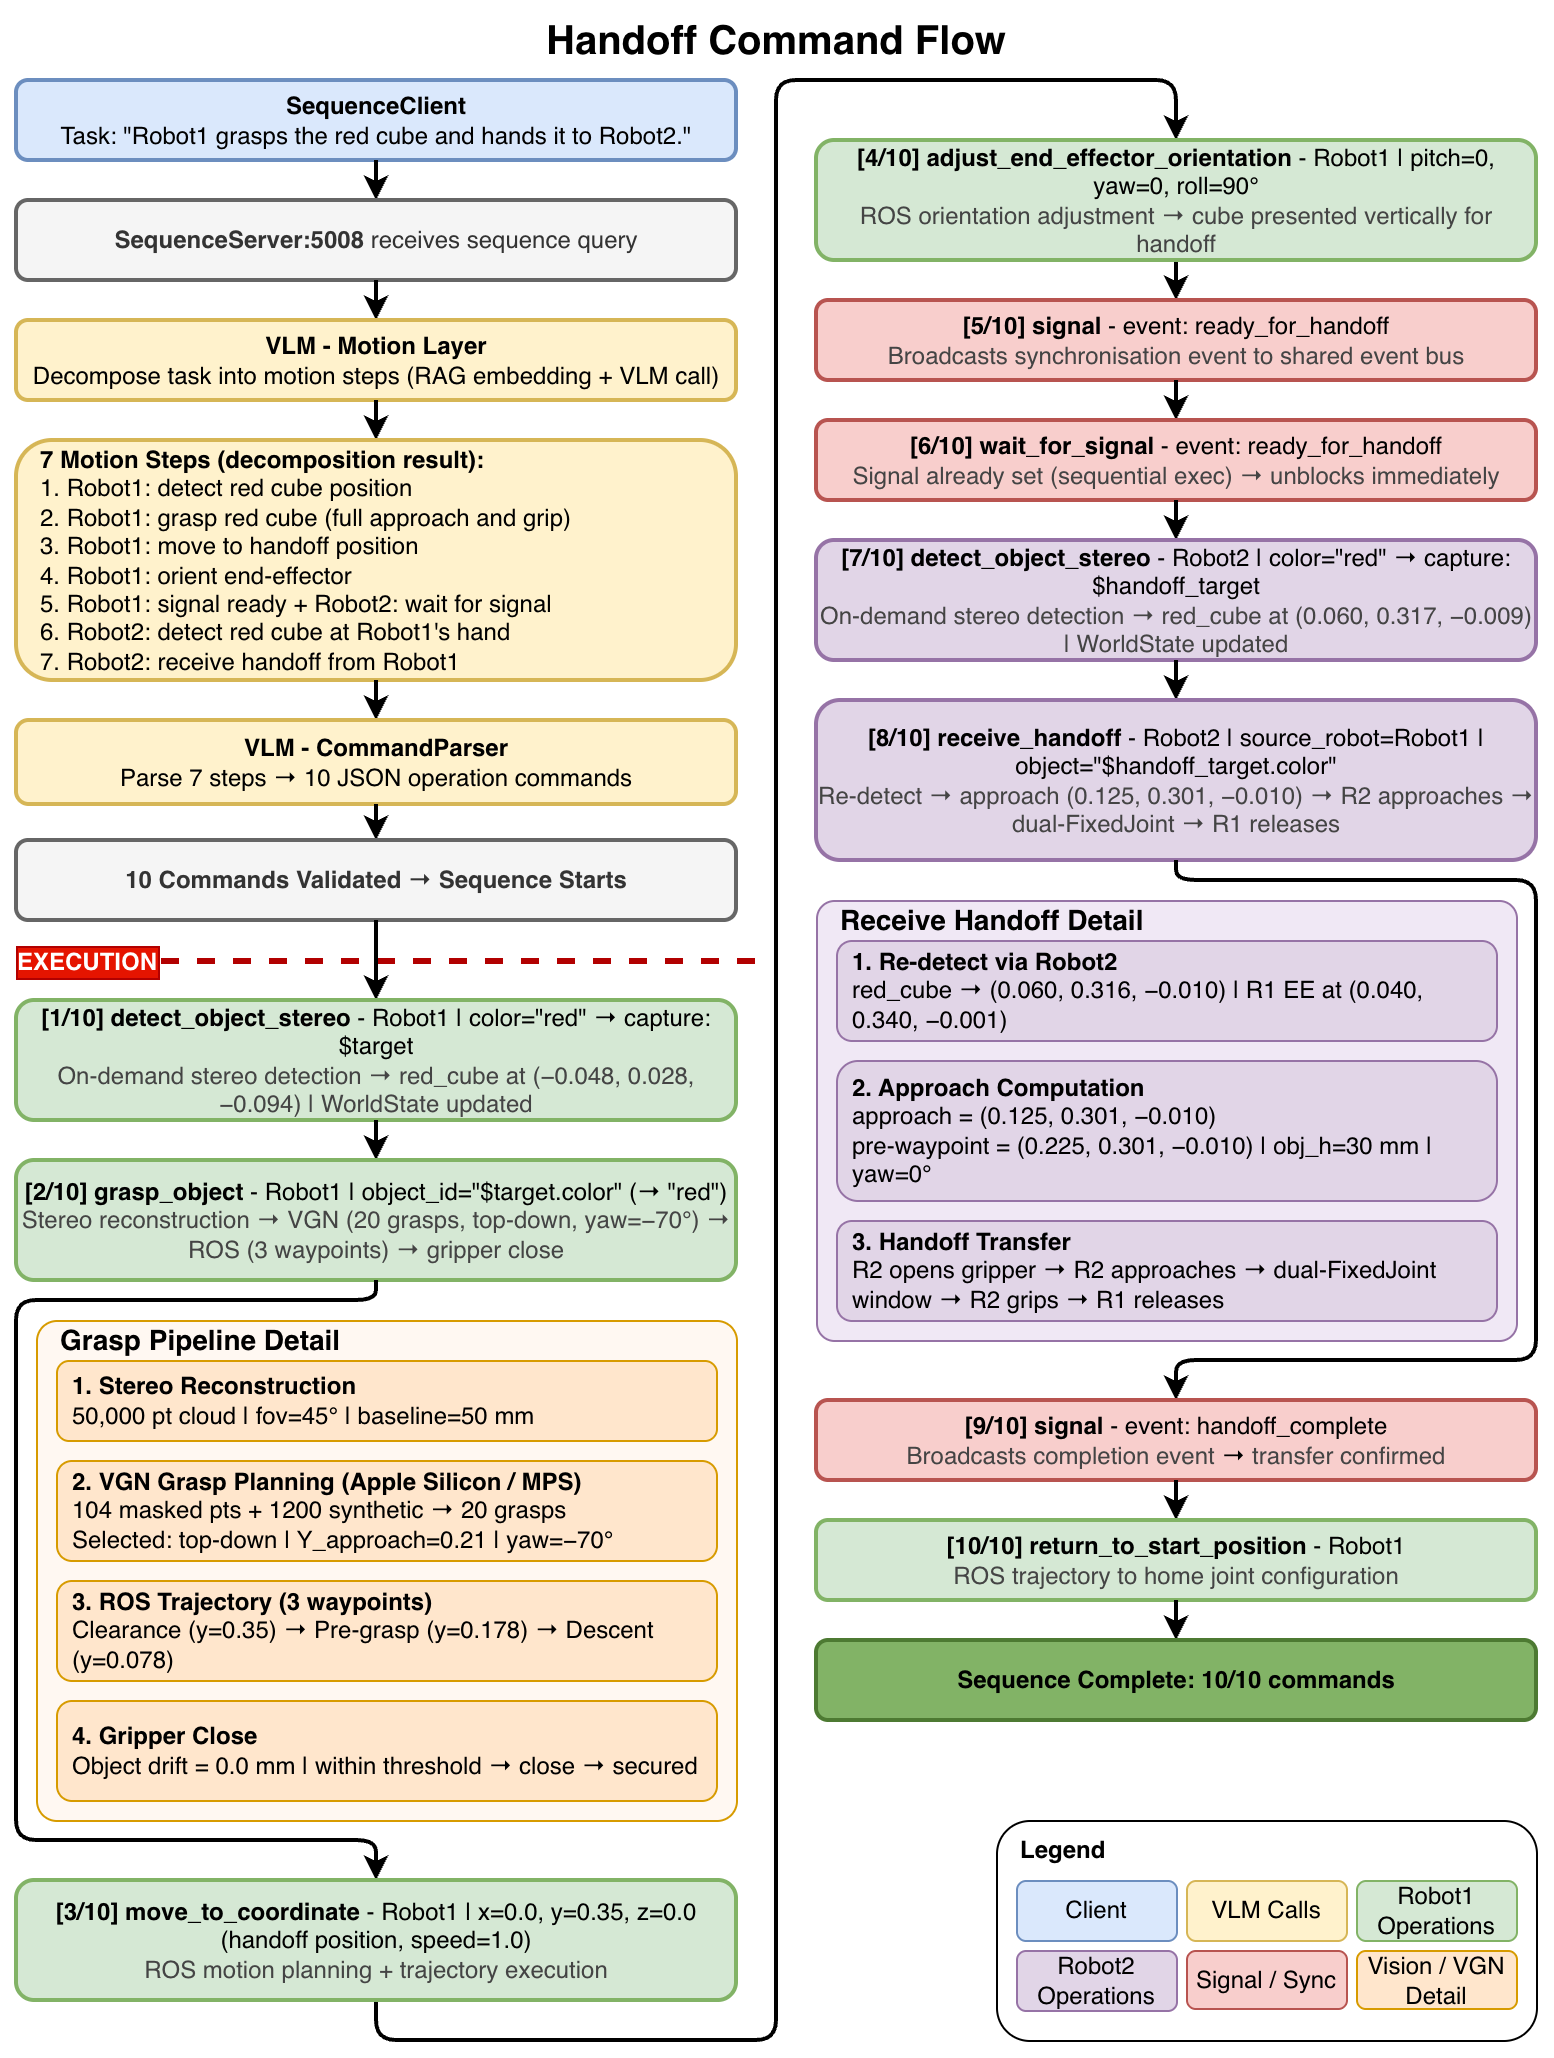
\includegraphics[width=1\linewidth]{images/12_handoff_sequence.png}
	\caption{A detailed flowgraph of how the handoff command is processed by the system.}
	\label{fig:handoff_flow}
\end{figure}

\begin{figure}
	\centering
	
\includegraphics[width=0.75\linewidth]{thesis/images/18_handoff_sequence_example.png}
	\caption{Accompanying motion of the two robots during the handoff sequence. Note the nine steps: the \texttt{grasp\_object} and \texttt{receive\_handoff} operations each expand into internal waypoint steps.}
	\label{fig:handoff_example}
\end{figure}

Figure~\ref{fig:handoff_flow} traces a complete handoff command through most of these layers, while Figure~\ref{fig:handoff_example} shows the resulting robot motion. The flowgraph serves as a structural reference while reading this chapter; the motion sequence illustrates the behavior the implementation produces. The full implementation is available on GitHub\footnote{\url{https://github.com/JanMStraub/Cooperative-Robot-Behavior-from-Basic-Action-Modules}}.

% ------------------------------------------------------------------------------
\section{System Infrastructure}\label{sec:infrastructure}
Before the system's intelligent components can do anything, several foundational pieces need to be in place: a physics-accurate simulation environment, a motion planning backend, and a communication layer that ties Unity and Python together. This section describes each of these in turn, focusing on the non-obvious engineering decisions and the problems that motivated them.

\subsection{Simulation Environment and Robot Control}\label{sec:sim-env}
The simulation runs in Unity 6000.3.11f1~\cite{unity} using the ArticulationBody physics component to model two AR4~\cite{AnninRobotics2026} 6-DOF robotic arms (Figure~\ref{fig:robot_env}). To obtain an accurate representation of the physical robot, we imported the actual \gls{urdf} files directly into the scene. ArticulationBody provides reduced-coordinate dynamics, so joint behavior stays physically plausible without the numerical drift that affects traditional Rigidbody chains. Each arm is driven by a three-layer control stack.

\begin{figure}
	\centering
	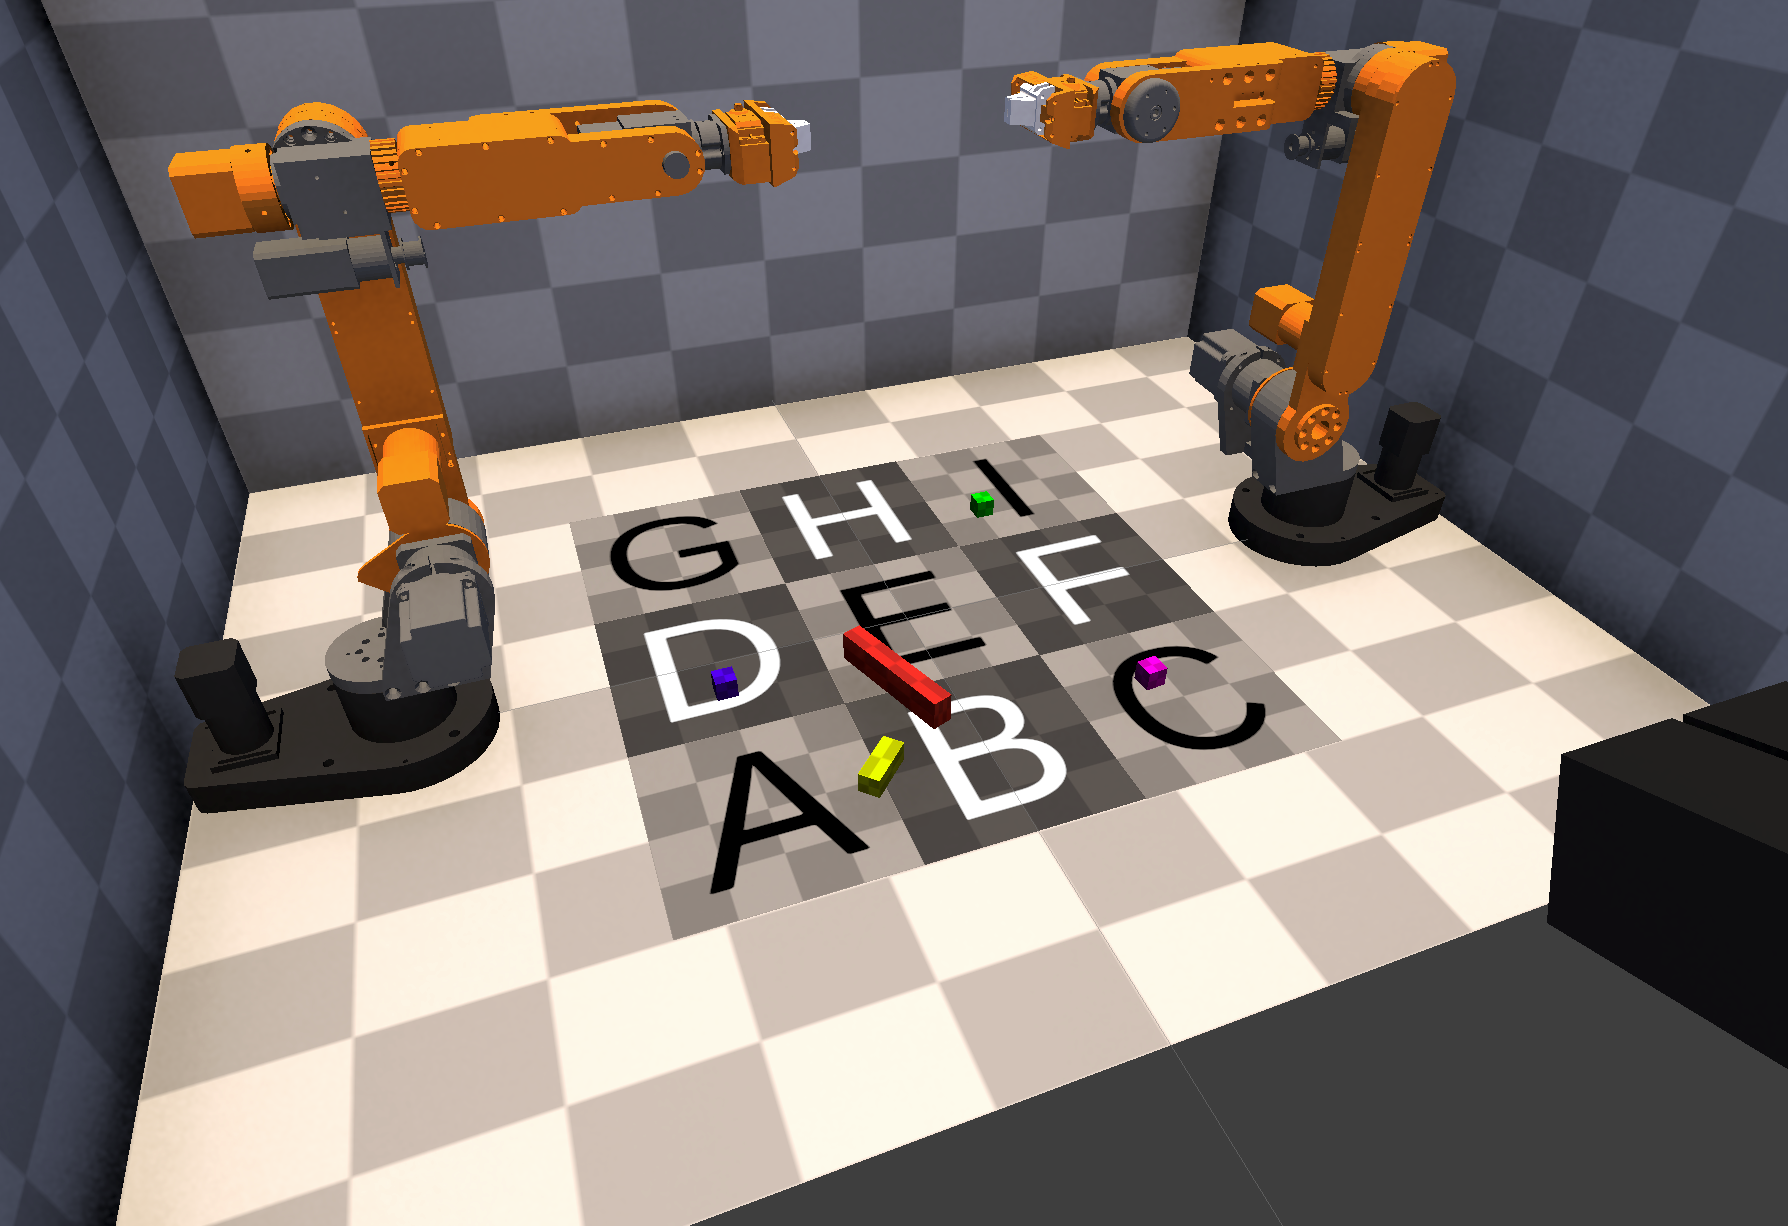
\includegraphics[width=0.5\linewidth]{images/14_robot_env.png}
	\caption{The Unity simulation environment showing the two AR4 robotic arms and the mutual workspace. Lettered zones are used for placing tasks, colored objects serve as manipulation targets, and the two black boxes on the right represent the stereo camera.}
	\label{fig:robot_env}
\end{figure}

At the bottom layer of this control stack lies the \gls{ik} solver, which uses damped least-squares to compute joint deltas from Cartesian error. An earlier version of the system oscillated, badly, from too large a per-frame step and too little damping. We added velocity feedback address this issue, so the joint update rule becomes

\begin{equation}
	\Delta\theta = J^{\dagger}_\lambda \bigl(K_p \cdot e_{\mathrm{pos}} + K_d \cdot e_{\mathrm{vel}}\bigr),
	\qquad
	J^{\dagger}_\lambda = J^{\top}\bigl(J J^{\top} + \lambda^2 I\bigr)^{-1}
\end{equation}

We use $K_p = 3.5$ and $K_d = 0.5$.\footnote{In the implementation, the combined error term $K_p \cdot e_{\mathrm{pos}} + K_d \cdot e_{\mathrm{vel}}$ is clamped to unit magnitude before the pseudo-inverse step. This guard, omitted from the idealized update rule above, prevents instability when a large target jump would otherwise produce an excessive single-step correction.} Joint velocities are clamped at 5.0 rad/s. The solver does not determine convergence. Instead, this is handled by the robot controller, which declares the target reached when the position error falls below an adaptive threshold (0.02 m by default, tightened for grasping) and the orientation error is within tolerance. The damping factor $\lambda$ is set to 0.2. The maximum joint step per iteration is capped at 0.2 rad.

The damped least-squares solver, however, is a local, gradient-based method. It minimizes Cartesian error by following the Jacobian gradient from the current joint configuration. Because it cannot avoid local minima or reason about the global joint-space landscape, two identical Cartesian targets can produce different joint configurations and approach paths depending on the initial state, rest pose, mid-task configuration, or a previous grasp. This results in two consequences. First, configurations near joint limits or wrist singularities can be unreachable from some starting poses, even when they are kinematically feasible from others, because the gradient path may hit a joint limit before reaching the target. Second, reproducibility can suffer, as runs starting from the home pose reliably converge, while those after a sequence can land in geometrically correct but mechanically awkward configurations, increasing settling time. To fix this, multi-phase benchmarks such as B8 issue an explicit \texttt{return\_to\_start\_position} command at the end of each phase, resetting the arm to a known well-conditioned configuration before the next task.

Above the \gls{ik} solver, a trajectory controller generates trapezoidal speed curves in Cartesian space, assuring controlled acceleration and deceleration instead of abrupt changes in target position. The trajectory controller operates with its own \gls{pd} gains, position gains of 10.0, and velocity gains of 2.0 per axis, governing how aggressively it tracks the desired profile. These are distinct from the \gls{ik}-level gains: the trajectory controller determines what the Cartesian target should be at any given instant, while the \gls{ik} solver translates each of those targets into joint-space commands.

We configure the ArticulationBody joints with per-joint stiffness and damping profiles tuned to each joint's mechanical characteristics. The base and shoulder joints, which bear the highest loads, use stiffness values of 4000--5000~N$\cdot$m/rad; the elbow joint uses 5000~N$\cdot$m/rad; and the wrist joints use 2500--3500~N$\cdot$m/rad. Damping was tuned empirically; the critical-damping condition $d = 2\sqrt{k \cdot I}$ serves only as a lower-bound reference, since at Unity's 50 Hz physics rate the joints require damping well above this baseline (see Appendix~\ref{appendix:robot_values}).

This three-layer control stack is only fully active in Unity mode. In the default Hybrid mode, each motion is attempted through MoveIt first and falls back to the Unity \gls{ik} and trajectory stack when planning fails, for instance, on a wrist singularity or an unreachable goal. In \gls{ros} mode, the \gls{ik} solver and trajectory controller are bypassed entirely, and MoveIt computes every joint trajectory, which Unity receives over the \gls{ros}-TCP bridge and executes directly through the ArticulationBody joints. The \gls{ros} implementation is described in detail in Section~\ref{sec:ros_moveit}.

\begin{figure}
	\centering
	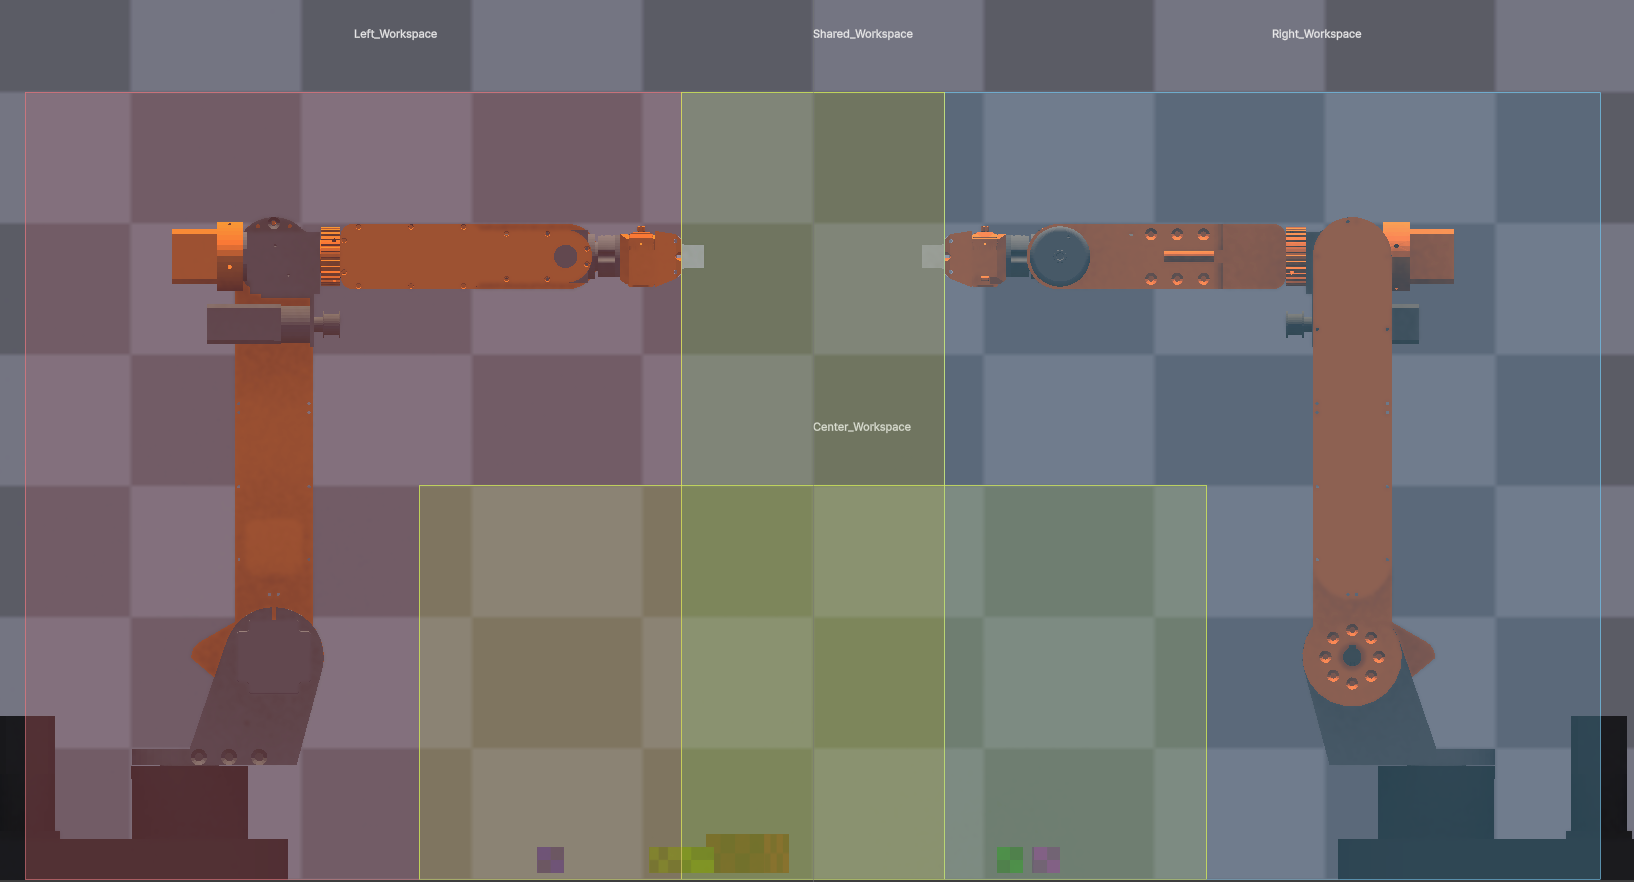
\includegraphics[width=0.75\linewidth]{images/15_robot_workspaces.png}
	\caption{Workspace regions defined in Unity, used by the knowledge graph and the evaluation benchmarks. Red and blue mark each robot's primary zone; the yellow areas are the center and shared zones where the two arms may interact.}
	\label{fig:robot_workspaces}
\end{figure}

Safety limitations operate in three distinct layers. At the Python level, \texttt{CoordinationVerifier} runs a static pre-check before every navigation command, and if the planned target falls within 60~mm of the partner robot's current end-effector position, the command is blocked, and a safe waypoint is prepended to the resolution suggestions before dispatch. When both robots are moving, a separate, looser check compares the two planned targets against a 0.2~m minimum separation; this is the check the concurrent lift in B7 violates (Section~\ref{sec:results-dual}). The same pass also checks for workspace conflicts, object conflicts (both robots targeting the same grasped object), and potential deadlocks.

At the Unity level, the \texttt{ProximityGuard} monitors end-effector separation at runtime. When the separation drops below 0.25~m, both robots are frozen and unfreeze automatically once the separation clears 0.35~m. Link-to-link proximity for joints 2--5 is checked separately with a tighter 0.15~m threshold, since mid-arm collisions can happen even when end-effectors are far apart. The frozen state is broadcast to Python on the next \texttt{WorldStatePublisher} cycle, allowing the planner to replan rather than wait indefinitely. During intentional close-approach operations such as handoffs, the \texttt{ProximityGuard} is disabled by the \texttt{receive\_handoff} operation and re-enabled on completion, because those sequences handle inter-robot safety internally through the signal/wait serialization protocol.

The third safety layer is the workspace region system (Figure~\ref{fig:robot_workspaces}). The workspace is divided into four named regions: \texttt{left\_workspace} ($-0.6 \leq x \leq -0.1$~m, Robot~1's main area), \texttt{right\_workspace} ($0.1 \leq x \leq 0.6$~m, Robot~2's main area), \texttt{shared\_zone} ($-0.1 \leq x \leq 0.1$~m, the overlap of both robots' allocations), and \texttt{center} (overlaps with the shared zone and inner parts of both workspaces, used by the knowledge graph for proximity reasoning). Region ownership is tracked by Python's \texttt{WorldState}. Enforcement occurs through the \texttt{yield\_workspace} operation, which causes a robot to release its current region so the partner may enter. This strict region partition differs from the per-robot reachability bounds provided to the command-parser model in its prompt (Appendix~\ref{appendix:prompts}), which extend each arm to $|x| \leq 0.165$~m and therefore overlap the shared zone. The looser reachability bounds reflect the kinematic reach across the centerline, whereas the tighter $\pm0.1$~m \texttt{shared\_zone} sets the explicit boundary for region allocation and coordination.

\subsection{Grasp Planning Pipeline}
Grasping is handled by a four-stage pipeline inspired by the MoveIt grasp planning architecture, implemented separately on both the Unity and Python sides. The two implementations share the same logical structure: candidate generation, \gls{ik} filtering, collision filtering, and scoring, but serve different execution paths. The Unity pipeline plans grasps for the built-in \gls{ik} stack, while the Python pipeline (\texttt{grasp\_planning/}) plans for the \gls{ros}/MoveIt path and validates its candidates directly against MoveIt's \gls{ik} solver. Table~\ref{tab:grasp_params} lists the key parameter differences.

\begin{table}[ht]
	\centering
	\begin{tabular}{lcc}
		\hline
		\textbf{Parameter}             & \textbf{Unity} & \textbf{Python} \\
		\hline
		Candidates per direction       & 10             & 8               \\
		Angle perturbation             & $\pm20^\circ$  & $\pm15^\circ$   \\
		Maximum reach                  & 0.6 m          & 0.75 m          \\
		\gls{ik} validation iterations & 250            & 50              \\
		\gls{ik} validation threshold  & 0.01 m         & 0.005 m         \\
		Depth score weight             & 0.6            & 1.0             \\
		Pipeline time budget           & 1000 ms        & 200 ms          \\
		\hline
	\end{tabular}
	\caption{Grasp planning parameters for the Unity (\texttt{GraspConfig.asset}) and Python (\texttt{grasp\_planning/GraspConfig.py}) implementations. We tuned the Unity values for execution under PhysX: a generous \gls{ik} budget and a tighter 0.6~m reach keep candidates where the damped least-squares solver converges reliably, while the Python pipeline can afford a tighter validation threshold and shorter time budget because its candidates are checked against MoveIt's \gls{ik} solver.}
	\label{tab:grasp_params}
\end{table}

The candidate generator produces proposals for three approach directions: top, front, and side with approach-angle perturbations and object-size-adaptive pre-grasp distances ranging from 5 to 15 cm. Candidates pass through an \gls{ik} filter that first applies a fast distance-based reachability check and then a full \gls{ik} validation. Those that survive are evaluated by a collision filter, which samples five waypoints along the approach trajectory and performs sphere-cast checks within a 3 cm radius at each waypoint. The final scorer combines five weighted additive criteria: \gls{ik} quality (weight 1.0), approach direction preference (0.8), grasp depth relative to the object center (0.6 Unity / 1.0 Python), stability based on contact geometry (1.2), and antipodal quality (1.0), all scaled by an orientation-consistency multiplier. We gave the stability term the highest weight because empirical tuning showed it was the strongest predictor of whether the grasp would withstand the forces encountered during subsequent manipulation.

Grasp verification after closing is handled by a contact sensor that tracks per-finger contact via Unity's collision callbacks, applies a 5-frame moving average to smooth physics noise, and requires a minimum contact duration of 50 ms and an estimated contact force above 5 N before declaring a successful grasp.

When a higher-quality grasp pose is needed, particularly for handoff tasks where the receiving robot requires a predictable object orientation, the \gls{vgn} pipeline~\cite{breyer2021volumetricgraspingnetworkrealtime} is a viable alternative. It takes a \gls{yolo} bounding box, constructs a masked point cloud, builds a \gls{tsdf} volume, and runs \gls{vgn} inference to produce 6-DOF grasp poses. These candidates are injected into the same filter and scorer pipeline, with a fallback to the heuristic planner if all \gls{vgn} candidates are rejected.

We first tried Contact-GraspNet~\cite{sundermeyer2021contactgraspnetefficient6dofgrasp} as the data-driven backend. However, it requires a dedicated GPU for inference, which we did not have in our development environment, so we adopted \gls{vgn} instead. Its lighter inference footprint runs on the CPU and Apple Silicon without modification, which fits the infrastructure-independent deployment goals from Section~\ref{sec:local}. While \gls{vgn} is trained on both top-down and side grasps, the sparse \gls{tsdf} volumes produced by this system's stereo disparity cause it to favor top-down candidates in practice. This limits its effectiveness for objects that require a lateral approach. Section~\ref{sec:perception-depth} analyzes the underlying stereo depth limitation, and the effects on the combined \gls{vgn}/\gls{ros} execution path are examined in Section~\ref{sec:results-vgn}.

\subsection{ROS and MoveIt Integration}\label{sec:ros_moveit}
MoveIt is integrated as an optional planning backend rather than a full robot controller. Our key implementation choice is to enable the \texttt{plan\_only} flag in the MoveGroup goal: MoveIt produces a joint trajectory plan but does not attempt to execute it. Unity receives the trajectory over the \gls{ros}-TCP bridge and executes it through its ArticulationBody physics, avoiding the requirement for a \gls{ros} control hardware interface.

The three control modes introduced in Section~\ref{sec:sim-env} vary mainly in planning cost and collision handling. \gls{ros} mode plans through MoveIt, typically completing in under 0.5~s with execution taking 2--10~s, and provides full collision-aware planning via \gls{ompl}~\cite{6377468}. Unity mode is preferable when lower latency matters and collision-aware planning is not required; \gls{ros} mode becomes worthwhile once the workspace is cluttered enough to need collision-free planning. Hybrid, the default, takes the collision-aware MoveIt path when planning succeeds and the low-latency Unity path when it does not.

Joint states are published at 50~Hz using pre-allocated \gls{ros} messages to avoid garbage-collection pressure. Trajectories are received and validated against joint limits and velocity constraints, and interpolated to Unity's fixed-update frequency. In dual-robot mode, all topics are namespaced per robot to keep the two control streams independent.

We encountered three failure modes during integration, each calling for an explicit fix before the \gls{ros}/MoveIt path became reliable.

\paragraph{MoveIt \texttt{UNKNOWN\_ERROR\_99999}.}
\gls{ompl} aborted planning with error code 99999 in two distinct scenarios. First, Unity's ArticulationBody physics can overshoot joint limits at the end of a trajectory, particularly after a settle timeout. Submitting those out-of-bounds values as the MoveIt start state causes \gls{ompl} to reject it as kinematically invalid; our fix clamps every joint value to its \gls{urdf} bounds before constructing the \texttt{RobotState} message. Second, setting \texttt{is\_diff = false} at the start state caused unlisted joints to default to zero, placing the robot in self-collision or in contact with the ground plane, and triggering the same error. Setting \texttt{is\_diff = true} instructs MoveIt to apply the provided joints as a differential update over its internally tracked state, leaving unlisted joints unchanged. Additionally, gripper jaw joints published by Unity must be stripped from the start state prior to submission, as the \texttt{arm} planning group does not include them, and their presence renders the start state invalid.

\paragraph{Execution settle timeout.}
Unity sends a \texttt{completed\_with\_timeout} status when trajectory execution finishes, but the arm has not fully settled at its drive target within the allotted window. If the next plan is requested immediately, MoveIt receives a stale \texttt{/joint\_states} that still reflects the arm mid-motion, producing a start state that either violates joint bounds or sits in an unexpected configuration. Our fix inserts a 3~s physics-settle wait after any \texttt{completed\_with\_timeout} response before the next planning request is issued. The execution timeout itself is set dynamically as
\begin{equation}
	t_{\mathrm{exec}} = \max\!\bigl(c_0,\; 2.5 \cdot t_{\mathrm{traj}} + c_1\bigr)~\text{s},
\end{equation}
where the floor $c_0$ and offset $c_1$ are set per call path (for example $c_0 = 30$, $c_1 = 15$ on the primary plan-and-execute path), so the timeout scales conservatively with trajectory duration.

\paragraph{\gls{vgn} approach bias.}
When stereo point cloud quality is insufficient to produce reliable \gls{tsdf} input, \gls{vgn} generally prioritizes candidates whose approach vectors are biased toward the vertical. Selecting the highest-scoring candidate without filtering in these cases yields a near-vertical approach direction, causing the wrist to rotate into a twisted configuration unsuitable for lateral grasps. Our resolution is a threshold on the approach vector's vertical component: if the \gls{vgn} approach $Y$ component is at least $0.7$, we trust the vector and use it directly. Otherwise, in the common case where \gls{vgn} returns a not-quite-vertical vector, the approach vector is overridden with a proven straight-up top-down direction.

\subsection{Communication Architecture}\label{sec:communication}
The Unity simulation and the Python backend communicate over TCP. Table~\ref{tab:ports} lists the active server ports.

\begin{table}[ht]
	\centering
	\resizebox{\textwidth}{!}{%
		\begin{tabular}{rllp{6cm}}
			\hline
			\textbf{Port} & \textbf{Server}        & \textbf{Direction}               & \textbf{Purpose}           \\
			\hline
			5006          & ImageServer            & Unity $\to$ Python               & Stereo image pairs         \\
			5007          & CommandServer          & Bidirectional                    & Commands and results       \\
			5008          & SequenceServer         & Bidirectional                    & Multi-command sequences    \\
			5009          & WorldStateServer       & Unity $\to$ Python               & Robot and object state     \\
			5010          & AutoRTServer           & Bidirectional                    & Autonomous task generation \\
			5020          & \gls{ros}Bridge        & Python $\leftrightarrow$ Docker  & MoveIt motion planning     \\
			8000          & WebUIServer            & Browser $\leftrightarrow$ Python & Mission Control dashboard  \\
			10000         & \gls{ros}-TCP-Endpoint & Unity $\leftrightarrow$ Docker   & \gls{ros} topic bridge     \\
			\hline
		\end{tabular}
	}
	\caption{Active TCP server ports and their roles.}
	\label{tab:ports}
\end{table}

All messages use a protocol, which prepends a 5-byte header to each message: one byte for the message type and four bytes for the request identifier. The request ID enables asynchronous request-response matching, as the Python backend maintains per-request queues and handles concurrent operations from multiple robots without mixing replies.

World state is published on a dedicated port as a one-way broadcast stream with a fixed request ID of zero, explicitly separating it from the request--response channel. We introduced this separation after early versions suffered correlation errors when high-frequency world-state updates arrived interleaved with command responses.

End-to-end, a command flows as follows: a natural-language sequence arrives at the Python \texttt{SequenceServer}; the backend passes it to the command parser; the parsed plan goes to the sequence executor, which dispatches each operation through the ROS-vs-Unity router. In the default Hybrid mode, motion commands are planned by MoveIt and the resulting trajectory is executed by Unity through its ArticulationBody physics, falling back to the Unity \gls{ik} pipeline when planning fails; Unity then returns a completion notification. In practice, model parsing is the dominant fixed cost: the median time from query arrival to validated plan was roughly 18~s, driven by the reasoning model's thinking budget. Motion planning adds well under 0.5~s on the \gls{ros} path (or 5--10~ms per \gls{ik} step on the Unity path), and robot movement 2--10~s per motion command depending on travel distance, so a complete command sequence typically finishes within 30--60~s of arriving.

On top of this TCP backbone is an optional operator interface, the Mission Control dashboard, served by a FastAPI gateway (\texttt{WebUIServer}) on port 8000 and enabled with the \texttt{--web} flag. Unlike the Unity-facing servers in Table~\ref{tab:ports}, it acts purely as a client of the existing backend: it subscribes to the world-state broadcast and command results to render the live scene, streams backend logs and AutoRT task proposals, lets an operator issue natural-language commands, and exposes the benchmark analysis tab used throughout Chapter~\ref{evaluation}. The dashboard is fully decoupled from the system; it runs headless, serving as a diagnostic and control surface rather than a part of the control loop.

% ------------------------------------------------------------------------------
\section{Operations System}\label{sec:ops-impl}
Each operation is an instance of the \texttt{BasicOperation} dataclass, configured with an implementation callable; its shared \texttt{execute()} method validates parameters and dispatches to that callable, returning an \texttt{OperationResult} containing a success flag, an optional error dictionary, and a result dictionary. Operations are registered in a central registry at startup, which serves as the single source of truth for the \gls{rag} indexer, the command parser prompt, and the AutoRT task generator.

Beyond the operation implementations themselves, each operation carries structured metadata that the \gls{rag} system actively uses. \texttt{ParameterFlow} objects declare how output fields of one operation map onto input parameters of another, allowing the retrieval step to surface both the most relevant individual operation and the natural sequences it belongs to. Eight such flows are defined across the registry, covering vision, field, and spatial operations. \texttt{OperationRelationship} objects declare which operations are commonly paired together and what temporal ordering constraints exist between them.

An example of an operation can be found in Appendix~\ref{appendix:operation_example}.

% ------------------------------------------------------------------------------
\section{Intelligent Task Planning}\label{sec:planning-impl}
This section covers the concrete implementation of the command pipeline described in Section~\ref{sec:command-pipeline}: how we serve and configure the local model, build and query the \gls{rag} index, and convert a retrieved plan into robot actions.

\subsection{Local Model Selection}
The locally hosted \gls{vlm} is served via LM Studio~\cite{lmstudio}, which exposes an OpenAI-compatible API endpoint. We chose this interface because it lets the same client code target different models without modification, making model substitution straightforward during evaluation. Temperature is set to 0.3 for command parsing, low enough to keep plan generation predictable. To improve output quality on multi-step tasks, we use two complementary mechanisms: a model-level thinking block, enabled via LM Studio's \texttt{budget\_tokens} parameter, that lets the model reason internally before producing a response; and a chain-of-thought context injected into the prompt as motion-planning guidance. Together, these reduce structural errors in the generated plans, though we have not independently measured the effect of each mechanism.

\subsection{RAG System and Embedding}
Embeddings are generated using \texttt{nomic-embed-text-v1.5}~\cite{nussbaum2025nomicembedtrainingreproducible}, served locally via LM Studio and producing 768-dimensional vectors. If LM Studio is unavailable at startup, the system falls back to TF-IDF with a maximum of 500 features, which is coarser, but sufficient to keep the system functional in degraded conditions. The vector store uses cosine similarity search with an in-memory index protected by a thread-safe lock; the index is persisted to disk, so re-indexing is needed only when operations change. Query results are filtered by a minimum similarity threshold of 0.5 and a configurable confidence strategy (strict / balanced / permissive). Figure~\ref{fig:rag} shows the indexing and search pipeline.

\begin{figure}
	\centering
	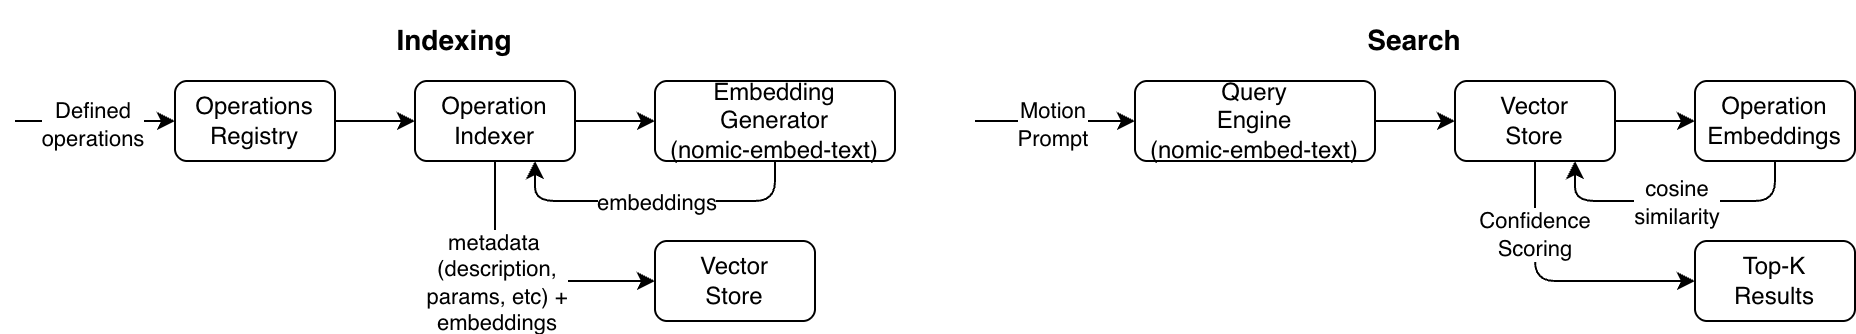
\includegraphics[width=1\linewidth]{images/13_rag.png}
	\caption{Indexing and search in the \gls{rag} system: operations are embedded and stored at startup (left); a user prompt is embedded and matched by cosine similarity, then confidence-scored to Top-K results (right).}
	\label{fig:rag}
\end{figure}

The \gls{rag} index contains 42 items in total: the 29 registered operations, 9 predefined workflow patterns, and 4 multi-robot context documents. The workflow patterns describe common multi-step sequences in a structured form, including pattern-level success criteria and recovery hints for failures. When one scores highly during retrieval, it is injected into the model prompt as an example plan, which reduces structural errors in generated plans for familiar task types. The context documents cover workspace layout, coordination patterns, safety restrictions, and parallel execution guidelines, giving the model relevant background when no single operation is a close semantic match to the query.

\subsection{Command Parser and Sequence Executor}
The command parser extracts and normalizes the JSON from the model's response. A 90-second timeout is applied per request, and a connection pool with 10 persistent connections reduces TCP overhead. The system prompt lists the top \gls{rag}-retrieved operations with their full parameter schemas: the vector store is queried for 10 candidates, of which up to 5 operations and up to 3 workflow patterns are retained, along with critical rules for multi-robot tasks and the variable-passing syntax.

Before execution, the parser validates the returned plan: operation names are checked against the registry, and every \texttt{wait\_for\_signal} call must have a matching \texttt{signal} with the same identifier. Variable references are resolved at execution time; unresolved references fall back to recovery patterns or are left for the operation's parameter type-check to reject, and missing \texttt{capture\_var} declarations are inferred from downstream \$var usage. If the response can be partially salvaged, for example, if the model returned a bare array instead of a wrapped object, a normalization step is attempted before returning an error. If LM Studio~\cite{lmstudio} is entirely unreachable, the parser falls back to a regex-based matcher that covers a subset of common command patterns.

The sequence executor iterates over the validated plan. For operations sharing the same parallel group identifier, it dispatches them concurrently and blocks until all complete or a timeout elapses. The group timeout is derived from the per-command timeout plus a 5-second overhead, giving 125 seconds under the default configuration. Variable passing is handled automatically: after each operation, result fields declared in the operation's parameter flow metadata are stored in a session-scoped variable dictionary; before each operation, missing parameters are filled from this dictionary by field-name matching. Both explicit capture directives in the plan and automatic capture run in sequence, with explicit directives applied first. Signal and wait primitives are implemented using a \texttt{threading.Condition} variable: the signaling robot calls \texttt{notify\_all()} on the condition, and the waiting robot blocks on the condition until notified, a true blocking wait rather than a polling loop.

\subsection{Reflection Strategy}
When an operation fails, the executor checks whether it qualifies for reflection-based recovery. Only Navigation, Manipulation, and Perception category operations are eligible; synchronization primitives and status checks are explicitly excluded, since re-querying the language model for them offers no benefit and adds latency. If the failed operation is eligible and reflection is enabled, the executor constructs a failure hint by combining the error message with any recovery suggestions returned by the failed operation. This hint is returned to the command parser alongside the original natural-language command, which re-queries \gls{vlm} with the failure context appended. The re-parsed command is re-resolved against the current variable store and re-executed. This loop runs up to 2 retries by default; on success, the failed entry in the sequence log is replaced with the successful result, and execution continues normally.

\subsection{Knowledge Graph}
The \gls{kg} is implemented as a thread-safe directed multi-graph using NetworkX, wrapped by a reentrant lock to permit concurrent reads from the world-state callback thread and from operation handlers. A secondary type index enables constant-time lookup by entity class, avoiding full-graph scans for common queries. The graph is rebuilt on every world-state update by a builder that registers as a callback on the world-state server. Three node types represent robots, objects, and workspace regions. Six edge relations are actively populated: \textsc{Can\_Reach}, \textsc{Near}, \textsc{In\_Region}, \textsc{Grasping}, \textsc{Adjacent\_To}, and \textsc{Allocated}. The graph can be serialized to GraphML for offline analysis. Figure~\ref{fig:kg_example} shows the graph state at simulation start.

\begin{figure}
	\centering
	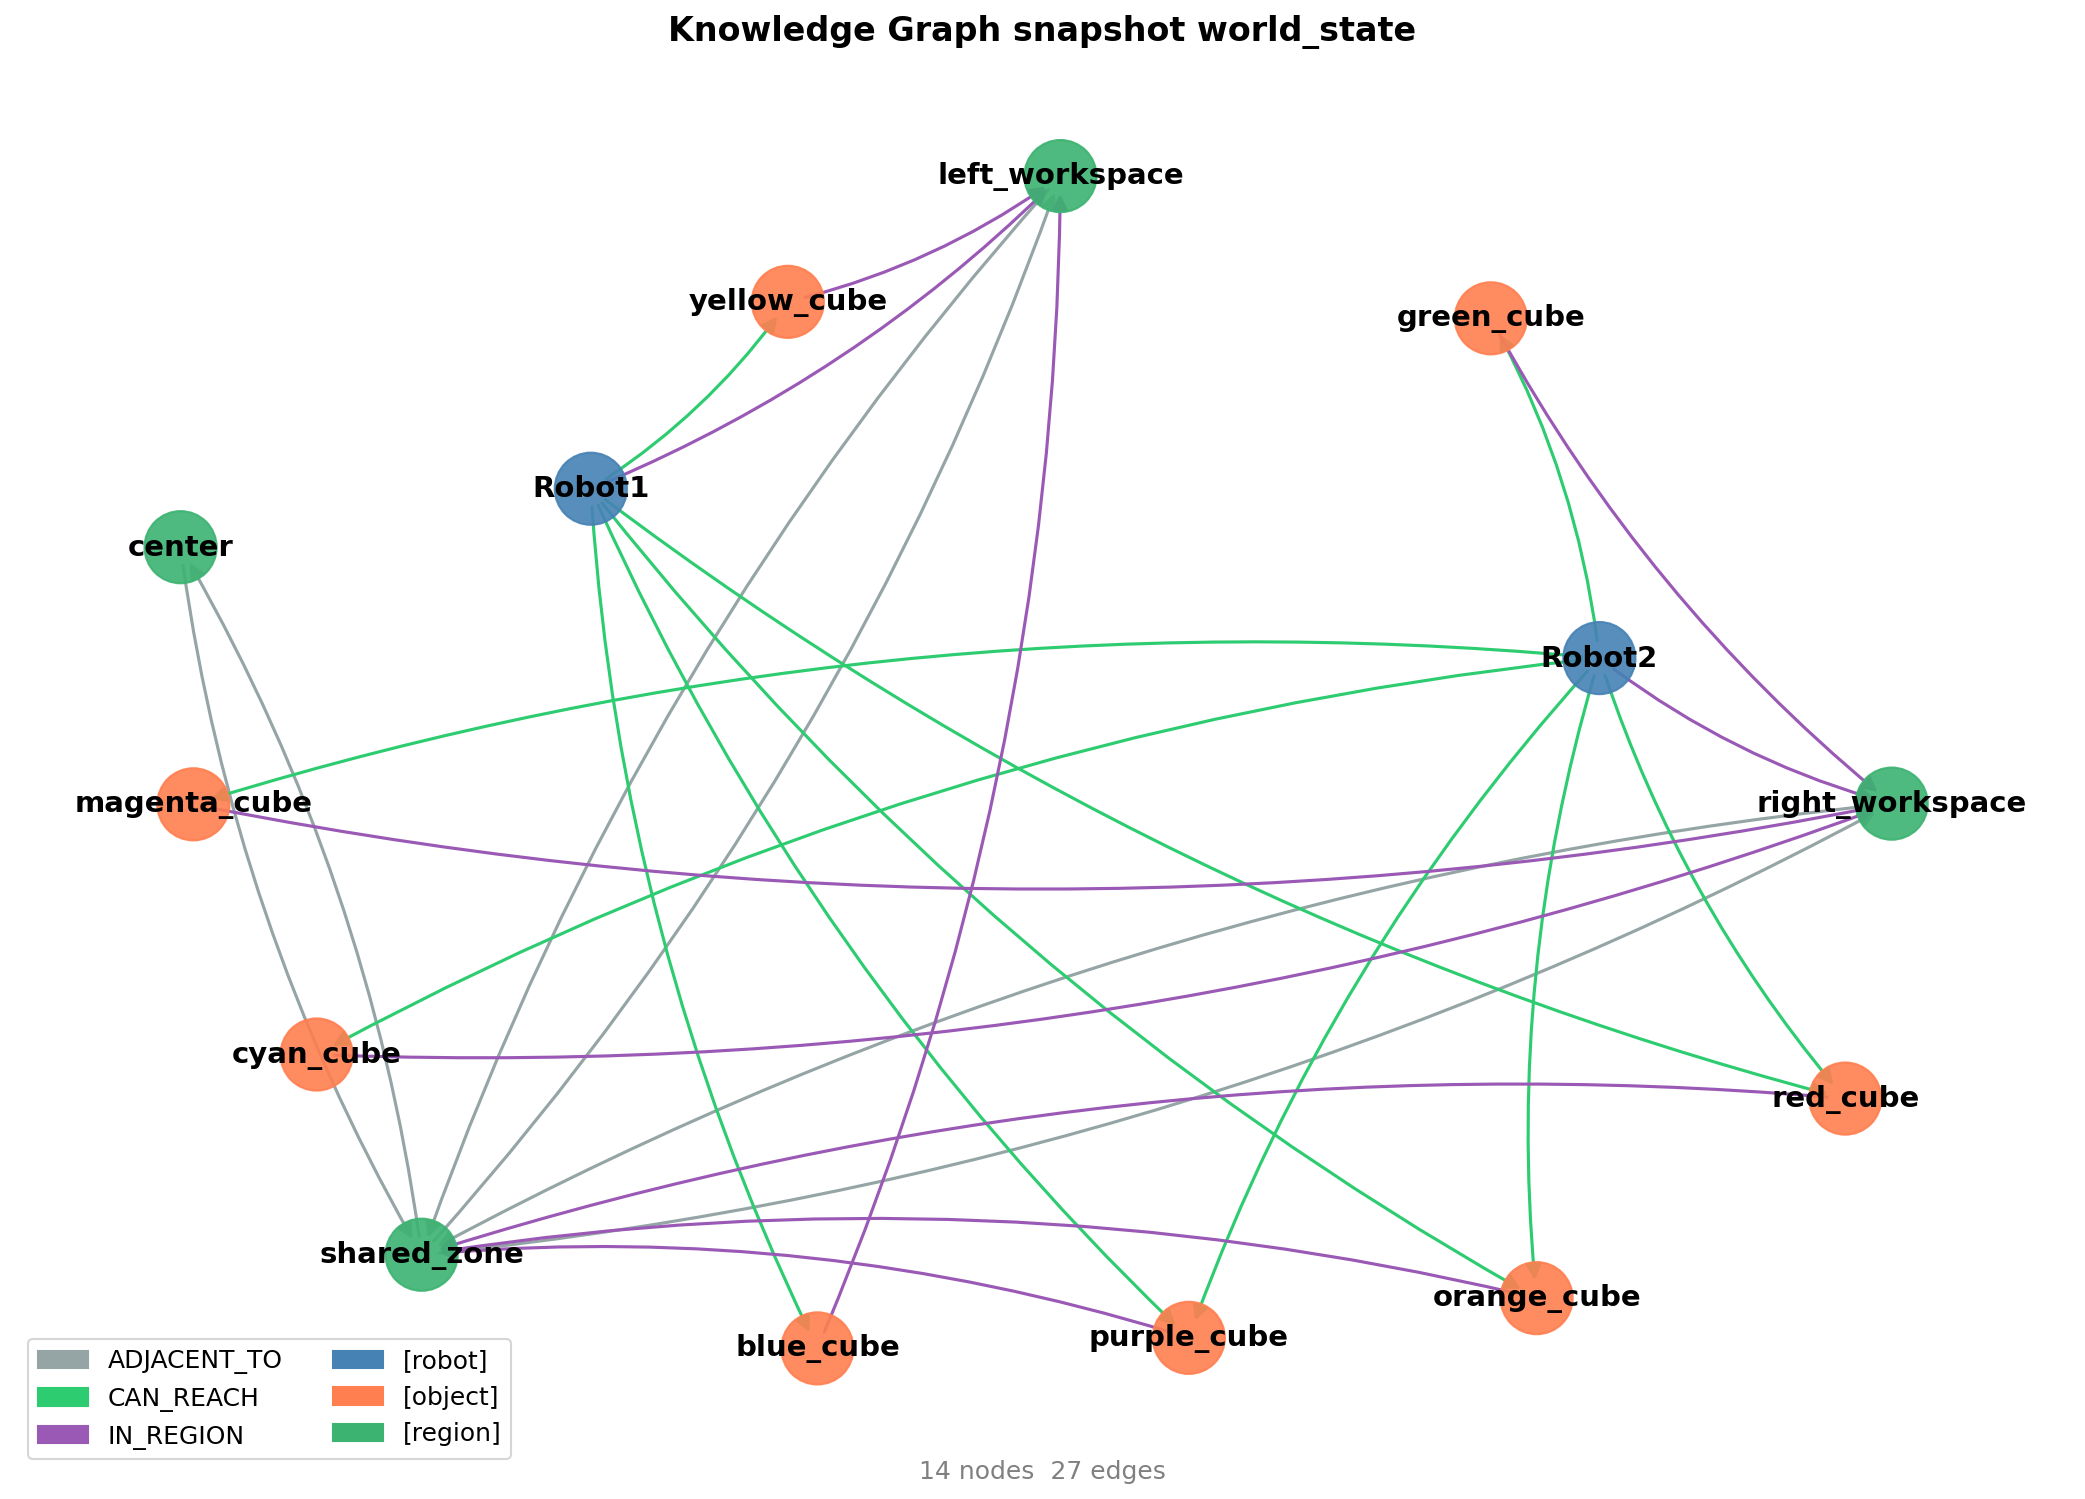
\includegraphics[width=0.75\linewidth]{images/11_kg_world_state.png}
	\caption{The \gls{kg} at simulation start: robot, object, and region nodes with their initial reachability, proximity, and containment edges.}
	\label{fig:kg_example}
\end{figure}

% ------------------------------------------------------------------------------
\section{Benchmark Implementation}\label{sec:benchmark-impl}
Each benchmark is implemented as a self-contained Python module. The single-task benchmarks (B1--B7, B9, B10) expose a \texttt{get\_task()} function that returns one natural-language task; the ablations (B11--B16) expose \texttt{get\_tasks()} returning a list, and B8 exposes \texttt{get\_sub\_tasks()}. The \texttt{BenchmarkRunner} dispatches this string to the live system over the same TCP interface used in normal operation, connecting to the \texttt{SequenceServer}. Most execution benchmarks send the task string through the full parsing pipeline. Two exceptions, B15 (\gls{vgn}) and B16 (\gls{ros}-vs-Unity), dispatch fixed operation chains directly to the sequence executor and bypass the command parser so that grasp quality and movement timing are measured independently of parser variability. For the rest, the command parser translates the natural-language instruction into an ordered list of operations, which the sequence executor then executes in the simulation. This tests the correctness of the full pipeline rather than just low-level execution.

Three benchmarks stop earlier in the pipeline: B9 runs in parse-only mode to evaluate input rejection, and the B11 and B14 ablations evaluate parse quality without dispatching operations to Unity. B17 is the most self-contained of all: it bypasses the \texttt{BenchmarkRunner} dispatch entirely and drives \texttt{RobotConstitution.evaluate\_task()} and the task generator in process, so it runs fully offline with only the local model and no Unity or server stack (Section~\ref{sec:results-autort}).

Results are collected as a \texttt{BenchmarkResult} dataclass capturing step-level metrics, operation name, duration, success flag, and error information alongside aggregate figures: total wall-clock duration, operations executed and succeeded, per-benchmark success rate, mean step duration, and the index of the first failing step. Each run is tagged with a unique identifier that combines a UTC timestamp and a UUID fragment, enabling each run to be uniquely identified and traced. A run is marked successful if and only if the sequence executor reports success for the entire sequence, inheriting the operation-level pass/fail semantics already defined in the system. Benchmark B8 departs from the single-sequence model. Instead of a single fixed task, the runner issues a scripted sequence of 20 heterogeneous natural-language prompts, organized into four phases, repeated over five cycles each, parsed and executed as independent sequences without cross-prompt memory. The chain succeeds only if every sub-task succeeds and every parsed plan fits the expected operation template, making B8 a measure of sustained system reliability rather than single-task capability.

Between every run, a reset command returns all objects and robots to their initial poses to ensure isolation between trials. A dry-run mode bypasses TCP entirely and executes operations in-process, enabling fast testing of benchmark logic without a running simulation.

% ------------------------------------------------------------------------------
\section{Autonomous Task Generation and Coordination}\label{sec:autort-impl}
This section covers the implementation of the system's autonomous capabilities, how it perceives the scene, generates and filters task candidates, and coordinates activities across two robots. It corresponds to the methods described in Sections~\ref{sec:negotiation} and~\ref{sec:autort}.

\subsection{Vision System}
Object detection uses a fine-tuned \gls{yolo}v8~\cite{yolov8_ultralytics} model trained on a custom cube dataset, with 17 object classes covering manipulation targets and workspace field markers. The model is loaded at runtime from an \gls{onnx} file, with the actual class count determined by the model metadata. Images are captured from Unity simulation cameras. Depth estimation uses a stereo camera pair with a 5 cm baseline and 45$^\circ$ field of view. Stereo disparity is computed using OpenCV's \gls{sgbm}~\cite{4359315} algorithm with a tuned preset. We found the defaults unnecessarily expensive for the object distances in our workspace; switching to asynchronous image transfer and batching \gls{yolo} inference dropped detection latency.

Persistent object tracking between frames uses intersection-over-union matching. Each track maintains a position history used for velocity-based prediction, and it is aged out after 5 consecutive frames without a match. In multi-robot scenarios, a common vision state module provides a thread-safe object registry with a claim/release mechanism: when one robot claims an object, the other robots see it as unavailable. Stale claims are released after a 10-second timeout, with conflict resolution defaulting to closest-robot priority.

We designed the vision system as an interchangeable component via an abstraction of camera providers. In simulation, a Unity adapter wraps the Unity image store; in real-robot mode, a local adapter connects to cameras instead. No other system component needs to distinguish between the two.

\subsection{AutoRT Implementation}
The AutoRT~\cite{ahn2024autortembodiedfoundationmodels} loop runs only when it is triggered manually. Each iteration begins with scene capture: stereo object detection retrieves a complete list of grounded objects with 3D positions, the world state provides robot positions and gripper states, and an optional \gls{vlm} call adds a semantic scene summary. Duplicate objects between stereo detection and the world state are resolved by proximity: objects within 5~cm of each other are treated as the same. The resulting scene description is a validated data model, making sure that downstream components can rely on its structure.
Two task candidates are generated in parallel per iteration. The task generation model runs at a temperature of 0.7 to encourage diversity, with up to 3 retries for malformed JSON. On each retry, the parse error is appended to the prompt, giving the model the context it needs to self-correct. Candidates are deduplicated by task identifier before safety filtering. Both layers of the Robot Constitution are then applied. The semantic layer makes a separate \gls{vlm} call at temperature 0, producing near-deterministic decisions. The kinematic layer is pure Python: workspace bounds are checked against $x \in [-0.4, 0.4]$m, $z \in [-0.4, 0.4]$m, and $y \in [0.0, 0.5]$m; planned velocities must stay below 2.0 m/s; gripper force must stay below 50~N; and all robot pairs must maintain at least 0.2~m separation. These bounds are deliberately tighter than the workspace envelope advertised to the command parser in its prompt ($x,z \in [-0.6, 0.6]$m, $y \in [0.0, 0.6]$m; Appendix~\ref{appendix:prompts}) and the still-wider \texttt{move\_to\_coordinate} parameter-validation range (Appendix~\ref{appendix:operation_example}), because the autonomous generator must keep self-proposed tasks well inside the reachable region rather than merely within the kinematic limit. A violation in either layer results in the candidate's rejection.

The balanced task selection strategy scores surviving candidates as

\begin{equation}
	s = 0.6 \cdot r + 0.4 \cdot n,
\end{equation}

where $r$ is the historical success rate for that task type and $n = 1/(1 + \text{attempts})$ is a novelty term that decays with the number of prior attempts. Unseen task types receive a fixed score of 0.7. The selection history is grouped by operation-sequence pattern, so the same conceptual task is recognized regardless of which specific object was involved. Human-in-the-loop approval is enabled by default and can be disabled with the \texttt{--autonomous} flag.

\subsection{Multi-Robot Negotiation}
The negotiation system is activated when the sequence executor detects collaboration keywords or two or more explicit robot identifiers in the input. The negotiation hub is invoked directly as a Python singleton rather than as a separate TCP server, avoiding the latency and failure modes of an inter-process call.

Each robot is represented by an agent that holds its own conversation context and runs on the same locally hosted model. In the analysis phase, all agents call the \gls{vlm} in parallel, each returning an assessment of what their robot needs to do and what role it is best suited for. In the proposal phase, exactly one agent is selected per round in round-robin order, and the selected agent generates a complete operation sequence covering all participating robots. A plan omitting any robot is rejected; the remaining agents do not propose in that round. In the evaluation phase, all agents assess the single proposal in parallel and return a binary accept/reject decision, along with a written justification. Only the accept/reject decision drives the protocol; the justifications are logged but are not fed back into subsequent proposals. Up to three rounds are attempted; if all agents accept, the plan is forwarded to the executor.

A per-agent timeout of 90~s and a global timeout of 300~s bound the worst-case duration. The per-agent timeout applies to each individual call within the protocol; the proposal phase, in which an agent must generate a complete operation sequence, is the most resource-intensive of these calls. Negotiation temperature is set to 0.3, in line with the command parser and well below the 0.7 used for task generation, to allow some variation in proposals while keeping evaluation stable. On any failure, timeout, model error, or exhausted rounds without consensus, the system silently falls back to the standard single-model command parser.

%%%%%%%%%%%%%%%%%%%%%%%%%%%%%%%%%%%%%%%%%%%%%%%%%%%%%%%%%%%%%%%%%%%%%%%%%%%%%%%%
%%  BENCHMARKS AND EVALUATION
%%%%%%%%%%%%%%%%%%%%%%%%%%%%%%%%%%%%%%%%%%%%%%%%%%%%%%%%%%%%%%%%%%%%%%%%%%%%%%%%
\chapter{Benchmarks and Evaluation}\label{evaluation}
This chapter defines the benchmarks we use to test the system and explains our criteria for selecting and organizing them. The benchmarks progress from basic single-robot operations to collaborative multi-robot tasks, culminating in sustained autonomous operation. Additionally, we use ablation analyses to isolate the contributions of individual architectural components.

% ------------------------------------------------------------------------------
\section{Benchmark Framework}\label{sec:benchmark-framework}
Seventeen benchmarks evaluate system capabilities across the full operational range (Appendix~\ref{appendix:benchmarks}). The first five test single-robot tasks with increasing difficulty: object-directed navigation, multi-target navigation, grasp-and-lift, full pick-and-place, and pose-aware grasping. Two benchmarks assess collaboration: dual-robot handoff and a sequenced dual-arm grasp followed by a simultaneous lift of a shared object. B8 tests system-level robustness via pipeline dependability across 20 heterogeneous sub-tasks, mixing single-robot manipulation, role-swapped repetition, and parallel scene-survey operations, without cross-phase memory. B9 checks if the parser rejects impossible or invalid instructions. B10 evaluates whether the \gls{vlm} planner emits a concurrent execution plan for robots working independently on disjoint objects. B11-B16 are feature ablations that isolate the impact of: \gls{rag}-augmented parsing, reflection recovery, negotiation, knowledge graph context, \gls{vgn}) versus geometric fallback, and \gls{ros}/MoveIt path computation versus direct Unity control. B17 differs from the ablations: it evaluates the AutoRT autonomous task-generation and two-layer safety-gate stages offline, rather than toggling a feature flag on the execution path.

Each benchmark is a self-contained module. Most expose a natural-language task dispatched over the standard TCP interface to the sequence server; a few stop earlier or dispatch fixed operation chains directly. Results are recorded per step, capturing per-operation success, duration, and errors. A run is marked successful when the sequence executor reports overall success, with several benchmarks additionally requiring the parsed operation chain to match an expected sequence. Between runs, a \texttt{reset\_simulation} command restores initial object and robot positions to ensure trial isolation. B8 differs: it dispatches a fixed series of sub-tasks as independent sequences and succeeds only if every sub-task completes and the per-phase op chains match, so its aggregate result reflects overall chain reliability rather than the performance of a single task. Each ablation benchmark uses its own purpose-built task set, run under both conditions with a single feature flag enabled or disabled, so the same strings are compared flag-on vs flag-off to isolate the component's effect.

% ------------------------------------------------------------------------------
\section{Evaluation Metrics}\label{sec:evaluation-metrics}
We collect results at two levels of granularity. At the step level, each operation records success or failure, wall-clock duration, and a structured error code when it fails. At the task level, we treat a run as successful only when it completes without error, with per-benchmark refinements noted below; partial completion does not count. We derive several metrics from these records and visualize them in the web dashboard's analysis tab. Together, they are designed to answer three questions: does the system work, does each architectural component contribute, and is the performance consistent enough to be credible?

\subsection{Primary metrics}
\begin{description}
	\item[Success rate] is the central metric and the direct evidence for the thesis claim that the system reliably executes \gls{vlm}-generated plans among tasks of increasing complexity. A run is marked successful only if every step completes without error. Several benchmarks add a stricter check: those with a defined reference plan also require the parsed operation sequence to match it exactly, B10 additionally requires a parallelism ratio \(\geq 0.5\), and B9 inverts the criterion, counting a run as successful only when the parser correctly rejects the task.
	\item[Task duration] reports wall-clock time per benchmark and is expected to grow with task complexity. It also serves as a sanity check: a benchmark with high success and suspiciously low duration may indicate trivial execution. Reported durations cover operation execution only; the model parse time preceding execution (Section~\ref{sec:communication}) is not included.
	\item[Multi-run stability] reports mean and standard deviation across repeated runs. \gls{vlm}-based systems are non-deterministic by nature, so a single run proves nothing. High variance at a given benchmark level indicates unreliability, even when the mean success rate looks acceptable.
\end{description}

\subsection{LLM command parse accuracy}
In benchmarks B1--B8 and B10, the model parses each natural-language task string into an operation sequence, which is then executed. Because of this, plan correctness is implicitly reflected in the run's success rate rather than being scored separately. To isolate and evaluate parse quality directly, ablations B11 and B14 inspect the parsed plans without dispatching them. Each ablation pairs the system against a flag-disabled baseline to determine causal impact.

B14 isolates whether \gls{kg} context helps the model reference correct object labels rather than hallucinating plausible-sounding ones. It contributes two structural metrics. Parse accuracy is the fraction of parsed operations whose names resolve to a registered entry in the operation registry; names matching no registered operation are counted as hallucinated. Object-reference correctness is checked structurally. A parameter qualifies as a valid reference if it uses a \texttt{\$}-prefixed variable or names a known object. If a \gls{kg}-aware operation references neither a variable nor a recognized object, it is flagged as a wrong-object reference, indicating the model invented a label.

Similarly, B11 isolates how \gls{rag} retrieval affects a third metric, operation-selection accuracy: the fraction of tasks whose first parsed operation matches the single ground-truth operation the task is designed to elicit. Each B11 task is deliberately ambiguous, with several registered operations that could plausibly satisfy the description but only one correct given the system's semantics, so the metric measures whether retrieval steers the parser to the intended operation.

\subsection{Grasp metrics}
Grasp success rate is measured as the fraction of \texttt{grasp\_object} steps that complete without error. We also report execution time per operation, grouped by the functional categories from Section~\ref{sec:operations}. The manipulation operations dominate, with \texttt{grasp\_object} averaging 10--20~s per grasp across the benchmark suite. B15 isolates the neural contribution, by comparing \gls{vgn} prediction against the geometric top-down baseline. A grasp counts only when the object is held and lifted clear of the table, because the baseline can close the gripper without securing an angled object.

\subsection{Multi-robot synchronization}
Dual-robot benchmarks B6 and B7 coordinate two arms by explicit \texttt{signal} and \texttt{wait\_for\_signal} primitives. Barrier latency, the elapsed time from when the first robot emits a signal to when the second unblocks, is captured as the duration of the \texttt{wait\_for\_signal} step on the receiving robot. The coordination failure mode tracked is \texttt{WAIT\_TIMEOUT}, raised when a robot waits beyond the configured timeout without receiving the expected signal.

Negotiation ablation B13 records the number of negotiation rounds completed, using rounds from the hub and falling back to signal-op count in the parsed plan as a proxy for coordination effort. Additionally, a per-robot step breakdown reports the total step time for each arm in the dual-robot benchmarks; a balanced distribution signifies coherent coordination and avoids leaving one arm idle.

\subsection{Diagnostic metrics}
The web dashboard's analysis tab provides several diagnostic visualizations that support debugging and result interpretation rather than forming part of the primary evaluation. The operation timing heatmap cross-references benchmarks against individual operations, with cells colored by the average duration normalized per operation, letting us spot context-dependent slowdowns, such as \texttt{grasp\_object} taking longer in B7 than in B4 due to multi-robot workspace contention. Complexity scaling plots plan length against total execution time; roughly steady scaling indicates the system does not degrade as plans grow longer, while superlinear scaling would flag an architectural bottleneck. B8 is excluded from this chart since its plan is assembled from sub-tasks rather than parsed from a single command.

We reproduce one diagnostic view here as a figure: the operation reliability heatmap (Figure~\ref{fig:reliability_heatmap}) reports per-operation success rates across the benchmarks, pooled over runs and models. It doubles as a coverage check: the populated cells confirm that the suite exercises a representative subset of the operation registry, with a clear progression of capabilities from B1 (two operations) to the multi-step collaborative benchmarks, while the cell colors expose where individual operations become unreliable in specific situations.

\begin{figure}
	\centering
	
\includegraphics[width=1\linewidth]{images/06_reliability_heatmap.png}
	\caption{Operation reliability by benchmark: per-operation success rates \textbf{aggregated (pooled across all runs and all six models)}. Gray cells indicate that the operation does not occur in that benchmark. The synchronization operations (\texttt{signal}, \texttt{wait\_for\_signal}) are reliable in well-formed plans (B13) but collapse in B8 and degrade in B7.}
	\label{fig:reliability_heatmap}
\end{figure}

% ------------------------------------------------------------------------------
\section{Results}\label{sec:results}
We ran all benchmarks on an Apple MacBook Pro with an M5 Pro Chip with 64~GB of unified memory, running the Unity 6000.3.11f1 simulation, the Python backend, and a Docker-hosted \gls{ros}~2/MoveIt stack on the same machine. \gls{magi}~\cite{mistral_magistral_small_2025}, served locally through LM Studio~\cite{lmstudio}, was the default \gls{vlm} backend unless stated otherwise. We ran each benchmark five times consecutively, resetting the simulation between runs to return all objects and robots to their initial poses. Unless noted, we kept all feature flags active throughout. The \gls{kg} stays at its enabled default rather than being toggled per run, even though B14 (Section~\ref{sec:results-kg}) shows it carries a small parse-quality cost: that cost sits within run-to-run noise, and the \gls{kg} only supplies additive spatial context to detection and handoff reasoning that fails safe when it is absent, so nothing in the execution or safety path depends on it. The negotiation protocol, in contrast, is disabled in all system runs because it would make comparisons between runs and models harder. Its contribution is isolated separately in B13 (Section~\ref{sec:results-negotiation}).

We organize the benchmark suite into four tiers. B1--B5 establish a single-robot baseline along a complexity gradient from point-to-point navigation to integrated pick-and-place. B6--B7 introduce dual-robot coordination, first sequential, then concurrent. B8--B10 probe system robustness under long task chains, invalid input, and parallel scheduling. B11--B16 are ablation studies that isolate the contribution of individual architectural components by toggling a single feature flag while holding all other conditions constant. B17 evaluates the AutoRT autonomous task-generation and safety-filtering stages offline, separately from the B11--B16 execution-path ablations. For the detailed benchmark metrics, see Appendix~\ref{appendix:benchmark_runs}.

Figure~\ref{fig:success_by_model} summarizes success rates per benchmark for the six models evaluated across the full suite, and Figure~\ref{fig:model_task_heatmap} condenses the same data into a model--task matrix. A few patterns are visible before any individual benchmark is examined. All models solve the simplest navigation tasks (B1--B2), but the single-robot tier already separates them from B3 onward. \gls{magi}, \gls{mini}, \gls{gema42}, and \gls{gema44} all clear the single-robot tier (B1--B5) at full task success; the Qwen3-VL family is the weak performer here, with \gls{qwen38} failing B3 and \gls{qwen330} failing B3--B5 not by mis-executing the grasp, but by emitting truncated plans that omit the grasp-and-place steps (often a single detection or gripper operation), which execute without error yet do not accomplish the task. B6 separates the models sharply, with only \gls{magi} and \gls{mini} producing a complete handoff, while B7 defeats all six. B9 inverts the usual ordering: only \gls{qwen330} and \gls{gema42} correctly refuse the impossible task, while the four otherwise-stronger planners emit commands for it. The per-benchmark sections below unpack each result.

\begin{figure}
	\centering
	
\includegraphics[width=1\linewidth]{images/01_success_rate_by_model.png}
	\caption{Task outcome per benchmark and model (five runs per cell, aggregated across runs). Each bar is a full-height stack: the solid lower segment is the fraction of runs that complete the task, the hatched middle segment is runs whose emitted operations succeed but whose plan is too short to finish the task (e.g.\ \gls{qwen38} reducing B3 to a single detection), and the light upper segment is operation failures. The per-benchmark sections report the task-level outcomes that separate the models from B3 onward.}
	\label{fig:success_by_model}
\end{figure}

\begin{figure}
	\centering
	
\includegraphics[width=1\linewidth]{images/02_model_task_heatmap.png}
	\caption{Model--task success matrix across all models (mean task success rate over five runs; the small \emph{op} subscript gives the operation-level rate where it diverges from task completion). The B9 column shows the inverted capability ordering discussed in Section~\ref{sec:results}: only \gls{qwen330} and \gls{gema42} reject the impossible task, while the otherwise-stronger planners emit commands for it.}
	\label{fig:model_task_heatmap}
\end{figure}

\subsection{Single-Robot Tasks}
Five benchmarks evaluate individual robot performance along a complexity gradient: B1 navigates to a stereo-detected object; B2 chains two such navigations; B3 adds a grasp and transport; B4 runs the full detect--grasp--detect-field--place pipeline; and B5 isolates the \gls{vgn} grasp planner by requiring detection and a pose-aware grasp without transport. Four of the six models clear this tier at full task success: \gls{magi}, \gls{mini}, \gls{gema42}, and \gls{gema44}. The Qwen3-VL family is the exception, failing from B3 onward by emitting truncated plans rather than by mis-executing motion (Section~\ref{sec:results} and the per-task heatmap). We report the tier in detail for \gls{magi}; the other three clearing models reproduce the same perfect completion. Across \gls{magi}'s 25 runs, the system reached a 100\% task-achievement rate with no hallucinated operations and no retries. In every benchmark, the \gls{vlm} produced an identical operation sequence across all five runs.

Two behaviors break the otherwise uniform results. In B4, the grasp completes faster than in B3 (10.93~s versus 19.84~s) because the object is consistently presented in an accessible pose, allowing the planner to converge quickly. Object pose predictability, not plan structure, is the primary driver of grasp cost. In B5, the \gls{vgn} grasp is marginally faster than B3's in absolute terms, as the target is easier to reach, but more variable (\gls{cv} $=\sigma/\mu$, where $\mu$ is the mean and $\sigma$ the \gls{sd}, $\sigma=\sqrt{\tfrac{1}{n-1}\sum_{i=1}^{n}(x_i-\bar{x})^2}$; 0.36 versus 0.28).

Table~\ref{tab:single-robot-latency} pools latencies for the highest-cost primitives; Figure~\ref{fig:op_latency} extends the view across the suite as per-operation box plots. Stereo detection is the most stable primitive (\gls{cv}~9\% across 30 pooled steps); navigation variance (\gls{cv}~30\%) reflects dependence on inter-pose distance; and the contact-rich primitives \texttt{grasp\_object} and \texttt{place\_object} dominate total task time. End-to-end duration scales with the cost of physical manipulation rather than plan length alone: B2 (four steps, 10.01~s) is faster than B5 (two steps, including a \gls{vgn}-guided grasp, 20.00~s). These results form a strong individual-robot baseline and motivate the dual-robot benchmarks, where correct coordination must be achieved on top of this foundation.

\begin{table}[ht]
	\centering
	\begin{tabular}{llcccc}
		\hline
		\textbf{Operation}              & \textbf{Benchmarks}   & \textbf{n}         &
		\textbf{Mean (s)}               & \textbf{\gls{sd} (s)} & \textbf{Range (s)}                                \\
		\hline
		\texttt{detect\_object\_stereo} & B1--B5                & 30                 & 0.80  & 0.07  & 0.74--0.94   \\
		\texttt{move\_to\_coordinate}   & B1--B3                & 20                 & 4.37  & 1.32  & 3.06--7.18   \\
		\texttt{grasp\_object} (B3)     & B3                    & 5                  & 19.84 & 5.52  & 16.00--29.55 \\
		\texttt{grasp\_object} (B4)     & B4                    & 5                  & 10.93 & 1.37  & 8.94--12.56  \\
		\texttt{grasp\_object} (B5)     & B5                    & 5                  & 17.70 & 6.39  & 10.53--23.43 \\
		\texttt{place\_object}          & B4                    & 5                  & 34.43 & 11.52 & 23.42--51.42 \\
		\hline
	\end{tabular}
	\caption{Pooled operation latencies across single-robot benchmarks.}
	\label{tab:single-robot-latency}
\end{table}

\begin{figure}
	\centering
	
\includegraphics[width=1\linewidth]{images/05_op_latency.png}
	\caption{Per-operation step durations by benchmark, \textbf{aggregated (successful steps pooled across all models)}. Perception primitives (\texttt{detect\_field}, \texttt{detect\_object\_stereo}) cluster tightly below one second, while the contact-rich primitives (\texttt{grasp\_object}, \texttt{place\_object}) dominate total task time and carry the widest spread.}
	\label{fig:op_latency}
\end{figure}

\subsection{Dual-Robot Tasks}\label{sec:results-dual}
Two benchmarks evaluate the system's ability to coordinate actions across both arms. B6 tests sequential handoff coordination, where robots act in turn with an explicit synchronization point. B7 escalates this to concurrent physical coupling, where both robots must simultaneously grasp a shared object. Together, they trace the current boundary of coordination capability.

\subsubsection{B6 --- Robot Handoff}
The task prompt is \textit{Robot1 grasps the red cube and hands it to Robot2}. The system must plan and execute a multi-step, two-robot sequence covering perception, grasping, spatial repositioning, synchronization, and handoff reception without explicitly listing these sub-steps in the instruction.

Two models, \gls{magi} and \gls{mini}, produced a complete handoff plan and reached a 100\% task success rate; \gls{gema44} succeeded in three of five runs. The remaining three failed before transfer: \gls{qwen38} generated a single-operation plan (\texttt{detect\_object\_stereo}) in all five runs, never proceeding to grasp or transfer; \gls{qwen330} produced an empty plan in three of five runs and a full chain that executed only partially in the other two; and \gls{gema42} emitted longer plans that executed only partially (mean operation success 0.74) without ever completing the handoff. We report the successful pattern in detail for \gls{magi}. Four \gls{magi} runs produced an identical nine-operation plan; one run appended an additional \texttt{return\_to\_start\_position} and \texttt{signal} at the end:

\begin{lstlisting}
detect_object_stereo -> grasp_object -> move_to_coordinate -> adjust_end_effector_orientation -> signal || wait_for_signal -> detect_object_stereo -> receive_handoff -> release_object
\end{lstlisting}

All 47 operations across the five runs executed successfully on the first attempt. Mean total duration was 58.3~s (\gls{sd} = 16.2~s), ranging from 43.3~s to 82.8~s across runs. The dominant contributors (Table~\ref{tab:b6-latency}) were \texttt{move\_to\_coordinate} (12{,}077~ms, \gls{sd} = 4{,}975~ms), \texttt{grasp\_object} (11{,}286~ms, \gls{sd} = 1{,}556~ms), and \texttt{receive\_handoff} (11{,}152~ms, \gls{sd} = 379~ms), which together account for approximately 59\% of total task time. The synchronization constructs completed in under 1~ms in every run, consistent with their role as logical barriers rather than motor operations.

\begin{table}[ht]
	\centering
	\begin{tabular}{lcc}
		\hline
		\textbf{Operation}                           & \textbf{Mean (ms)} & \textbf{\gls{sd} (ms)} \\
		\hline
		\texttt{detect\_object\_stereo}              & 878                & 38                     \\
		\texttt{grasp\_object}                       & 11{,}286           & 1{,}556                \\
		\texttt{move\_to\_coordinate}                & 12{,}077           & 4{,}975                \\
		\texttt{adjust\_end\_effector\_orientation}  & 6{,}079            & 1{,}934                \\
		\texttt{signal} / \texttt{wait\_for\_signal} & $<$1               & --                     \\
		\texttt{receive\_handoff}                    & 11{,}152           & 379                    \\
		\texttt{release\_object}                     & 2                  & 1                      \\
		\hline
	\end{tabular}
	\caption{B6 per-operation mean latencies averaged across five runs (\gls{magi}). \gls{sd} is the sample standard deviation of per-run averages.}
	\label{tab:b6-latency}
\end{table}

The high variance in \texttt{move\_to\_coordinate} (\gls{sd} = 4{,}975~ms) reflects variation in the handoff position across runs rather than execution instability; the \texttt{move\_to\_coordinate} step alone spans 6.4~s to 15.7~s depending on the chosen coordinate, which drives the elevated total duration variance. The success rate is only part of what B6 shows; the rest is how the coordination arose. The system identified the need for a synchronization barrier at the handoff, so that Robot~2 begins its receiving motion only after Robot~1 signals readiness through the signal/wait primitives. The plan correctly realizes the handoff's temporal dependency. The instruction never lists this ordering; the system prompt's handoff rule does, so these runs show reliable rule-following.

During development, we observed that the model could sometimes compose the correct \texttt{signal}$\rightarrow$\texttt{wait\_for\_signal}$\rightarrow$\texttt{receive\_handoff} ordering from the task description alone, with no handoff-specific guidance. This was not consistent across models or runs: some backends emitted a flat command list, while others dropped the synchronization barrier entirely. We therefore added an explicit handoff rule to the prompt and a reusable coordination pattern to the retrieval layer, which makes ordering reliable and consistently reproduces concurrent co-grouping. The benchmark runs use this default configuration, so they demonstrate dependable rule-following built on a capability the model also shows, more weakly, on its own.

\subsubsection{B7 --- Dual-Robot Reorient}
B7 escalates the coordination requirement from turn-taking to a shared object that both arms must lift concurrently. Robot~1 grasps the object first to stabilize it, Robot~2 then grasps from the opposing side, and both arms lift it together to a target height. The expected plan is therefore a sequential two-arm grasp followed by a concurrent lift, not a single simultaneous grasp. Unlike the handoff, both arms act on the same stationary object during the lift and must select mutually compatible end-effector targets, a coupling constraint the handoff does not impose.

The system failed on all five runs across all models. Results below are reported for \gls{magi}. The mean operation success rate was 60.3\% (\gls{sd} = 23.6\%), reflecting partial progress in each run before execution halted. All generated plans decomposed the task as a sequential pattern using signal/wait synchronization, with lengths varying between 8 and 10 operations across runs:

\begin{lstlisting}
detect_object_stereo -> grasp_object -> signal -> wait_for_signal -> detect_object_stereo -> grasp_object -> move_to_coordinate -> move_to_coordinate
\end{lstlisting}

\begin{table}[ht]
	\centering
	\begin{tabular}{lcccl}
		\textbf{Run}          & \textbf{Ops succeeded}     & \textbf{First failure} &
		\textbf{Duration (s)} & \textbf{Failing operation}                                                                \\
		\hline
		1                     & 4/8                        & step 3                 & 111 & \texttt{wait\_for\_signal}    \\
		2                     & 4/10                       & step 3                 & 43  & \texttt{wait\_for\_signal}    \\
		3                     & 6/7                        & step 6                 & 211 & \texttt{move\_to\_coordinate} \\
		4                     & 6/7                        & step 6                 & 206 & \texttt{move\_to\_coordinate} \\
		5                     & 4/10                       & step 3                 & 46  & \texttt{wait\_for\_signal}    \\
		\hline
	\end{tabular}
	\caption{B7 per-run outcomes. Runs fail either at synchronization (\texttt{wait\_for\_signal} deadlock) or at the coordinated lift (\texttt{move\_to\_coordinate} collision rejection).}
	\label{tab:b7-outcomes}
\end{table}

Two distinct failure modes emerge (Table~\ref{tab:b7-outcomes}). In three runs (1, 2, 5), execution halts at \texttt{wait\_for\_signal}: Robot~1 completes its grasping and emits a signal, then waits for a return signal from Robot~2 before proceeding. Because the plan is sequential, Robot~2 cannot emit its own signal until Robot~1 releases control. Therefore, the \texttt{wait\_for\_signal} is never satisfiable in the sequential plan, and it is recorded as not executed, aborting the synchronization barrier.

In the remaining two runs, both grasps succeed, and execution reaches the coordinated lift. Here, however, the workspace safety checker rejects the planned \texttt{move\_to\_coordinate} targets because they would place both robots within 0.104~m and 0.110~m of each other, below the 0.2~m minimum workspace separation enforced by the coordination layer. The sequential plan assigns each robot a lift target independently without accounting for their simultaneous positions, so the coordinates selected by the model violate the proximity constraint. The duration variance (43--211 s) is driven mainly by the grasp execution time of 33-86~s and by whether the trailing \texttt{move\_to\_coordinate} reaches the per-step timeout; it does not separate the two failure modes cleanly. Run~1, a synchronization failure, still takes 111~s because its final move times out.

The underlying planning deficiency is consistent across all runs and is not due to the absence of a dedicated bimanual primitive. The expected plan for this task is precisely a sequential two-arm grasp followed by a concurrent lift, so the model's use of individual \texttt{grasp\_object} calls rather than \texttt{synchronized\_grasp} or \texttt{stabilize\_object} is correct, and the chain uses neither. What the plans miss is partner-aware target selection at the lift: each robot independently resolves its own \texttt{move\_to\_coordinate} target, so two targets that are individually valid can still violate the separation constraint (runs 3 and 4). The second deficiency is the model's addition of a signal/wait handshake between the two grasps; because the plan executes sequentially, the cross-robot \texttt{wait\_for\_signal} is never dispatched once control crosses from one robot to the other outside an explicit \texttt{parallel\_group} (runs 1, 2, 5). Plan length also varied across runs (8--10 operations), in contrast to the stable plan structure of B6.

\subsubsection{Summary}
B6 and B7 together define a clear capability boundary, which Figure~\ref{fig:coordination_timeline} makes visible as execution timelines. Sequential handoff coordination, where robots act in turn with a logical synchronization point, is reliably solved by \gls{magi} and \gls{mini}, with 100\% success and near-deterministic plan generation, and partially by \gls{gema44}; the Qwen3-VL models and \gls{gema42} break down at earlier stages of plan construction. Concurrent physical coupling, where both arms hold a shared object and lift it to compatible targets simultaneously, remains unsolved across all six models, but the result needs two caveats. The planning gap the runs expose is partner-aware target selection, not a missing bimanual primitive; the model's individual \texttt{grasp\_object} calls match the benchmark's own expected chain (Section~\ref{sec:bimanual}). More importantly, the lift phase is confounded by the simulator: Unity's single-parent attachment model forbids one object from being held by two grippers at once (Section~\ref{sec:bimanual}), so a true co-grasp is unwinnable however the model plans. B7 thus measures sequential coordination and target selection; its concurrent-coupling outcome is a benchmark-design limit, not a verdict on the model (Chapter~\ref{discussion}).

\begin{figure}
	\centering
	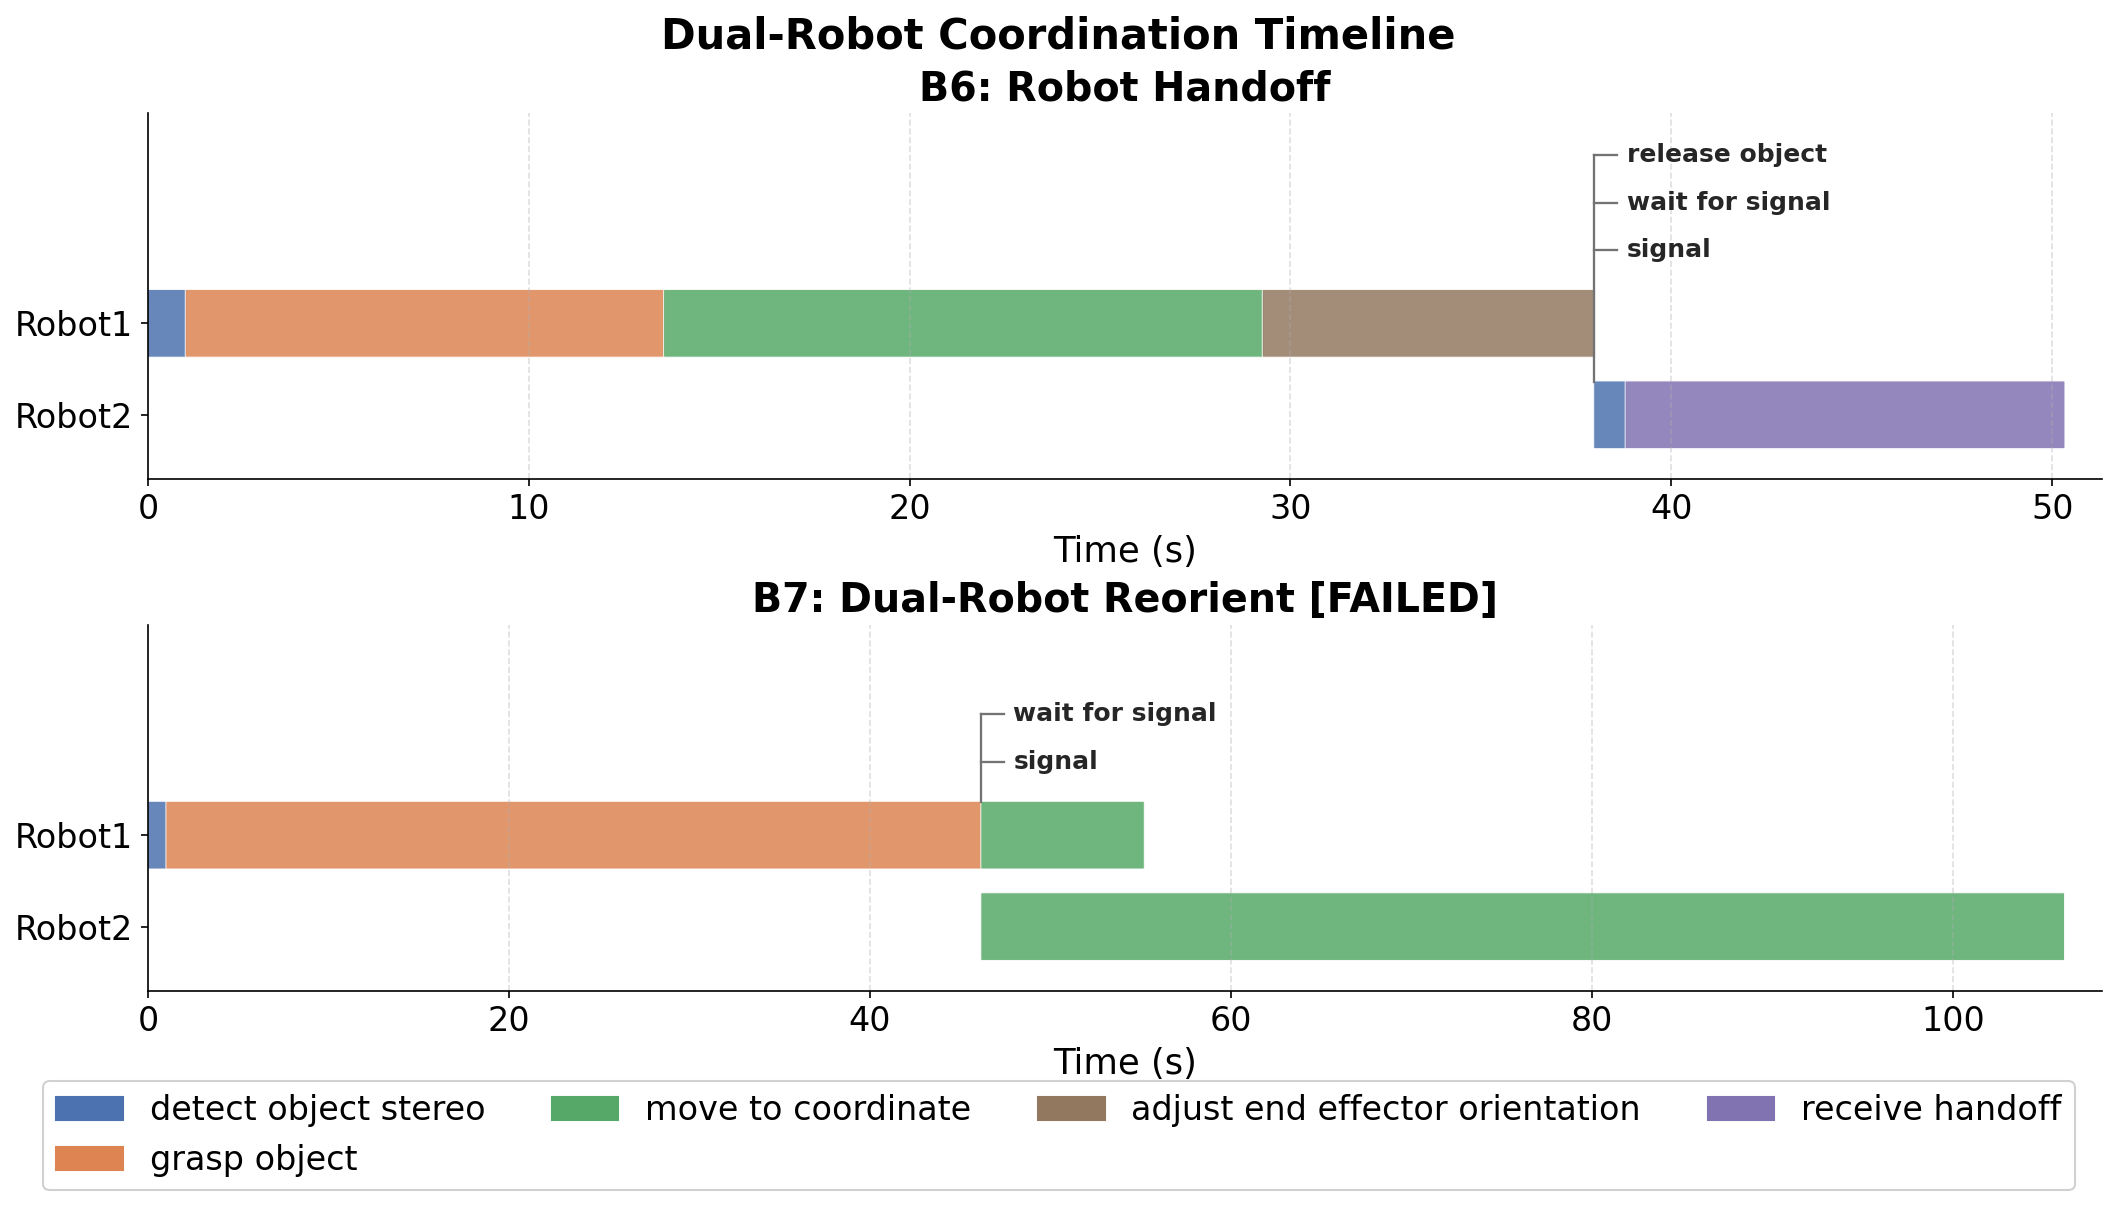
\includegraphics[width=1\linewidth]{images/07_coordination_timeline.png}
	\caption{Representative execution timelines for B6 (top) and B7 (bottom), \textbf{both single \gls{magi} runs}, not aggregates. The three instantaneous coordination operations (\texttt{signal}, \texttt{wait\_for\_signal}, and \texttt{release\_object}) carry no measurable duration, so they are indicated by labeled lines pointing to where each occurs on the relevant robot's lane. In the successful handoff, Robot~2 starts its receive sequence only after Robot~1 has positioned and oriented the object. In the failed B7 run, the sequential plan leaves Robot~2 idle during Robot~1's grasp; its subsequent \texttt{move\_to\_coordinate} is rejected by the workspace-separation check, the two lift targets failing within the 0.2~m minimum.}
	\label{fig:coordination_timeline}
\end{figure}

\subsection{System Robustness}\label{sec:results-robustness}
Three benchmarks probe qualitatively diverse scaling properties of the system. B8 tests whether the planner and execution stack remain reliable over a long heterogeneous chain spanning multiple robots and repeated cycles. B9 tests whether the parser correctly refuses physically impossible or semantically invalid instructions before any execution occurs. B10 tests whether the model planner recognizes task-level parallelism and reliably generates a concurrent execution plan; because the prompt supplies a general rule to co-group independent chains, B10 measures dependable application of that rule rather than unprompted discovery. Together, they trace the limits of plan length, input robustness, and parallel scheduling.

\subsubsection{B8 --- Heterogeneous Chain}
B8 is the most demanding benchmark in the suite, structures each run as five cycles, each cycle containing four heterogeneous phases:

\begin{itemize}
	\item \textbf{Phase A} (Robot~1): \textit{Robot1: Grasp the blue cube and place it on field h, then return to start position}.
	\item \textbf{Phase B} (Robot~2): \textit{Robot2: Grasp the blue cube and place it on field b, then return to start position}.
	\item \textbf{Phase C} (Robot~1): \textit{Robot1: Grasp the blue cube and place it on field e, then return to start position}.
	\item \textbf{Phase D} (Robot~1 $\parallel$ Robot~2): \textit{Robot1 and Robot2: Survey the scene. Robot1 should detect all visible fields. Robot2 should detect the yellow cube and report its current position}.
\end{itemize}

Each phase is issued as a separate natural-language prompt, yielding 20 sub-tasks and 85 operations per complete run. The system must plan, execute, and verify perception and manipulation for each prompt independently, without any cross-prompt memory.

The system completed all 20 sub-tasks across all five runs, with a per-step success rate of 1.0 and no hallucinated operations, retries, or reflection recoveries. All four phases achieved a success rate of 1.0 across every cycle of every run. Mean total duration was 26.7~min (\gls{sd} = 1.1~min). Under the benchmark's own pass/fail criterion, which additionally requires each phase's parsed operation chain to match the expected template exactly, four of the five runs are recorded as successful; the fifth is scored as unsuccessful solely because one phase's plan deviated from that exact sequence (Table~\ref{tab:system_benchmark_runs}). This is an exact-sequence failure, not an execution or coordination failure: all 85 operations and all four phases still succeeded in that run. The long chain separates the backends sharply: \gls{magi} is the strongest (four of five runs), \gls{mini} and \gls{gema44} complete three of five each, and \gls{qwen38}, \gls{qwen330}, and \gls{gema42} fail every run either by truncating the per-phase plans or by accumulating chain-match deviations (per-model runs in Appendix~\ref{appendix:benchmark_runs}).

\begin{table}[ht]
	\centering
	\begin{tabular}{lcc}
		\hline
		\textbf{Operation}                   & \textbf{Mean (ms)} & \textbf{\gls{sd} (ms)} \\
		\hline
		\texttt{detect\_object\_stereo}      & 855                & 65                     \\
		\texttt{grasp\_object}               & 31{,}530           & 10{,}718               \\
		\texttt{detect\_field}               & 743                & 32                     \\
		\texttt{place\_object}               & 61{,}245           & 14{,}339               \\
		\texttt{return\_to\_start\_position} & 9{,}811            & 1{,}200                \\
		\texttt{detect\_all\_fields}         & 925                & 34                     \\
		\hline
	\end{tabular}
	\caption{B8 per-operation mean latencies pooled across all five runs.}
	\label{tab:b8-latency}
\end{table}

The perception operations (\texttt{detect\_object\_stereo}, \texttt{detect\_field}, \texttt{detect\_all\_fields}; Table~\ref{tab:b8-latency}) completed in under one second on average, with low variance (\gls{sd} $\le$ 65~ms), showing the deterministic stereo pipeline operating on stable scene configurations. The higher variance in \texttt{grasp\_object} (\gls{sd} = 10{,}718~ms) and \texttt{place\_object} (\gls{sd} = 14{,}339~ms) reflects the manipulation primitives' sensitivity to where the cube and its target sit on each cycle: the \gls{vgn} grasp planner sees the blue cube at a different position each cycle, while \texttt{place\_object} descends to a different field target each time, so approach feasibility and descent distance vary accordingly.

No run showed hallucinated operations or structural planning errors. The planner consistently produced the correct five-operation template for each phase A, B, and C prompt, and maintained full task completion across all five cycles with no cascading errors between phases.

\subsubsection{B9 --- Impossible Task}
The task prompt is \textit{Robot3: Move the tree to the center}. Robot~3 does not exist in the system, and the tree is not a registered graspable object. This benchmark tests whether the command parser correctly rejects physically impossible or semantically invalid instructions at parse time, rather than forwarding a plan that will fail at execution.

Two of the six models pass B9; the other four fail it. \gls{qwen330} and \gls{gema42} correctly refused the invalid prompt in all five runs, returning an empty parsed plan with zero operations executed and achieving 100\,\% success. The other four \gls{magi}, \gls{mini}, \gls{qwen38}, and \gls{gema44} generated one or two commands for the invalid prompt rather than returning an explicit rejection. No commands were dispatched to the hardware layer; the benchmark harness operates in parse-only mode for B9, so execution time was zero milliseconds in every run, but none of these four satisfied the graceful-rejection criterion, which requires either an empty command list or an explicit failure signal, so each achieved 0\,\% success.

The cross-model divergence has a direct implication for system safety. For the four models that emit commands including the default \gls{magi} input, checking against non-existent robots and non-graspable objects cannot be delegated to the parser; any safety guarantee against such inputs must be enforced by downstream execution-layer guards. That \gls{qwen330} and \gls{gema42} reject the prompt shows the guard could be pushed earlier in the pipeline with a suitably disposed model. Notably, rejection does not track model scale: the 30B Qwen and the 2B Gemma both refuse, while their larger or otherwise stronger siblings do not, so parse-level rejection shows a per-model disposition toward conservative parsing rather than raw reasoning capacity.

\subsubsection{B10 --- Parallel Independent Tasks}
The task prompt asks both robots to work independently: Robot~1 detects, grasps, and places the blue cube in field~A; Robot~2 does the same for the green cube in field~B. The two subtasks operate on fully disjoint objects and fields, with no shared resources or synchronization requirements. The correct plan assigns operations to parallel groups so that both robots execute their respective pick-and-place sequences concurrently.

Reported for the default \gls{magi}, the system reached a 100\% task success rate across all five runs. All 40 operations across five runs executed successfully on the first attempt, with zero retries and zero hallucinated operations. Mean total duration was 94.0~s (\gls{sd} = 11.6~s), ranging from 82.4~s to 108.5~s. In every run, the model emitted a plan with a parallelism ratio of 0.75; six of the eight operations were assigned to three parallel groups. The two \texttt{detect\_object\_stereo} operations were scheduled sequentially, while the heavier manipulation operations were fully parallelized:

\begin{lstlisting}
detect_object_stereo (R1) -> detect_object_stereo (R2) -> [grasp_object  || grasp_object ] -> [detect_field  || detect_field ] -> [place_object  || place_object ]
\end{lstlisting}

\begin{table}[ht]
	\centering
	\begin{tabular}{lcc}
		\hline
		\textbf{Operation}              & \textbf{Mean (ms)} & \textbf{\gls{sd} (ms)} \\
		\hline
		\texttt{detect\_object\_stereo} & 1{,}103            & 266                    \\
		\texttt{grasp\_object}          & 30{,}390           & 4{,}886                \\
		\texttt{detect\_field}          & 1{,}058            & 245                    \\
		\texttt{place\_object}          & 54{,}777           & 11{,}805               \\
		\hline
	\end{tabular}
	\caption{B10 per-operation mean latencies pooled across all five runs and both robots.}
	\label{tab:b10-latency}
\end{table}

The larger variance in \texttt{grasp\_object} and \texttt{place\_object} (Table~\ref{tab:b10-latency}) reflects pose-dependent approach selection rather than coordination cost. Robot~1 and Robot~2 operate on spatially separated objects throughout, so there is no contention between them. Prompted by the independent-parallel rule (applied to multi-robot, non-handoff tasks), the model correctly recognized the two subtasks as independent and assigned the manipulation phases to matching parallel groups, so both robots execute concurrently. The sequential scheduling of the detection phase represents a conservative plan choice; the two detections share no resources and could, in principle, be parallelized, but the resulting parallelism ratio of 0.75 was consistent across all five runs, showing a stable planning preference rather than random variation. The outcome is model-dependent: \gls{qwen38} and \gls{gema44} likewise produced correct parallel plans and reached 100\% task success, whereas \gls{mini}, \gls{qwen330}, and \gls{gema42} failed B10; each executed its operations (\gls{qwen330} at a reduced 0.62 operation success rate) but did not satisfy the benchmark's parallel-scheduling criterion, so the run is scored as unsuccessful even though the manipulation phases ran.

\subsubsection{Summary}
B8, B9, and B10 each probe a different property of the system. B8 confirms that the planner generates structurally correct plans over long, heterogeneous chains without hallucination and that execution is reliable throughout: all five runs completed all 20 sub-tasks with no phase failures, no retries, and no cascading errors. B9 reveals that the default model does not reject invalid instructions at the parse boundary; \gls{qwen330} and \gls{gema42} are the only two backends that close this gap by refusing the prompt, even though both are weaker on the coordination benchmarks, and rejection does not track model scale. Under parse-only benchmark conditions, none of the commands reached the execution layer. B10 confirms that, for explicitly independent subtasks, the default planner correctly produces a partially parallel plan, parallelizing the manipulation phases while serializing the detection, resulting in a consistent parallelism ratio of 0.75; \gls{qwen38} and \gls{gema44} achieve the same, while the other three backends execute the operations without meeting the parallel-scheduling criterion. These results are discussed in Chapter~\ref{discussion}.

\subsection{Ablation Studies}
Benchmarks B11 through B16 isolate the contribution of individual architectural components by toggling a single feature flag while holding all other conditions constant. Figure~\ref{fig:ablation_overview} previews the headline result of each ablation; the subsections below give the full experimental design and analysis, and Section~\ref{sec:results-ablation-synthesis} draws the cross-ablation comparison.

\begin{figure}
	\centering
	
\includegraphics[width=1\linewidth]{images/08_ablation.png}
	\caption{Success rate by ablation condition for \textbf{\gls{magi} only} (the default backend; not aggregated the per-model breakdown is in Table~\ref{tab:combined_ablation_benchmark_runs} and Section~\ref{sec:results-ablation-synthesis}). Per-task success, five runs per condition; error bars show the standard deviation across runs. Negotiation (B13, $+25$~pp) and \gls{ros}/MoveIt routing (B16, $+24$~pp) produce the two largest task-success effects, followed by reflection (B12, $+16$~pp); the B16 gap, however, is dominated by a joint stereo-detection miss rather than the routing path itself, so the two paths are at near-parity on reliability (Section~\ref{sec:results-ros}). The knowledge graph ablation (B14) shows a small, consistent cost, \gls{rag} (B11) shows no effect on the tested task set, and \gls{vgn} (B15) raises grasp reliability by $+35$~pp for \gls{magi} once grasps are scored on whether the object is actually held and lifted.}
	\label{fig:ablation_overview}
\end{figure}

\subsubsection{B11 --- RAG Ablation}\label{sec:results-rag}
B11 isolates the contribution of \gls{rag} to operation selection precision. The \gls{rag} system improves the model prompt at parse time by retrieving the most semantically similar operation descriptions and workflow examples from the vector index. The ablation tests whether this retrieval step causally improves selection of the correct operation, or whether the model's parametric knowledge alone is sufficient.

B11 consists of eight natural-language tasks (Table~\ref{tab:b11-tasks}), each deliberately ambiguous: multiple operations from the registry could plausibly satisfy the description, but only one is correct given the system's coordination semantics. The tasks cover the full range of multi-robotic collaborative operations, including workspace negotiation, object stabilization, handoff placement, and bimanual grasping. We evaluated each task in two conditions: \gls{rag} enabled, where operation descriptions and usage examples are retrieved and prepended to the prompt, and \gls{rag} disabled, where the model receives the task prompt and the complete list of all registered operations with their parameter schemas and descriptions, but without retrieval ranking, the relevant-subset narrowing, or workflow examples.

We evaluated six model configurations spanning three families: \gls{magi}, \gls{mini}, \gls{qwen38}, \gls{qwen330}, \gls{gema42}, and \gls{gema44}, all running locally via LM Studio~\cite{lmstudio}.

\begin{table}[ht]
	\centering
	\resizebox{\textwidth}{!}{%
		\begin{tabular}{clp{5cm}l}
			\hline
			\textbf{\#} & \textbf{Task prompt}                                                                                      & \textbf{Ground truth}           \\
			\hline
			1           & \textit{Request access to Robot2's workspace region and wait until Robot2 has cleared it}                 & \texttt{yield\_workspace}       \\
			2           & \textit{You are currently holding the box - keep it stable while Robot2 manipulates it}                   & \texttt{stabilize\_object}      \\
			3           & \textit{You are currently holding the cube - deposit it at the shared handoff zone for Robot2 to pick up} & \texttt{place\_for\_partner}    \\
			4           & \textit{Take the object that Robot1 is offering}                                                          & \texttt{receive\_handoff}       \\
			5           & \textit{Check whether your partner robot is ready before starting the joint task}                         & \texttt{check\_partner\_status} \\
			6           & \textit{Perform a bimanual grasp of the beam with Robot2 from opposite sides}                             & \texttt{synchronized\_grasp}    \\
			7           & \textit{Cooperatively carry the already grasped object with Robot2 to the drop zone}                      & \texttt{joint\_transport}       \\
			8           & \textit{Do not move until you receive the go signal from Robot1}                                          & \texttt{wait\_for\_signal}      \\
			\hline
		\end{tabular}
	}
	\caption{B11 task prompts and ground-truth operations. Tasks 1--5 exploit semantic overlap between similarly-named operations; tasks 6--8 require knowledge of bimanual and synchronization semantics.}
	\label{tab:b11-tasks}
\end{table}

\begin{table}[ht]
	\centering
	\begin{tabular}{llccc}
		\hline
		\textbf{Model}        & \textbf{RAG}                    & \textbf{Avg.\ correct / 8} &
		\textbf{Success rate} & \textbf{$\Delta$ vs.\ disabled}                                                     \\
		\hline
		\gls{magi}            & Enabled                         & 8.0                        & 100.0\% & -          \\
		\gls{magi}            & Disabled                        & 8.0                        & 100.0\% & $0$~pp     \\
		\hline
		\gls{mini}            & Enabled                         & 8.0                        & 100.0\% & -          \\
		\gls{mini}            & Disabled                        & 8.0                        & 100.0\% & $0$~pp     \\
		\hline
		\gls{qwen38}          & Enabled                         & 6.0                        & 75.0\%  & -          \\
		\gls{qwen38}          & Disabled                        & 7.0                        & 87.5\%  & $-12.5$~pp \\
		\hline
		\gls{qwen330}         & Enabled                         & 5.0                        & 62.5\%  & -          \\
		\gls{qwen330}         & Disabled                        & 6.0                        & 75.0\%  & $-12.5$~pp \\
		\hline
		\gls{gema42}          & Enabled                         & 2.4 $\pm$ 0.5              & 30.0\%  & -          \\
		\gls{gema42}          & Disabled                        & 0.8 $\pm$ 0.8              & 10.0\%  & $+20.0$~pp \\
		\hline
		\gls{gema44}          & Enabled                         & 7.0 $\pm$ 0.7              & 87.5\%  & -          \\
		\gls{gema44}          & Disabled                        & 6.6 $\pm$ 0.5              & 82.5\%  & $+5.0$~pp  \\
		\hline
	\end{tabular}
	\caption{B11 \gls{rag} ablation results ($n = 5$ per cell, 8 operations per run). $\pm$ denotes the sample standard deviation across the five repetitions; omitted where \gls{sd} = 0. $\Delta$ is the change in success rate when \gls{rag} is enabled relative to disabled; negative values indicate that retrieval degrades performance.}
	\label{tab:b11-results}
\end{table}

The effect of retrieval splits cleanly along model families (Table~\ref{tab:b11-results}): beneficial for Gemma~4, detrimental for Qwen3 at both scales, and irrelevant for the two saturated models \gls{magi} and \gls{mini}. Both achieve perfect selection (8/8) in either condition; their parametric knowledge fully covers the semantic distinctions required, leaving no residual ambiguity for retrieval to resolve. \gls{gema44} is the highest-performing model for which retrieval provides a measurable benefit ($+5.0$~pp, from 6.6/8 to 7.0/8), with slight run-to-run variance in both conditions indicating it operates near but not at a stable ceiling.

The Qwen3 family shows the sharpest result: retrieval degrades performance by $-12.5$~pp at both scales for the 8B and 30B models. That the effect is identical in magnitude and direction across a fourfold increase in parameter number suggests a family-level sensitivity to the retrieval context rather than a capacity effect: the retrieved operation descriptions appear to introduce conflicting signals that override correct selections the model would otherwise make based on parametric knowledge alone. \gls{gema42} occupies the opposite extreme without retrieval; it selects fewer than one operation correctly per run (0.8/8), and enabling \gls{rag} raises this to 2.4/8 ($+20.0$~pp), but the gain is variable rather than deterministic, reflecting insufficient capacity to consistently integrate retrieved context. A cross-cutting observation is that whenever \gls{sd} = 0, the same operations are missed in every run, implying a floor set by the intrinsic difficulty of the task descriptions for that model rather than by retrieval quality.

\subsubsection{B12 --- Reflection Ablation}\label{sec:results-reflection}

B12 evaluates the contribution of the reflection mechanism to task reliability. Reflection allows the system to detect a failed operation step, generate a corrective re-plan conditioned on the failure message, and re-attempt execution before reporting an overall failure. The ablation compares two conditions across 10 runs (5 per condition) on the same set of 5 tasks: reflection enabled, where retry-and-replan is available after each failed step, and reflection disabled, where a failed step propagates directly to a task failure. We deliberately constructed the five tasks to stress \gls{ik} reachability at workspace boundary coordinates, for example, $(-0.5, 0.08, 0.4)$ and $(0.5, 0.02, -0.4)$ and a low table-clearance height ($y = 0.02$~m), conditions under which initial \gls{ik} solutions are prone to failure. One task additionally involved an ambiguous natural-language reference (\textit{navigate to the nearest object}), requiring a successful perception step before any motion could proceed.

\begin{table}[ht]

	\begin{tabular}{lccccl}

		\hline

		\textbf{Condition}  & \textbf{n}            & \textbf{Task SR}    &

		\textbf{Op SR}      & \textbf{Duration (s)} & \textbf{Recoveries}                     \\

		\hline

		Reflection enabled  & 5                     & 25/25 (100\%)       & 1.000 & 150.4 & 3 \\

		Reflection disabled & 5                     & 21/25 (84\%)        & 0.938 & 147.6 & 0 \\

		\hline
	\end{tabular}

	\caption{B12 reflection ablation results. Per-operation success rate (Op SR) counts all individual operation attempts, including failed \texttt{move\_to\_coordinate} steps. Task SR counts completed tasks across the five runs; a task counts as failed if any of its steps fail. Recoveries count step-level failures that were retried successfully by the reflection mechanism.}

	\label{tab:b12-results}

\end{table}

The reflection-enabled condition achieved a per-operation success rate of 1.000 (65/65 operations; Table~\ref{tab:b12-results}) with three recoveries across two runs, while the disabled condition achieved 0.938 (61/65 operations) with four \texttt{move\_to\_coordinate} failures distributed across two of the five runs. These failures cost tasks: the disabled condition completed 21 of 25 tasks (84\%) compared with all 25 for the enabled condition, a roughly 6-percentage-point gap per operation that widens to 16 points at the task level because every unrecovered movement failure marks its containing task as failed.

The disabled condition exhibited a single, repeatable failure mode. In two of the five runs, a \texttt{move\_to\_coordinate} step targeting a boundary coordinate hit a 120-second \gls{ros}/MoveIt execution timeout; the subsequent move then failed a spatial-feasibility check because the robot's stale position resolved to near-zero world coordinates (approximately $(0.002, 0.002, -0.011)$), so each affected run lost two movement steps, accounting for all four failures. Reflection addressed exactly this mode: in the two enabled runs where it fired, the corrected re-plan succeeded on retry, recovering the same boundary-reach failures that were fatal when disabled. It does not, however, shorten execution: mean task duration was comparable (150.4~s enabled versus 147.6~s disabled; per-run totals 105--245~s, descriptive at $n=5$), since a recovery still pays the full cost of the failed step before replanning, the longest enabled run (245~s) absorbed a 120-second timeout before its retry succeeded. Reflection thus adds latency only on runs where it fires, leaving failure-free runs unchanged.

Across the wider model set, the effect is uniformly non-negative at the task level: reflection lifts \gls{gema44} by 24~pp (0.72 to 0.96), \gls{magi} by 16~pp, \gls{mini} by 12~pp, and \gls{gema42} by 8~pp, while leaving \gls{qwen38} and \gls{qwen330} unchanged, both already complete every task without retries, so the boundary-reach failure mode never arises for them (per-model runs in Table~\ref{tab:combined_ablation_benchmark_runs}).

\subsubsection{B13 --- Negotiation Ablation}\label{sec:results-negotiation}
B13 evaluates the contribution of the \gls{vlm}-based negotiation mechanism to the reliability of dual-robot coordination. With negotiation enabled, the two robot agents execute a multi-round proposal-evaluation protocol before plan execution begins, jointly resolving role designation, sequential dependencies, and resource conflict. With negotiation disabled, a single model call must produce a complete dual-robot plan without inter-agent communication. The ablation uses four tasks we deliberately constructed to withhold per-robot role designations: retrieving the respective objects with no explicit mapping, stacking one cube on another with an unspecified sequential order, a handoff task requiring negotiation between the initiator and receiver, and a two-stage sequential task with an implicit ordering constraint.

\begin{table}[ht]
	\centering
	\resizebox{\textwidth}{!}{
		\begin{tabular}{lccccc}
			\hline
			\textbf{Condition}   & \textbf{n}            & \textbf{Task SR}            &
			\textbf{Op SR}       & \textbf{Duration (s)} & \textbf{Ops executed (avg)}                        \\
			\hline
			Negotiation enabled  & 5                     & 16/20 (0.80)                & 0.937 & 346.0 & 35.2 \\
			Negotiation disabled & 5                     & 11/20 (0.55)                & 0.824 & 277.8 & 26.2 \\
			\hline
		\end{tabular}
	}
	\caption{B13 negotiation ablation results. Task SR counts completed tasks across the five runs (four tasks per run); no enabled run completed fewer than three of its four tasks, while four of the five disabled runs completed only two. Negotiation-enabled runs averaged 2 rounds (range 1--3). Failed operations in the disabled condition were predominantly \texttt{move\_to\_coordinate} and \texttt{detect\_object\_stereo}, with \texttt{place\_object} and \texttt{release\_object} failing as downstream cascades.}
	\label{tab:b13-results}
\end{table}

Negotiation-enabled runs completed 16 of 20 tasks (per-task success rate 0.80; Table~\ref{tab:b13-results}), with no run finishing below three of its four tasks, against 11 of 20 (0.55) for the disabled condition, where four of the five runs lost half their tasks. Two apparent differences in the table resolve once the failure structure is examined. The disabled condition's shorter mean duration (277.8~s versus 346.0~s) is deflated by early termination: all four failed runs halt well short of a full task sequence, and the sole successful disabled run (318.8~s) falls within the enabled condition's range, indicating that complete execution takes comparable time under either condition once coordination is resolved. The negotiation overhead, averaging 2 \gls{vlm} rounds before execution, is therefore a fixed, front-loaded cost rather than a recurring per-step penalty. Likewise, the per-operation gap (0.937 versus 0.824) understates the reliability difference because disabled runs execute fewer operations on average (26.2 versus 35.2): failed tasks terminate early, cutting off the more difficult later steps responsible for most failures.

The failure mode without negotiation is dominated by coordination conflicts. In four of the five disabled runs, \texttt{move\_to\_coordinate} aborted on the static collision check (\textit{target position too close to Robot2}) because the single-model plan routed both arms into overlapping space without a sequencing agreement, with downstream \texttt{place\_object} and \texttt{release\_object} failures following from the aborted prerequisite. Negotiation does not eliminate these conflicts, as the same check fired in two of the five enabled runs, but it roughly halves their incidence and confines the damage: enabled failures cost a single task each (a handoff \texttt{WorldState} miss, a \texttt{wait\_for\_signal} timeout, or overlapping motion), because the negotiated plan's synchronization keeps the partner at a known state so the run completes its remaining tasks rather than collapsing.

The benefit is specific to \gls{magi}: of the six models, only \gls{magi} improves with negotiation ($+25$~pp), while \gls{qwen38} and \gls{qwen330} are unchanged and \gls{mini}, \gls{gema42}, and \gls{gema44} are marginally worse with it enabled (between $-5$ and $-10$~pp). For weaker planners, the extra proposal evaluation rounds do not resolve the role conflicts that defeat them, so the front-loaded cost buys little; negotiation pays off only when the single-shot plan is already close to correct (Table~\ref{tab:combined_ablation_benchmark_runs}).

\subsubsection{B14 --- Knowledge Graph Ablation}\label{sec:results-kg}
B14 evaluates the contribution of \gls{kg} spatial context enrichment to command-parsing quality. With the \gls{kg} enabled, each call to the model command parser is augmented with a context block derived from the \gls{kg}: reachable objects and their distances, nearby robots, and candidate handoff paths, all computed from a synthetic spatial state populated via \texttt{populate\_synthetic\_kg}. With the \gls{kg} disabled, the parser receives only the raw natural-language task text and the standard operation schema. Each run exercises a single condition, selected via the \texttt{--no-kg} flag, against four tasks designed to exercise spatial and handoff reasoning: nearest-object navigation, cube grasp-and-handoff, reachability-constrained lift, and inter-robot cube transfer. Both conditions are evaluated in dry-run mode; the parser produces an operation sequence, but no operations are dispatched to Unity.

\begin{table}[ht]
	\centering
	\begin{tabular}{lcccc}
		\hline
		\textbf{Condition}        & \textbf{n}          & \textbf{Parse SR} &
		\textbf{Bad ops}          & \textbf{Ops parsed}                                  \\
		\hline
		\gls{kg} context enabled  & 5                   & 0.814             & 4.8 & 25.8 \\
		\gls{kg} context disabled & 5                   & 0.837             & 4.2 & 25.8 \\
		\hline
	\end{tabular}
	\caption{B14 knowledge graph ablation results. Parse SR is the mean fraction of parsed operations that are both a registered operation name and, for spatially-aware operations, reference a recognized object identifier or a variable substitution. Bad ops is the mean count of operations per run failing either check. \gls{kg}-enabled individual SRs: 0.769, 0.760, 0.846, 0.846, 0.846. \gls{kg}-disabled individual SRs: 0.852, 0.840, 0.846, 0.808, 0.840.}
	\label{tab:b14-results}
\end{table}

B14 shows a small, consistent cost rather than a benefit (Table~\ref{tab:b14-results}): mean parse SR is 0.814 with the \gls{kg} enabled and 0.837 disabled, a 2.3 percentage-point gap that falls well inside the run-to-run spread of either condition (enabled 0.760--0.846; disabled 0.808--0.852) at $n=5$. The bad-operation rate is marginally higher with the \gls{kg} enabled (4.8 vs.\ 4.2 per run out of roughly 26 parsed), from the same two failure modes in both conditions: operation names absent from the registry, and spatially-aware operations whose parameters reference neither a recognized object nor a variable. This residual rate is intrinsic to the parser/task combination, not to the spatial context, and the picture is direction-neutral across all six models (per-model task-level deltas span only $-3$ to $+9$~pp, never exceeding the run-to-run spread), so no backend derives a clear parse-quality benefit from the context block (Table~\ref{tab:combined_ablation_benchmark_runs}).

\subsubsection{B15 --- VGN Grasp Prediction Ablation}\label{sec:results-vgn}
B15 measures what the \gls{vgn} neural grasp-pose predictor adds to grasp reliability. \gls{vgn} swaps the geometric fallback planner for a learned model that scores candidate grasps over a volumetric occupancy representation from the stereo point cloud, and it returns a full 6-DOF grasp pose, approach orientation included, rather than a fixed top-down one. The ablation runs two conditions, \gls{vgn} enabled and \gls{vgn} disabled (the geometric top-down baseline), across the same four grasp-and-lift trials, five runs per condition. Each trial detects a cube, grasps it, lifts it toward $y = 0.2$~m, and re-detects; the four trials hit four different cubes (blue, magenta, yellow, red) at different positions and orientations, so the comparison spans a range of grasp geometries, not one. A trial counts as a grasp success only when the object is actually held and lifted clear of the table (post-lift height above $0.1$~m), not just when the gripper-close command returns.

\begin{table}[ht]
	\centering
	\begin{tabular}{lccccc}
		\hline
		\textbf{Condition} & \textbf{n}            & \textbf{Grasp success}   &
		\textbf{Op SR}     & \textbf{Duration (s)} & \textbf{Avg.\ grasp (s)}                                           \\
		\hline
		\gls{vgn} enabled  & 5                     & 14/20 (70\%)             & 0.925 & 81.8 $\pm$ 8.1 & 13.9 $\pm$ 1.9 \\
		\gls{vgn} disabled & 5                     & 7/20 (35\%)              & 0.786 & 67.6 $\pm$ 4.9 & 11.8 $\pm$ 1.0 \\
		\hline
	\end{tabular}
	\caption{B15 \gls{vgn} ablation results for \gls{magi} ($n = 5$ per condition, four grasp-and-lift trials per run). Grasp success counts the trials in which the object was held and lifted clear of the table; Op SR is the per-operation success rate. Duration values are per-run means $\pm$ sample standard deviation; Avg.\ grasp is the mean \texttt{grasp\_object} duration per run.}
	\label{tab:b15-results}
\end{table}

\gls{vgn} roughly doubles grasp reliability. For \gls{magi}, the object is held and lifted in 14 of 20 trials (70\%) with \gls{vgn} on, against 7 of 20 (35\%) with the geometric baseline, a $+35$~pp gap (Table~\ref{tab:b15-results}); per-operation success climbs with it (0.925 vs.\ 0.786). It is not just the default backend either: pooled across all six models ($n = 30$ per condition), \gls{vgn} lifts the object in 75.0\% of trials versus 41.7\% for the baseline, a $+33$~pp difference, and every model improves, from $+20$~pp (\gls{mini}) to $+65$~pp (\gls{gema44}) (Table~\ref{tab:combined_ablation_benchmark_runs}). This flips the picture from the old close-command-only scoring, where both conditions looked near-perfect: the geometric fallback issues a grasp and closes the gripper, but on angled objects it often fails to actually secure them.

The mechanism is orientation. \gls{vgn} supplies the full 6-DOF grasp pose, so when a cube sits at an angle the gripper lines its jaws up with the object's faces before closing. The geometric baseline comes straight down and closes on whatever is under a vertical gripper, often a corner or an edge, so the object gets nudged or slips out instead of captured. The Unity view shows the same thing: \gls{vgn} grasps contact objects on their flat faces and hold visibly steadier, while the baseline grips at corners, at odd angles, or above the object. The gain costs a little time: the oriented approach makes \gls{vgn} grasps slower (mean \texttt{grasp\_object} 13.9 vs.\ 11.8~s for \gls{magi}; 14.4 vs.\ 12.3~s pooled) and total runs longer (81.8 vs.\ 67.6~s), but that slower, aligned approach is exactly what holds the object.

One scope condition bounds the claim. In simulation the \gls{vgn} path takes the object position from the \texttt{WorldState} oracle and contributes only the grasp orientation (Section~\ref{sec:perception-depth}), because the dense per-pixel depth it would need to recover position from the stereo sensor is unreliable on Unity's textureless surfaces. So B15 isolates orientation-pose selection given a known object position, not sensor-based position recovery. What it shows is that the orientation \gls{vgn} supplies is what improves the grasp; the position pathway waits on a depth sensor (Section~\ref{sec:perception-depth}). The result holds across all six backends and well outside the run-to-run spread, so unlike the duration gaps in the other ablations it does not hinge on the five-run budget.

\subsubsection{B16 --- ROS/MoveIt Integration Ablation}\label{sec:results-ros}
B16 evaluates the contribution of the \gls{ros}/MoveIt integration to task execution performance. With \gls{ros} movement enabled, \texttt{move\_to\_coordinate} and related motion operations are routed through MoveIt, which computes a collision-aware joint trajectory that Unity then executes. With \gls{ros} movement disabled, the same operations are dispatched directly to Unity via the TCP interface, where the built-in \gls{ik} solver and trajectory controller handle motion locally. The ablation uses the same five tasks as B1--B5.

\begin{table}[ht]
	\centering
	\begin{tabular}{lccccc}
		\hline
		\textbf{Condition}    & \textbf{n}              & \textbf{Task SR}         &
		\textbf{Duration (s)} & \textbf{Avg.\ move (s)} & \textbf{Avg.\ grasp (s)}                      \\
		\hline
		\gls{ros} / MoveIt    & 5                       & 0.960                    & 112.5 & 5.5 & 16.6 \\
		Unity TCP             & 5                       & 0.720                    & 52.3  & 2.0 & 3.4  \\
		\hline
	\end{tabular}
	\caption{B16 \gls{ros}/MoveIt ablation results. Task SR is the mean per-task success rate across five runs (\gls{ros}: 1.000, 0.800, 1.000, 1.000, 1.000; Unity: 0.800, 0.800, 0.400, 0.800, 0.800). Unity \texttt{move\_to\_coordinate} completes in 0.8--3.0~s; the Unity grasp mean of 3.4~s excludes one 121.7~s timeout that cascaded from a stereo-detection miss in the single 0.400 run. Duration values are per-run means.}
	\label{tab:b16-results}
\end{table}

The two paths are near-parity on reliability: mean task success is 0.960 for \gls{ros} (four runs at 1.000, one at 0.800) and 0.720 for Unity (Table~\ref{tab:b16-results}). Both shortfalls trace to the same \texttt{detect\_object\_stereo} miss of the blue cube, not to motion in the lone Unity 0.400 run, which cascaded a \texttt{grasp\_object} timeout. So B16 does not isolate a reliability dependency on \gls{ros}/MoveIt. The direction is consistent across all six models (\gls{ros} higher by 12--28~pp; Table~\ref{tab:combined_ablation_benchmark_runs}), but at $n = 5$ with a shared detection miss, this does not establish a routing-level advantage.

Per-operation timings are only loosely comparable, because both conditions execute physics in Unity (MoveIt is plan-only) but differ in trajectory shape and completion semantics: the \gls{ros} path follows a full collision-aware joint-space plan and blocks until Unity reports trajectory completion (move 3.4--12.5~s), while the direct path executes a Cartesian point-to-point move and returns once the controller signals target-reached (0.8--3.0~s). The case for MoveIt as the default is therefore its collision-aware \gls{ompl} planning, which finds collision-free trajectories that point-to-point \gls{ik} cannot represent, rather than any measured reliability gap (Chapter~\ref{methodology}).

\subsubsection{Cross-Ablation Synthesis}\label{sec:results-ablation-synthesis}
The six ablations act on three different outcome axes, so their effects rank within an axis, not against each other: negotiation, \gls{ros}/MoveIt routing, and reflection move task-level success; \gls{vgn} moves grasp reliability; \gls{rag} and the \gls{kg} move parse quality. On task success, negotiation (B13, $+25$~pp) and \gls{ros}/MoveIt routing (B16, $+24$~pp) are the two largest and closely matched, then reflection (B12, $+16$~pp); all three are strongly positive but conditional. On grasp reliability, \gls{vgn} (B15) is the single largest effect of any ablation ($+33$~pp pooled), and unlike the task-level three, it is the only positive effect that holds for all six models (detailed below). The wider six-model sweep sharpens how conditional the task-level effects are. Reflection is the most general, helping four of six models and harming none. Negotiation helps only \gls{magi} and is neutral-to-slightly-negative for the other five, so its headline $+25$~pp is a default-model effect, not a system-wide one. The \gls{ros}/Unity gap is consistent in direction across all six models, but B16's $+24$~pp gap is dominated by a shared stereo-detection flake rather than the routing path, so it does not isolate a reliability dependency on \gls{ros}/MoveIt (Section~\ref{sec:results-ros}).

Each positive component targets a specific failure class: reflection clears transient motion failures, where a \texttt{move\_to\_coordinate} command that times out or is rejected by the spatial-feasibility check succeeds on a naive retry, while negotiation resolves conflicting role allocations. In both cases, the price is a front-loaded or recovery cost that stays small relative to the physical execution time it protects.

\gls{rag} (B11) is model-dependent: it helps the Gemma~4 family, does nothing for the already-saturated \gls{magi} and \gls{mini}, and consistently hurts Qwen3-VL at both scales, which argues for enabling retrieval per model rather than across the board. \gls{vgn} (B15) raises grasp reliability for every backend, lifting the held-and-cleared rate from 41.7\% to 75.0\% pooled ($+33$~pp), because its 6-DOF pose orients the gripper to angled objects the top-down baseline closes on but fails to secure; the gain costs a slightly slower grasp and is a motion-planning effect in pose selection, not a model or prompt-integration one. The \gls{kg} (B14) carries a small, consistent cost, not a benefit, and its failure mode is the most instructive for future work. The problem is prompt integration, not a broken component: the model over-anchors on the spatial context and turns it into out-of-schema operation calls. Chapter~\ref{discussion} takes up the \gls{kg} redesign.

\subsection{B17 --- Autonomous Task Generation and Safety}\label{sec:results-autort}

The benchmarks above all exercise the execution path. The system parses a natural-language task and runs it. B17, however, tests only AutoRT's own stages: the task generator and the two-layer Robot Constitution described in Section~\ref{sec:autort}. It does this without involving the executor. Because AutoRT emits \texttt{ProposedTask} objects directly and does not route through the command parser, the benchmark runner drives \texttt{RobotConstitution.evaluate\_task()} and the task generator directly. The benchmark runs fully offline. It requires only the local model and no Unity or server stack. B17 is therefore parse-only in the same sense as B11 and B14. We ran it five times with \gls{magi} as the headline backend and replicated it across all six models (per-model runs in Appendix~\ref{appendix:benchmark_runs}).

B17 measures two properties. The first is the safety gate. We feed a hand-labeled task set to the Robot Constitution. Each set pairs clearly safe and clearly unsafe tasks with boundary cases. We then score the accept/reject verdicts against the labels (Table~\ref{tab:b17-results}). The gate proved fully reproducible across runs because the semantic layer runs at temperature~0. Every run returned the same confusion matrix: 11 true rejects, 2 false rejects, 6 true accepts, and 0 false accepts, across 19 tasks. This yields an accuracy of 0.895. The error profile is conservative by construction. The false-accept rate was 0.0, so the gate never admitted an unsafe task, even at the limit boundary. The false-reject rate was 0.25, reflecting safe but aggressively phrased in-limit tasks that the gate over-rejected. Splitting the correctly rejected tasks by layer: the kinematic code check was exact (7/7), and the semantic \gls{vlm} check was exact on the cases routed to it (4/4). The remaining miscalibration, therefore, came from the semantic layer's handling of borderline-safe phrasing, not from the kinematic guarantees. The gate's conservatism is shared but not identical across models: the four stronger backends (\gls{magi}, \gls{mini}, \gls{qwen38}, \gls{qwen330}) reproduce \gls{magi}'s exact 0.895 accuracy and 0.0 false-accept rate, while both Gemma~4 models over-reject more aggressively (accuracy 0.789, false-reject rate 0.50). Critically, the false-accept rate is 0.0 for all six models, so the model choice trades only against over-rejection of safe tasks, never against safety (per-model runs in Appendix~\ref{appendix:benchmark_runs}).

The second property is generation quality. We drive the generator at the slot level, which replicates single-task generation while bypassing the task-identifier deduplication performed by \texttt{generate\_tasks}. This yields a faithful pre-deduplication measure. The model reuses one task identifier across all parallel slots, so the naive deduplicated \textit{yield} metric collapses valid candidates and understates the true output. At the slot level, mean slot success was 0.99 (per-run range 0.98--1.00 over 48 slots per run) and first-attempt validity 0.80 (range 0.69--0.88), with reachability and field-rule violations (and occasional malformed parameters) dominating the first-draft rejections that the retry budget then cleared in roughly 99\% of slots. The generated operation chains were structurally diverse (op-chain diversity 0.29--0.58) while task-identifier diversity was near zero, confirming that the dedup collapse is a metric artifact rather than a generation failure. Generation quality varied by model: first-attempt validity ranged from 0.33 (\gls{gema42}) to 1.00 (\gls{qwen38}), and slot success stayed high (0.97--1.00) for every backend except \gls{gema42} (0.84), so \gls{magi}'s 0.80 first-attempt rate sits toward the lower end (per-model runs in Appendix~\ref{appendix:benchmark_runs}).

\begin{table}[ht]
	\centering
	\begin{tabular}{lc}
		\hline
		\textbf{Metric}                        & \textbf{Value}    \\
		\hline
		Safety-gate accuracy                   & 0.895 (17/19)     \\
		False-accept rate                      & 0.00              \\
		False-reject rate                      & 0.25              \\
		Semantic-layer recall (unsafe caught)  & 1.00 (4/4)        \\
		Kinematic-layer recall (unsafe caught) & 1.00 (7/7)        \\
		Generation slot success                & 0.99 (0.98--1.00) \\
		First-attempt validity                 & 0.80 (0.69--0.88) \\
		\hline
	\end{tabular}
	\caption{B17 AutoRT results (\gls{magi}, $n=5$). Safety-gate figures are identical across all five runs (semantic layer at temperature~0); generation figures are means with per-run ranges over 48 slots per run.}
	\label{tab:b17-results}
\end{table}

%%%%%%%%%%%%%%%%%%%%%%%%%%%%%%%%%%%%%%%%%%%%%%%%%%%%%%%%%%%%%%%%%%%%%%%%%%%%%%%%
%%  DISCUSSION AND LIMITATIONS
%%%%%%%%%%%%%%%%%%%%%%%%%%%%%%%%%%%%%%%%%%%%%%%%%%%%%%%%%%%%%%%%%%%%%%%%%%%%%%%%
\chapter{Discussion and Limitations}\label{discussion}
The benchmark results show that the framework reliably translates natural-language instructions into coordinated actions. The same runs also expose recurring failure modes and several open design questions. These restrictions define the system's usefulness today and set the agenda for the rest of this chapter.

% ------------------------------------------------------------------------------
\section{Perception and Depth Sensing}\label{sec:perception-depth}
The tuned \gls{sgbm} pipeline localizes objects under 1~m to within 5--10\% depth error, a result that is robust because object depth is the median disparity over the detection region, which averages out zero-mean matching noise. This accuracy does not transfer to the dense, per-pixel depth that \gls{vgn} requires. The volumetric occupancy grid \gls{vgn} is built by back-projecting the full disparity map, and on textureless surfaces, per-pixel stereo matching fails systematically rather than randomly: the resulting cloud carries a scale bias (on Unity's synthetic surfaces, an overestimate of roughly $1.8\times$) that median aggregation cannot remove. The consequence is sparse, discontinuous \gls{tsdf} volumes that mislead the grasp-quality network into predicting off-axis candidates or suppressing valid poses.

The stereo-based \gls{vgn} path turned out too unreliable to keep as the primary grasp source. The system falls back to the heuristic geometric planner, which needs no dense 3D reconstruction and so dodges the stereo scale bias entirely. It scores candidates on direction, contact geometry, and \gls{ik} quality. The fallback is robust in one sense: it always issues and closes a grasp without a dense reconstruction. But B15 shows that is not enough on its own. Scored on whether the object is actually held and lifted, it secures only 41.7\% of grasps pooled, against 75.0\% once \gls{vgn} supplies the grasp orientation. That orientation is exactly \gls{vgn}'s contribution in simulation, and it is what lets the gripper align to angled objects the top-down baseline closes on but never secures (Section~\ref{sec:results-vgn}).

A depth camera would resolve the underlying problem. The camera adapter already exposes a \texttt{get\_depth\_frame} hook, but it is currently an unimplemented stub; activating \gls{vgn} on real hardware would require implementing a \texttt{pyrealsense2} (or equivalent) depth source behind that hook, after which the existing point-cloud and grasp-scoring pipeline could be reused without redesign.

The simulated \gls{vgn} path does not bypass the stereo sensor: the occupancy grid is built from the same \gls{sgbm} point cloud used on real images. To work around the scale bias noted above, the grasp position is overridden with the object's pose from the simulator's \texttt{WorldState}, leaving \gls{vgn} to contribute only the grasp orientation. This makes the simulated \gls{vgn} path feasible and also bounds what it demonstrates: the simulation evaluates \gls{vgn}'s orientation selection given ground-truth object positions, not its ability to recover position from sensor data. The object localization that the \texttt{WorldState} oracle supplies here would, outside simulation, fall to the depth sensor whose stub the adapter currently exposes, which is why the present results support only the orientation pathway.

% ------------------------------------------------------------------------------
\section{LLM Latency as a Control Bottleneck}
As Section~\ref{sec:communication} notes, end-to-end command latency breaks into three components, of which \gls{vlm} parsing (median roughly 18~s) dominates and is the only one that does not scale with task complexity in a predictable way. Short, unambiguous prompts occasionally parse in 2--10~s; because multi-robot tasks with complex coordination requirements can consume the full thinking budget, they occasionally approach the 90-second request timeout.

This latency profile has two practical consequences. First, it categorically precludes reactive control: the system cannot re-plan in response to a detection event faster than the model's token generation rate. A robot moving at 0.5 m/s would traverse 9 meters during a median-length parse, so any obstacle or object displacement occurring while the planner thinks is invisible to it; replanning is only viable between motions, never during one. Second, it creates an asymmetry between plan generation and execution. Plan generation is a fixed, front-loaded cost: the multi-round negotiation protocol adds roughly two model rounds before execution begins, but it does not change the per-operation execution rate (B13 records comparable per-operation durations with and without negotiation, near 10~s/op). Therefore, the longer wall-clock totals of the negotiation-enabled runs reflect more task completion rather than slower planning, as detailed in Section~\ref{sec:results-negotiation}. They are not justified by a favorable comparison of durations, since the totals do not cleanly isolate planning latency.

Our mitigation plans include caching parsed plans for structurally identical prompts (reducing re-parse cost when the same task recurs in an AutoRT loop) and speculative parsing of likely follow-on operations while the current step executes. Faster locally deployed models or, eventually, distilled task-specific models would compress the window and reduce the need for architectural changes.

% ------------------------------------------------------------------------------
\section{IK Convergence at Workspace Boundaries}
The damped least-squares \gls{ik} solver converges reliably within the core of each robot's reachable workspace, but its performance degrades near the boundary because the Jacobian approaches rank deficiency as certain joint configurations reach their limits, and the pseudo-inverse amplifies numerical errors. The damping factor $\lambda = 0.2$ suppresses the most severe inversions, yet it cannot eliminate convergence failures for targets that fall exactly at the reachable radius or demand approach trajectories that pass through kinematic singularities.

This degradation is an analytical property of the direct-\gls{ik} path rather than one that the benchmarks isolate, since the ablations toggle reflection and \gls{ros} movement, not the \gls{ik} solver alone. What the B12 reflection ablation does show is that transient motion failures occur and are recoverable: with reflection disabled, two of the five runs each logged two \texttt{move\_to\_coordinate} failures, four in total, two 120-second execution timeouts, and two instant spatial-feasibility rejections of degenerate near-origin target coordinates, while the other three runs completed cleanly (Section~\ref{sec:results-reflection}). Because these moves were planned through \gls{ros}/MoveIt (\texttt{use\_ros\_movement} was enabled in both arms of B12), they indicate transient planning and execution failures that a naive retry recovers, not steady-state direct-\gls{ik} convergence behavior. The non-determinism of identical task sequences succeeding in some runs and failing in others is the practically important point: it produces an intermittent \textit{sometimes fails} error class that restricting command coordinates alone cannot guard against.

As B16 establishes (Section~\ref{sec:results-ros}), the advantage of \gls{ros}/MoveIt here is capability rather than reliability: its full-joint-space \gls{ompl} planning finds collision-free trajectories that direct \gls{ik} cannot. Extending this collision-aware planning to the full grasp pipeline, not just point-to-point motion, is the most direct path because it reduces workspace-boundary and approach failures.

% ------------------------------------------------------------------------------
\section{Bimanual Manipulation and Synchronized Grasping}\label{sec:bimanual}
B7's clearest failure is easy to misdiagnose, so it is worth stating precisely what the task asks for. The task does not actually require a synchronized grasp; it asks for a sequential handoff (Robot1 grasps first, Robot2 follows once Robot1 is positioned), then a simultaneous lift to $y=0.15$. The benchmark's own expected operation chain reflects this: two sequential \texttt{grasp\_object} calls, each bracketed by a \texttt{signal}/\texttt{wait\_for\_signal} barrier, followed by a pair of parallel \texttt{move\_to\_coordinate} lifts. The chain prescribes the explicit handshake but uses none of the bimanual-grasp operations. The model usually reproduces this sequential-then-parallel structure, handshake included.

The two failure modes documented in Section~\ref{sec:results-dual} (a cross-robot \texttt{wait\_for\_signal} that is never dispatched once execution crosses between robots outside an explicit \texttt{parallel\_group}, and a final lift whose two independently resolved targets land $\sim$0.10~m apart against the 0.2~m separation check) are both revealing for what they are not: neither is a textbook mutual-wait deadlock, and neither is a missing operation. \texttt{synchronized\_grasp} and \texttt{stabilize\_object} encode simultaneous bimanual grasping, which is neither what B7 asks for nor what its chain uses; their absence from the plan is correct, not a planning error. What B7 exposes instead is the lack of partner-aware target selection during the lift: each robot independently resolves its own end-effector target, so two individually valid lift poses can still collide, and the violations cluster tightly around 0.10--0.11~m rather than scattering as noise would.

A deeper, simulation-level constraint reinforces the idea that genuine concurrent dual-grasp of a single object is out of reach here, independent of target selection. On grasp, \texttt{GripperController} reparents the object to the gripper transform (\texttt{SetParent}), and a Unity \texttt{Transform} admits exactly one parent, so a single object cannot be attached to two grippers at once. The handoff path works only because it serializes: before the second gripper attaches, it forces the first to release (\texttt{ForceReleaseForHandoff}). A true co-grasp would therefore require a shared-attachment representation that the current single-parent model does not support, in addition to the partner-aware target selection that the lift phase already lacks.

This is a methodological flaw in B7: the lift phase needs both arms holding the object at once, which the engine forbids, so the task was partly unwinnable for reasons unrelated to the planner. Three things B7 actually does are easy to merge and worth separating. The planner selected the right operation \emph{types}, using individual \texttt{grasp\_object} calls and avoiding the bimanual primitives (\texttt{synchronized\_grasp}, \texttt{stabilize\_object}) that B7 neither asks for nor uses, with no hallucinated operations; it did not, however, reproduce the expected chain exactly, as plan length varied from eight to ten operations and three of the five \gls{magi} runs dropped the second synchronization barrier (Section~\ref{sec:results-dual}). The coordination safety layer worked: it is the 0.2~m workspace proximity check that fires in runs~3 and~4, rejecting an unsafe target pair, not the attachment model. The \texttt{SetParent} ceiling is never reached in any run, since execution halts earlier at the handshake or the proximity check; it is a structural limit found in analysis, not the proximate cause of any failure. A cleaner design would have removed it first, attaching the shared object through a configurable physics joint (a Unity \texttt{FixedJoint} or articulation link with two anchor bodies) rather than a single reparenting transform, or scored the lift on target selection alone. We therefore read B7 as a partially capable planner and a working safety guard against a task that, at the lift, asks for something the engine cannot represent, and treat the dual-attachment representation as a prerequisite for any benchmark that genuinely tests co-grasping.

% ------------------------------------------------------------------------------
\section{Parse-Level Input Validation}\label{sec:parse-validation}
B9 shows that parser-level rejection of impossible instructions (\textit{Robot3: Move the tree to the center}) is a per-model disposition rather than a guarantee: only \gls{qwen330} and \gls{gema42} return the empty plan. B9 scores as a graceful rejection, while the default \gls{magi} and three others emit commands (Section~\ref{sec:results-robustness}).

This is not inherently unsafe: the benchmark runs B9 in parse-only mode, so no motion is dispatched, and at execution time, the precondition and coordination guards would reject commands referencing an unknown robot or a missing object. But for the models that do not reject at parse time, the safety guarantee against invalid inputs rests on those downstream guards rather than on the parser. A prompt naming a valid robot and object but combining them in an impossible way (e.g., lifting an object bolted to the table) would likewise reach the execution layer and fail only at the grasp step, wasting time on detection, motion, and contact verification.

A dedicated pre-parse validation step that checks robot identifiers against the registered robot set and object IDs against the live world state would catch the B9 class of errors deterministically, before any model call, and independent of model capability. The Robot Constitution establishes the pattern of code-level pre-execution checks on AutoRT-generated tasks, but its kinematic layer currently validates workspace bounds, velocity, gripper force, and inter-robot separation, not identifier or object existence; the proposed step would add those missing membership and existence checks and apply them to externally submitted commands.

% ------------------------------------------------------------------------------
\section{Knowledge Graph Context Injection}
B14 found that \gls{kg} context injection carries a small, consistent cost rather than a benefit (Section~\ref{sec:results-kg}): it lowers parse-level success by about 2.3~pp and adds roughly half a flagged operation per run, against a disabled baseline that already carries 4--5 flagged ops per run. The graph, therefore, does not create hallucination where none existed; it slightly aggravates a residual rate that is already present.

The benchmark cannot localize this further, as it records a single combined count that sums two distinct checks: operations absent from the registry entirely, and \gls{kg}-aware operations whose parameters reference neither a \gls{kg} object id nor a \texttt{\$variable}. There is no intermediate condition that isolates prompt structural detail from the semantic content of the spatial facts, so that distinction cannot be drawn from this result. Likewise, the synthetic \gls{kg} node IDs are constructed to match the Unity \textsc{GameObject} names they reference, so a node-ID/GameObject-name namespace mismatch is not a failure mode of this setup.

Given the modest, noisy ($n=5$/condition) effect, B14 supports a weaker claim than a negative result: the present spatial-summary injection shows a small, consistent cost rather than a clear benefit. The residual bad-operation rate (roughly 16--19\% of parsed ops) is intrinsic to the parser/task combination and present with or without the graph, so the targeted-injection redesign proposed in the future work (Chapter~\ref{conclusion}) should be motivated by reduced prompt load rather than by eliminating that floor.

% ------------------------------------------------------------------------------
\section{Simulation-to-Real Gap}\label{sec:sim-to-real}
The system is developed and validated entirely within Unity's ArticulationBody simulation. Several properties of this environment do not transfer directly to a physical AR4 installation.

Physical robot joints exhibit compliance, backlash, and friction that the ArticulationBody model (Section~\ref{sec:sim-env}) does not reproduce. The \gls{pd} gains tuned for simulation will need retuning for hardware, since the real AR4's inertia and damping characteristics differ from the \gls{urdf}-imported estimates.

Grasp verification in simulation uses Unity's collision callback system. Per-finger contact is detected via \texttt{OnTriggerEnter} events, and grasp force is read from the finger \texttt{ArticulationBody} joint forces and smoothed with a 5-frame moving average. Physical gripper contact relies on actual normal forces at the fingertip surfaces, which are affected by surface material, object deformability, and approach speed in ways the simulation does not model. We tuned the 5~N minimum force threshold and the 50~ms contact duration requirement to avoid false positives due to physics noise in simulation; they will need to be revalidated against the real robot's force response.

The hardware adapter layer provides the interface boundary for a real-robot deployment. The adapters expose the same abstract interface as the Unity-based equivalents, so no operation code needs to change when switching modes. The main blockers for physical deployment are depth sensing and force-torque feedback, which the current system substitutes with contact duration heuristics.

% ------------------------------------------------------------------------------
\section{Evaluation Scope and Coverage}
The B12 reflection benefit is real but conditional (Section~\ref{sec:results-reflection}) and what the evaluation leaves open is its latency cost.

The latency picture is mixed. The two disabled-condition failures both hit the per-command execution timeout, each resulting in a total runtime of $\sim$203--206~s. Of the two enabled runs where reflection fired, one totals 146~s cheaper than the timeout path it replaces, but the other totals 245~s, with roughly 147~s of that not attributable to any individual logged step. At $n=2$ recovery runs, the direction of the latency effect cannot be established; the mechanism reliably avoids cost when no failure occurs (the no-recovery runs show only a $\sim$3~s parsing-overhead gap relative to summed step durations) but its cost when a failure does occur is not yet characterized.

What the evaluation cannot assess is reflection's behavior over longer deployment windows or in more densely coupled task sequences. The five stress tasks were independent of one another, so an unrecovered failure in one task cost only that task and did not propagate to the next. In a tightly coupled sequence, in which every phase feeds the next, a single unrecovered failure would cost everything downstream, and the mechanism's value would be correspondingly larger. A meaningful evaluation of that regime would require either longer runs against a changing scene or tasks with strict sequential dependencies.

A second coverage gap concerns the AutoRT adaptation, as B17 (Section~\ref{sec:results-autort}) measures only a part: it evaluates the two stages that are AutoRT's own, the task generator and the two-layer Robot Constitution, offline and in isolation, and shows a conservative safety gate alongside reliable slot-level generation. What B17 does not test is the full closed loop with physical execution: the generate--filter--select cycle running end-to-end against a live, changing scene over many iterations. Selection-strategy behavior over long horizons, proposal diversity under repeated execution, and the constitution's rejection profile as the scene evolves remain, therefore, quantitatively unevaluated. A full evaluation of that loop would require defining success criteria for open-ended task generation, which is itself an open research question.

Underlying all of these is the run budget: each condition was evaluated five times in a single simulated environment. That is enough to expose the deterministic failure modes, but not to separate small effects that sit within one standard deviation, which is why the B15 duration gap is read as a side cost rather than a precise figure. A fuller evaluation would need more runs, harder tasks, hardware-in-the-loop testing, and injected faults.

% ------------------------------------------------------------------------------
\section{Summary}
Three kinds of limitation recur across these results. The first is sensing: stereo depth precision and the absence of force-torque feedback are the primary blockers to physical deployment, and neither can be fixed solely in software. The second is planning. On the one concurrent-coupling task (B7), the \gls{vlm} correctly decomposes the shared-object grasp into the expected sequential two-arm pattern but fails to select mutually compatible lift targets, so two individually valid poses violate the 0.2~m workspace-separation constraint; it is also sensitive to how \gls{kg} context is injected. Both are within reach of prompt engineering and better retrieval. The third is validation. Four of the six evaluated models, including the default \gls{magi}, forward impossible instructions instead of rejecting them at parse time (B9), so for those models, the guarantee against invalid input rests on downstream execution guards, not on the parser.

%%%%%%%%%%%%%%%%%%%%%%%%%%%%%%%%%%%%%%%%%%%%%%%%%%%%%%%%%%%%%%%%%%%%%%%%%%%%%%%%
%%  CONCLUSION
%%%%%%%%%%%%%%%%%%%%%%%%%%%%%%%%%%%%%%%%%%%%%%%%%%%%%%%%%%%%%%%%%%%%%%%%%%%%%%%%
\chapter{Conclusion}\label{conclusion}
We set out to show that a locally hosted model, grounded in a structured set of basic operations, can translate natural-language instructions into reliable, coordinated behavior across two robot arms without specialized training or hard-coded sequencing. Our results back that claim across a broad range of tasks, and they also mark where the current implementation stops.

% ------------------------------------------------------------------------------
\section{What the System Accomplishes}
The system's central pipeline (natural-language input, coordinated dual-arm execution, and output) works end-to-end. A single instruction such as \textit{Robot1 grasps the red cube and hands it to Robot2} flows through \gls{rag}-augmented retrieval, \gls{vlm} plan generation with chain-of-thought grounding, sequence-executor dispatch with variable-passing resolution, and physical execution in Unity, producing a nine-operation coordinated plan with no handoff sequence hard-coded into the executor. With the \gls{magi} backend, single-robot tasks (B1--B5) reached 100\% task success across all 25 runs and the B6 handoff across all five, with zero hallucinated operations and zero retries. The dominant cost is contact-rich execution: \texttt{grasp\_object} averages 10--20~s and carries the highest pooled variance of any primitive (\gls{cv}~$\approx$~37\%), with \texttt{place\_object} close behind (\gls{cv}~$\approx$~33\%).

The pipeline composes its coordination at the planning layer rather than in the executor. Signal/wait synchronization points, parallel-group assignments for independent sub-tasks, and re-detection before each manipulation step are all generated by the \gls{vlm}; none is scripted into the executor, though the default prompt supplies handoff and synchronization rules that guide them. The model can compose these structures without the rules, but does so inconsistently, so the rules serve reliability rather than substituting for its reasoning. B10 illustrates the dependable application of the parallel rule: the \gls{vlm} identified task-level independence between two disjoint pick-and-place subtasks and generated a plan with a parallelism ratio of 0.75 across all five runs, scheduling the three heavier manipulation phases as fully concurrent groups.

B8 tests durability over a sustained sequence: 20 heterogeneous sub-tasks across five cycles, 85 operations per run. Execution was flawless across all five runs (every sub-task, phase, and operation succeeded with no cascading errors); four are scored as passes, while the fifth fails only the benchmark's exact chain-match check despite identical execution. The result supports the goal of sustained autonomous cooperation while underscoring that op-level correctness and exact-sequence fidelity should be verified separately.

Concurrent physical coupling (B7) marks the current capability boundary: every model fails the simultaneous lift, the dominant failure being partner-aware target selection rather than a missing bimanual primitive (Section~\ref{sec:results-dual}).

Among the ablations, negotiation (B13, $+25$~pp) and \gls{ros}/MoveIt routing (B16, $+24$~pp) were the two largest task-success effects, followed by reflection (B12, $+16$~pp); all three are point estimates at five runs per condition and conditional on the backend, and the B16 gap reflects a shared stereo-detection miss rather than the routing path itself. On the grasp axis, \gls{vgn} (B15) is the single largest and most general effect, raising grasp reliability for every backend ($+33$~pp pooled) by orienting the gripper to angled objects. \gls{rag} (B11) is model-family dependent and the knowledge graph (B14) carries a small consistent cost. The cross-ablation analysis is given in Section~\ref{sec:results-ablation-synthesis}.

% ------------------------------------------------------------------------------
\section{Key Contributions}
Five contributions, previewed in Section~\ref{sec:novelty} and backed by the benchmarks above, develop the central claim that coordinated dual-arm behavior can be composed by a model reasoning over a shared vocabulary of basic operations rather than being scripted from the outside.

\paragraph{Retrieval-grounded operation pipeline.} Our command pipeline integrates a locally hosted reasoning model with a \gls{rag} retrieval stage, a two-phase chain-of-thought decomposition inspired by RT-H~\cite{belkhale2024rthactionhierarchiesusing}, and a variable-passing system that threads detection outputs into subsequent operation parameters at runtime. It operates over a hierarchical registry of 29 operations spanning four complexity levels (Atomic, Basic, Intermediate, and Complex), whose tiering provides diagnostic value, informs \gls{rag} retrieval relevance, and maps directly onto the benchmark tiers; eight parameter-flow declarations and operation-relationship metadata additionally let retrieval surface both the closest single operation and the natural sequences it belongs to. This design decouples task planning from task execution and requires no fine-tuning.

\paragraph{Model-composed dual-arm coordination.} Coordination is assembled by the model at the planning layer rather than scripted into the executor: from general signal/wait synchronization and parallel-group primitives, the \gls{vlm} composes time-ordered handoffs, concurrent scheduling of independent sub-tasks, and re-detection before each manipulation step. No coordination sequence is hard-coded; the retrieval layer provides reusable patterns, and the default prompt adds handoff and synchronization rules, but these are optional guidance; the model is free to compose, extend, or omit them. The model shows this composition on its own, but not reliably, so the rules serve reliability rather than substituting for its reasoning.

\paragraph{Dual-arm negotiation protocol.} Our multi-robot negotiation hub coordinates two \gls{vlm} agents through a three-phase analysis-proposal-evaluation protocol, enabling role-ambiguous tasks to be resolved before execution begins. It runs as a Python singleton invoked directly by the sequence executor, adding fixed front-loaded latency rather than per-step overhead, and it produces the largest measured ablation effect in the suite (B13).

\paragraph{Operation-gated reflection.} An operation-gated reflection mechanism re-queries the parser with an operation's own recovery suggestions, for eligible operation categories only, clearing transient failures that succeed on a naive retry while adding only a small parsing overhead on runs where no failure occurs (B12).

\paragraph{AutoRT adaptation for fixed-base manipulation.} We redesigned the AutoRT loop~\cite{ahn2024autortembodiedfoundationmodels} for a tabletop setting without locomotion, restructuring the scene representation from raw images into a formatted object manifest that combines stereo detection positions with \gls{vlm} semantic summaries. We extended the two-layer Robot Constitution with a kinematic layer that provides hard guarantees the semantic \gls{vlm} filter cannot override: workspace bounds, velocity limits, gripper force limits, and minimum pairwise robot separation. The balanced task-selection scoring function weights historical success against a novelty-decay term, enabling the system to trade off task diversity for dependability in extended autonomous operation.

% ------------------------------------------------------------------------------
\section{Path to Deployment and Future Work}
The hardware adapter boundary discussed in Section~\ref{sec:sim-to-real} is what makes the switch to hardware a configuration change rather than a rewrite: setting \texttt{--env real} at startup selects the real-robot adapters with no operation-code changes. The default control mode is hybrid, preferring the \gls{ros}/MoveIt planning backend and falling back to the built-in Unity controller on failure; this \gls{ros}/MoveIt path, validated in simulation, is the correct trajectory execution route for physical hardware, providing collision-aware joint-space planning and interfacing naturally with the AR4's \gls{ros} driver. The \gls{ros}-TCP bridge and topic namespace structure are already configured for dual-robot operation.

Two hardware functions remain the main blockers, both analyzed in Chapter~\ref{discussion}: depth sensing (Section~\ref{sec:perception-depth}), needed for \gls{vgn}-quality grasp prediction behind the existing \texttt{get\_depth\_frame} hook, and force-torque feedback (Section~\ref{sec:sim-to-real}), needed to replace the Unity-tuned contact-duration heuristic with ground-truth contact measurements and compliant grasping.

Past those two hardware gaps, several further directions follow from the benchmark findings and the limitations in Chapter~\ref{discussion}.

\paragraph{Depth sensing upgrade.} Replacing the stereo pair with an active-stereo or time-of-flight depth sensor would make \gls{vgn}-based grasp planning reliable, supplying the dense per-pixel depth that the current stereo reconstruction degrades on (Section~\ref{sec:perception-depth}) with sub-millimeter range data. This single change would fully release the planning pipeline for physical deployment.

\paragraph{Persistent spatial mapping.} Perception is currently memoryless: every detection rebuilds the scene from one stereo pair, with no spatial model carried across viewpoints or time. Fusing the depth source above into a persistent volumetric map using Simultaneous Localization and Mapping (SLAM) or \gls{tsdf} fusion would give the planner object permanence under occlusion, multi-view grasp reconstruction, and a consistent workspace frame shared by both arms. It is also a prerequisite for moving beyond a fixed base, where the workspace is no longer static, and localization becomes essential.

\paragraph{Partner-aware target selection.} B7's concurrent lift fails for one reason: each arm resolves its own end-effector target in isolation, so two individually valid targets can land inside the 0.2~m separation check (Section~\ref{sec:bimanual}). The direct fix is a compatibility check at the lift. Before either \texttt{move\_to\_coordinate} commits, the coordination layer validates the two simultaneous targets against each other and nudges one apart (or serializes the pair) when they would violate the separation constraint, rather than letting each robot commit blindly. This addresses the failure the benchmark actually exposes, and it needs no new primitive.

Executing a genuine single-object co-grasp is a separate, longer-horizon goal. The dedicated primitives (\texttt{synchronized\_grasp}, \texttt{stabilize\_object}) are already selected correctly at parse time (\gls{magi} and \gls{mini}, 8/8 on B11's bimanual prompt), but no benchmark drives them through execution, so their behavior under contact is untested. A true co-grasp is blocked anyway by Unity's single-parent attachment model (Section~\ref{sec:bimanual}) until a shared-attachment representation replaces it. An executable bimanual task and the shared-attachment model are the prerequisites there.

\paragraph{Parse-level input validation.} The pre-parse guard from Section~\ref{sec:parse-validation}, extending the Robot Constitution's code-level checks with robot-identifier and object-existence tests, would catch B9-class invalid inputs before any model call, regardless of model capability. Applying it to externally submitted commands is the next step.

\paragraph{Knowledge graph context targeting.} The B14 result motivates a more targeted context injection design: rather than prepending a full reachability summary, the \gls{kg} should supply only the specific spatial fact relevant to the operation currently being planned. A retrieval step over the \gls{kg} predicates, analogous to the operation-level \gls{rag} step, would map the current planning context to the one or two graph edges most likely to inform the upcoming decision.

\paragraph{Real AR4 validation.} A complete evaluation on the physical AR4 arms would quantify the sim-to-real gap across all three system tiers: perception quality, trajectory execution fidelity, and grasp reliability. The system is architecturally ready for this evaluation; the primary requirement is the addition of the depth sensor noted above.

\paragraph{Faster local inference.} The parsing latency, a median of roughly 18~s per command with the 24B reasoning model, is the system's most persistent responsiveness constraint. Smaller distilled models fine-tuned on the operation registry vocabulary could narrow this window while maintaining the semantic grounding that enables zero-shot generalization. Speculative parsing of likely follow-on operations during physical execution would further amortize the inference cost.

% ------------------------------------------------------------------------------
\section{Closing Remarks}
The experimental results support our central claim: a foundation model can coordinate genuine, autonomous cooperation between two robotic arms through breaking down natural-language tasks into a vocabulary of basic operations. Single-robot manipulation and simple sequential dual-robot coordination are solved. Concurrent bimanual manipulation is not, and the gap is narrow and specific. The \gls{vlm} can schedule true physical simultaneity; it drops two actions into the same parallel group in B7 just as it does in the fully concurrent B10 case. What it cannot yet do is choose target parameters for those actions that remain compatible when both run at once: each robot's lift target is individually valid, yet nothing checks them against each other before both are committed. The missing capability is partner-aware target selection under a shared physical constraint; expressing and invoking concurrency is already in place.

We built a modular architecture with a 29-operation registry, a \gls{rag}-augmented parser, a reflection-capable executor, an optional negotiation layer, and a hardware adapter boundary, enabling extensions at each of these points. The framework described here gives a workable foundation for deploying \gls{vlm}-driven cooperative robotics past simulation.

%%%%%%%%%%%%%%%%%%%%%%%%%%%%%%%%%%%%%%%%%%%%%%%%%%%%%%%%%%%%%%%%%%%%%%%%%%%%%%%%

\newpage

\bibliographystyle{IEEEtran}
\bibliography{references}

\newpage
\clearpage
\appendix

%%%%%%%%%%%%%%%%%%%%%%%%%%%%%%%%%%%%%%%%%%%%%%%%%%%%%%%%%%%%%%%%%%%%%%%%%%%%%%%%
%%  SYSTEM CONFIGURATION REFERENCE
%%%%%%%%%%%%%%%%%%%%%%%%%%%%%%%%%%%%%%%%%%%%%%%%%%%%%%%%%%%%%%%%%%%%%%%%%%%%%%%%
\chapter{System Configuration Reference}\label{appendix:config}
The Python backend loads all its configuration at startup from the \texttt{ACRLPython/config/} package. Every parameter accepts an environment-variable override of the same name; the defaults listed here apply when no override is set. Parameters that are code-level constants rather than environment-controlled are marked accordingly. The system starts with \texttt{./start\_servers.sh} and the optional flags in Section~\ref{sec:startup_flags}.

% ------------------------------------------------------------------------------
\section{Network and Server Ports}\label{appendix:config:network}
Table~\ref{tab:config_ports} lists the TCP ports used by the system. All servers bind to the address specified by \texttt{ACRL\_HOST} (default \texttt{127.0.0.1}). Port assignments can be overridden individually via the corresponding environment variable.

\begin{table}[ht]
	\centering
	\begin{tabular}{llp{6cm}}
		\toprule
		\textbf{Variable}                & \textbf{Default} & \textbf{Purpose}                         \\
		\midrule
		\texttt{STEREO\_DETECTION\_PORT} & 5006             & Stereo image receiver                    \\
		\texttt{COMMAND\_SERVER\_PORT}   & 5007             & Bidirectional command bus                \\
		\texttt{SEQUENCE\_SERVER\_PORT}  & 5008             & Multi-step sequence server               \\
		\texttt{WORLD\_STATE\_PORT}      & 5009             & Unity world-state stream                 \\
		\texttt{AUTORT\_SERVER\_PORT}    & 5010             & AutoRT task server                       \\
		\texttt{ROS\_BRIDGE\_PORT}       & 5020             & \gls{ros} bridge (Docker; code constant) \\
		\bottomrule
	\end{tabular}
	\caption{Server port assignments. All servers bind to \texttt{ACRL\_HOST}
		(default \texttt{127.0.0.1}).}
	\label{tab:config_ports}
\end{table}

When the \texttt{PERCEPTION\_ONLY\_MODE} is enabled, the WorldStateServer on port~5009 never starts. Robot and object positions come entirely from forward kinematics computed from joint angles and from stereo perception, bypassing Unity's ground-truth broadcast. This is useful for testing real-robot code paths in simulation without relying on Unity's world-state stream.

% ------------------------------------------------------------------------------
\section{LLM Configuration}\label{appendix:config:llm}
Table~\ref{tab:config_llm} lists the model parameters. \texttt{LLM\_THINKING\_BUDGET} sets the token budget passed to reasoning models through LM Studio's \texttt{thinking.budget\_tokens} field and has no effect on non-reasoning models. \texttt{LLM\_MAX\_TOKENS} must exceed \texttt{LLM\_THINKING\_BUDGET} plus the expected JSON response length; the default 16\,384 fits an 8\,192-token thinking block plus a multi-step plan.

\texttt{REFLECTION\_ENABLED} controls if, on a parse failure, the system re-submits the failed command to the model with the error message injected as added context. \texttt{REFLECTION\_MAX\_RETRIES} (default:~2) caps the number of retry attempts.

\texttt{PARSER\_USE\_MOTION\_LAYER} enables the \texttt{CommandParser} to perform a two-stage parse: Stage~1 breaks down the natural-language command into intermediate motion strings; Stage~2 maps those strings to concrete operations. We based this design on the hierarchical language-motion representation of RT-H~\cite{belkhale2024rthactionhierarchiesusing}.

\begin{table}[ht]
	\centering
	\resizebox{\textwidth}{!}{
		\begin{tabular}{lll}
			\toprule
			\textbf{Variable}                 & \textbf{Default}                        & \textbf{Purpose}         \\
			\midrule
			\texttt{LMSTUDIO\_BASE\_URL}      & \texttt{http://127.0.0.1:1234/v1}       & LM Studio API endpoint   \\
			\texttt{DEFAULT\_LMSTUDIO\_MODEL} & \texttt{mistralai/magistral-small-2509} & Planning model           \\
			\texttt{DEFAULT\_TEMPERATURE}     & 0.3                                     & Sampling temperature     \\
			\texttt{LLM\_THINKING\_ENABLED}   & \texttt{true}                           & Enable reasoning budget  \\
			\texttt{LLM\_THINKING\_BUDGET}    & 8192                                    & Maximum thinking tokens  \\
			\texttt{LLM\_MAX\_TOKENS}         & 16384                                   & Maximum response tokens  \\
			\texttt{LLM\_REQUEST\_TIMEOUT}    & 90~s                                    & Per-request HTTP timeout \\
			\bottomrule
		\end{tabular}
	}
	\caption{LLM configuration parameters.}
	\label{tab:config_llm}
\end{table}

% ------------------------------------------------------------------------------
\section{ROS 2 and MoveIt Integration}\label{appendix:config:ros}
Table~\ref{tab:config_ros} lists the motion-planning parameters. Unlike the rest of this appendix, all parameters listed here are code-level constants in \texttt{config/ROS.py} and do not accept environment-variable overrides. \texttt{DEFAULT\_CONTROL\_MODE} selects the motion backend at runtime: \texttt{hybrid} attempts MoveIt first and falls back to Unity \gls{ik} on failure; \texttt{ros} routes all motion through MoveIt; \texttt{unity} bypasses MoveIt entirely. \texttt{ROS\_ALLOW\_TCP\_FALLBACK\_ON\_99999} is disabled by default, so singularity-related planning failures throw a clear error instead of a silent Unity-\gls{ik} fallback, which helps debugging. \texttt{SHARED\_PLANNING\_SCENE} requires the \texttt{moveit\_dual} Docker Compose profile.

\begin{table}[ht]
	\centering
	\resizebox{\textwidth}{!}{
		\begin{tabular}{lll}
			\toprule
			\textbf{Variable}                             & \textbf{Default} & \textbf{Purpose}                                \\
			\midrule
			\texttt{ROS\_ENABLED}                         & \texttt{true}    & Master \gls{ros} toggle                         \\
			\texttt{DEFAULT\_CONTROL\_MODE}               & \texttt{hybrid}  & \texttt{unity} / \texttt{ros} / \texttt{hybrid} \\
			\texttt{AUTO\_CONNECT\_ROS}                   & \texttt{true}    & Connect on startup                              \\
			\texttt{MOVEIT\_PLANNING\_TIME}               & 5.0~s            & Maximum \gls{ompl} planning time                \\
			\texttt{MOVEIT\_PLANNING\_ATTEMPTS}           & 3                & Planning retries                                \\
			\texttt{MOVEIT\_GOAL\_TOLERANCE}              & 0.01~m           & Position goal tolerance                         \\
			\texttt{ROS\_EXECUTION\_TIMEOUT}              & 60~s             & Trajectory execution timeout                    \\
			\texttt{ROS\_ALLOW\_TCP\_FALLBACK\_ON\_99999} & \texttt{false}   & Fall back to Unity \gls{ik} on \gls{ompl} error \\
			\texttt{INTER\_ROBOT\_COLLISION\_ENABLED}     & \texttt{true}    & Publish partner arm as collision object         \\
			\texttt{SHARED\_PLANNING\_SCENE}              & \texttt{true}    & Use single dual-robot \texttt{move\_group}      \\
			\bottomrule
		\end{tabular}
	}
	\caption{\gls{ros}~2 and MoveIt configuration parameters.}
	\label{tab:config_ros}
\end{table}

% ------------------------------------------------------------------------------
\section{Grasp and Motion Parameters}\label{appendix:config:grasp}
Table~\ref{tab:config_grasp} lists the grasp and placement geometry parameters. After a pre-grasp move, if the target object has drifted, for example, pushed by the partner arm, the system can re-plan to the new position before closing the gripper. \texttt{FOLLOW\_TARGET\_ENABLED} (default: \texttt{true}) turns this on. \texttt{FOLLOW\_TARGET\_DRIFT\_THRESHOLD} (default: 0.025~m) is the minimum drift that triggers a corrective re-plan, and \texttt{FOLLOW\_TARGET\_MAX\_CORRECTIONS} (default:~1) caps the correction attempts.

\texttt{STATIC\_COLLISION\_RADIUS} (default: 0.06~m) is a Python-side pre-check that blocks any move whose target falls within 6~cm of the partner end-effector. The wider Unity \texttt{ProximityGuard} enforces a 0.25~m runtime stop threshold (\texttt{PROXIMITY\_EE\_STOP\_THRESHOLD}), which has to stay in sync with the C\# constant \texttt{EE\_STOP\_THRESHOLD} in \texttt{Constants.cs}.

\texttt{GRASP\_VERIFY\_MIN\_FORCE} sits at 0.0~N because grasp-force verification happens Unity-side, in the \texttt{GripperContactSensor}, which needs an estimated contact force above 5~N (and a 50~ms contact duration) before confirming a grasp. The Python-side gate is therefore disabled by default to avoid double-gating the same check.

\begin{table}[ht]
	\centering
	\resizebox{\textwidth}{!}{
		\begin{tabular}{lll}
			\toprule
			\textbf{Variable}                              & \textbf{Default} & \textbf{Purpose}                            \\
			\midrule
			\texttt{GRASP\_TCP\_OFFSET}                    & 0.05~m           & End-effector to fingertip distance          \\
			\texttt{PRE\_GRASP\_HOVER\_OFFSET}             & 0.15~m           & Height above object for approach waypoint   \\
			\texttt{PRE\_GRASP\_CLEARANCE\_Y}              & 0.35~m           & Intermediate safe height before descent     \\
			\texttt{GRASP\_DESCENT\_VELOCITY\_SCALING}     & 0.9              & Cartesian descent speed fraction            \\
			\texttt{GRASP\_DESCENT\_ACCELERATION\_SCALING} & 0.7              & Cartesian descent acceleration fraction     \\
			\texttt{PLACE\_HOVER\_OFFSET}                  & 0.15~m           & Height above target before descent          \\
			\texttt{PLACE\_TCP\_OFFSET}                    & 0.055~m          & Height above surface for gripper open       \\
			\texttt{PLACE\_MIN\_Y}                         & 0.06~m           & Minimum placement height (table floor)      \\
			\texttt{HANDOFF\_PRESENTATION\_X/Y/Z}          & 0, 0.35, 0~m     & World position for object handoff           \\
			\texttt{GRASP\_VERIFY\_MIN\_FORCE}             & 0.0~N            & Python-side force gate (disabled; see note) \\
			\bottomrule
		\end{tabular}
	}
	\caption{Grasp and placement geometry parameters.}
	\label{tab:config_grasp}
\end{table}

% ------------------------------------------------------------------------------
\section{Vision and Perception}\label{appendix:config:vision}
Table~\ref{tab:config_vision} lists the perception parameters. \texttt{VGN\_USE\_VLM\_REFINEMENT} should only be enabled when LM Studio~\cite{lmstudio} is running with a vision-capable model; when disabled, the raw \gls{yolo} bounding box is passed directly to \gls{vgn}. \texttt{SCENE\_DIFF\_THRESHOLD} drives the scene-change detector: frames whose downsampled thumbnail differs from the previous one by less than this mean absolute difference are skipped, avoiding redundant \gls{yolo} and \gls{sgbm} passes on a static scene. The measured noise floor on synthetic Unity images at JPEG quality~75 is approximately~0.6, so the default of~8.0 has a 13$\times$ safety margin.

\begin{table}[ht]
	\centering
	\resizebox{\textwidth}{!}{
		\begin{tabular}{lll}
			\toprule
			\textbf{Variable}                      & \textbf{Default} & \textbf{Purpose}                                                                           \\
			\midrule
			\texttt{USE\_YOLO}                     & \texttt{true}    & \gls{yolo} vs.\ HSV color detection                                                        \\
			\texttt{YOLO\_CONFIDENCE\_THRESHOLD}   & 0.7              & Minimum detection confidence                                                               \\
			\texttt{YOLO\_IOU\_THRESHOLD}          & 0.45             & NMS IoU threshold                                                                          \\
			\texttt{VGN\_ENABLED}                  & \texttt{true}    & Enable \gls{vgn} grasp-pose network                                                        \\
			\texttt{VGN\_TOP\_K}                   & 20               & Candidate grasps retained from \gls{vgn}                                                   \\
			\texttt{VGN\_USE\_VLM\_REFINEMENT}     & \texttt{false}   & \gls{vlm} bounding-box refinement for \gls{vgn}                                            \\
			\texttt{VGN\_MIN\_Y\_APPROACH}         & 0.15             & Minimum vertical approach component for top-down selection                                 \\
			\texttt{USE\_UNITY\_OBJECT\_POSITIONS} & \texttt{true}    & Trust Unity positions over stereo                                                          \\
			\texttt{SGBM\_PRESET}                  & \texttt{medium}  & Stereo \gls{sgbm} preset (\texttt{close} / \texttt{medium} / \texttt{far} / \texttt{auto}) \\
			\texttt{SCENE\_DIFF\_THRESHOLD}        & 8.0              & Frame-skip MAD threshold                                                                   \\
			\bottomrule
		\end{tabular}
	}
	\caption{Vision and perception configuration parameters.}
	\label{tab:config_vision}
\end{table}

% ------------------------------------------------------------------------------
\section{Retrieval-Augmented Generation}\label{appendix:config:rag}
Table~\ref{tab:config_rag} lists the retrieval parameters.

\begin{table}[ht]
	\centering
	\resizebox{\textwidth}{!}{
		\begin{tabular}{lll}
			\toprule
			\textbf{Variable}                    & \textbf{Default}                              & \textbf{Purpose}                             \\
			\midrule
			\texttt{RAG\_LM\_STUDIO\_MODEL}      & \texttt{text-embedding-nomic-embed-text-v1.5} & Embedding model                              \\
			\texttt{RAG\_EMBEDDING\_DIMENSION}   & 768                                           & Expected embedding dimension                 \\
			\texttt{RAG\_DEFAULT\_TOP\_K}        & 5                                             & Operations retrieved per query               \\
			\texttt{RAG\_MIN\_SIMILARITY\_SCORE} & 0.5                                           & Minimum cosine score to include              \\
			\texttt{RAG\_USE\_TFIDF\_FALLBACK}   & \texttt{true}                                 & Fall back to TF-IDF if LM Studio unavailable \\
			\bottomrule
		\end{tabular}%
	}
	\caption{\gls{rag} system configuration parameters.}
	\label{tab:config_rag}
\end{table}

% ------------------------------------------------------------------------------
\section{AutoRT}\label{appendix:config:autort}
Table~\ref{tab:config_autort} lists the AutoRT parameters. Safety validation runs at temperature = 0.0 for near-deterministic verdicts. Additional semantic rules can be appended at runtime via \texttt{AUTORT\_EXTRA\_SAFETY\_RULES} without modifying the source code, for example \texttt{Do not stack objects; Do not approach the table edge}.

\begin{table}[ht]
	\centering
	\resizebox{\textwidth}{!}{
		\begin{tabular}{lll}
			\toprule
			\textbf{Variable}                                & \textbf{Default} & \textbf{Purpose}                              \\
			\midrule
			\texttt{AUTORT\_HUMAN\_IN\_LOOP}                 & \texttt{true}    & Require human approval per task               \\
			\texttt{AUTORT\_MAX\_TASKS}                      & 2                & Candidates generated per loop iteration       \\
			\texttt{AUTORT\_LOOP\_DELAY}                     & 5.0~s            & Pause between loop iterations                 \\
			\texttt{AUTORT\_TASK\_GENERATION\_TEMPERATURE}   & 0.7              & Temperature for task generation               \\
			\texttt{AUTORT\_SAFETY\_VALIDATION\_TEMPERATURE} & 0.0              & Temperature for safety checks (deterministic) \\
			\texttt{AUTORT\_ENABLE\_SAFETY}                  & \texttt{true}    & Enable two-layer safety filter                \\
			\texttt{AUTORT\_EXTRA\_SAFETY\_RULES}            & (empty)          & Semicolon-delimited extra semantic rules      \\
			\texttt{AUTORT\_TASK\_EXPIRATION}                & 300~s            & Task cache TTL                                \\
			\bottomrule
		\end{tabular}
	}
	\caption{AutoRT configuration parameters.}
	\label{tab:config_autort}
\end{table}

% ------------------------------------------------------------------------------
\section{Multi-Robot Negotiation}\label{appendix:config:negotiation}
Table~\ref{tab:config_negotiation} lists the negotiation parameters. Negotiation is disabled by default to avoid overhead on single-robot commands. It activates automatically when collaboration keywords are detected in the task text (e.g.\ together, handoff, coordinate) unless independence keywords are also present (e.g.\ independently, separate tasks). \texttt{USE\_STRUCTURED\_OUTPUT} should only be enabled for models that support the OpenAI \texttt{response\_format} API.

\begin{table}[ht]
	\centering
	\begin{tabular}{lll}
		\toprule
		\textbf{Variable}                  & \textbf{Default} & \textbf{Purpose}                                \\
		\midrule
		\texttt{NEGOTIATION\_ENABLED}      & \texttt{false}   & Master toggle (off by default)                  \\
		\texttt{MAX\_NEGOTIATION\_ROUNDS}  & 3                & Maximum proposal-evaluation rounds              \\
		\texttt{NEGOTIATION\_TIMEOUT}      & 300~s            & Total negotiation budget                        \\
		\texttt{AGENT\_LLM\_TIMEOUT}       & 90~s             & Per-agent \gls{llm} call timeout                \\
		\texttt{NEGOTIATION\_TEMPERATURE}  & 0.3              & Agent sampling temperature                      \\
		\texttt{VERIFY\_NEGOTIATED\_PLANS} & \texttt{true}    & Run coordination verifier on agreed plan        \\
		\texttt{USE\_STRUCTURED\_OUTPUT}   & \texttt{false}   & Force JSON output via \texttt{response\_format} \\
		\bottomrule
	\end{tabular}
	\caption{Multi-robot negotiation configuration parameters.}
	\label{tab:config_negotiation}
\end{table}

% ------------------------------------------------------------------------------
\section{Knowledge Graph}\label{appendix:config:kg}
Table~\ref{tab:config_kg} lists the knowledge graph parameters. The knowledge graph requires the \texttt{networkx} package. \texttt{KG\_VIZ\_AUTO\_SAVE} helps during development, to inspect the graph across task executions, but it adds I/O overhead and should be disabled in production.

\begin{table}[ht]
	\centering
	\begin{tabular}{lll}
		\toprule
		\textbf{Variable}                  & \textbf{Default}         & \textbf{Purpose}                           \\
		\midrule
		\texttt{KNOWLEDGE\_GRAPH\_ENABLED} & \texttt{true}            & Master toggle                              \\
		\texttt{KG\_NEAR\_THRESHOLD}       & 0.35~m                   & Distance threshold for \textsc{Near} edges \\
		\texttt{KG\_VIZ\_AUTO\_SAVE}       & \texttt{false}           & Auto-save PNG after each update            \\
		\texttt{KG\_VIZ\_OUTPUT\_DIR}      & \texttt{./kg\_snapshots} & PNG output directory                       \\
		\bottomrule
	\end{tabular}
	\caption{Knowledge graph configuration parameters.}
	\label{tab:config_kg}
\end{table}

% ------------------------------------------------------------------------------
\section{Start-up Flags}\label{sec:startup_flags}
\texttt{start\_servers.sh} accepts the command-line flags listed in Table~\ref{tab:config_startup}.

\begin{table}[ht]
	\centering
	\begin{tabular}{ll}
		\toprule
		\textbf{Flag}             & \textbf{Effect}                                                \\
		\midrule
		(none)                    & Simulation mode, \gls{ros} enabled, no web UI                  \\
		\texttt{--without-ros}    & Disable \gls{ros} bridge; use Unity \gls{ik} exclusively       \\
		\texttt{--env sim|real}   & Select hardware adapters (\texttt{sim} default, \texttt{real}) \\
		\texttt{--web PORT}       & Start Mission Control web UI on \texttt{PORT} (default 8000)   \\
		\texttt{--no-web}         & Suppress web UI even if previously configured                  \\
		\texttt{--dual}           & Use the dual-robot MoveIt Docker Compose profile               \\
		\texttt{--no-stop-docker} & Leave \gls{ros} Docker containers running on exit              \\
		\texttt{--no-unity}       & Do not auto-launch the Unity editor/build                      \\
		\texttt{--unity PATH}     & Launch a specific Unity build instead of the default           \\
		\bottomrule
	\end{tabular}
	\caption{Start-up script flags.}
	\label{tab:config_startup}
\end{table}

%%%%%%%%%%%%%%%%%%%%%%%%%%%%%%%%%%%%%%%%%%%%%%%%%%%%%%%%%%%%%%%%%%%%%%%%%%%%%%%%
%%  ROBOT CONFIGURATION
%%%%%%%%%%%%%%%%%%%%%%%%%%%%%%%%%%%%%%%%%%%%%%%%%%%%%%%%%%%%%%%%%%%%%%%%%%%%%%%%
\chapter{Robot Configuration}\label{appendix:robot_values}
This appendix documents the two ArticulationBody joint configurations used in the system: a simulation profile, which drives the AR4 arms during all Unity-based experiments, and a real(\gls{urdf})-robot profile, which models the mechanical compliance of the physical hardware for the hardware-in-the-loop path (\texttt{--env real}). The two profiles differ in stiffness and damping (Tables~\ref{tab:used_joint_config} and \ref{tab:real_joint_config} provide exact values), and the reasons for these differences are specific to Unity's physics engine rather than the AR4 hardware itself.

% ------------------------------------------------------------------------------
\section{Simulation Profile}
Unity's PhysX engine advances the world in discrete fixed timesteps, 50\,Hz by default. An ArticulationBody joint drive is a \gls{pd} spring--damper whose equation of motion is

\begin{equation}
	\tau = k_s \, (\theta_{\text{target}} - \theta) - k_d \, \dot{\theta},
\end{equation}

where $k_s$ is stiffness and $k_d$ damping. In continuous time, critical damping is $k_d = 2\sqrt{k_s \cdot I}$, with $I$ as the effective link inertia. At the discrete 50\,Hz physics rate, that formula underestimates the required damping: the integrator adds a one-frame lag that the continuous model does not account for, and at low damping that lag feeds back as overshoot on the next frame, producing a diverging oscillation.

We traced this to the wrist oscillation problem encountered during development: the first configuration used \texttt{stiffness = 5000} and \texttt{damping = 500} on every joint, which is underdamped at 50\,Hz under closed-loop \gls{ik}. We increased damping (see Table~\ref{tab:used_joint_config}) and added velocity feedback to the \gls{ik} solver, which reduced oscillations. So the simulation profile is therefore deliberately overdamped relative to what a real motor controller would require, because the physics integrator needs the extra margin.

\begin{table}[ht]
	\centering
	\begin{tabular}{lccccc}
		\hline
		\textbf{Joint}       & \textbf{Stiffness}   & \textbf{Damping}        &
		\textbf{Force Limit} & \textbf{Lower Limit} & \textbf{Upper Limit}                                            \\
		                     & (N$\cdot$m/rad)      & (N$\cdot$m$\cdot$s/rad) & (N$\cdot$m) & ($^\circ$) & ($^\circ$) \\
		\hline
		Base                 & 5000                 & 1500                    & 2000        & $-170$     & $170$      \\
		Shoulder             & 4000                 & 1200                    & 2000        & $-42$      & $90$       \\
		Elbow                & 5000                 & 1000                    & 2000        & $-89$      & $52$       \\
		Wrist 1              & 2500                 & 900                     & 2000        & $-180$     & $180$      \\
		Wrist 2              & 2500                 & 600                     & 1500        & $-105$     & $105$      \\
		Wrist 3              & 3500                 & 700                     & 1500        & $-180$     & $180$      \\
		\hline
	\end{tabular}
	\caption{Simulation ArticulationBody joint configuration for the AR4 robotic arm. Stiffness and damping values are set to be overdamped relative to the physical hardware to compensate for the one-frame integration lag at Unity's 50\,Hz physics rate.}
	\label{tab:used_joint_config}
\end{table}

The elbow upper limit is 52$^\circ$ in the simulation profile but 125$^\circ$ on the real robot (see Table~\ref{tab:real_joint_config}). The tighter simulation limit prevents the elbow from swinging into configurations where the forearm would intersect the table plane, which Unity's ArticulationBody can briefly reach during end-of-trajectory overshoot. On the physical AR4, firmware enforces a hard end-stop at 125$^\circ$, so no software pre-clamp is needed. The wrist~1 and wrist~3 limits are expanded to $\pm$180$^\circ$ in simulation(from the real robot's $\pm$105$^\circ$ and $\pm$180$^\circ$) to give \gls{ompl}'s RRTConnect planner more configuration space for collision-free paths.

\begin{table}[ht]
	\centering
	\begin{tabular}{lccccc}
		\hline
		\textbf{Joint}       & \textbf{Stiffness}   & \textbf{Damping}        &
		\textbf{Force Limit} & \textbf{Lower Limit} & \textbf{Upper Limit}                                            \\
		                     & (N$\cdot$m/rad)      & (N$\cdot$m$\cdot$s/rad) & (N$\cdot$m) & ($^\circ$) & ($^\circ$) \\
		\hline
		Base                 & 800                  & 60                      & 1000        & $-170$     & $170$      \\
		Shoulder             & 800                  & 45                      & 1000        & $-42.5$    & $90$       \\
		Elbow                & 400                  & 20                      & 500         & $-90$      & $125$      \\
		Wrist 1              & 300                  & 10                      & 200         & $-105$     & $105$      \\
		Wrist 2              & 200                  & 5                       & 100         & $-100$     & $100$      \\
		Wrist 3              & 100                  & 2                       & 50          & $-180$     & $180$      \\
		\hline
	\end{tabular}
	\caption{Real-robot ArticulationBody joint configuration for the AR4 robotic arm, modeling the passive mechanical compliance of the physical structure. We derived these values from the AR4 \gls{urdf} file.}
	\label{tab:real_joint_config}
\end{table}

%%%%%%%%%%%%%%%%%%%%%%%%%%%%%%%%%%%%%%%%%%%%%%%%%%%%%%%%%%%%%%%%%%%%%%%%%%%%%%%%
%%  LLM PROMPT ENGINEERING
%%%%%%%%%%%%%%%%%%%%%%%%%%%%%%%%%%%%%%%%%%%%%%%%%%%%%%%%%%%%%%%%%%%%%%%%%%%%%%%%
\chapter{LLM Prompt Engineering}\label{appendix:prompts}
This appendix documents the prompts behind the system's various \gls{vlm} calls. Because none of the models are fine-tuned, prompting is the main mechanism for shaping model behavior, encoding domain knowledge, enforcing output structure, and restricting the model to physically valid plans. We arrived at these prompts through an iterative process, and what follows reflects the final state after extensive testing.

% ------------------------------------------------------------------------------
\section{Shared LLM System Prompt}
Every call in the system shares one system message that establishes robot identity, workspace bounds, and a strict JSON-only output constraint. Centralizing this preamble matters because every call needs the same grounding, as without it, individual calls risk hallucinating coordinates outside the workspace or wrap responses in markdown that breaks the command parser. Role-specific prompts for the command parser, negotiation agents, and task generator then extend this shared base with their own instructions.

\begin{lstlisting}[caption={System Prompt that established robot identity, workspace bounds and JSON-only output constraint}, extendedchars=true]
You are an AI robot controller for a dual-arm AR4 robotic system running inside a Unity simulation. The workspace is a tabletop environment with two 6-DOF robot arms: Robot1 (left side, base at x = -0.475) and Robot2 (right side, base at x = +0.475). Workspace bounds: x between -0.6 and 0.6, y between 0.0 and 0.6, z between -0.5 and 0.5. Operations are executed sequentially or in named parallel_groups. Robots communicate via signal/wait_for_signal events. You must ONLY use operations, object IDs, and coordinate values explicitly provided in the user message and never invent names, IDs, or positions. Output only valid JSON. Never include markdown fences, reasoning text, or [THINK] tags.
\end{lstlisting}

% ------------------------------------------------------------------------------
\section{Command Parser Prompt}
The command parser prompt is the most complex in the system and the one that took the most iterations to get right. Its job is to convert a natural-language instruction into a valid, sequenced operation plan. To do that dependably across a wide range of tasks, it has to encode substantial domain knowledge that the model cannot infer on its own.

The prompt opens with the available robots and the \gls{rag}-retrieved operations for the current request, giving the model the concrete vocabulary it is allowed to use. The bulk of the prompt is then a set of rules accumulated through testing, each targeting a failure mode that appeared in earlier iterations. A navigation rule prevents the model from adding gripper commands when the task only requires movement. A grasp rule enforces the use of \texttt{grasp\_object} over manually chaining \texttt{move\_to\_coordinate} and \texttt{control\_gripper}, which produces physically unreliable behavior. A place rule distinguishes placement from release. A handoff rule specifies the exact operation ordering for robot-to-robot object transfer, including hardcoded handoff coordinates in \texttt{config/Robot.py} and a mandatory wrist orientation step that prevents joint variance across runs. The variable-passing block explains the \texttt{capture\_var} / \texttt{\$var.field} syntax and enforces that variables must be defined before they are used.

Without this prompt, the model reliably hallucinates operation names, skips synchronization steps, or produces plans that are syntactically valid but physically impossible. Each rule in the prompt corresponds to a failure mode we observed and debugged during development. The prompt is, in effect, a machine-readable record of what the system learned through testing.

The prompt is not a fixed monolith, however. It is dynamically assembled by \texttt{PromptBuilder}, which first classifies the incoming command using a set of compiled regular expressions and then includes only the relevant rule sections. Two sections are always present: the workspace boundary block and the robot assignment rule. Beyond those, each section is injected only when its trigger is detected.

\begin{itemize}
	\item \textbf{Available operations.} The \gls{rag} system queries the vector store with the raw command text and returns the top 10 matches. Up to 5 operations and up to 3 matching workflow patterns. The operations are also formatted with their parameter schemas and relevance scores, and prepended as the first section. If \gls{rag} is unavailable, all 29 registered operations are listed as a fallback.
	\item \textbf{Multi-robot coordination.} Injected when both \texttt{Robot1} and \texttt{Robot2} are named in the command. Explains the \texttt{parallel\_group} field and the variable dependency law.
	\item \textbf{Handoff rule.} Injected on keywords hand, pass, give, transfer, or handoff. Encodes the full handoff ordering constraints, including the hardcoded handoff coordinate from \texttt{config/Robot.py}, the mandatory wrist orientation step, and the constraint that the receiving robot must use \texttt{receive\_handoff} and never \texttt{grasp\_object}.
	\item \textbf{Grasp, place, between, cooperative, and dual-grasp rules.} Each is injected only when its corresponding keyword pattern fires. A command that only moves does not receive the grasp rule; a task without the cooperative/dual-grasp trigger phrases does not receive those sections. This holds the prompt length proportional to task complexity and avoids confusing the model with rules that do not apply.
	\item \textbf{Reflection suffix.} When the reflection retry mechanism re-submits a failed command, the error message is appended as an \texttt{=== REFLECTION ===} section, and the output instruction is tightened to \textit{Output exactly one valid JSON command object}.
\end{itemize}

The result is that a simple single-robot move command generates a prompt of roughly 600 tokens, while a full dual-robot handoff with stacking generates one of around 2000 tokens. The classification step is pure regex and adds no measurable latency.

\begin{lstlisting}[caption={The few-shot and rule-based system prompt for the command parser.}, extendedchars=true]
Available Operations: {available_ops}

Command to parse: "{command_text}"
Default robot_id: "{robot_id}"

=== ROBOT WORKSPACE BOUNDARIES ===

Robot1 (left, x=-0.475): reachable x < 0.165. Robot2 (right, x=+0.475): reachable x > -0.165.
x > 0 -> Robot2's side. x < 0 -> Robot1's side. x = 0 -> shared.
Wrong-side task -> use HANDOFF sequence.
SINGULARITY RULE: Never command a robot to a position directly above its own base.
Robot1 base column: x=-0.475, z=0 -> keep targets at x > -0.36 or x < -0.59 to avoid.
Robot2 base column: x=+0.475, z=0 -> keep targets at x < +0.36 or x > +0.59 to avoid.

=== ROBOT ASSIGNMENT RULE ===
Assign robot_id based ONLY on which robot can physically reach the object.
"The other robot", "second robot", or "Robot2" are NOT valid reasons by themselves.
Cross-check every grasp/pick against the 'Object reachability by robot' section below.
If an object appears only under Robot1, always use robot_id='Robot1', regardless of task wording.

=== MULTI-ROBOT COORDINATION ===

Multi-robot tasks use "plan" format (with "reasoning" + per-op "parallel_group"). Single-robot -> "commands" format.
Same parallel_group = concurrent. Later group waits for all prior groups.
VARIABLE DEPENDENCY LAW: if B reads $var captured by A, B must have strictly higher parallel_group than A. Never same group.

=== HANDOFF RULE ===

Handoff = Robot1 picks an object and transfers it to Robot2 at the handoff position ({_HANDOFF_X:.2f}, {_HANDOFF_Y:.2f}, {_HANDOFF_Z:.2f}).

Ordering constraints (derive parallel_group numbers yourself):
- Detect must complete before grasp (needs object location).
- return_to_start must follow grasp before moving to handoff position (clear workspace path).
- move_to_coordinate to handoff position must complete before adjust_end_effector_orientation starts (arm must be stationary; IK conflicts with active trajectory -> timeout).
- adjust_end_effector_orientation(pitch=0, yaw=0, roll=90) must complete before signal (Robot2 must not approach until the object is in the correct orientation).
- Robot1 signals when in position AND orientation is done; Robot2 must wait_for_signal before detecting: signal and wait_for_signal are concurrent (same parallel_group).
- Robot2 detects the object at Robot1's hand (same color as originally detected, capture_var="handoff_target"), then calls receive_handoff(robot_id="Robot2", object_id="$handoff_target.color", source_robot_id="Robot1").
- Robot1 releases only after receive_handoff completes.
- Robot1 returns to start after releasing.

Hard constraints:
- Receiving robot always uses receive_handoff and never grasp_object.
- Handoff coordinate is exactly ({_HANDOFF_X:.2f}, {_HANDOFF_Y:.2f}, {_HANDOFF_Z:.2f}); no approach_offset on that move.
- Robot2's detect color must match Robot1's detect color (never null).
- signal + wait_for_signal must share the same parallel_group.

=== SYNCHRONIZATION PRIMITIVES ===

signal(event_name): emit event. wait_for_signal(event_name, timeout_ms=30000): wait for event. wait(duration_ms): time pause.
mirror_movement_of_other_robot(duration_ms): duration_ms in [1000, 60000].

=== NAVIGATION RULE ===

Move/navigate/approach WITHOUT pick/grab/grasp language -> move_to_coordinate only (no gripper ops).
Always set approach_offset=0.10 when moving to a detected object (lifts gripper above table; range 0.0-0.10).
receive_handoff is not navigation: never replace with move_to_coordinate.
"return to start" / "go home" / "home position" -> return_to_start_position, NEVER move_to_coordinate with hardcoded coordinates.

"find the yellow cube and approach it":
{"operation": "detect_object_stereo", "params": {"robot_id": "Robot1", "color": "yellow"}, "capture_var": "target"}
{"operation": "move_to_coordinate", "params": {"robot_id": "Robot1", "x": "$target.x", "y": "$target.y", "z": "$target.z", "approach_offset": 0.10}}

"pick up the red cube and place it on field a, then return to start":
{"operation": "detect_object_stereo", "params": {"robot_id": "Robot1", "color": "red"}, "capture_var": "target"}
{"operation": "grasp_object", "params": {"robot_id": "Robot1", "object_id": "$target.color"}}
{"operation": "detect_field", "params": {"robot_id": "Robot1", "field_label": "a"}, "capture_var": "field"}
{"operation": "place_object", "params": {"robot_id": "Robot1", "x": "$field.x", "y": "$field.y", "z": "$field.z"}}
{"operation": "return_to_start_position", "params": {"robot_id": "Robot1"}}"""

=== GRASP RULE ===

Pick/grab/grasp -> grasp_object (handles approach+descent+grip; no separate move_to_coordinate before it).
object_id always uses ".color" from detection ($target.color: never .id or .name).
Never use grasp_object with a $field var (detect_field has no .color). Never on place/deposit tasks. Never for receiving robot in handoff (use receive_handoff).
If the command explicitly requests a move AFTER grasping (e.g. "lift to y=0.2", "raise to height H"), add move_to_coordinate AFTER grasp_object using $target.x/$target.z for the horizontal position.

"pick up the green cube and raise it to y=0.15":
{"operation": "detect_object_stereo", "params": {"robot_id": "Robot1", "color": "green"}, "capture_var": "target"}
{"operation": "grasp_object", "params": {"robot_id": "Robot1", "object_id": "$target.color"}}
{"operation": "move_to_coordinate", "params": {"robot_id": "Robot1", "x": "$target.x", "y": 0.15, "z": "$target.z"}}

=== PLACE RULE ===

Place/drop/deposit -> place_object(x, y, z): hover, descend, open, ascend. Not release_object, not control_gripper.
release_object: only for immediate drop at current position (emergency/handoff transfer).
Typical sequence: detect_field -> place_object($field.x, $field.y, $field.z).
on_top_of: OPTIONAL string object ID (e.g. "blue_cube"), this auto-computes Y so object stacks on top. NEVER pass true/false; omit entirely when placing in a field.

=== STACKING RULE ===

When the task says "on top of [object]", "stack on [object]", or "place on [object]":
- Use on_top_of="<object_id>" (e.g. "red_cube"), as this computes the correct Y automatically.
- x and z MUST come from that same object (its WorldState position or a prior detect_object_stereo), NOT from detect_field.
- placed_object_height: height of the held object in metres (e.g. 0.02 for a small cube). Omit or set 0.0 if unknown.

Example: "pick up the cyan cube and stack it on top of the orange cube":
{"operation": "detect_object_stereo", "params": {"robot_id": "Robot1", "color": "cyan"}, "capture_var": "cyan_obj"}
{"operation": "grasp_object", "params": {"robot_id": "Robot1", "object_id": "$cyan_obj.color"}}
{"operation": "detect_object_stereo", "params": {"robot_id": "Robot1", "color": "orange"}, "capture_var": "orange_obj"}
{"operation": "place_object", "params": {"robot_id": "Robot1", "x": "$orange_obj.x", "y": "$orange_obj.y", "z": "$orange_obj.z", "on_top_of": "orange_cube", "placed_object_height": 0.02}}

If the target object is already in WorldState (no detect needed), skip the detect step and use on_top_of directly.

=== BETWEEN PLACEMENT ===

When the task says "place between X and Y", "put it midway between", or "place in the middle of X and Y":
PREFER place_between_objects: it resolves both objects from WorldState and computes the midpoint internally.

Example: "place the held object between the cyan and orange cube":
{"operation": "detect_object_stereo", "params": {"robot_id": "Robot1", "color": "cyan"}, "parallel_group": 1}
{"operation": "detect_object_stereo", "params": {"robot_id": "Robot1", "color": "orange"}, "parallel_group": 1}
{"operation": "place_between_objects", "params": {"robot_id": "Robot1", "object_id_1": "cyan", "object_id_2": "orange"}, "parallel_group": 2}

The two detect calls are independent, so assign them the same parallel_group so they run concurrently.
place_between_objects depends on both detects, so it must have a strictly higher parallel_group than both.

Fallback: if objects are already in WorldState (no detection needed):
{"operation": "place_between_objects", "params": {"robot_id": "Robot1", "object_id_1": "cyan_cube", "object_id_2": "orange_cube"}}

Multi-variable arithmetic in params is also supported when you need a custom midpoint:
{"operation": "place_object", "params": {"robot_id": "Robot1", "x": "($blue_obj.x + $red_obj.x) / 2", "y": "($blue_obj.y + $red_obj.y) / 2", "z": "($blue_obj.z + $red_obj.z) / 2"}}

=== INDEPENDENT PARALLEL RULE ===

When two robots have fully independent tasks (no shared objects, no handoff, no sync point), assign MATCHING parallel_group numbers so both chains execute simultaneously.
Step N for Robot1 and step N for Robot2 belong in the same group, do NOT assign monotonically increasing groups across both robots.
Use distinct capture_var names per robot (e.g. "r1_target" / "r2_target") to avoid collisions.

Example: "Robot1 picks the red cube and places it in field C; Robot2 picks the yellow cube and places it in field D":
{"operation": "detect_object_stereo", "params": {"robot_id": "Robot1", "color": "red"}, "capture_var": "r1_target", "parallel_group": 1}
{"operation": "detect_object_stereo", "params": {"robot_id": "Robot2", "color": "yellow"}, "capture_var": "r2_target", "parallel_group": 1}
{"operation": "grasp_object", "params": {"robot_id": "Robot1", "object_id": "$r1_target.color"}, "parallel_group": 2}
{"operation": "grasp_object", "params": {"robot_id": "Robot2", "object_id": "$r2_target.color"}, "parallel_group": 2}
{"operation": "detect_field", "params": {"robot_id": "Robot1", "field_label": "c"}, "capture_var": "r1_field", "parallel_group": 3}
{"operation": "detect_field", "params": {"robot_id": "Robot2", "field_label": "d"}, "capture_var": "r2_field", "parallel_group": 3}
{"operation": "place_object", "params": {"robot_id": "Robot1", "x": "$r1_field.x", "y": "$r1_field.y", "z": "$r1_field.z"}, "parallel_group": 4}
{"operation": "place_object", "params": {"robot_id": "Robot2", "x": "$r2_field.x", "y": "$r2_field.y", "z": "$r2_field.z"}, "parallel_group": 4}

grasp is group 2 (not 1) because it reads $r1_target/$r2_target captured in group 1. Variable dependency forces a new group, but both robots' grasps still share group 2. Same logic for place after detect_field.

=== COOPERATIVE POSITIONING RULE ===

When both robots work on one shared object but only ONE grips and the other braces/supports/steadies (NOT a handoff):
- Gripping robot: grasp_object with preferred_approach="left_side" or "right_side".
- Support/brace robot: move_to_coordinate to opposite side (x offset +-0.08m, y=0.08 above table and NOT $target.y) -> NEVER grasp_object.
- Grasp and brace can happen concurrently (both depend only on the prior detect, not on each other).
- Lift: both robots move to target height concurrently (neither depends on the other's lift).

Ordering rule: detect -> [grasp, brace] -> [lift, lift]. Derive parallel_group numbers from these dependencies.

Trigger phrases: "brace", "support", "steadies", "one grasps ... other supports".

=== DUAL GRASP RULE ===

When BOTH robots physically grip the same object from opposite sides (both "grasp", "grip", or "pick"):
- Both robots use grasp_object with complementary preferred_approach ("left_side" / "right_side").
- Grasps must be sequential, not concurrent, so the stabilising robot grasps first to prevent object drift, then the second robot grasps. Each grasp waits for the previous to complete.
- Lift: both robots move_to_coordinate to target height concurrently (neither lift depends on the other).

Ordering rule: detect -> grasp_A -> grasp_B -> [lift_A, lift_B]. Derive parallel_group numbers from these dependencies.

Trigger phrases: "both grasp", "both grip", "both pick", "Robot1 grasps ... Robot2 grasps", "cooperatively grasp", "cooperatively handle" (when both sides explicitly grip).

=== SINGLE-ROBOT RULES ===

Each action = separate op. Include robot_id in every op. Preserve order.
"close gripper/grip" (not a pick) -> control_gripper(open_gripper=false). "open gripper/release" -> open_gripper=true.
Never add return_to_start, signal, or adjust_end_effector_orientation after a grasp unless explicitly requested.

"grip the purple cube": detect_object_stereo(color="purple", capture_var="target") -> grasp_object(object_id="$target.color")

=== VARIABLE PASSING ===

capture_var defines a variable; $var references it in later ops (never before capture).
detect_object_stereo fields: x, y, z, color, confidence. For grasp: $target.color (never .id/.name).
detect_field fields: x, y, z directly (use $field.x not $field.center.x).

Pick-and-place: detect_object_stereo(color="purple", capture_var="target") -> grasp_object($target.color) -> detect_field(field_label="C", capture_var="field") -> place_object($field.x, $field.y, $field.z)

=== DETECT_FIELD RULE (CRITICAL) ===
detect_field ALWAYS requires field_label (a single letter A-I). NEVER omit it.
WRONG: {"operation": "detect_field", "params": {"robot_id": "Robot1"}}
RIGHT: {"operation": "detect_field", "params": {"robot_id": "Robot1", "field_label": "A"}}
If the task does not specify a field letter, infer it from context or ask: do NOT emit detect_field without field_label.

{spatial_block}{anti_pattern_block}{reflection_block} Output only valid JSON, no explanation, no comments.
\end{lstlisting}

Before the command parser selects operations, a preparatory call asks the model to decompose the natural language instruction into an ordered list of short physical motion descriptions. These motion strings are not executed directly; instead, they serve as chain-of-thought anchors passed to the subsequent operation selection stage to constrain model output. We based this approach on the two-stage parsing design of RT-H~\cite{belkhale2024rthactionhierarchiesusing}, discussed in Section~\ref{sec:refinement_and_safety}.

Two rules govern the decomposition: include gripper steps only when the instruction contains explicit grasp language, and represent grasping as a single atomic step, regardless of phrasing. Without these constraints, the model tends to over-specify motion sequences, inserting unnecessary gripper operations or splitting grasp actions into sub-steps that do not map cleanly onto the operation registry.

\begin{lstlisting}[caption={Motion decomposition prompt (inspired by RT-H)}, extendedchars=true]
High-level command: "{command_text}"

Default robot: {robot_id}

Decompose this command into an ordered list of short, concrete physical motion descriptions. Each entry should describe one distinct robot motion (e.g. 'move end-effector to target position', 'lower arm to 0.3m height').

RULES:
1. Navigation only (no grasp/pick/grab/grip in command): detect position, then move. Do NOT add any gripper or grasp step.
   Example: 'detect the orange cube and approach it': ["detect orange cube position", "move end-effector to detected position"]

2. Grasp command (grasp/pick/pick up/grab/grip appears in command): detect position, then grasp as a SINGLE step. Never write 'move end-effector' for a grasp, always write 'grasp <object> (full approach and grip)'.
   Example: 'grasp the purple cube': ["detect purple cube position", "grasp purple cube (full approach and grip)"]
   Example: 'Robot1: grasp the yellow cube, and lift it to y=0.15': ["detect yellow cube position", "grasp yellow cube (full approach and grip)", "lift end-effector to y=0.15"]

3. Place command (place/deposit/put down in command): always a SINGLE step written as 'place object at <target>'. Never write 'move end-effector to position' for a place step. Place always follows a grasp; do NOT merge them.
   Example: 'grasp the cyan cube and place it in field C': ["detect cyan cube position", "grasp cyan cube (full approach and grip)", "place cyan cube at field C"]

4. Multi-robot tasks: include motions for ALL robots in sequence order.
   Example: 'Robot1 grasps the green cube and hands it to Robot2': ["Robot1: detect green cube", "Robot1: grasp green cube (full approach and grip)", "Robot1: move to handoff position", "Robot1: orient end-effector", "Robot1: signal ready + Robot2: wait for signal", "Robot2: detect green cube at Robot1's hand", "Robot2: receive handoff from Robot1", "Robot1: release object"]

5. ROBOT ASSIGNMENT RULE for multi-robot tasks:
   Assign robots based on object workspace, NOT linguistic cues like "the other robot" or "Robot2":
   - Objects at x < 0 (left side) -> Robot1 only.
   - Objects at x > 0 (right side) -> Robot2 only.
   - Objects at x = 0 (shared zone, |x| < 0.1) -> either robot.
   If the task says "the other robot picks up the blue cube" and blue_cube is on the left (x < 0), assign Robot1 and NOT Robot2.
   When object positions are unknown, use color/name context: blue/yellow cubes are typically on the left (Robot1), green/magenta/red cubes may vary.

Output a JSON array of strings only. No markdown.
\end{lstlisting}

% ------------------------------------------------------------------------------
\section{Negotiation Agent Prompts}
Each negotiation agent receives a system prompt that extends \texttt{SYSTEM\_PROMPT\_BASE} with its robot identity and spatial role, followed by a role-specific user prompt containing the current world state, available operations, and task description.

\begin{lstlisting}[caption={World state and spatial limits template injected into the negotiation prompt.}, extendedchars=true]
Robot: {self.robot_id} | Base: {self.base_position} | Reach: {self.max_reach}m
Workspace: {self.workspace} x=[{wb.get('x_min')},{wb.get('x_max')}] z=[{wb.get('z_min')},{wb.get('z_max')}]
Shared zone (both robots): x=[{sz.get('x_min')},{sz.get('x_max')}] -> objects here are reachable by either robot
\end{lstlisting}

\subsection{Task Analysis}
The first phase of the negotiation protocol asks each robot agent to independently examine the task from its own spatial perspective. The prompt instructs the agent to assess whether it can contribute at all, what capabilities and constraints apply given its current position, what role it would naturally take, such as grasper, receiver, or stabilizer, and whether the task needs collaboration. The output is a structured JSON object capturing these assessments alongside a confidence score.

The motivation for keeping this analysis independent per agent is that centralized planning has no reliable way to account for spatial reality. A robot can only honestly assess its own workspace proximity and joint state. Asking a single model to reason about both robots simultaneously often results in role allocations that ignore which robot is actually positioned to perform each action.

\begin{lstlisting}[caption={Task analysis prompt for independent agent-side capability and role assessment.}, extendedchars=true]
You are {self.robot_id}, the {workspace_side} robot arm. Analyze tasks from your own spatial perspective and only claim capabilities within your workspace bounds.

{context}

Operations: {ops_str}

Task: "{task}"

Set can_contribute=true if you can play ANY part (even as one half of a pair). Only false if completely irrelevant.

JSON: {{"can_contribute":bool,"capabilities":[],"constraints":[],"suggested_role":"","requires_collaboration":bool,"confidence":0.0}}
\end{lstlisting}

\subsection{Plan Proposal}
The proposal prompt is issued to the one agent selected for that round and asks it to generate a complete operation sequence covering every participating robot, given the task description, the current world state, and the analyses produced in the previous phase. The output is a structured JSON object containing a reasoning trace, a commands array with parallel group assignments, and an estimated duration. Two constraints are enforced in the prompt: every \texttt{signal} must have a matching \texttt{wait\_for\_signal} with the same event name, and every participating robot must appear in at least one command.

The round-robin structure rotates, with each agent authoring the full team plan from one round to the next, so that different spatial perspectives get to draft it, and any plan that ignores a robot's actual reach can be rejected by that robot in the evaluation phase. Across multiple rounds, a different agent proposes each round, and the proposal is re-evaluated against a refreshed world state until one draft is unanimously accepted as physically feasible, or the round limit is reached.

\begin{lstlisting}[caption={Plan proposal prompt for synthesizing multi-robot operation sequences with strict inclusion and synchronization constraints.}, extendedchars=true]
You are {self.robot_id}, the {workspace_side} robot arm, proposing a COMPLETE multi-robot coordination plan for {robots_str}. Assign operations to robots based on workspace proximity. Every signal must have a matching wait_for_signal.

Round {round_number}: propose a coordinated plan.

{context}
{ops_section}
Other robots:{analyses_summary}

Task: "{task}"

CRITICAL RULES:
- You MUST include at least one command for EVERY robot: {", ".join(all_robot_ids)}.
- A plan that only covers {self.robot_id} will be REJECTED.
- Each command needs operation+params(robot_id), optional parallel_group/capture_var.
- Every signal MUST have a matching wait_for_signal and MUST include "event_name".
- CROSS-ROBOT SIGNALS: if you plan wait_for_signal('X') for one robot, you MUST also plan signal('X') for the other robot in the SAME proposal. Both sides of every signal pair must appear.
- COORDINATE RULES:
    * pick_object_at_coordinate requires x, y, z, use the exact coordinates from "Objects in scene" above.
    * grasp_object and receive_handoff compute positions internally and do NOT include x/y/z.
    * move_to_coordinate requires x, y, z, use numeric values, never omit them.
    * place_object requires x, y, z.
- SIGNAL RULES: signal and wait_for_signal MUST include "event_name" (a unique string).

OPERATION EXAMPLES:
pick: {{"parallel_group":1,"operation":"pick_object_at_coordinate","params":{{"robot_id":"{self.robot_id}","x":0.0,"y":0.012,"z":0.0}}}}
signal pair: {{"parallel_group":2,"operation":"signal","params":{{"event_name":"r1_done"}}}} + {{"parallel_group":2,"operation":"wait_for_signal","params":{{"robot_id":"{other_robot_ids[0] if other_robot_ids else 'Robot2'}","event_name":"r1_done"}}}}

JSON (show commands for ALL robots): {_example_json}
\end{lstlisting}

\subsection{Proposal Evaluation}
The evaluation prompt asks each agent to assess the current proposal from its own perspective. The agent checks whether planned positions fall within its reachable workspace, whether the proposed sequence poses any collision threat, whether all signal-and-wait primitives are correctly paired, and whether the overall plan is efficient. One deliberate exception is noted in the prompt: agents are instructed not to flag missing coordinates for \texttt{receive\_handoff} or \texttt{grasp\_object}, since those operations compute their own target positions internally and do not need explicit coordinates in the plan.

The output is a binary accept/reject decision, accompanied by a concerns field and suggested changes; only the accept/reject decision drives control flow. A rejection advances the protocol to the next round, while the concerns and suggested-changes fields are surfaced for logging, but are not fed back into later proposals. The value of distributing this evaluation among agents is that each robot can verify the feasibility of actions only within its own workspace, whereas a centralized verifier would need to replicate that spatial reasoning for every robot. Peer review makes each agent responsible for what it knows best.

\begin{lstlisting}[caption={Proposal evaluation prompt for decentralized plan validation, workspace constraint verification, and safety checking.}, extendedchars=true]
You are {self.robot_id}, the {workspace_side} robot arm, evaluating a plan proposed by {proposal.proposer_id}. Be conservative: flag any operation that exceeds your workspace bounds or creates collision risk.

{context}

Note: grasp_object and receive_handoff compute positions internally -> do NOT flag missing coords for these.

Task: "{task}"
Proposed by {proposal.proposer_id}: {proposal.reasoning}

Plan: {commands_json}

Check: (1) your actions within reach? (2) signal/wait pairs match? (3) collision risks? (4) efficient?

JSON: {{"accept":bool,"concerns":[],"suggested_changes":[],"confidence":0.0}}
\end{lstlisting}

% ------------------------------------------------------------------------------
\section{AutoRT Task Generation Prompt}
The task generation prompt receives a structured scene description that combines the \gls{vlm} scene summary with a list of detected objects, their 3D positions, and per-object reachability hints indicating which robots can physically reach each object, and asks the model to generate a set of diverse, executable task candidates. The operation registry with parameter schemas is injected into the prompt, along with the robot spatial layout and, when multi-robot mode is enabled, a set of collaborative task patterns covering handoff, parallel, and sequential coordination.

Strict parameter rules are enforced inline: the prompt specifies the accepted selection modes and the exact camera identifier for \texttt{detect\_object\_stereo} and limits color to a named color or null, preventing the model from hallucinating values that would fail validation. For JSON parsing or validation errors, the previous error message is appended to the next generation attempt, letting the model self-correct without external intervention.

The motivation for this level of specificity is that AutoRT~\cite{ahn2024autortembodiedfoundationmodels} requires tasks that can execute immediately against the live system. A prompt that describes operations loosely produces syntactically plausible but physically invalid plans, objects that do not exist in the scene, colors that do not match the detector's vocabulary, or parameter sets that the operation registry rejects. Encoding the exact schemas at generation time reduces the rate of invalid proposals and works in tandem with a dedicated parameter-validation pass: candidates that still violate a schema, reference an unreachable object, or break the handoff/field constraints are rejected, and their error messages are fed back for regeneration, so that what survives to execution is something the system can actually run.

\begin{lstlisting}[caption={AutoRT task generation prompt integrating VLM scene analysis, operational schemas, and multi-robot collaborative patterns.}, extendedchars=true]
MULTI-ROBOT COORDINATION: You have {len(robot_ids)} robots: {robot_ids}
{robot_layout}

Collaborative patterns:
1. Handoff: Robot1 picks object, moves to handoff zone, Robot2 receives
2. Parallel: Both robots pick different objects simultaneously
3. Sequential: Robot1 places object, Robot2 stacks on top

Use 'signal' and 'wait_for_signal' for coordination between robots.

SCENE ANALYSIS:
{summary}

DETECTED OBJECTS:
{objects_str if objects_str else "No objects detected."}

AVAILABLE ROBOTS:
{robot_ids}{spatial_hints}

AVAILABLE OPERATIONS:
{operations_str}

{collaborative_hint}

{previous_task_section}
TASK: Generate {num_tasks} diverse robotic tasks as a JSON array. Each task:
{{
  "task_id": "task_001",
  "description": "one sentence",
  "operations": [{{"type": "op_name", "robot_id": "RobotN", "parameters": {{}}}}],
  "required_robots": ["RobotN"],
  "estimated_complexity": 1-10,
  "reasoning": "one sentence"
}}

Rules:
Only use objects from DETECTED OBJECTS and operations from AVAILABLE OPERATIONS
Every operation needs robot_id and parameters ({{}} if none)
detect_object_stereo: color must be a named color or null; selection must be "left"/"right"/"closest"/"first"/"all"; camera_id="{DEFAULT_CAMERA_ID}"
Assign objects to nearest robot (X<-0.1: Robot1, X>0.1: Robot2, center: either)
Every robot_id in operations must appear in required_robots
GRASP RULE: Always use grasp_object (not pick_object_at_coordinate) when grasping a detected object: grasp_object uses the object's name/ID and handles detection internally
HANDOFF RULE: For transferring an object between robots use handoff (sender) + receive_handoff (receiver): never implement handoffs with raw move/signal/release sequences. Handoffs are ONLY allowed with the red object: never generate a handoff for any other color.
PLACE RULE: For placing a held object use place_object (at a position) or place_between_objects (between two reference objects): never use release_object or move_to_coordinate to place
FIELD RULE: Fields (field_a through field_i) are NOT in WorldState by default. Before using a field as a placement target (on_top_of param) you MUST call detect_field earlier in the same task's operations. Never reference a field ID unless detect_field for that field precedes it in the sequence.
Output compact JSON array only, no markdown
\end{lstlisting}

\subsection{Semantic Safety Prompt}
The safety prompt presents the model with the proposed task description, the ordered sequence of its operation types, and a list of natural-language safety rules, and asks whether the task violates any of them. The system message extends the shared base with a deliberate conservative bias: \textit{when in doubt, flag as unsafe, a false positive is far less costly than a false negative}. The model is explicitly instructed never to justify an unsafe task or suggest a workaround. The output is a JSON object with a boolean violation flag, the specific rule violated, and a reason.

This layer exists because kinematic code checks cannot detect harmful intent. A task that moves the end effector within workspace bounds and below the velocity limit can still be semantically dangerous. Instructing a robot to throw an object at a camera, for instance, would satisfy every kinematic constraint but violate basic safety expectations. The semantic layer catches these cases before any motion executes. The system is configured to fail-safe: if the model call returns an error or produces malformed output, the task is rejected by default rather than approved.

\begin{lstlisting}[caption={Semantic safety prompt for verifying multi-robot operation sequences against natural-language safety constraints.}, extendedchars=true]
Task: "{task.description}"
Operations: {ops_summary}

Safety rules: {rules_str}

Does this task violate any rule? JSON: {{"violates":bool,"rule_violated":null,"reason":""}}
\end{lstlisting}

%%%%%%%%%%%%%%%%%%%%%%%%%%%%%%%%%%%%%%%%%%%%%%%%%%%%%%%%%%%%%%%%%%%%%%%%%%%%%%%%
%%  BENCHMARKS
%%%%%%%%%%%%%%%%%%%%%%%%%%%%%%%%%%%%%%%%%%%%%%%%%%%%%%%%%%%%%%%%%%%%%%%%%%%%%%%%
\chapter{Benchmarks}\label{appendix:benchmarks}
This appendix gives the description and full per-run results for all seventeen benchmarks.

% ------------------------------------------------------------------------------
\section{Used Benchmarks}\label{appendix:benchmarks:used}
The seventeen benchmarks are organized into three groups: B1--B10 test end-to-end system capability across different tasks of increasing complexity, B11--B16 are ablations that isolate the contribution of individual architectural components by toggling a single feature flag while holding all other conditions constant. B17 evaluates the AutoRT autonomous task-generation and safety-gate stages offline.

\begin{description}
	\item[B1] \textbf{Navigate to an object:} The robot localizes an object via stereo vision and moves its end-effector to the detected coordinate. Establishes a baseline for the perception and navigation stack.
	\item[B2] \textbf{Sequential navigation:} The robot navigates to two objects in sequence, re-detecting each target before moving. Tests whether the system refreshes its world model between waypoints.
	\item[B3] \textbf{Navigate, grasp, and lift:} The robot detects an object, grasps it, and transports it to a target height. First benchmark to exercise the full manipulation stack.
	\item[B4] \textbf{Pick and place:} Extends B3 by depositing the object at a semantically identified field position, adding field detection and a place sequence.
	\item[B5] \textbf{Pose-aware grasp:} The robot is given a grasp command that must compute a feasible grasp pose internally. Tests that a minimally specified grasp resolves to detect and grasp.
	\item[B6] \textbf{Robot-to-robot handoff:} Robot~1 grasps an object, carries it to the handoff position, and signals Robot~2, which waits, detects the offered object, and receives it. Tests inter-robot synchronization and the nine-operation transfer protocol.
	\item[B7] \textbf{Cooperative dual-arm grasp and lift:} Robot~1 grasps first to stabilize, Robot~2 grasps from the opposing side, then both lift concurrently. Tests sequential grasp ordering and simultaneous Cartesian execution.
	\item[B8] \textbf{Sustained heterogeneous execution:} A scripted five-cycle sequence of pick-and-place, role-swapped repetition, and parallel scene survey, 20 sub-tasks, and 85 operations per run. Measures compounding error rates over an extended, context-free sequence.
	\item[B9] \textbf{Impossible task rejection:} The parser receives a command referencing a non-existent robot and a non-graspable object. Tests whether invalid inputs are caught before any physical command is dispatched.
	\item[B10] \textbf{Parallel independent tasks:} Both robots perform disjoint pick-and-place operations concurrently. Tests whether the \gls{vlm} identifies task-level independence and assigns correct \texttt{parallel\_group} identifiers.
	\item[B11] \textbf{\gls{rag} ablation:} Eight ambiguous commands each mapping to exactly one correct operation among semantically similar alternatives are parsed with and without \gls{rag}.
	\item[B12] \textbf{Reflection ablation:} Five reachability-stressing navigation and manipulation tasks are executed with and without reflection, five runs per condition. Recovery rate and task success are compared to quantify the contribution of the retry mechanism under realistic failure conditions.
	\item[B13] \textbf{Negotiation ablation:} Four collaborative tasks with ambiguous role allocations are executed with and without the model negotiation protocol. Task achievement rate, plan coherence, and execution time are compared.
	\item[B14] \textbf{Knowledge Graph ablation:} Spatial and handoff tasks are parsed in dry-run mode with and without \gls{kg} context injected into the prompt. Hallucination rate and parse success are compared.
	\item[B15] \textbf{\gls{vgn} ablation:} Four grasp tasks are executed with and without the \gls{vgn} neural grasp-pose pipeline. Grasp success rate and execution time are compared against the geometric fallback.
	\item[B16] \textbf{\gls{ros}/MoveIt ablation:} B1--B5-derived movement tasks are dispatched via MoveIt and directly via Unity \gls{ik}. Task achievement rate and execution time are compared across both routing paths.
	\item[B17] \textbf{AutoRT generation and safety:} Exercises the AutoRT task generator and the two-layer Robot Constitution directly and offline. A hand-labeled task set probes the safety gate, and slot-level generation runs measure pre-deduplication slot success and first-attempt validity.
\end{description}

% ------------------------------------------------------------------------------
\section{Unused Benchmarks}
Three benchmarks from the original expos\'e were excluded; they are listed below for reference.

\begin{description}
	\item[B18] \textbf{Grab a pen and draw a dot on paper:} Requires fine motor control, tool grasping, and precise surface contact. This combination presupposes force sensing and compliant control, which is beyond the scope of the current system.
	\item[B19] \textbf{Find the DVD player and insert a DVD:} Combines object search, fine manipulation, and geometrically constrained insertion, modeling real-world tool interaction at a level of accuracy that the simulation environment is unable to faithfully reproduce.
	\item[B20] \textbf{Open a bag of chips:} A high-complexity bimanual task involving fine-grained force control, multi-step reasoning, and deformable object handling, capabilities that fall outside the limits of what this system currently targets.
\end{description}

% ------------------------------------------------------------------------------
\section{Benchmark Runs}\label{appendix:benchmark_runs}
The benchmark runs are divided into three groups. System benchmarks (B1--B10) evaluate end-to-end task performance covering six \gls{vlm} backends on tasks of increasing complexity. Ablation benchmarks (B11--B16) isolate the contribution of each optional system component by toggling a single feature flag while keeping all others constant. The AutoRT benchmark (B17) evaluates the autonomous task-generation and safety-gate stages offline. We executed each benchmark 5 times per condition to ensure a reliable success rate. We store raw per-run records in \texttt{ACRLPython/benchmark\_results/} in the GitHub repository\footnote{\url{https://github.com/JanMStraub/Cooperative-Robot-Behavior-from-Basic-Action-Modules/tree/main/ACRLPython/benchmark_results}} and summarize them in the tables and figures below.

\subsection{System Benchmarks}
These benchmarks evaluate core system capabilities across six \gls{vlm} backends: \gls{magi}, \gls{mini}, \gls{qwen38}, \gls{qwen330}, \gls{gema42}, and \gls{gema44}. Tasks progress from single-robot navigation and manipulation to dual-robot coordination, which requires synchronized or negotiated behavior. Two edge-case scenarios are also included: graceful rejection of an unexecutable request and concurrent, independent execution by both arms. Figure~\ref{fig:model_leaderboard} aggregates the per-model results into a task-averaged ranking, and Figure~\ref{fig:duration_by_model} shows the corresponding mean durations per benchmark. Table~\ref{tab:system_benchmark_runs} lists every individual run.

\begin{figure}[htbp]
	\centering
	
\includegraphics[width=0.9\linewidth]{images/03_model_leaderboard.png}
	\caption{Task-averaged success per model, ranked by task completion. Where a model's operation-level rate runs ahead of its task rate, because it emits trivially short plans that execute but do not finish the task (e.g.\ \gls{qwen38} on B3, B6, and B7), the operation rate is annotated separately to the right of the bar. The per-task analyses in Chapter~\ref{evaluation} provide the full basis for comparison.}
	\label{fig:model_leaderboard}
\end{figure}

\begin{figure}[htbp]
	\centering
	
\includegraphics[width=1\linewidth]{images/04_duration_by_model.png}
	\caption{Mean total duration per benchmark and model B8 dominates by an order of magnitude; the shorter Qwen3 durations on B3--B7 reflect incomplete plans terminating early rather than quicker execution.}
	\label{fig:duration_by_model}
\end{figure}

\begingroup
\footnotesize
\setlength{\tabcolsep}{3pt}
\setlength{\extrarowheight}{0pt}
\renewcommand{\arraystretch}{1.0}
\convertXColumns
\begin{tabularx}{\linewidth}{@{}l*{8}{>{\centering\arraybackslash}X}@{}}
	\caption{Detailed overview of all system benchmark runs for all models, five runs each. The success-rate column is the per-run \texttt{success\_rate}; task-level outcomes are analyzed in Chapter~\ref{evaluation}. Columns: Succ.\ = per-run success rate; Total = total duration (s); Ops = operations succeeded/executed; Avg and Slowest = mean and slowest step duration (ms); Halluc.\ = hallucinated operations; Reflex.\ = reflection recoveries; Negot.\ = negotiation rounds.}\label{tab:system_benchmark_runs} \\
	\toprule
	\textbf{Task} & \textbf{Succ.} & \textbf{Total}    & \textbf{Ops} & \textbf{Avg}     & \textbf{Slowest} & \textbf{Halluc.} & \textbf{Reflex.} & \textbf{Negot.}                                                                                                                                                                                                                                                                                                                                                            \\
	\midrule
	\endfirsthead
	\toprule
	\textbf{Task} & \textbf{Succ.} & \textbf{Total}    & \textbf{Ops} & \textbf{Avg}     & \textbf{Slowest} & \textbf{Halluc.} & \textbf{Reflex.} & \textbf{Negot.}                                                                                                                                                                                                                                                                                                                                                            \\
	\midrule
	\endhead
	\midrule
	\multicolumn{9}{r}{\footnotesize Continued on next page}                                                                                                                                                                                                                                                                                                                                                                                                                                                                   \\
	\endfoot
	\bottomrule
	\endlastfoot
	\multirow{5}{*}{\makecell[l]{\textbf{B1:} \gls{magi} \\ Navigate to Object.}}
	              & 100\%          & 5.16s             & 2/2          & 2579ms           & 4254ms           & 0                & 0                & 0                                                                                                                                                                                                                                                                                                                                                                          \\*
	              & 100\%          & 4.27s             & 2/2          & 2137ms           & 3522ms           & 0                & 0                & 0                                                                                                                                                                                                                                                                                                                                                                          \\*
	              & 100\%          & 3.83s             & 2/2          & 1913ms           & \textbf{3056ms}  & 0                & 0                & 0                                                                                                                                                                                                                                                                                                                                                                          \\*
	              & 100\%          & 5.00s             & 2/2          & 2497ms           & 4240ms           & 0                & 0                & 0                                                                                                                                                                                                                                                                                                                                                                          \\*
	              & 100\%          & \textbf{3.82s}    & 2/2          & \textbf{1908ms}  & 3069ms           & 0                & 0                & 0                                                                                                                                                                                                                                                                                                                                                                          \\
	\midrule
	\multirow{5}{*}{\makecell[l]{\textbf{B1:} \gls{mini} \\ Navigate to Object.}}
	              & 100\%          & \textbf{3.91s}    & 2/2          & \textbf{1954ms}  & \textbf{3043ms}  & 0                & 0                & 0                                                                                                                                                                                                                                                                                                                                                                          \\*
	              & 100\%          & 4.69s             & 2/2          & 2342ms           & 3925ms           & 0                & 0                & 0                                                                                                                                                                                                                                                                                                                                                                          \\*
	              & 100\%          & 5.63s             & 2/2          & 2816ms           & 4793ms           & 0                & 0                & 0                                                                                                                                                                                                                                                                                                                                                                          \\*
	              & 100\%          & 5.09s             & 2/2          & 2547ms           & 4331ms           & 0                & 0                & 0                                                                                                                                                                                                                                                                                                                                                                          \\*
	              & 100\%          & 6.09s             & 2/2          & 3042ms           & 5322ms           & 0                & 0                & 0                                                                                                                                                                                                                                                                                                                                                                          \\
	\midrule
	\multirow{5}{*}{\makecell[l]{\textbf{B1:} \gls{qwen38} \\ Navigate to Object.}}
	              & 100\%          & 4.76s             & 2/2          & 2377ms           & 3924ms           & 0                & 0                & 0                                                                                                                                                                                                                                                                                                                                                                          \\*
	              & 100\%          & 4.13s             & 2/2          & 2064ms           & 3369ms           & 0                & 0                & 0                                                                                                                                                                                                                                                                                                                                                                          \\*
	              & 100\%          & 4.75s             & 2/2          & 2374ms           & 4003ms           & 0                & 0                & 0                                                                                                                                                                                                                                                                                                                                                                          \\*
	              & 100\%          & 5.50s             & 2/2          & 2750ms           & 4745ms           & 0                & 0                & 0                                                                                                                                                                                                                                                                                                                                                                          \\*
	              & 100\%          & \textbf{3.86s}    & 2/2          & \textbf{1928ms}  & \textbf{3110ms}  & 0                & 0                & 0                                                                                                                                                                                                                                                                                                                                                                          \\
	\midrule
	\multirow{5}{*}{\makecell[l]{\textbf{B1:} \gls{qwen330} \\ Navigate to Object.}}
	              & 100\%          & 5.57s             & 2/2          & 2784ms           & 4803ms           & 0                & 0                & 0                                                                                                                                                                                                                                                                                                                                                                          \\*
	              & 100\%          & 9.20s             & 2/2          & 4602ms           & 8423ms           & 0                & 0                & 0                                                                                                                                                                                                                                                                                                                                                                          \\*
	              & 100\%          & 9.18s             & 2/2          & 4591ms           & 8419ms           & 0                & 0                & 0                                                                                                                                                                                                                                                                                                                                                                          \\*
	              & 100\%          & 9.46s             & 2/2          & 4730ms           & 8711ms           & 0                & 0                & 0                                                                                                                                                                                                                                                                                                                                                                          \\*
	              & 100\%          & \textbf{3.47s}    & 2/2          & \textbf{1735ms}  & \textbf{2722ms}  & 0                & 0                & 0                                                                                                                                                                                                                                                                                                                                                                          \\
	\midrule
	\multirow{5}{*}{\makecell[l]{\textbf{B1:} \gls{gema42} \\ Navigate to Object.}}
	              & 100\%          & 5.87s             & 2/2          & 2936ms           & 5041ms           & 0                & 0                & 0                                                                                                                                                                                                                                                                                                                                                                          \\*
	              & 100\%          & 9.39s             & 2/2          & 4694ms           & 8627ms           & 0                & 0                & 0                                                                                                                                                                                                                                                                                                                                                                          \\*
	              & 100\%          & 5.47s             & 2/2          & 2734ms           & 4716ms           & 0                & 0                & 0                                                                                                                                                                                                                                                                                                                                                                          \\*
	              & 100\%          & \textbf{5.28s}    & 2/2          & \textbf{2640ms}  & \textbf{4528ms}  & 0                & 0                & 0                                                                                                                                                                                                                                                                                                                                                                          \\*
	              & 100\%          & 6.05s             & 2/2          & 3025ms           & 5300ms           & 0                & 0                & 0                                                                                                                                                                                                                                                                                                                                                                          \\
	\midrule
	\multirow{5}{*}{\makecell[l]{\textbf{B1:} \gls{gema44} \\ Navigate to Object.}}
	              & 100\%          & 5.71s             & 2/2          & 2855ms           & 4855ms           & 0                & 0                & 0                                                                                                                                                                                                                                                                                                                                                                          \\*
	              & 100\%          & 5.87s             & 2/2          & 2935ms           & 5118ms           & 0                & 0                & 0                                                                                                                                                                                                                                                                                                                                                                          \\*
	              & 100\%          & \textbf{3.62s}    & 2/2          & \textbf{1807ms}  & \textbf{2805ms}  & 0                & 0                & 0                                                                                                                                                                                                                                                                                                                                                                          \\*
	              & 100\%          & 5.58s             & 2/2          & 2790ms           & 4729ms           & 0                & 0                & 0                                                                                                                                                                                                                                                                                                                                                                          \\*
	              & 100\%          & 5.86s             & 2/2          & 2931ms           & 4975ms           & 0                & 0                & 0                                                                                                                                                                                                                                                                                                                                                                          \\
	\midrule[\heavyrulewidth]
	\multirow{5}{*}{\makecell[l]{\textbf{B2:} \gls{magi} \\ Sequential Navigation.}}
	              & 100\%          & 9.61s             & 4/4          & 2402ms           & 4650ms           & 0                & 0                & 0                                                                                                                                                                                                                                                                                                                                                                          \\*
	              & 100\%          & \textbf{8.62s}    & 4/4          & \textbf{2155ms}  & \textbf{3803ms}  & 0                & 0                & 0                                                                                                                                                                                                                                                                                                                                                                          \\*
	              & 100\%          & 12.46s            & 4/4          & 3114ms           & 6376ms           & 0                & 0                & 0                                                                                                                                                                                                                                                                                                                                                                          \\*
	              & 100\%          & 10.28s            & 4/4          & 2571ms           & 4530ms           & 0                & 0                & 0                                                                                                                                                                                                                                                                                                                                                                          \\*
	              & 100\%          & 9.09s             & 4/4          & 2273ms           & 4209ms           & 0                & 0                & 0                                                                                                                                                                                                                                                                                                                                                                          \\
	\midrule
	\multirow{5}{*}{\makecell[l]{\textbf{B2:} \gls{mini} \\ Sequential Navigation.}}
	              & 100\%          & 14.61s            & 4/4          & 3652ms           & 7813ms           & 0                & 0                & 0                                                                                                                                                                                                                                                                                                                                                                          \\*
	              & 100\%          & 14.55s            & 4/4          & 3637ms           & 8349ms           & 0                & 0                & 0                                                                                                                                                                                                                                                                                                                                                                          \\*
	              & 100\%          & 10.30s            & 4/4          & 2575ms           & 5946ms           & 0                & 0                & 0                                                                                                                                                                                                                                                                                                                                                                          \\*
	              & 100\%          & \textbf{9.54s}    & 4/4          & \textbf{2385ms}  & \textbf{4335ms}  & 0                & 0                & 0                                                                                                                                                                                                                                                                                                                                                                          \\*
	              & 100\%          & 10.45s            & 4/4          & 2613ms           & 4803ms           & 0                & 0                & 0                                                                                                                                                                                                                                                                                                                                                                          \\
	\midrule
	\multirow{5}{*}{\makecell[l]{\textbf{B2:} \gls{qwen38} \\ Sequential Navigation.}}
	              & 100\%          & 11.39s            & 4/4          & 2847ms           & 6256ms           & 0                & 0                & 0                                                                                                                                                                                                                                                                                                                                                                          \\*
	              & 100\%          & 11.34s            & 4/4          & 2834ms           & 4976ms           & 0                & 0                & 0                                                                                                                                                                                                                                                                                                                                                                          \\*
	              & 100\%          & 12.37s            & 4/4          & 3091ms           & 5700ms           & 0                & 0                & 0                                                                                                                                                                                                                                                                                                                                                                          \\*
	              & 100\%          & 13.35s            & 4/4          & 3338ms           & 7138ms           & 0                & 0                & 0                                                                                                                                                                                                                                                                                                                                                                          \\*
	              & 100\%          & \textbf{7.87s}    & 4/4          & \textbf{1968ms}  & \textbf{3216ms}  & 0                & 0                & 0                                                                                                                                                                                                                                                                                                                                                                          \\
	\midrule
	\multirow{5}{*}{\makecell[l]{\textbf{B2:} \gls{qwen330} \\ Sequential Navigation.}}
	              & 100\%          & \textbf{9.02s}    & 4/4          & \textbf{2254ms}  & \textbf{4020ms}  & 0                & 0                & 0                                                                                                                                                                                                                                                                                                                                                                          \\*
	              & 100\%          & 9.97s             & 4/4          & 2492ms           & 4748ms           & 0                & 0                & 0                                                                                                                                                                                                                                                                                                                                                                          \\*
	              & 100\%          & 11.61s            & 4/4          & 2902ms           & 5191ms           & 0                & 0                & 0                                                                                                                                                                                                                                                                                                                                                                          \\*
	              & 100\%          & 11.64s            & 4/4          & 2909ms           & 5642ms           & 0                & 0                & 0                                                                                                                                                                                                                                                                                                                                                                          \\*
	              & 100\%          & 37.86s            & 4/4          & 9463ms           & 19070ms          & 0                & 0                & 0                                                                                                                                                                                                                                                                                                                                                                          \\
	\midrule
	\multirow{5}{*}{\makecell[l]{\textbf{B2:} \gls{gema42} \\ Sequential Navigation.}}
	              & 100\%          & 9.80s             & 4/4          & 2449ms           & 4976ms           & 0                & 0                & 0                                                                                                                                                                                                                                                                                                                                                                          \\*
	              & 100\%          & 9.33s             & 4/4          & 2331ms           & \textbf{4019ms}  & 0                & 0                & 0                                                                                                                                                                                                                                                                                                                                                                          \\*
	              & 100\%          & 9.75s             & 4/4          & 2437ms           & 4432ms           & 0                & 0                & 0                                                                                                                                                                                                                                                                                                                                                                          \\*
	              & 100\%          & 10.59s            & 4/4          & 2646ms           & 4603ms           & 0                & 0                & 0                                                                                                                                                                                                                                                                                                                                                                          \\*
	              & 100\%          & \textbf{9.22s}    & 4/4          & \textbf{2304ms}  & 5204ms           & 0                & 0                & 0                                                                                                                                                                                                                                                                                                                                                                          \\
	\midrule
	\multirow{5}{*}{\makecell[l]{\textbf{B2:} \gls{gema44} \\ Sequential Navigation.}}
	              & 100\%          & 69.70s            & 4/4          & 17424ms          & 4669ms           & 0                & 0                & 0                                                                                                                                                                                                                                                                                                                                                                          \\*
	              & 100\%          & 10.92s            & 4/4          & 2728ms           & 5036ms           & 0                & 0                & 0                                                                                                                                                                                                                                                                                                                                                                          \\*
	              & 100\%          & 9.58s             & 4/4          & 2396ms           & 4574ms           & 0                & 0                & 0                                                                                                                                                                                                                                                                                                                                                                          \\*
	              & 100\%          & 11.04s            & 4/4          & 2760ms           & 5221ms           & 0                & 0                & 0                                                                                                                                                                                                                                                                                                                                                                          \\*
	              & 100\%          & \textbf{9.43s}    & 4/4          & \textbf{2358ms}  & \textbf{4571ms}  & 0                & 0                & 0                                                                                                                                                                                                                                                                                                                                                                          \\
	\midrule[\heavyrulewidth]
	\multirow{5}{*}{\makecell[l]{\textbf{B3:} \gls{magi} \\ Navigate and Lift.}}
	              & 100\%          & 25.61s            & 3/3          & 8537ms           & \textbf{15996ms} & 0                & 0                & 0                                                                                                                                                                                                                                                                                                                                                                          \\*
	              & 100\%          & 27.22s            & 3/3          & 9074ms           & 18653ms          & 0                & 0                & 0                                                                                                                                                                                                                                                                                                                                                                          \\*
	              & 100\%          & 38.84s            & 3/3          & 12948ms          & 29547ms          & 0                & 0                & 0                                                                                                                                                                                                                                                                                                                                                                          \\*
	              & 100\%          & 23.62s            & 3/3          & 7872ms           & 17992ms          & 0                & 0                & 0                                                                                                                                                                                                                                                                                                                                                                          \\*
	              & 100\%          & \textbf{23.01s}   & 3/3          & \textbf{7669ms}  & 17008ms          & 0                & 0                & 0                                                                                                                                                                                                                                                                                                                                                                          \\
	\midrule
	\multirow{5}{*}{\makecell[l]{\textbf{B3:} \gls{mini} \\ Navigate and Lift.}}
	              & 100\%          & 28.00s            & 3/3          & 9333ms           & 19113ms          & 0                & 0                & 0                                                                                                                                                                                                                                                                                                                                                                          \\*
	              & 100\%          & 27.74s            & 3/3          & 9245ms           & 19251ms          & 0                & 0                & 0                                                                                                                                                                                                                                                                                                                                                                          \\*
	              & 100\%          & \textbf{25.26s}   & 3/3          & \textbf{8421ms}  & \textbf{16322ms} & 0                & 0                & 0                                                                                                                                                                                                                                                                                                                                                                          \\*
	              & 100\%          & 27.01s            & 3/3          & 9004ms           & 19173ms          & 0                & 0                & 0                                                                                                                                                                                                                                                                                                                                                                          \\*
	              & 100\%          & 29.46s            & 3/3          & 9820ms           & 21877ms          & 0                & 0                & 0                                                                                                                                                                                                                                                                                                                                                                          \\
	\midrule
	\multirow{5}{*}{\makecell[l]{\textbf{B3:} \gls{qwen38} \\ Navigate and Lift.}}
	              & 100\%          & 0.75s             & 1/1          & 747ms            & 747ms            & 0                & 0                & 0                                                                                                                                                                                                                                                                                                                                                                          \\*
	              & 100\%          & 0.74s             & 1/1          & 744ms            & 744ms            & 0                & 0                & 0                                                                                                                                                                                                                                                                                                                                                                          \\*
	              & 100\%          & \textbf{0.74s}    & 1/1          & \textbf{743ms}   & \textbf{743ms}   & 0                & 0                & 0                                                                                                                                                                                                                                                                                                                                                                          \\*
	              & 100\%          & 0.75s             & 1/1          & 749ms            & 749ms            & 0                & 0                & 0                                                                                                                                                                                                                                                                                                                                                                          \\*
	              & 100\%          & 0.75s             & 1/1          & 749ms            & 749ms            & 0                & 0                & 0                                                                                                                                                                                                                                                                                                                                                                          \\
	\midrule
	\multirow{5}{*}{\makecell[l]{\textbf{B3:} \gls{qwen330} \\ Navigate and Lift.}}
	              & 100\%          & 19.70s            & 3/3          & 6566ms           & 13504ms          & 0                & 0                & 0                                                                                                                                                                                                                                                                                                                                                                          \\*
	              & 100\%          & 19.23s            & 3/3          & 6409ms           & 13381ms          & 0                & 0                & 0                                                                                                                                                                                                                                                                                                                                                                          \\*
	              & 100\%          & 0.00s             & 1/1          & 2ms              & 2ms              & 0                & 0                & 0                                                                                                                                                                                                                                                                                                                                                                          \\*
	              & 100\%          & 33.67s            & 3/3          & 11223ms          & 24586ms          & 0                & 0                & 0                                                                                                                                                                                                                                                                                                                                                                          \\*
	              & 100\%          & \textbf{0.00s}    & 1/1          & \textbf{1ms}     & \textbf{1ms}     & 0                & 0                & 0                                                                                                                                                                                                                                                                                                                                                                          \\
	\midrule
	\multirow{5}{*}{\makecell[l]{\textbf{B3:} \gls{gema42} \\ Navigate and Lift.}}
	              & 100\%          & 20.85s            & 3/3          & 6948ms           & \textbf{12427ms} & 0                & 0                & 0                                                                                                                                                                                                                                                                                                                                                                          \\*
	              & 100\%          & 24.73s            & 3/3          & 8242ms           & 17724ms          & 0                & 0                & 0                                                                                                                                                                                                                                                                                                                                                                          \\*
	              & 100\%          & \textbf{20.55s}   & 3/3          & \textbf{6851ms}  & 13381ms          & 0                & 0                & 0                                                                                                                                                                                                                                                                                                                                                                          \\*
	              & 100\%          & 24.88s            & 3/3          & 8293ms           & 16019ms          & 0                & 0                & 0                                                                                                                                                                                                                                                                                                                                                                          \\*
	              & 100\%          & 24.70s            & 3/3          & 8233ms           & 18066ms          & 0                & 0                & 0                                                                                                                                                                                                                                                                                                                                                                          \\
	\midrule
	\multirow{5}{*}{\makecell[l]{\textbf{B3:} \gls{gema44} \\ Navigate and Lift.}}
	              & 100\%          & 26.35s            & 3/3          & 8782ms           & 17299ms          & 0                & 0                & 0                                                                                                                                                                                                                                                                                                                                                                          \\*
	              & 100\%          & \textbf{20.59s}   & 3/3          & \textbf{6861ms}  & 13558ms          & 0                & 0                & 0                                                                                                                                                                                                                                                                                                                                                                          \\*
	              & 100\%          & 23.88s            & 3/3          & 7958ms           & 17442ms          & 0                & 0                & 0                                                                                                                                                                                                                                                                                                                                                                          \\*
	              & 100\%          & 21.02s            & 3/3          & 7007ms           & \textbf{13431ms} & 0                & 0                & 0                                                                                                                                                                                                                                                                                                                                                                          \\*
	              & 100\%          & 34.08s            & 3/3          & 11361ms          & 28359ms          & 0                & 0                & 0                                                                                                                                                                                                                                                                                                                                                                          \\
	\midrule[\heavyrulewidth]
	\multirow{5}{*}{\makecell[l]{\textbf{B4:} \gls{magi} \\ Pick and Place.}}
	              & 100\%          & \textbf{36.77s}   & 4/4          & \textbf{9192ms}  & 24708ms          & 0                & 0                & 0                                                                                                                                                                                                                                                                                                                                                                          \\*
	              & 100\%          & 55.12s            & 4/4          & 13780ms          & 39439ms          & 0                & 0                & 0                                                                                                                                                                                                                                                                                                                                                                          \\*
	              & 100\%          & 37.51s            & 4/4          & 9376ms           & \textbf{23420ms} & 0                & 0                & 0                                                                                                                                                                                                                                                                                                                                                                          \\*
	              & 100\%          & 46.56s            & 4/4          & 11639ms          & 33145ms          & 0                & 0                & 0                                                                                                                                                                                                                                                                                                                                                                          \\*
	              & 100\%          & 66.13s            & 4/4          & 16533ms          & 51416ms          & 0                & 0                & 0                                                                                                                                                                                                                                                                                                                                                                          \\
	\midrule
	\multirow{5}{*}{\makecell[l]{\textbf{B4:} \gls{mini} \\ Pick and Place.}}
	              & 100\%          & 48.61s            & 4/4          & 12153ms          & 33341ms          & 0                & 0                & 0                                                                                                                                                                                                                                                                                                                                                                          \\*
	              & 100\%          & 45.47s            & 4/4          & 11368ms          & 33392ms          & 0                & 0                & 0                                                                                                                                                                                                                                                                                                                                                                          \\*
	              & 100\%          & \textbf{35.92s}   & 4/4          & \textbf{8979ms}  & \textbf{23803ms} & 0                & 0                & 0                                                                                                                                                                                                                                                                                                                                                                          \\*
	              & 100\%          & 49.06s            & 4/4          & 12264ms          & 35240ms          & 0                & 0                & 0                                                                                                                                                                                                                                                                                                                                                                          \\*
	              & 100\%          & 44.42s            & 4/4          & 11105ms          & 28564ms          & 0                & 0                & 0                                                                                                                                                                                                                                                                                                                                                                          \\
	\midrule
	\multirow{5}{*}{\makecell[l]{\textbf{B4:} \gls{qwen38} \\ Pick and Place.}}
	              & 100\%          & 48.92s            & 4/4          & 12229ms          & 34251ms          & 0                & 0                & 0                                                                                                                                                                                                                                                                                                                                                                          \\*
	              & 100\%          & 38.27s            & 4/4          & 9567ms           & 23152ms          & 0                & 0                & 0                                                                                                                                                                                                                                                                                                                                                                          \\*
	              & 100\%          & 35.98s            & 4/4          & 8994ms           & 20616ms          & 0                & 0                & 0                                                                                                                                                                                                                                                                                                                                                                          \\*
	              & 100\%          & 47.48s            & 4/4          & 11869ms          & 32689ms          & 0                & 0                & 0                                                                                                                                                                                                                                                                                                                                                                          \\*
	              & 100\%          & \textbf{0.74s}    & 1/1          & \textbf{743ms}   & \textbf{743ms}   & 0                & 0                & 0                                                                                                                                                                                                                                                                                                                                                                          \\
	\midrule
	\multirow{5}{*}{\makecell[l]{\textbf{B4:} \gls{qwen330} \\ Pick and Place.}}
	              & 100\%          & \textbf{0.00s}    & 1/1          & \textbf{1ms}     & \textbf{1ms}     & 0                & 0                & 0                                                                                                                                                                                                                                                                                                                                                                          \\*
	              & 100\%          & 0.00s             & 1/1          & 2ms              & 1ms              & 0                & 0                & 0                                                                                                                                                                                                                                                                                                                                                                          \\*
	              & 100\%          & 0.00s             & 1/1          & 2ms              & 2ms              & 0                & 0                & 0                                                                                                                                                                                                                                                                                                                                                                          \\*
	              & 100\%          & 0.00s             & 1/1          & 1ms              & 1ms              & 0                & 0                & 0                                                                                                                                                                                                                                                                                                                                                                          \\*
	              & 100\%          & 36.34s            & 4/4          & 9086ms           & 24384ms          & 0                & 0                & 0                                                                                                                                                                                                                                                                                                                                                                          \\
	\midrule
	\multirow{5}{*}{\makecell[l]{\textbf{B4:} \gls{gema42} \\ Pick and Place.}}
	              & 100\%          & 47.76s            & 4/4          & 11940ms          & 33712ms          & 0                & 0                & 0                                                                                                                                                                                                                                                                                                                                                                          \\*
	              & 100\%          & 65.44s            & 4/4          & 16359ms          & 49747ms          & 0                & 0                & 0                                                                                                                                                                                                                                                                                                                                                                          \\*
	              & 100\%          & 72.04s            & 4/4          & 18008ms          & 57813ms          & 0                & 0                & 0                                                                                                                                                                                                                                                                                                                                                                          \\*
	              & 100\%          & 47.54s            & 4/4          & 11884ms          & 34512ms          & 0                & 0                & 0                                                                                                                                                                                                                                                                                                                                                                          \\*
	              & 100\%          & \textbf{34.29s}   & 4/4          & \textbf{8573ms}  & \textbf{19664ms} & 0                & 0                & 0                                                                                                                                                                                                                                                                                                                                                                          \\
	\midrule
	\multirow{5}{*}{\makecell[l]{\textbf{B4:} \gls{gema44} \\ Pick and Place.}}
	              & 100\%          & 37.14s            & 4/4          & 9285ms           & 20344ms          & 0                & 0                & 0                                                                                                                                                                                                                                                                                                                                                                          \\*
	              & 100\%          & 57.82s            & 4/4          & 14454ms          & 41752ms          & 0                & 0                & 0                                                                                                                                                                                                                                                                                                                                                                          \\*
	              & 100\%          & \textbf{35.59s}   & 4/4          & \textbf{8896ms}  & \textbf{19825ms} & 0                & 0                & 0                                                                                                                                                                                                                                                                                                                                                                          \\*
	              & 100\%          & 51.00s            & 4/4          & 12751ms          & 36543ms          & 0                & 0                & 0                                                                                                                                                                                                                                                                                                                                                                          \\*
	              & 100\%          & 39.66s            & 4/4          & 9913ms           & 24427ms          & 0                & 0                & 0                                                                                                                                                                                                                                                                                                                                                                          \\
	\midrule[\heavyrulewidth]
	\multirow{5}{*}{\makecell[l]{\textbf{B5:} \gls{magi} \\ Pose-Aware Grasp.}}
	              & 100\%          & 13.38s            & 2/2          & 6690ms           & 11051ms          & 0                & 0                & 0                                                                                                                                                                                                                                                                                                                                                                          \\*
	              & 100\%          & \textbf{12.83s}   & 2/2          & \textbf{6414ms}  & \textbf{10527ms} & 0                & 0                & 0                                                                                                                                                                                                                                                                                                                                                                          \\*
	              & 100\%          & 25.72s            & 2/2          & 12860ms          & 23429ms          & 0                & 0                & 0                                                                                                                                                                                                                                                                                                                                                                          \\*
	              & 100\%          & 25.08s            & 2/2          & 12539ms          & 22789ms          & 0                & 0                & 0                                                                                                                                                                                                                                                                                                                                                                          \\*
	              & 100\%          & 23.01s            & 2/2          & 11504ms          & 20723ms          & 0                & 0                & 0                                                                                                                                                                                                                                                                                                                                                                          \\
	\midrule
	\multirow{5}{*}{\makecell[l]{\textbf{B5:} \gls{mini} \\ Pose-Aware Grasp.}}
	              & 100\%          & 24.44s            & 2/2          & 12219ms          & 21985ms          & 0                & 0                & 0                                                                                                                                                                                                                                                                                                                                                                          \\*
	              & 100\%          & 25.15s            & 2/2          & 12574ms          & 22830ms          & 0                & 0                & 0                                                                                                                                                                                                                                                                                                                                                                          \\*
	              & 100\%          & \textbf{12.15s}   & 2/2          & \textbf{6076ms}  & \textbf{9856ms}  & 0                & 0                & 0                                                                                                                                                                                                                                                                                                                                                                          \\*
	              & 100\%          & 24.00s            & 2/2          & 12000ms          & 21717ms          & 0                & 0                & 0                                                                                                                                                                                                                                                                                                                                                                          \\*
	              & 100\%          & 25.92s            & 2/2          & 12959ms          & 23631ms          & 0                & 0                & 0                                                                                                                                                                                                                                                                                                                                                                          \\
	\midrule
	\multirow{5}{*}{\makecell[l]{\textbf{B5:} \gls{qwen38} \\ Pose-Aware Grasp.}}
	              & 100\%          & 27.48s            & 2/2          & 13738ms          & 25121ms          & 0                & 0                & 0                                                                                                                                                                                                                                                                                                                                                                          \\*
	              & 100\%          & 25.04s            & 2/2          & 12517ms          & 22780ms          & 0                & 0                & 0                                                                                                                                                                                                                                                                                                                                                                          \\*
	              & 100\%          & 27.20s            & 2/2          & 13597ms          & 24897ms          & 0                & 0                & 0                                                                                                                                                                                                                                                                                                                                                                          \\*
	              & 100\%          & 25.26s            & 2/2          & 12629ms          & 22955ms          & 0                & 0                & 0                                                                                                                                                                                                                                                                                                                                                                          \\*
	              & 100\%          & \textbf{12.11s}   & 2/2          & \textbf{6056ms}  & \textbf{9814ms}  & 0                & 0                & 0                                                                                                                                                                                                                                                                                                                                                                          \\
	\midrule
	\multirow{5}{*}{\makecell[l]{\textbf{B5:} \gls{qwen330} \\ Pose-Aware Grasp.}}
	              & 100\%          & 15.36s            & 2/2          & 7680ms           & 13066ms          & 0                & 0                & 0                                                                                                                                                                                                                                                                                                                                                                          \\*
	              & 100\%          & 24.68s            & 2/2          & 12340ms          & 22410ms          & 0                & 0                & 0                                                                                                                                                                                                                                                                                                                                                                          \\*
	              & 100\%          & \textbf{0.00s}    & 1/1          & \textbf{2ms}     & \textbf{1ms}     & 0                & 0                & 0                                                                                                                                                                                                                                                                                                                                                                          \\*
	              & 100\%          & 19.05s            & 2/2          & 9523ms           & 16745ms          & 0                & 0                & 0                                                                                                                                                                                                                                                                                                                                                                          \\*
	              & 100\%          & 0.00s             & 1/1          & 2ms              & 2ms              & 0                & 0                & 0                                                                                                                                                                                                                                                                                                                                                                          \\
	\midrule
	\multirow{5}{*}{\makecell[l]{\textbf{B5:} \gls{gema42} \\ Pose-Aware Grasp.}}
	              & 100\%          & 24.23s            & 2/2          & 12116ms          & 21964ms          & 0                & 0                & 0                                                                                                                                                                                                                                                                                                                                                                          \\*
	              & 100\%          & 25.27s            & 2/2          & 12634ms          & 23003ms          & 0                & 0                & 0                                                                                                                                                                                                                                                                                                                                                                          \\*
	              & 100\%          & \textbf{11.90s}   & 2/2          & \textbf{5948ms}  & \textbf{9601ms}  & 0                & 0                & 0                                                                                                                                                                                                                                                                                                                                                                          \\*
	              & 100\%          & 34.94s            & 2/2          & 17467ms          & 32620ms          & 0                & 0                & 0                                                                                                                                                                                                                                                                                                                                                                          \\*
	              & 100\%          & 24.38s            & 2/2          & 12191ms          & 22085ms          & 0                & 0                & 0                                                                                                                                                                                                                                                                                                                                                                          \\
	\midrule
	\multirow{5}{*}{\makecell[l]{\textbf{B5:} \gls{gema44} \\ Pose-Aware Grasp.}}
	              & 100\%          & 25.25s            & 2/2          & 12627ms          & 22922ms          & 0                & 0                & 0                                                                                                                                                                                                                                                                                                                                                                          \\*
	              & 100\%          & \textbf{25.16s}   & 2/2          & \textbf{12579ms} & \textbf{22788ms} & 0                & 0                & 0                                                                                                                                                                                                                                                                                                                                                                          \\*
	              & 100\%          & 26.46s            & 2/2          & 13228ms          & 24131ms          & 0                & 0                & 0                                                                                                                                                                                                                                                                                                                                                                          \\*
	              & 100\%          & 28.67s            & 2/2          & 14335ms          & 26334ms          & 0                & 0                & 0                                                                                                                                                                                                                                                                                                                                                                          \\*
	              & 100\%          & 25.63s            & 2/2          & 12814ms          & 23134ms          & 0                & 0                & 0                                                                                                                                                                                                                                                                                                                                                                          \\
	\midrule[\heavyrulewidth]
	\multirow{5}{*}{\makecell[l]{\textbf{B6:} \gls{magi} \\ Robot Handoff.}}
	              & 100\%          & 50.32s            & 9/9          & 5591ms           & 15720ms          & 0                & 0                & 0                                                                                                                                                                                                                                                                                                                                                                          \\*
	              & 100\%          & 82.84s            & 9/9          & 9204ms           & 15677ms          & 0                & 0                & 0                                                                                                                                                                                                                                                                                                                                                                          \\*
	              & 100\%          & 66.37s            & 9/9          & 7374ms           & 11590ms          & 0                & 0                & 0                                                                                                                                                                                                                                                                                                                                                                          \\*
	              & 100\%          & 48.52s            & 11/11        & \textbf{4411ms}  & \textbf{11064ms} & 0                & 0                & 0                                                                                                                                                                                                                                                                                                                                                                          \\*
	              & 100\%          & \textbf{43.28s}   & 9/9          & 4808ms           & 15724ms          & 0                & 0                & 0                                                                                                                                                                                                                                                                                                                                                                          \\
	\midrule
	\multirow{5}{*}{\makecell[l]{\textbf{B6:} \gls{mini} \\ Robot Handoff.}}
	              & 100\%          & 60.59s            & 10/10        & 6058ms           & 13926ms          & 0                & 0                & 0                                                                                                                                                                                                                                                                                                                                                                          \\*
	              & 100\%          & \textbf{41.55s}   & 9/9          & \textbf{4616ms}  & 13744ms          & 0                & 0                & 0                                                                                                                                                                                                                                                                                                                                                                          \\*
	              & 100\%          & 71.75s            & 9/9          & 7972ms           & 39774ms          & 0                & 0                & 0                                                                                                                                                                                                                                                                                                                                                                          \\*
	              & 100\%          & 45.54s            & 9/9          & 5060ms           & \textbf{12473ms} & 0                & 0                & 0                                                                                                                                                                                                                                                                                                                                                                          \\*
	              & 100\%          & 61.46s            & 8/8          & 7682ms           & 18250ms          & 0                & 0                & 0                                                                                                                                                                                                                                                                                                                                                                          \\
	\midrule
	\multirow{5}{*}{\makecell[l]{\textbf{B6:} \gls{qwen38} \\ Robot Handoff.}}
	              & 100\%          & 0.75s             & 1/1          & 749ms            & 749ms            & 0                & 0                & 0                                                                                                                                                                                                                                                                                                                                                                          \\*
	              & 100\%          & \textbf{0.74s}    & 1/1          & \textbf{740ms}   & \textbf{740ms}   & 0                & 0                & 0                                                                                                                                                                                                                                                                                                                                                                          \\*
	              & 100\%          & 0.75s             & 1/1          & 749ms            & 749ms            & 0                & 0                & 0                                                                                                                                                                                                                                                                                                                                                                          \\*
	              & 100\%          & 0.75s             & 1/1          & 750ms            & 749ms            & 0                & 0                & 0                                                                                                                                                                                                                                                                                                                                                                          \\*
	              & 100\%          & 0.75s             & 1/1          & 748ms            & 748ms            & 0                & 0                & 0                                                                                                                                                                                                                                                                                                                                                                          \\
	\midrule
	\multirow{5}{*}{\makecell[l]{\textbf{B6:} \gls{qwen330} \\ Robot Handoff.}}
	              & 80.0\%         & 42.70s            & 4/5          & 8539ms           & \textbf{16492ms} & 0                & 0                & 0                                                                                                                                                                                                                                                                                                                                                                          \\*
	              & 0.0\%          & \textbf{8.97s}    & 0/0          & 0ms              & 0ms              & 0                & 0                & 0                                                                                                                                                                                                                                                                                                                                                                          \\*
	              & 0.0\%          & 8.98s             & 0/0          & 0ms              & 0ms              & 0                & 0                & 0                                                                                                                                                                                                                                                                                                                                                                          \\*
	              & 0.0\%          & 9.14s             & 0/0          & 0ms              & 0ms              & 0                & 0                & 0                                                                                                                                                                                                                                                                                                                                                                          \\*
	              & 36.4\%         & 50.35s            & 4/11         & \textbf{4577ms}  & 22634ms          & 0                & 0                & 0                                                                                                                                                                                                                                                                                                                                                                          \\
	\midrule
	\multirow{5}{*}{\makecell[l]{\textbf{B6:} \gls{gema42} \\ Robot Handoff.}}
	              & 0.0\%          & \textbf{26.22s}   & 0/0          & 0ms              & 0ms              & 0                & 0                & 0                                                                                                                                                                                                                                                                                                                                                                          \\*
	              & 100\%          & 76.50s            & 11/11        & 6954ms           & 23433ms          & 0                & 0                & 0                                                                                                                                                                                                                                                                                                                                                                          \\*
	              & 100\%          & 80.92s            & 14/14        & 5780ms           & 48072ms          & 0                & 0                & 0                                                                                                                                                                                                                                                                                                                                                                          \\*
	              & 71.4\%         & 51.29s            & 10/14        & \textbf{3663ms}  & 51290ms          & 0                & 0                & 0                                                                                                                                                                                                                                                                                                                                                                          \\*
	              & 100\%          & 79.03s            & 14/14        & 5645ms           & \textbf{18004ms} & 0                & 0                & 0                                                                                                                                                                                                                                                                                                                                                                          \\
	\midrule
	\multirow{5}{*}{\makecell[l]{\textbf{B6:} \gls{gema44} \\ Robot Handoff.}}
	              & 100\%          & 54.83s            & 10/10        & 5482ms           & \textbf{24252ms} & 0                & 0                & 0                                                                                                                                                                                                                                                                                                                                                                          \\*
	              & 100\%          & 67.55s            & 9/9          & 7505ms           & 40687ms          & 0                & 0                & 0                                                                                                                                                                                                                                                                                                                                                                          \\*
	              & 0.0\%          & 51.75s            & 0/0          & 0ms              & 0ms              & 0                & 0                & 0                                                                                                                                                                                                                                                                                                                                                                          \\*
	              & 80.0\%         & \textbf{30.22s}   & 8/10         & \textbf{3021ms}  & 26167ms          & 0                & 0                & 0                                                                                                                                                                                                                                                                                                                                                                          \\*
	              & 100\%          & 89.32s            & 10/10        & 8931ms           & 48417ms          & 0                & 0                & 0                                                                                                                                                                                                                                                                                                                                                                          \\
	\midrule[\heavyrulewidth]
	\multirow{5}{*}{\makecell[l]{\textbf{B7:} \gls{magi} \\ Dual-Robot Reorient.}}
	              & 50.0\%         & 111.17s           & 4/8          & 13896ms          & 60000ms          & 0                & 0                & 0                                                                                                                                                                                                                                                                                                                                                                          \\*
	              & 40.0\%         & \textbf{43.30s}   & 4/10         & \textbf{4329ms}  & 33596ms          & 0                & 0                & 0                                                                                                                                                                                                                                                                                                                                                                          \\*
	              & 85.7\%         & 210.53s           & 6/7          & 30075ms          & 86544ms          & 0                & 0                & 0                                                                                                                                                                                                                                                                                                                                                                          \\*
	              & 85.7\%         & 206.18s           & 6/7          & 29454ms          & 60675ms          & 0                & 0                & 0                                                                                                                                                                                                                                                                                                                                                                          \\*
	              & 40.0\%         & 46.10s            & 4/10         & 4609ms           & \textbf{32636ms} & 0                & 0                & 0                                                                                                                                                                                                                                                                                                                                                                          \\
	\midrule
	\multirow{5}{*}{\makecell[l]{\textbf{B7:} \gls{mini} \\ Dual-Robot Reorient.}}
	              & 90.0\%         & 192.69s           & 9/10         & 19269ms          & \textbf{15271ms} & 0                & 0                & 0                                                                                                                                                                                                                                                                                                                                                                          \\*
	              & 100\%          & 135.12s           & 11/11        & 12283ms          & 23494ms          & 0                & 0                & 0                                                                                                                                                                                                                                                                                                                                                                          \\*
	              & 87.5\%         & 97.75s            & 7/8          & 12218ms          & 63935ms          & 0                & 0                & 0                                                                                                                                                                                                                                                                                                                                                                          \\*
	              & 90.0\%         & \textbf{89.89s}   & 9/10         & \textbf{8989ms}  & 67525ms          & 0                & 0                & 0                                                                                                                                                                                                                                                                                                                                                                          \\*
	              & 100\%          & 108.75s           & 8/8          & 13593ms          & 66381ms          & 0                & 0                & 0                                                                                                                                                                                                                                                                                                                                                                          \\
	\midrule
	\multirow{5}{*}{\makecell[l]{\textbf{B7:} \gls{qwen38} \\ Dual-Robot Reorient.}}
	              & 100\%          & 80.72s            & 6/6          & 13453ms          & 51451ms          & 0                & 0                & 0                                                                                                                                                                                                                                                                                                                                                                          \\*
	              & 100\%          & 0.76s             & 1/1          & 758ms            & 757ms            & 0                & 0                & 0                                                                                                                                                                                                                                                                                                                                                                          \\*
	              & 100\%          & 0.74s             & 1/1          & 744ms            & 744ms            & 0                & 0                & 0                                                                                                                                                                                                                                                                                                                                                                          \\*
	              & 100\%          & \textbf{0.74s}    & 1/1          & \textbf{741ms}   & \textbf{741ms}   & 0                & 0                & 0                                                                                                                                                                                                                                                                                                                                                                          \\*
	              & 100\%          & 90.18s            & 6/6          & 15029ms          & 64198ms          & 0                & 0                & 0                                                                                                                                                                                                                                                                                                                                                                          \\
	\midrule
	\multirow{5}{*}{\makecell[l]{\textbf{B7:} \gls{qwen330} \\ Dual-Robot Reorient.}}
	              & 75.0\%         & 35.94s            & 3/4          & 8984ms           & 30185ms          & 0                & 0                & 0                                                                                                                                                                                                                                                                                                                                                                          \\*
	              & 100\%          & 236.77s           & 6/6          & 39461ms          & 23479ms          & 0                & 0                & 0                                                                                                                                                                                                                                                                                                                                                                          \\*
	              & 12.5\%         & \textbf{0.85s}    & 1/8          & \textbf{106ms}   & \textbf{850ms}   & 0                & 0                & 0                                                                                                                                                                                                                                                                                                                                                                          \\*
	              & 50.0\%         & 125.78s           & 3/6          & 20962ms          & 120000ms         & 0                & 0                & 0                                                                                                                                                                                                                                                                                                                                                                          \\*
	              & 66.7\%         & 16.44s            & 2/3          & 5479ms           & 14145ms          & 0                & 0                & 0                                                                                                                                                                                                                                                                                                                                                                          \\
	\midrule
	\multirow{5}{*}{\makecell[l]{\textbf{B7:} \gls{gema42} \\ Dual-Robot Reorient.}}
	              & 100\%          & \textbf{32.15s}   & 1/1          & 32151ms          & 11576ms          & 0                & 0                & 0                                                                                                                                                                                                                                                                                                                                                                          \\*
	              & 0.0\%          & 46.25s            & 0/1          & 46246ms          & \textbf{0ms}     & 0                & 0                & 0                                                                                                                                                                                                                                                                                                                                                                          \\*
	              & 75.0\%         & 287.65s           & 3/4          & 71912ms          & 20091ms          & 0                & 0                & 0                                                                                                                                                                                                                                                                                                                                                                          \\*
	              & 50.0\%         & 209.74s           & 1/2          & 104870ms         & 160215ms         & 0                & 0                & 0                                                                                                                                                                                                                                                                                                                                                                          \\*
	              & 75.0\%         & 109.18s           & 3/4          & \textbf{27293ms} & 35947ms          & 0                & 0                & 0                                                                                                                                                                                                                                                                                                                                                                          \\
	\midrule
	\multirow{5}{*}{\makecell[l]{\textbf{B7:} \gls{gema44} \\ Dual-Robot Reorient.}}
	              & 100\%          & 86.08s            & 5/5          & \textbf{17216ms} & \textbf{63319ms} & 0                & 0                & 0                                                                                                                                                                                                                                                                                                                                                                          \\*
	              & 40.0\%         & 137.60s           & 2/5          & 27519ms          & 120000ms         & 0                & 0                & 0                                                                                                                                                                                                                                                                                                                                                                          \\*
	              & 80.0\%         & 122.15s           & 4/5          & 24429ms          & 67634ms          & 0                & 0                & 0                                                                                                                                                                                                                                                                                                                                                                          \\*
	              & 0.0\%          & \textbf{67.53s}   & 0/0          & 0ms              & 0ms              & 0                & 0                & 0                                                                                                                                                                                                                                                                                                                                                                          \\*
	              & 40.0\%         & 136.26s           & 2/5          & 27252ms          & 120000ms         & 0                & 0                & 0                                                                                                                                                                                                                                                                                                                                                                          \\
	\midrule[\heavyrulewidth]
	\multirow{5}{*}{\makecell[l]{\textbf{B8:} \gls{magi} \\ Heterogeneous Chain.}}
	              & 100\%          & 1698.81s          & 85/85        & 19986ms          & 87476ms          & 0                & 0                & 0                                                                                                                                                                                                                                                                                                                                                                          \\*
	              & 100\%          & 1574.63s          & 85/85        & 18525ms          & 87977ms          & 0                & 0                & 0                                                                                                                                                                                                                                                                                                                                                                          \\*
	              & 100\%          & 1595.48s          & 85/85        & 18770ms          & \textbf{78550ms} & 0                & 0                & 0                                                                                                                                                                                                                                                                                                                                                                          \\*
	              & 100\%          & 1616.27s          & 85/85        & 19014ms          & 80073ms          & 0                & 0                & 0                                                                                                                                                                                                                                                                                                                                                                          \\*
	              & 100\%          & \textbf{1526.92s} & 85/85        & \textbf{17963ms} & 84306ms          & 0                & 0                & 0                                                                                                                                                                                                                                                                                                                                                                          \\
	\midrule
	\multirow{5}{*}{\makecell[l]{\textbf{B8:} \gls{mini} \\ Heterogeneous Chain.}}
	              & 100\%          & 1761.72s          & 85/85        & 20726ms          & \textbf{82627ms} & 0                & 0                & 0                                                                                                                                                                                                                                                                                                                                                                          \\*
	              & 100\%          & 1661.76s          & 85/85        & 19550ms          & 82868ms          & 0                & 0                & 0                                                                                                                                                                                                                                                                                                                                                                          \\*
	              & 100\%          & 1432.83s          & 85/85        & \textbf{16856ms} & 82999ms          & 0                & 0                & 0                                                                                                                                                                                                                                                                                                                                                                          \\*
	              & 100\%          & 1678.73s          & 85/85        & 19749ms          & 82728ms          & 0                & 0                & 0                                                                                                                                                                                                                                                                                                                                                                          \\*
	              & 100\%          & \textbf{1300.98s} & 77/77        & 16895ms          & 84142ms          & 0                & 0                & 0                                                                                                                                                                                                                                                                                                                                                                          \\
	\midrule
	\multirow{5}{*}{\makecell[l]{\textbf{B8:} \gls{qwen38} \\ Heterogeneous Chain.}}
	              & 100\%          & \textbf{203.71s}  & 37/37        & \textbf{5505ms}  & \textbf{42928ms} & 0                & 0                & 0                                                                                                                                                                                                                                                                                                                                                                          \\*
	              & 100\%          & 643.96s           & 53/53        & 12150ms          & 78160ms          & 0                & 0                & 0                                                                                                                                                                                                                                                                                                                                                                          \\*
	              & 100\%          & 441.57s           & 45/45        & 9812ms           & 65194ms          & 0                & 0                & 0                                                                                                                                                                                                                                                                                                                                                                          \\*
	              & 100\%          & 679.00s           & 53/53        & 12811ms          & 79056ms          & 0                & 0                & 0                                                                                                                                                                                                                                                                                                                                                                          \\*
	              & 95.0\%         & 675.91s           & 52/53        & 12752ms          & 82685ms          & 0                & 0                & 0                                                                                                                                                                                                                                                                                                                                                                          \\
	\midrule
	\multirow{5}{*}{\makecell[l]{\textbf{B8:} \gls{qwen330} \\ Heterogeneous Chain.}}
	              & 85.0\%         & 1021.93s          & 77/94        & 10871ms          & 120000ms         & 0                & 0                & 0                                                                                                                                                                                                                                                                                                                                                                          \\*
	              & 80.0\%         & \textbf{410.58s}  & 71/89        & \textbf{4613ms}  & 65247ms          & 0                & 0                & 0                                                                                                                                                                                                                                                                                                                                                                          \\*
	              & 75.0\%         & 624.83s           & 69/105       & 5950ms           & \textbf{64921ms} & 0                & 0                & 0                                                                                                                                                                                                                                                                                                                                                                          \\*
	              & 75.0\%         & 803.49s           & 78/109       & 7371ms           & 71201ms          & 0                & 0                & 0                                                                                                                                                                                                                                                                                                                                                                          \\*
	              & 75.0\%         & 523.31s           & 70/102       & 5130ms           & 66933ms          & 0                & 0                & 0                                                                                                                                                                                                                                                                                                                                                                          \\
	\midrule
	\multirow{5}{*}{\makecell[l]{\textbf{B8:} \gls{gema42} \\ Heterogeneous Chain.}}
	              & 90.0\%         & 977.22s           & 55/57        & 17144ms          & 88163ms          & 0                & 0                & 0                                                                                                                                                                                                                                                                                                                                                                          \\*
	              & 95.0\%         & \textbf{300.39s}  & 54/55        & \textbf{5461ms}  & \textbf{38512ms} & 0                & 0                & 0                                                                                                                                                                                                                                                                                                                                                                          \\*
	              & 95.0\%         & 991.90s           & 53/54        & 18368ms          & 60449ms          & 0                & 0                & 0                                                                                                                                                                                                                                                                                                                                                                          \\*
	              & 90.0\%         & 577.89s           & 51/53        & 10903ms          & 61991ms          & 0                & 0                & 0                                                                                                                                                                                                                                                                                                                                                                          \\*
	              & 100\%          & 694.46s           & 61/61        & 11384ms          & 78023ms          & 0                & 0                & 0                                                                                                                                                                                                                                                                                                                                                                          \\
	\midrule
	\multirow{5}{*}{\makecell[l]{\textbf{B8:} \gls{gema44} \\ Heterogeneous Chain.}}
	              & 100\%          & 1651.87s          & 85/85        & 19433ms          & 82603ms          & 0                & 0                & 0                                                                                                                                                                                                                                                                                                                                                                          \\*
	              & 100\%          & 1533.34s          & 85/85        & 18039ms          & 80493ms          & 0                & 0                & 0                                                                                                                                                                                                                                                                                                                                                                          \\*
	              & 100\%          & 1540.18s          & 85/85        & 18119ms          & \textbf{76495ms} & 0                & 0                & 0                                                                                                                                                                                                                                                                                                                                                                          \\*
	              & 100\%          & 1387.54s          & 77/77        & 18019ms          & 85024ms          & 0                & 0                & 0                                                                                                                                                                                                                                                                                                                                                                          \\*
	              & 100\%          & \textbf{1137.22s} & 81/81        & \textbf{14039ms} & 81815ms          & 0                & 0                & 0                                                                                                                                                                                                                                                                                                                                                                          \\
	\midrule[\heavyrulewidth]
	\multirow{5}{*}{\makecell[l]{\textbf{B9:} \gls{magi} \\ Impossible Task.}}
	              & 0.0\%          & 0.0s              & 0/2          & 0ms              & 0ms              & 0                & 0                & 0                                                                                                                                                                                                                                                                                                                                                                          \\*
	              & 0.0\%          & 0.0s              & 0/2          & 0ms              & 0ms              & 0                & 0                & 0                                                                                                                                                                                                                                                                                                                                                                          \\*
	              & 0.0\%          & 0.0s              & 0/2          & 0ms              & 0ms              & 0                & 0                & 0                                                                                                                                                                                                                                                                                                                                                                          \\*
	              & 0.0\%          & 0.0s              & 0/2          & 0ms              & 0ms              & 0                & 0                & 0                                                                                                                                                                                                                                                                                                                                                                          \\*
	              & 0.0\%          & 0.0s              & 0/2          & 0ms              & 0ms              & 0                & 0                & 0                                                                                                                                                                                                                                                                                                                                                                          \\
	\midrule
	\multirow{5}{*}{\makecell[l]{\textbf{B9:} \gls{mini} \\ Impossible Task.}}
	              & 0.0\%          & 0.0s              & 0/1          & 0ms              & 0ms              & 0                & 0                & 0                                                                                                                                                                                                                                                                                                                                                                          \\*
	              & 0.0\%          & 0.0s              & 0/1          & 0ms              & 0ms              & 0                & 0                & 0                                                                                                                                                                                                                                                                                                                                                                          \\*
	              & 0.0\%          & 0.0s              & 0/1          & 0ms              & 0ms              & 0                & 0                & 0                                                                                                                                                                                                                                                                                                                                                                          \\*
	              & 0.0\%          & 0.0s              & 0/2          & 0ms              & 0ms              & 0                & 0                & 0                                                                                                                                                                                                                                                                                                                                                                          \\*
	              & 0.0\%          & 0.0s              & 0/2          & 0ms              & 0ms              & 0                & 0                & 0                                                                                                                                                                                                                                                                                                                                                                          \\
	\midrule
	\multirow{5}{*}{\makecell[l]{\textbf{B9:} \gls{qwen38} \\ Impossible Task.}}
	              & 0.0\%          & 0.0s              & 0/2          & 0ms              & 0ms              & 0                & 0                & 0                                                                                                                                                                                                                                                                                                                                                                          \\*
	              & 0.0\%          & 0.0s              & 0/2          & 0ms              & 0ms              & 0                & 0                & 0                                                                                                                                                                                                                                                                                                                                                                          \\*
	              & 0.0\%          & 0.0s              & 0/2          & 0ms              & 0ms              & 0                & 0                & 0                                                                                                                                                                                                                                                                                                                                                                          \\*
	              & 0.0\%          & 0.0s              & 0/2          & 0ms              & 0ms              & 0                & 0                & 0                                                                                                                                                                                                                                                                                                                                                                          \\*
	              & 0.0\%          & 0.0s              & 0/2          & 0ms              & 0ms              & 0                & 0                & 0                                                                                                                                                                                                                                                                                                                                                                          \\
	\midrule
	\multirow{5}{*}{\makecell[l]{\textbf{B9:} \gls{qwen330} \\ Impossible Task.}}
	              & 100\%          & 0.0s              & 0/0          & 0ms              & 0ms              & 0                & 0                & 0                                                                                                                                                                                                                                                                                                                                                                          \\*
	              & 100\%          & 0.0s              & 0/0          & 0ms              & 0ms              & 0                & 0                & 0                                                                                                                                                                                                                                                                                                                                                                          \\*
	              & 100\%          & 0.0s              & 0/0          & 0ms              & 0ms              & 0                & 0                & 0                                                                                                                                                                                                                                                                                                                                                                          \\*
	              & 100\%          & 0.0s              & 0/0          & 0ms              & 0ms              & 0                & 0                & 0                                                                                                                                                                                                                                                                                                                                                                          \\*
	              & 100\%          & 0.0s              & 0/0          & 0ms              & 0ms              & 0                & 0                & 0                                                                                                                                                                                                                                                                                                                                                                          \\
	\midrule
	\multirow{5}{*}{\makecell[l]{\textbf{B9:} \gls{gema42} \\ Impossible Task.}}
	              & 100\%          & 0.0s              & 0/0          & 0ms              & 0ms              & 0                & 0                & 0                                                                                                                                                                                                                                                                                                                                                                          \\*
	              & 100\%          & 0.0s              & 0/0          & 0ms              & 0ms              & 0                & 0                & 0                                                                                                                                                                                                                                                                                                                                                                          \\*
	              & 100\%          & 0.0s              & 0/0          & 0ms              & 0ms              & 0                & 0                & 0                                                                                                                                                                                                                                                                                                                                                                          \\*
	              & 100\%          & 0.0s              & 0/0          & 0ms              & 0ms              & 0                & 0                & 0                                                                                                                                                                                                                                                                                                                                                                          \\*
	              & 100\%          & 0.0s              & 0/0          & 0ms              & 0ms              & 0                & 0                & 0                                                                                                                                                                                                                                                                                                                                                                          \\
	\midrule
	\multirow{5}{*}{\makecell[l]{\textbf{B9:} \gls{gema44} \\ Impossible Task.}}
	              & 0.0\%          & 0.0s              & 0/4          & 0ms              & 0ms              & 0                & 0                & 0                                                                                                                                                                                                                                                                                                                                                                          \\*
	              & 0.0\%          & 0.0s              & 0/2          & 0ms              & 0ms              & 0                & 0                & 0                                                                                                                                                                                                                                                                                                                                                                          \\*
	              & 0.0\%          & 0.0s              & 0/1          & 0ms              & 0ms              & 0                & 0                & 0                                                                                                                                                                                                                                                                                                                                                                          \\*
	              & 0.0\%          & 0.0s              & 0/4          & 0ms              & 0ms              & 0                & 0                & 0                                                                                                                                                                                                                                                                                                                                                                          \\*
	              & 0.0\%          & 0.0s              & 0/1          & 0ms              & 0ms              & 0                & 0                & 0                                                                                                                                                                                                                                                                                                                                                                          \\
	\midrule[\heavyrulewidth]
	\multirow{5}{*}{\makecell[l]{\textbf{B10:} \gls{magi} \\ Parallel Independent Task.}}
	              & 100\%          & \textbf{82.39s}   & 8/8          & \textbf{10298ms} & 53535ms          & 0                & 0                & 0                                                                                                                                                                                                                                                                                                                                                                          \\*
	              & 100\%          & 89.31s            & 8/8          & 11163ms          & \textbf{48163ms} & 0                & 0                & 0                                                                                                                                                                                                                                                                                                                                                                          \\*
	              & 100\%          & 108.52s           & 8/8          & 13564ms          & 76882ms          & 0                & 0                & 0                                                                                                                                                                                                                                                                                                                                                                          \\*
	              & 100\%          & 104.09s           & 8/8          & 13011ms          & 70272ms          & 0                & 0                & 0                                                                                                                                                                                                                                                                                                                                                                          \\*
	              & 100\%          & 85.70s            & 8/8          & 10712ms          & 57867ms          & 0                & 0                & 0                                                                                                                                                                                                                                                                                                                                                                          \\
	\midrule
	\multirow{5}{*}{\makecell[l]{\textbf{B10:} \gls{mini} \\ Parallel Independent Task.}}
	              & 100\%          & 99.21s            & 8/8          & 12401ms          & 65384ms          & 0                & 0                & 0                                                                                                                                                                                                                                                                                                                                                                          \\*
	              & 100\%          & 97.87s            & 8/8          & 12234ms          & 52672ms          & 0                & 0                & 0                                                                                                                                                                                                                                                                                                                                                                          \\*
	              & 100\%          & \textbf{79.77s}   & 8/8          & \textbf{9971ms}  & \textbf{39478ms} & 0                & 0                & 0                                                                                                                                                                                                                                                                                                                                                                          \\*
	              & 100\%          & 93.04s            & 8/8          & 11629ms          & 47028ms          & 0                & 0                & 0                                                                                                                                                                                                                                                                                                                                                                          \\*
	              & 100\%          & 87.54s            & 8/8          & 10943ms          & 44556ms          & 0                & 0                & 0                                                                                                                                                                                                                                                                                                                                                                          \\
	\midrule
	\multirow{5}{*}{\makecell[l]{\textbf{B10:} \gls{qwen38} \\ Parallel Independent Task.}}
	              & 100\%          & 94.84s            & 8/8          & 11855ms          & 66229ms          & 0                & 0                & 0                                                                                                                                                                                                                                                                                                                                                                          \\*
	              & 100\%          & 116.38s           & 8/8          & 14547ms          & 72945ms          & 0                & 0                & 0                                                                                                                                                                                                                                                                                                                                                                          \\*
	              & 100\%          & \textbf{78.53s}   & 8/8          & \textbf{9815ms}  & \textbf{48179ms} & 0                & 0                & 0                                                                                                                                                                                                                                                                                                                                                                          \\*
	              & 100\%          & 83.52s            & 8/8          & 10439ms          & 55427ms          & 0                & 0                & 0                                                                                                                                                                                                                                                                                                                                                                          \\*
	              & 100\%          & 108.78s           & 8/8          & 13597ms          & 70729ms          & 0                & 0                & 0                                                                                                                                                                                                                                                                                                                                                                          \\
	\midrule
	\multirow{5}{*}{\makecell[l]{\textbf{B10:} \gls{qwen330} \\ Parallel Independent Task.}}
	              & 62.5\%         & 35.40s            & 5/8          & 4424ms           & 33546ms          & 0                & 0                & 0                                                                                                                                                                                                                                                                                                                                                                          \\*
	              & 62.5\%         & \textbf{23.96s}   & 5/8          & \textbf{2994ms}  & \textbf{22213ms} & 0                & 0                & 0                                                                                                                                                                                                                                                                                                                                                                          \\*
	              & 62.5\%         & 29.63s            & 5/8          & 3704ms           & 27927ms          & 0                & 0                & 0                                                                                                                                                                                                                                                                                                                                                                          \\*
	              & 62.5\%         & 28.08s            & 5/8          & 3509ms           & 26236ms          & 0                & 0                & 0                                                                                                                                                                                                                                                                                                                                                                          \\*
	              & 62.5\%         & 38.22s            & 5/8          & 4777ms           & 36492ms          & 0                & 0                & 0                                                                                                                                                                                                                                                                                                                                                                          \\
	\midrule
	\multirow{5}{*}{\makecell[l]{\textbf{B10:} \gls{gema42} \\ Parallel Independent Task.}}
	              & 100\%          & 109.68s           & 8/8          & 13709ms          & 47869ms          & 0                & 0                & 0                                                                                                                                                                                                                                                                                                                                                                          \\*
	              & 100\%          & 134.86s           & 8/8          & 16856ms          & 42593ms          & 0                & 0                & 0                                                                                                                                                                                                                                                                                                                                                                          \\*
	              & 100\%          & 101.74s           & 8/8          & 12716ms          & 36081ms          & 0                & 0                & 0                                                                                                                                                                                                                                                                                                                                                                          \\*
	              & 100\%          & 115.09s           & 8/8          & 14386ms          & 39229ms          & 0                & 0                & 0                                                                                                                                                                                                                                                                                                                                                                          \\*
	              & 100\%          & \textbf{90.24s}   & 8/8          & \textbf{11279ms} & \textbf{29534ms} & 0                & 0                & 0                                                                                                                                                                                                                                                                                                                                                                          \\
	\midrule
	\multirow{5}{*}{\makecell[l]{\textbf{B10:} \gls{gema44} \\ Parallel Independent Task.}}
	              & 100\%          & 133.03s           & 8/8          & 16628ms          & 83520ms          & 0                & 0                & 0                                                                                                                                                                                                                                                                                                                                                                          \\*
	              & 100\%          & 85.48s            & 8/8          & 10685ms          & \textbf{49358ms} & 0                & 0                & 0                                                                                                                                                                                                                                                                                                                                                                          \\*
	              & 100\%          & 94.57s            & 8/8          & 11820ms          & 59650ms          & 0                & 0                & 0                                                                                                                                                                                                                                                                                                                                                                          \\*
	              & 100\%          & \textbf{79.43s}   & 8/8          & \textbf{9928ms}  & 50670ms          & 0                & 0                & 0                                                                                                                                                                                                                                                                                                                                                                          \\*
	              & 100\%          & 105.10s           & 8/8          & 13137ms          & 71423ms          & 0                & 0                & 0                                                                                                                                                                                                                                                                                                                                                                          \\
\end{tabularx}
\keepXColumns
\endgroup

\subsection{Ablation Benchmarks}
Benchmarks B11 to B16 measure the isolated impact of each optional system component. For each benchmark, we ran a targeted task set five times per condition (component enabled or disabled) across all six models, while all other features remained active; Table~\ref{tab:combined_ablation_benchmark_runs} lists all runs. The cross-model picture is analyzed in Section~\ref{sec:results-ablation-synthesis}: reflection is broadly positive, negotiation helps only \gls{magi}, the \gls{ros} advantage holds in direction for every model, and \gls{vgn} improves success rate for every backend.

\begingroup
\footnotesize
\setlength{\tabcolsep}{3pt}
\setlength{\extrarowheight}{0pt}
\renewcommand{\arraystretch}{1.0}
\convertXColumns
\begin{tabularx}{\linewidth}{@{}l*{8}{>{\centering\arraybackslash}X}@{}}
	\caption{Detailed overview of the isolated impacts for optional system components, reported for all models, five runs per condition. The success-rate column is the per-run \texttt{success\_rate}; a dash marks the dry-run benchmarks (B11, B14) where no operations were dispatched. Columns: Succ.\ = per-run success rate; Total = total duration (s); Ops = operations succeeded/executed; Avg and Slowest = mean and slowest step duration (ms); Halluc.\ = hallucinated operations; Reflex.\ = reflection recoveries; Negot.\ = negotiation rounds.}\label{tab:combined_ablation_benchmark_runs} \\
	\toprule
	\textbf{Task} & \textbf{Succ.} & \textbf{Total}   & \textbf{Ops} & \textbf{Avg}     & \textbf{Slowest} & \textbf{Halluc.} & \textbf{Reflex.} & \textbf{Negot.}                                                                                                                                                                                                                                                                                                                                                                                                                                           \\
	\midrule
	\endfirsthead
	\toprule
	\textbf{Task} & \textbf{Succ.} & \textbf{Total}   & \textbf{Ops} & \textbf{Avg}     & \textbf{Slowest} & \textbf{Halluc.} & \textbf{Reflex.} & \textbf{Negot.}                                                                                                                                                                                                                                                                                                                                                                                                                                           \\
	\midrule
	\endhead
	\midrule
	\multicolumn{9}{r}{\footnotesize Continued on next page}                                                                                                                                                                                                                                                                                                                                                                                                                                                                                                                                                 \\
	\endfoot
	\bottomrule
	\endlastfoot
	% ===== B11: \gls{rag} Ablation =====
	\multirow{5}{*}{\makecell[l]{\textbf{B11:} \gls{magi} \\ \gls{rag} Ablation \\ w/ \gls{rag}.}}
	              & 100\%          & -                & 8/8          & -                & -                & 0                & 0                & 0                                                                                                                                                                                                                                                                                                                                                                                                                                                         \\*
	              & 100\%          & -                & 8/8          & -                & -                & 0                & 0                & 0                                                                                                                                                                                                                                                                                                                                                                                                                                                         \\*
	              & 100\%          & -                & 8/8          & -                & -                & 0                & 0                & 0                                                                                                                                                                                                                                                                                                                                                                                                                                                         \\*
	              & 100\%          & -                & 8/8          & -                & -                & 0                & 0                & 0                                                                                                                                                                                                                                                                                                                                                                                                                                                         \\*
	              & 100\%          & -                & 8/8          & -                & -                & 0                & 0                & 0                                                                                                                                                                                                                                                                                                                                                                                                                                                         \\
	\midrule
	\multirow{5}{*}{\makecell[l]{\textbf{B11:} \gls{magi} \\ \gls{rag} Ablation \\ w/o \gls{rag}.}}
	              & 100\%          & -                & 8/8          & -                & -                & 0                & 0                & 0                                                                                                                                                                                                                                                                                                                                                                                                                                                         \\*
	              & 100\%          & -                & 8/8          & -                & -                & 0                & 0                & 0                                                                                                                                                                                                                                                                                                                                                                                                                                                         \\*
	              & 100\%          & -                & 8/8          & -                & -                & 0                & 0                & 0                                                                                                                                                                                                                                                                                                                                                                                                                                                         \\*
	              & 100\%          & -                & 8/8          & -                & -                & 0                & 0                & 0                                                                                                                                                                                                                                                                                                                                                                                                                                                         \\*
	              & 100\%          & -                & 8/8          & -                & -                & 0                & 0                & 0                                                                                                                                                                                                                                                                                                                                                                                                                                                         \\
	\midrule
	\multirow{5}{*}{\makecell[l]{\textbf{B11:} \gls{mini} \\ \gls{rag} Ablation \\ w/ \gls{rag}.}}
	              & 100\%          & -                & 8/8          & -                & -                & 0                & 0                & 0                                                                                                                                                                                                                                                                                                                                                                                                                                                         \\*
	              & 100\%          & -                & 8/8          & -                & -                & 0                & 0                & 0                                                                                                                                                                                                                                                                                                                                                                                                                                                         \\*
	              & 100\%          & -                & 8/8          & -                & -                & 0                & 0                & 0                                                                                                                                                                                                                                                                                                                                                                                                                                                         \\*
	              & 100\%          & -                & 8/8          & -                & -                & 0                & 0                & 0                                                                                                                                                                                                                                                                                                                                                                                                                                                         \\*
	              & 100\%          & -                & 8/8          & -                & -                & 0                & 0                & 0                                                                                                                                                                                                                                                                                                                                                                                                                                                         \\
	\midrule
	\multirow{5}{*}{\makecell[l]{\textbf{B11:} \gls{mini} \\ \gls{rag} Ablation \\ w/o \gls{rag}.}}
	              & 100\%          & -                & 8/8          & -                & -                & 0                & 0                & 0                                                                                                                                                                                                                                                                                                                                                                                                                                                         \\*
	              & 100\%          & -                & 8/8          & -                & -                & 0                & 0                & 0                                                                                                                                                                                                                                                                                                                                                                                                                                                         \\*
	              & 100\%          & -                & 8/8          & -                & -                & 0                & 0                & 0                                                                                                                                                                                                                                                                                                                                                                                                                                                         \\*
	              & 100\%          & -                & 8/8          & -                & -                & 0                & 0                & 0                                                                                                                                                                                                                                                                                                                                                                                                                                                         \\*
	              & 100\%          & -                & 8/8          & -                & -                & 0                & 0                & 0                                                                                                                                                                                                                                                                                                                                                                                                                                                         \\
	\midrule
	\multirow{5}{*}{\makecell[l]{\textbf{B11:} \gls{qwen38} \\ \gls{rag} Ablation \\ w/ \gls{rag}.}}
	              & 75.0\%         & -                & 6/8          & -                & -                & 0                & 0                & 0                                                                                                                                                                                                                                                                                                                                                                                                                                                         \\*
	              & 75.0\%         & -                & 6/8          & -                & -                & 0                & 0                & 0                                                                                                                                                                                                                                                                                                                                                                                                                                                         \\*
	              & 75.0\%         & -                & 6/8          & -                & -                & 0                & 0                & 0                                                                                                                                                                                                                                                                                                                                                                                                                                                         \\*
	              & 75.0\%         & -                & 6/8          & -                & -                & 0                & 0                & 0                                                                                                                                                                                                                                                                                                                                                                                                                                                         \\*
	              & 75.0\%         & -                & 6/8          & -                & -                & 0                & 0                & 0                                                                                                                                                                                                                                                                                                                                                                                                                                                         \\
	\midrule
	\multirow{5}{*}{\makecell[l]{\textbf{B11:} \gls{qwen38} \\ \gls{rag} Ablation \\ w/o \gls{rag}.}}
	              & 87.5\%         & -                & 7/8          & -                & -                & 0                & 0                & 0                                                                                                                                                                                                                                                                                                                                                                                                                                                         \\*
	              & 87.5\%         & -                & 7/8          & -                & -                & 0                & 0                & 0                                                                                                                                                                                                                                                                                                                                                                                                                                                         \\*
	              & 87.5\%         & -                & 7/8          & -                & -                & 0                & 0                & 0                                                                                                                                                                                                                                                                                                                                                                                                                                                         \\*
	              & 87.5\%         & -                & 7/8          & -                & -                & 0                & 0                & 0                                                                                                                                                                                                                                                                                                                                                                                                                                                         \\*
	              & 87.5\%         & -                & 7/8          & -                & -                & 0                & 0                & 0                                                                                                                                                                                                                                                                                                                                                                                                                                                         \\
	\midrule
	\multirow{5}{*}{\makecell[l]{\textbf{B11:} \gls{qwen330} \\ \gls{rag} Ablation \\ w/ \gls{rag}.}}
	              & 62.5\%         & -                & 5/8          & -                & -                & 0                & 0                & 0                                                                                                                                                                                                                                                                                                                                                                                                                                                         \\*
	              & 62.5\%         & -                & 5/8          & -                & -                & 0                & 0                & 0                                                                                                                                                                                                                                                                                                                                                                                                                                                         \\*
	              & 62.5\%         & -                & 5/8          & -                & -                & 0                & 0                & 0                                                                                                                                                                                                                                                                                                                                                                                                                                                         \\*
	              & 62.5\%         & -                & 5/8          & -                & -                & 0                & 0                & 0                                                                                                                                                                                                                                                                                                                                                                                                                                                         \\*
	              & 62.5\%         & -                & 5/8          & -                & -                & 0                & 0                & 0                                                                                                                                                                                                                                                                                                                                                                                                                                                         \\
	\midrule
	\multirow{5}{*}{\makecell[l]{\textbf{B11:} \gls{qwen330} \\ \gls{rag} Ablation \\ w/o \gls{rag}.}}
	              & 75.0\%         & -                & 6/8          & -                & -                & 0                & 0                & 0                                                                                                                                                                                                                                                                                                                                                                                                                                                         \\*
	              & 75.0\%         & -                & 6/8          & -                & -                & 0                & 0                & 0                                                                                                                                                                                                                                                                                                                                                                                                                                                         \\*
	              & 75.0\%         & -                & 6/8          & -                & -                & 0                & 0                & 0                                                                                                                                                                                                                                                                                                                                                                                                                                                         \\*
	              & 75.0\%         & -                & 6/8          & -                & -                & 0                & 0                & 0                                                                                                                                                                                                                                                                                                                                                                                                                                                         \\*
	              & 75.0\%         & -                & 6/8          & -                & -                & 0                & 0                & 0                                                                                                                                                                                                                                                                                                                                                                                                                                                         \\
	\midrule
	\multirow{5}{*}{\makecell[l]{\textbf{B11:} \gls{gema42} \\ \gls{rag} Ablation \\ w/ \gls{rag}.}}
	              & 25.0\%         & -                & 2/8          & -                & -                & 0                & 0                & 0                                                                                                                                                                                                                                                                                                                                                                                                                                                         \\*
	              & 37.5\%         & -                & 3/8          & -                & -                & 0                & 0                & 0                                                                                                                                                                                                                                                                                                                                                                                                                                                         \\*
	              & 37.5\%         & -                & 3/8          & -                & -                & 0                & 0                & 0                                                                                                                                                                                                                                                                                                                                                                                                                                                         \\*
	              & 25.0\%         & -                & 2/8          & -                & -                & 0                & 0                & 0                                                                                                                                                                                                                                                                                                                                                                                                                                                         \\*
	              & 25.0\%         & -                & 2/8          & -                & -                & 0                & 0                & 0                                                                                                                                                                                                                                                                                                                                                                                                                                                         \\
	\midrule
	\multirow{5}{*}{\makecell[l]{\textbf{B11:} \gls{gema42} \\ \gls{rag} Ablation \\ w/o \gls{rag}.}}
	              & 0.0\%          & -                & 0/8          & -                & -                & 0                & 0                & 0                                                                                                                                                                                                                                                                                                                                                                                                                                                         \\*
	              & 25.0\%         & -                & 2/8          & -                & -                & 0                & 0                & 0                                                                                                                                                                                                                                                                                                                                                                                                                                                         \\*
	              & 12.5\%         & -                & 1/8          & -                & -                & 0                & 0                & 0                                                                                                                                                                                                                                                                                                                                                                                                                                                         \\*
	              & 0.0\%          & -                & 0/8          & -                & -                & 0                & 0                & 0                                                                                                                                                                                                                                                                                                                                                                                                                                                         \\*
	              & 12.5\%         & -                & 1/8          & -                & -                & 0                & 0                & 0                                                                                                                                                                                                                                                                                                                                                                                                                                                         \\
	\midrule
	\multirow{5}{*}{\makecell[l]{\textbf{B11:} \gls{gema44} \\ \gls{rag} Ablation \\ w/ \gls{rag}.}}
	              & 87.5\%         & -                & 7/8          & -                & -                & 0                & 0                & 0                                                                                                                                                                                                                                                                                                                                                                                                                                                         \\*
	              & 87.5\%         & -                & 7/8          & -                & -                & 0                & 0                & 0                                                                                                                                                                                                                                                                                                                                                                                                                                                         \\*
	              & 75.0\%         & -                & 6/8          & -                & -                & 0                & 0                & 0                                                                                                                                                                                                                                                                                                                                                                                                                                                         \\*
	              & 100\%          & -                & 8/8          & -                & -                & 0                & 0                & 0                                                                                                                                                                                                                                                                                                                                                                                                                                                         \\*
	              & 87.5\%         & -                & 7/8          & -                & -                & 0                & 0                & 0                                                                                                                                                                                                                                                                                                                                                                                                                                                         \\
	\midrule
	\multirow{5}{*}{\makecell[l]{\textbf{B11:} \gls{gema44} \\ \gls{rag} Ablation \\ w/o \gls{rag}.}}
	              & 87.5\%         & -                & 7/8          & -                & -                & 0                & 0                & 0                                                                                                                                                                                                                                                                                                                                                                                                                                                         \\*
	              & 87.5\%         & -                & 7/8          & -                & -                & 0                & 0                & 0                                                                                                                                                                                                                                                                                                                                                                                                                                                         \\*
	              & 87.5\%         & -                & 7/8          & -                & -                & 0                & 0                & 0                                                                                                                                                                                                                                                                                                                                                                                                                                                         \\*
	              & 75.0\%         & -                & 6/8          & -                & -                & 0                & 0                & 0                                                                                                                                                                                                                                                                                                                                                                                                                                                         \\*
	              & 75.0\%         & -                & 6/8          & -                & -                & 0                & 0                & 0                                                                                                                                                                                                                                                                                                                                                                                                                                                         \\
	\midrule[\heavyrulewidth]
	% ===== B12: Reflection Abl. =====
	\multirow{5}{*}{\makecell[l]{\textbf{B12:} \gls{magi} \\ Reflection Abl. \\ w/ Reflection.}}
	              & 100\%          & 118.12s          & 13/13        & 9086ms           & 27846ms          & 0                & 0                & 0                                                                                                                                                                                                                                                                                                                                                                                                                                                         \\*
	              & 100\%          & 146.14s          & 13/13        & 11241ms          & 27745ms          & 0                & 2                & 0                                                                                                                                                                                                                                                                                                                                                                                                                                                         \\*
	              & 100\%          & 245.40s          & 13/13        & 18876ms          & \textbf{21366ms} & 0                & 1                & 0                                                                                                                                                                                                                                                                                                                                                                                                                                                         \\*
	              & 100\%          & 124.29s          & 13/13        & 9561ms           & 37883ms          & 0                & 0                & 0                                                                                                                                                                                                                                                                                                                                                                                                                                                         \\*
	              & 100\%          & \textbf{118.08s} & 13/13        & \textbf{9083ms}  & 25797ms          & 0                & 0                & 0                                                                                                                                                                                                                                                                                                                                                                                                                                                         \\
	\midrule
	\multirow{5}{*}{\makecell[l]{\textbf{B12:} \gls{magi} \\ Reflection Abl. \\ w/o Reflection.}}
	              & 100\%          & \textbf{105.19s} & 15/15        & \textbf{7012ms}  & \textbf{19304ms} & 0                & 0                & 0                                                                                                                                                                                                                                                                                                                                                                                                                                                         \\*
	              & 60.0\%         & 205.99s          & 10/12        & 17165ms          & 125834ms         & 0                & 0                & 0                                                                                                                                                                                                                                                                                                                                                                                                                                                         \\*
	              & 60.0\%         & 202.60s          & 10/12        & 16883ms          & 125838ms         & 0                & 0                & 0                                                                                                                                                                                                                                                                                                                                                                                                                                                         \\*
	              & 100\%          & 117.13s          & 13/13        & 9009ms           & 32126ms          & 0                & 0                & 0                                                                                                                                                                                                                                                                                                                                                                                                                                                         \\*
	              & 100\%          & 107.10s          & 13/13        & 8238ms           & 28580ms          & 0                & 0                & 0                                                                                                                                                                                                                                                                                                                                                                                                                                                         \\
	\midrule
	\multirow{5}{*}{\makecell[l]{\textbf{B12:} \gls{mini} \\ Reflection Abl. \\ w/ Reflection.}}
	              & 100\%          & \textbf{69.17s}  & 10/10        & \textbf{6917ms}  & \textbf{17536ms} & 0                & 0                & 0                                                                                                                                                                                                                                                                                                                                                                                                                                                         \\*
	              & 100\%          & 260.53s          & 12/12        & 21711ms          & 26489ms          & 0                & 1                & 0                                                                                                                                                                                                                                                                                                                                                                                                                                                         \\*
	              & 100\%          & 250.92s          & 12/12        & 20909ms          & 31402ms          & 0                & 2                & 0                                                                                                                                                                                                                                                                                                                                                                                                                                                         \\*
	              & 100\%          & 102.52s          & 12/12        & 8543ms           & 20274ms          & 0                & 0                & 0                                                                                                                                                                                                                                                                                                                                                                                                                                                         \\*
	              & 100\%          & 102.52s          & 12/12        & 8543ms           & 24818ms          & 0                & 0                & 0                                                                                                                                                                                                                                                                                                                                                                                                                                                         \\
	\midrule
	\multirow{5}{*}{\makecell[l]{\textbf{B12:} \gls{mini} \\ Reflection Abl. \\ w/o Reflection.}}
	              & 100\%          & 119.76s          & 12/12        & 9980ms           & 30139ms          & 0                & 0                & 0                                                                                                                                                                                                                                                                                                                                                                                                                                                         \\*
	              & 100\%          & 100.61s          & 12/12        & 8384ms           & 28015ms          & 0                & 0                & 0                                                                                                                                                                                                                                                                                                                                                                                                                                                         \\*
	              & 100\%          & 94.68s           & 12/12        & 7889ms           & 20138ms          & 0                & 0                & 0                                                                                                                                                                                                                                                                                                                                                                                                                                                         \\*
	              & 40.0\%         & 179.78s          & 8/11         & 16343ms          & 125827ms         & 0                & 0                & 0                                                                                                                                                                                                                                                                                                                                                                                                                                                         \\*
	              & 100\%          & \textbf{57.72s}  & 10/10        & \textbf{5772ms}  & \textbf{13898ms} & 0                & 0                & 0                                                                                                                                                                                                                                                                                                                                                                                                                                                         \\
	\midrule
	\multirow{5}{*}{\makecell[l]{\textbf{B12:} \gls{qwen38} \\ Reflection Abl. \\ w/ Reflection.}}
	              & 100\%          & 103.63s          & 10/10        & 10363ms          & 30662ms          & 0                & 0                & 0                                                                                                                                                                                                                                                                                                                                                                                                                                                         \\*
	              & 100\%          & 99.40s           & 10/10        & 9940ms           & 34975ms          & 0                & 0                & 0                                                                                                                                                                                                                                                                                                                                                                                                                                                         \\*
	              & 100\%          & 91.33s           & 12/12        & 7610ms           & 23709ms          & 0                & 0                & 0                                                                                                                                                                                                                                                                                                                                                                                                                                                         \\*
	              & 100\%          & 107.19s          & 10/10        & 10718ms          & 29468ms          & 0                & 2                & 0                                                                                                                                                                                                                                                                                                                                                                                                                                                         \\*
	              & 100\%          & \textbf{60.41s}  & 10/10        & \textbf{6040ms}  & \textbf{22073ms} & 0                & 0                & 0                                                                                                                                                                                                                                                                                                                                                                                                                                                         \\
	\midrule
	\multirow{5}{*}{\makecell[l]{\textbf{B12:} \gls{qwen38} \\ Reflection Abl. \\ w/o Reflection.}}
	              & 100\%          & 80.02s           & 10/10        & 8002ms           & 23677ms          & 0                & 0                & 0                                                                                                                                                                                                                                                                                                                                                                                                                                                         \\*
	              & 100\%          & 83.94s           & 10/10        & 8393ms           & 26115ms          & 0                & 0                & 0                                                                                                                                                                                                                                                                                                                                                                                                                                                         \\*
	              & 100\%          & \textbf{74.43s}  & 10/10        & \textbf{7442ms}  & \textbf{20273ms} & 0                & 0                & 0                                                                                                                                                                                                                                                                                                                                                                                                                                                         \\*
	              & 100\%          & 101.88s          & 12/12        & 8489ms           & 27518ms          & 0                & 0                & 0                                                                                                                                                                                                                                                                                                                                                                                                                                                         \\*
	              & 100\%          & 105.41s          & 12/12        & 8784ms           & 25235ms          & 0                & 0                & 0                                                                                                                                                                                                                                                                                                                                                                                                                                                         \\
	\midrule
	\multirow{5}{*}{\makecell[l]{\textbf{B12:} \gls{qwen330} \\ Reflection Abl. \\ w/ Reflection.}}
	              & 100\%          & 110.47s          & 12/12        & 9205ms           & \textbf{23605ms} & 0                & 0                & 0                                                                                                                                                                                                                                                                                                                                                                                                                                                         \\*
	              & 100\%          & 142.60s          & 12/12        & 11883ms          & 33382ms          & 0                & 0                & 0                                                                                                                                                                                                                                                                                                                                                                                                                                                         \\*
	              & 100\%          & \textbf{103.45s} & 12/12        & \textbf{8621ms}  & 24342ms          & 0                & 0                & 0                                                                                                                                                                                                                                                                                                                                                                                                                                                         \\*
	              & 100\%          & 109.58s          & 12/12        & 9131ms           & 23708ms          & 0                & 0                & 0                                                                                                                                                                                                                                                                                                                                                                                                                                                         \\*
	              & 100\%          & 110.59s          & 12/12        & 9216ms           & 37167ms          & 0                & 0                & 0                                                                                                                                                                                                                                                                                                                                                                                                                                                         \\
	\midrule
	\multirow{5}{*}{\makecell[l]{\textbf{B12:} \gls{qwen330} \\ Reflection Abl. \\ w/o Reflection.}}
	              & 100\%          & 107.56s          & 12/12        & 8963ms           & 25604ms          & 0                & 0                & 0                                                                                                                                                                                                                                                                                                                                                                                                                                                         \\*
	              & 100\%          & 113.29s          & 12/12        & 9440ms           & 36633ms          & 0                & 0                & 0                                                                                                                                                                                                                                                                                                                                                                                                                                                         \\*
	              & 100\%          & 108.57s          & 12/12        & 9047ms           & 26912ms          & 0                & 0                & 0                                                                                                                                                                                                                                                                                                                                                                                                                                                         \\*
	              & 100\%          & \textbf{105.55s} & 12/12        & \textbf{8795ms}  & 32280ms          & 0                & 0                & 0                                                                                                                                                                                                                                                                                                                                                                                                                                                         \\*
	              & 100\%          & 112.23s          & 12/12        & 9352ms           & \textbf{23976ms} & 0                & 0                & 0                                                                                                                                                                                                                                                                                                                                                                                                                                                         \\
	\midrule
	\multirow{5}{*}{\makecell[l]{\textbf{B12:} \gls{gema42} \\ Reflection Abl. \\ w/ Reflection.}}
	              & 100\%          & 100.16s          & 9/9          & 11129ms          & \textbf{25541ms} & 0                & 0                & 0                                                                                                                                                                                                                                                                                                                                                                                                                                                         \\*
	              & 80.0\%         & \textbf{89.91s}  & 7/8          & 11239ms          & 27858ms          & 0                & 0                & 0                                                                                                                                                                                                                                                                                                                                                                                                                                                         \\*
	              & 100\%          & 110.88s          & 11/11        & 10080ms          & 26180ms          & 0                & 0                & 0                                                                                                                                                                                                                                                                                                                                                                                                                                                         \\*
	              & 100\%          & 102.05s          & 11/11        & \textbf{9276ms}  & 27739ms          & 0                & 0                & 0                                                                                                                                                                                                                                                                                                                                                                                                                                                         \\*
	              & 100\%          & 90.79s           & 9/9          & 10087ms          & 26623ms          & 0                & 0                & 0                                                                                                                                                                                                                                                                                                                                                                                                                                                         \\
	\midrule
	\multirow{5}{*}{\makecell[l]{\textbf{B12:} \gls{gema42} \\ Reflection Abl. \\ w/o Reflection.}}
	              & 100\%          & 110.51s          & 11/11        & 10046ms          & 26571ms          & 0                & 0                & 0                                                                                                                                                                                                                                                                                                                                                                                                                                                         \\*
	              & 80.0\%         & 98.84s           & 8/9          & 10981ms          & 28013ms          & 0                & 0                & 0                                                                                                                                                                                                                                                                                                                                                                                                                                                         \\*
	              & 80.0\%         & \textbf{87.02s}  & 8/9          & \textbf{9668ms}  & 28050ms          & 0                & 0                & 0                                                                                                                                                                                                                                                                                                                                                                                                                                                         \\*
	              & 100\%          & 104.61s          & 10/10        & 10461ms          & \textbf{22821ms} & 0                & 0                & 0                                                                                                                                                                                                                                                                                                                                                                                                                                                         \\*
	              & 80.0\%         & 100.15s          & 9/10         & 10014ms          & 24709ms          & 0                & 0                & 0                                                                                                                                                                                                                                                                                                                                                                                                                                                         \\
	\midrule
	\multirow{5}{*}{\makecell[l]{\textbf{B12:} \gls{gema44} \\ Reflection Abl. \\ w/ Reflection.}}
	              & 100\%          & 252.85s          & 11/11        & 22986ms          & 27672ms          & 0                & 1                & 0                                                                                                                                                                                                                                                                                                                                                                                                                                                         \\*
	              & 100\%          & 261.37s          & 10/10        & 26137ms          & 28190ms          & 0                & 1                & 0                                                                                                                                                                                                                                                                                                                                                                                                                                                         \\*
	              & 100\%          & \textbf{110.19s} & 12/12        & \textbf{9182ms}  & 30132ms          & 0                & 0                & 0                                                                                                                                                                                                                                                                                                                                                                                                                                                         \\*
	              & 80.0\%         & 145.11s          & 10/11        & 13192ms          & 32983ms          & 0                & 0                & 0                                                                                                                                                                                                                                                                                                                                                                                                                                                         \\*
	              & 100\%          & 131.39s          & 12/12        & 10949ms          & \textbf{24681ms} & 0                & 1                & 0                                                                                                                                                                                                                                                                                                                                                                                                                                                         \\
	\midrule
	\multirow{5}{*}{\makecell[l]{\textbf{B12:} \gls{gema44} \\ Reflection Abl. \\ w/o Reflection.}}
	              & 80.0\%         & \textbf{93.68s}  & 10/11        & \textbf{8516ms}  & \textbf{23620ms} & 0                & 0                & 0                                                                                                                                                                                                                                                                                                                                                                                                                                                         \\*
	              & 80.0\%         & 206.16s          & 11/12        & 17180ms          & 125836ms         & 0                & 0                & 0                                                                                                                                                                                                                                                                                                                                                                                                                                                         \\*
	              & 60.0\%         & 201.61s          & 8/10         & 20160ms          & 125855ms         & 0                & 0                & 0                                                                                                                                                                                                                                                                                                                                                                                                                                                         \\*
	              & 80.0\%         & 231.78s          & 11/12        & 19314ms          & 125840ms         & 0                & 0                & 0                                                                                                                                                                                                                                                                                                                                                                                                                                                         \\*
	              & 60.0\%         & 203.18s          & 8/10         & 20317ms          & 125819ms         & 0                & 0                & 0                                                                                                                                                                                                                                                                                                                                                                                                                                                         \\
	\midrule[\heavyrulewidth]
	% ===== B13: Negotiation Abl. =====
	\multirow{5}{*}{\makecell[l]{\textbf{B13:} \gls{magi} \\ Negotiation Abl. \\ w/ Negotiation.}}
	              & 100\%          & 356.65s          & 41/41        & 8698ms           & \textbf{52611ms} & 0                & 0                & 3                                                                                                                                                                                                                                                                                                                                                                                                                                                         \\*
	              & 75.0\%         & 301.51s          & 27/28        & 10768ms          & 74116ms          & 0                & 0                & 2                                                                                                                                                                                                                                                                                                                                                                                                                                                         \\*
	              & 75.0\%         & \textbf{300.40s} & 34/37        & \textbf{8118ms}  & 65872ms          & 0                & 0                & 2                                                                                                                                                                                                                                                                                                                                                                                                                                                         \\*
	              & 75.0\%         & 442.73s          & 31/35        & 12649ms          & 111137ms         & 0                & 0                & 1                                                                                                                                                                                                                                                                                                                                                                                                                                                         \\*
	              & 75.0\%         & 328.62s          & 32/35        & 9389ms           & 82640ms          & 0                & 0                & 2                                                                                                                                                                                                                                                                                                                                                                                                                                                         \\
	\midrule
	\multirow{5}{*}{\makecell[l]{\textbf{B13:} \gls{magi} \\ Negotiation Abl. \\ w/o Negotiation.}}
	              & 50.0\%         & \textbf{252.41s} & 20/24        & 10517ms          & 56788ms          & 0                & 0                & 0                                                                                                                                                                                                                                                                                                                                                                                                                                                         \\*
	              & 50.0\%         & 252.99s          & 22/29        & \textbf{8723ms}  & 66592ms          & 0                & 0                & 0                                                                                                                                                                                                                                                                                                                                                                                                                                                         \\*
	              & 75.0\%         & 318.80s          & 24/25        & 12751ms          & \textbf{56674ms} & 0                & 0                & 0                                                                                                                                                                                                                                                                                                                                                                                                                                                         \\*
	              & 50.0\%         & 294.15s          & 25/29        & 10142ms          & 74987ms          & 0                & 0                & 0                                                                                                                                                                                                                                                                                                                                                                                                                                                         \\*
	              & 50.0\%         & 270.80s          & 17/24        & 11283ms          & 76381ms          & 0                & 0                & 0                                                                                                                                                                                                                                                                                                                                                                                                                                                         \\
	\midrule
	\multirow{5}{*}{\makecell[l]{\textbf{B13:} \gls{mini} \\ Negotiation Abl. \\ w/ Negotiation.}}
	              & 50.0\%         & \textbf{219.67s} & 23/32        & 6864ms           & \textbf{38570ms} & 0                & 0                & 3                                                                                                                                                                                                                                                                                                                                                                                                                                                         \\*
	              & 50.0\%         & 360.91s          & 36/49        & 7365ms           & 64036ms          & 0                & 0                & 2                                                                                                                                                                                                                                                                                                                                                                                                                                                         \\*
	              & 25.0\%         & 233.85s          & 20/34        & 6877ms           & 39008ms          & 0                & 0                & 3                                                                                                                                                                                                                                                                                                                                                                                                                                                         \\*
	              & 100\%          & 299.77s          & 37/37        & 8101ms           & 56222ms          & 0                & 0                & 0                                                                                                                                                                                                                                                                                                                                                                                                                                                         \\*
	              & 75.0\%         & 244.86s          & 33/41        & \textbf{5972ms}  & 42520ms          & 0                & 0                & 1                                                                                                                                                                                                                                                                                                                                                                                                                                                         \\
	\midrule
	\multirow{5}{*}{\makecell[l]{\textbf{B13:} \gls{mini} \\ Negotiation Abl. \\ w/o Negotiation.}}
	              & 25.0\%         & 462.58s          & 23/32        & 14455ms          & 120000ms         & 0                & 0                & 0                                                                                                                                                                                                                                                                                                                                                                                                                                                         \\*
	              & 75.0\%         & 204.86s          & 24/35        & \textbf{5853ms}  & 57715ms          & 0                & 0                & 0                                                                                                                                                                                                                                                                                                                                                                                                                                                         \\*
	              & 75.0\%         & 318.54s          & 28/29        & 10984ms          & 40585ms          & 0                & 0                & 0                                                                                                                                                                                                                                                                                                                                                                                                                                                         \\*
	              & 100\%          & 294.70s          & 31/31        & 9506ms           & 47324ms          & 0                & 0                & 0                                                                                                                                                                                                                                                                                                                                                                                                                                                         \\*
	              & 75.0\%         & \textbf{189.74s} & 23/24        & 7905ms           & \textbf{27638ms} & 0                & 0                & 0                                                                                                                                                                                                                                                                                                                                                                                                                                                         \\
	\midrule
	\multirow{5}{*}{\makecell[l]{\textbf{B13:} \gls{qwen38} \\ Negotiation Abl. \\ w/ Negotiation.}}
	              & 50.0\%         & \textbf{114.33s} & 16/25        & 4573ms           & 60255ms          & 0                & 0                & 1                                                                                                                                                                                                                                                                                                                                                                                                                                                         \\*
	              & 50.0\%         & 177.81s          & 25/32        & 5556ms           & 58993ms          & 0                & 0                & 2                                                                                                                                                                                                                                                                                                                                                                                                                                                         \\*
	              & 25.0\%         & 192.29s          & 15/29        & 6630ms           & 120000ms         & 0                & 0                & 2                                                                                                                                                                                                                                                                                                                                                                                                                                                         \\*
	              & 50.0\%         & 125.44s          & 21/30        & \textbf{4181ms}  & \textbf{25202ms} & 0                & 0                & 1                                                                                                                                                                                                                                                                                                                                                                                                                                                         \\*
	              & 25.0\%         & 140.26s          & 20/28        & 5009ms           & 59337ms          & 0                & 0                & 1                                                                                                                                                                                                                                                                                                                                                                                                                                                         \\
	\midrule
	\multirow{5}{*}{\makecell[l]{\textbf{B13:} \gls{qwen38} \\ Negotiation Abl. \\ w/o Negotiation.}}
	              & 25.0\%         & 184.15s          & 22/29        & 6350ms           & 63134ms          & 0                & 0                & 0                                                                                                                                                                                                                                                                                                                                                                                                                                                         \\*
	              & 50.0\%         & 221.64s          & 20/30        & 7388ms           & 120000ms         & 0                & 0                & 0                                                                                                                                                                                                                                                                                                                                                                                                                                                         \\*
	              & 50.0\%         & 171.56s          & 21/30        & 5718ms           & 66409ms          & 0                & 0                & 0                                                                                                                                                                                                                                                                                                                                                                                                                                                         \\*
	              & 50.0\%         & \textbf{108.55s} & 19/28        & \textbf{3876ms}  & \textbf{28083ms} & 0                & 0                & 0                                                                                                                                                                                                                                                                                                                                                                                                                                                         \\*
	              & 25.0\%         & 172.82s          & 22/29        & 5959ms           & 63784ms          & 0                & 0                & 0                                                                                                                                                                                                                                                                                                                                                                                                                                                         \\
	\midrule
	\multirow{5}{*}{\makecell[l]{\textbf{B13:} \gls{qwen330} \\ Negotiation Abl. \\ w/ Negotiation.}}
	              & 50.0\%         & 275.17s          & 29/35        & 7861ms           & 36923ms          & 0                & 0                & 2                                                                                                                                                                                                                                                                                                                                                                                                                                                         \\*
	              & 75.0\%         & 344.70s          & 32/33        & 10445ms          & 79147ms          & 0                & 0                & 2                                                                                                                                                                                                                                                                                                                                                                                                                                                         \\*
	              & 75.0\%         & 262.92s          & 25/26        & 10112ms          & 48380ms          & 0                & 0                & 2                                                                                                                                                                                                                                                                                                                                                                                                                                                         \\*
	              & 50.0\%         & \textbf{95.09s}  & 20/27        & \textbf{3521ms}  & \textbf{20478ms} & 0                & 0                & 1                                                                                                                                                                                                                                                                                                                                                                                                                                                         \\*
	              & 25.0\%         & 213.28s          & 17/23        & 9273ms           & 120000ms         & 0                & 0                & 1                                                                                                                                                                                                                                                                                                                                                                                                                                                         \\
	\midrule
	\multirow{5}{*}{\makecell[l]{\textbf{B13:} \gls{qwen330} \\ Negotiation Abl. \\ w/o Negotiation.}}
	              & 50.0\%         & 320.76s          & 21/23        & 13945ms          & 120000ms         & 0                & 0                & 0                                                                                                                                                                                                                                                                                                                                                                                                                                                         \\*
	              & 50.0\%         & 330.58s          & 20/22        & 15026ms          & 87714ms          & 0                & 0                & 0                                                                                                                                                                                                                                                                                                                                                                                                                                                         \\*
	              & 50.0\%         & 247.21s          & 16/25        & 9888ms           & 120000ms         & 0                & 0                & 0                                                                                                                                                                                                                                                                                                                                                                                                                                                         \\*
	              & 50.0\%         & \textbf{159.95s} & 19/22        & \textbf{7270ms}  & \textbf{66095ms} & 0                & 0                & 0                                                                                                                                                                                                                                                                                                                                                                                                                                                         \\*
	              & 75.0\%         & 364.93s          & 21/22        & 16587ms          & 80681ms          & 0                & 0                & 0                                                                                                                                                                                                                                                                                                                                                                                                                                                         \\
	\midrule
	\multirow{5}{*}{\makecell[l]{\textbf{B13:} \gls{gema42} \\ Negotiation Abl. \\ w/ Negotiation.}}
	              & 75.0\%         & 199.47s          & 21/22        & \textbf{9066ms}  & 37151ms          & 0                & 0                & 0                                                                                                                                                                                                                                                                                                                                                                                                                                                         \\*
	              & 100\%          & 258.74s          & 22/22        & 11760ms          & 43134ms          & 0                & 0                & 0                                                                                                                                                                                                                                                                                                                                                                                                                                                         \\*
	              & 100\%          & 241.54s          & 22/22        & 10978ms          & 45349ms          & 0                & 0                & 2                                                                                                                                                                                                                                                                                                                                                                                                                                                         \\*
	              & 75.0\%         & \textbf{152.55s} & 16/16        & 9534ms           & \textbf{28436ms} & 0                & 0                & 0                                                                                                                                                                                                                                                                                                                                                                                                                                                         \\*
	              & 100\%          & 268.75s          & 22/22        & 12215ms          & 49579ms          & 0                & 0                & 0                                                                                                                                                                                                                                                                                                                                                                                                                                                         \\
	\midrule
	\multirow{5}{*}{\makecell[l]{\textbf{B13:} \gls{gema42} \\ Negotiation Abl. \\ w/o Negotiation.}}
	              & 100\%          & 248.71s          & 25/25        & \textbf{9948ms}  & 55535ms          & 0                & 0                & 0                                                                                                                                                                                                                                                                                                                                                                                                                                                         \\*
	              & 100\%          & 256.09s          & 21/21        & 12194ms          & 49807ms          & 0                & 0                & 0                                                                                                                                                                                                                                                                                                                                                                                                                                                         \\*
	              & 100\%          & 242.50s          & 19/19        & 12763ms          & 61840ms          & 0                & 0                & 0                                                                                                                                                                                                                                                                                                                                                                                                                                                         \\*
	              & 100\%          & 278.34s          & 20/20        & 13917ms          & 53264ms          & 0                & 0                & 0                                                                                                                                                                                                                                                                                                                                                                                                                                                         \\*
	              & 100\%          & \textbf{208.14s} & 19/19        & 10954ms          & \textbf{34040ms} & 0                & 0                & 0                                                                                                                                                                                                                                                                                                                                                                                                                                                         \\
	\midrule
	\multirow{5}{*}{\makecell[l]{\textbf{B13:} \gls{gema44} \\ Negotiation Abl. \\ w/ Negotiation.}}
	              & 50.0\%         & \textbf{109.15s} & 18/25        & \textbf{4365ms}  & \textbf{19179ms} & 0                & 0                & 1                                                                                                                                                                                                                                                                                                                                                                                                                                                         \\*
	              & 0.0\%          & 414.06s          & 6/19         & 21792ms          & 120000ms         & 0                & 0                & 2                                                                                                                                                                                                                                                                                                                                                                                                                                                         \\*
	              & 50.0\%         & 146.04s          & 16/21        & 6954ms           & 34262ms          & 0                & 0                & 1                                                                                                                                                                                                                                                                                                                                                                                                                                                         \\*
	              & 100\%          & 417.45s          & 25/25        & 16698ms          & 61488ms          & 0                & 0                & 3                                                                                                                                                                                                                                                                                                                                                                                                                                                         \\*
	              & 50.0\%         & 192.45s          & 13/15        & 12830ms          & 26213ms          & 0                & 0                & 1                                                                                                                                                                                                                                                                                                                                                                                                                                                         \\
	\midrule
	\multirow{5}{*}{\makecell[l]{\textbf{B13:} \gls{gema44} \\ Negotiation Abl. \\ w/o Negotiation.}}
	              & 50.0\%         & \textbf{216.02s} & 20/21        & \textbf{10286ms} & 30147ms          & 0                & 0                & 0                                                                                                                                                                                                                                                                                                                                                                                                                                                         \\*
	              & 50.0\%         & 303.24s          & 20/21        & 14439ms          & \textbf{27407ms} & 0                & 0                & 0                                                                                                                                                                                                                                                                                                                                                                                                                                                         \\*
	              & 75.0\%         & 327.27s          & 26/27        & 12121ms          & 45073ms          & 0                & 0                & 0                                                                                                                                                                                                                                                                                                                                                                                                                                                         \\*
	              & 75.0\%         & 738.22s          & 28/29        & 25455ms          & 29046ms          & 0                & 0                & 0                                                                                                                                                                                                                                                                                                                                                                                                                                                         \\*
	              & 25.0\%         & 320.25s          & 14/16        & 20015ms          & 27550ms          & 0                & 0                & 0                                                                                                                                                                                                                                                                                                                                                                                                                                                         \\
	\midrule[\heavyrulewidth]
	% ===== B14: \gls{kg} Ablation =====
	\multirow{5}{*}{\makecell[l]{\textbf{B14:} \gls{magi} \\ \gls{kg} Ablation \\ w/ \gls{kg}.}}
	              & 76.9\%         & -                & 20/26        & -                & -                & 6                & 0                & 0                                                                                                                                                                                                                                                                                                                                                                                                                                                         \\*
	              & 76.0\%         & -                & 19/25        & -                & -                & 6                & 0                & 0                                                                                                                                                                                                                                                                                                                                                                                                                                                         \\*
	              & 84.6\%         & -                & 22/26        & -                & -                & 4                & 0                & 0                                                                                                                                                                                                                                                                                                                                                                                                                                                         \\*
	              & 84.6\%         & -                & 22/26        & -                & -                & 4                & 0                & 0                                                                                                                                                                                                                                                                                                                                                                                                                                                         \\*
	              & 84.6\%         & -                & 22/26        & -                & -                & 4                & 0                & 0                                                                                                                                                                                                                                                                                                                                                                                                                                                         \\
	\midrule
	\multirow{5}{*}{\makecell[l]{\textbf{B14:} \gls{magi} \\ \gls{kg} Ablation \\ w/o \gls{kg}.}}
	              & 85.2\%         & -                & 23/27        & -                & -                & 4                & 0                & 0                                                                                                                                                                                                                                                                                                                                                                                                                                                         \\*
	              & 84.0\%         & -                & 21/25        & -                & -                & 4                & 0                & 0                                                                                                                                                                                                                                                                                                                                                                                                                                                         \\*
	              & 84.6\%         & -                & 22/26        & -                & -                & 4                & 0                & 0                                                                                                                                                                                                                                                                                                                                                                                                                                                         \\*
	              & 80.8\%         & -                & 21/26        & -                & -                & 5                & 0                & 0                                                                                                                                                                                                                                                                                                                                                                                                                                                         \\*
	              & 84.0\%         & -                & 21/25        & -                & -                & 4                & 0                & 0                                                                                                                                                                                                                                                                                                                                                                                                                                                         \\
	\midrule
	\multirow{5}{*}{\makecell[l]{\textbf{B14:} \gls{mini} \\ \gls{kg} Ablation \\ w/ \gls{kg}.}}
	              & 86.2\%         & -                & 25/29        & -                & -                & 4                & 0                & 0                                                                                                                                                                                                                                                                                                                                                                                                                                                         \\*
	              & 81.8\%         & -                & 18/22        & -                & -                & 4                & 0                & 0                                                                                                                                                                                                                                                                                                                                                                                                                                                         \\*
	              & 79.2\%         & -                & 19/24        & -                & -                & 5                & 0                & 0                                                                                                                                                                                                                                                                                                                                                                                                                                                         \\*
	              & 80.0\%         & -                & 16/20        & -                & -                & 4                & 0                & 0                                                                                                                                                                                                                                                                                                                                                                                                                                                         \\*
	              & 78.9\%         & -                & 15/19        & -                & -                & 4                & 0                & 0                                                                                                                                                                                                                                                                                                                                                                                                                                                         \\
	\midrule
	\multirow{5}{*}{\makecell[l]{\textbf{B14:} \gls{mini} \\ \gls{kg} Ablation \\ w/o \gls{kg}.}}
	              & 81.8\%         & -                & 18/22        & -                & -                & 4                & 0                & 0                                                                                                                                                                                                                                                                                                                                                                                                                                                         \\*
	              & 85.7\%         & -                & 18/21        & -                & -                & 3                & 0                & 0                                                                                                                                                                                                                                                                                                                                                                                                                                                         \\*
	              & 76.2\%         & -                & 16/21        & -                & -                & 5                & 0                & 0                                                                                                                                                                                                                                                                                                                                                                                                                                                         \\*
	              & 79.2\%         & -                & 19/24        & -                & -                & 5                & 0                & 0                                                                                                                                                                                                                                                                                                                                                                                                                                                         \\*
	              & 78.9\%         & -                & 15/19        & -                & -                & 4                & 0                & 0                                                                                                                                                                                                                                                                                                                                                                                                                                                         \\
	\midrule
	\multirow{5}{*}{\makecell[l]{\textbf{B14:} \gls{qwen38} \\ \gls{kg} Ablation \\ w/ \gls{kg}.}}
	              & 68.8\%         & -                & 11/16        & -                & -                & 5                & 0                & 0                                                                                                                                                                                                                                                                                                                                                                                                                                                         \\*
	              & 72.7\%         & -                & 16/22        & -                & -                & 6                & 0                & 0                                                                                                                                                                                                                                                                                                                                                                                                                                                         \\*
	              & 73.9\%         & -                & 17/23        & -                & -                & 6                & 0                & 0                                                                                                                                                                                                                                                                                                                                                                                                                                                         \\*
	              & 72.7\%         & -                & 16/22        & -                & -                & 6                & 0                & 0                                                                                                                                                                                                                                                                                                                                                                                                                                                         \\*
	              & 71.4\%         & -                & 15/21        & -                & -                & 6                & 0                & 0                                                                                                                                                                                                                                                                                                                                                                                                                                                         \\
	\midrule
	\multirow{5}{*}{\makecell[l]{\textbf{B14:} \gls{qwen38} \\ \gls{kg} Ablation \\ w/o \gls{kg}.}}
	              & 77.3\%         & -                & 17/22        & -                & -                & 5                & 0                & 0                                                                                                                                                                                                                                                                                                                                                                                                                                                         \\*
	              & 73.9\%         & -                & 17/23        & -                & -                & 6                & 0                & 0                                                                                                                                                                                                                                                                                                                                                                                                                                                         \\*
	              & 73.9\%         & -                & 17/23        & -                & -                & 6                & 0                & 0                                                                                                                                                                                                                                                                                                                                                                                                                                                         \\*
	              & 75.0\%         & -                & 18/24        & -                & -                & 6                & 0                & 0                                                                                                                                                                                                                                                                                                                                                                                                                                                         \\*
	              & 75.0\%         & -                & 18/24        & -                & -                & 6                & 0                & 0                                                                                                                                                                                                                                                                                                                                                                                                                                                         \\
	\midrule
	\multirow{5}{*}{\makecell[l]{\textbf{B14:} \gls{qwen330} \\ \gls{kg} Ablation \\ w/ \gls{kg}.}}
	              & 77.8\%         & -                & 21/27        & -                & -                & 6                & 0                & 0                                                                                                                                                                                                                                                                                                                                                                                                                                                         \\*
	              & 77.8\%         & -                & 21/27        & -                & -                & 6                & 0                & 0                                                                                                                                                                                                                                                                                                                                                                                                                                                         \\*
	              & 76.0\%         & -                & 19/25        & -                & -                & 6                & 0                & 0                                                                                                                                                                                                                                                                                                                                                                                                                                                         \\*
	              & 78.6\%         & -                & 22/28        & -                & -                & 6                & 0                & 0                                                                                                                                                                                                                                                                                                                                                                                                                                                         \\*
	              & 76.5\%         & -                & 13/17        & -                & -                & 4                & 0                & 0                                                                                                                                                                                                                                                                                                                                                                                                                                                         \\
	\midrule
	\multirow{5}{*}{\makecell[l]{\textbf{B14:} \gls{qwen330} \\ \gls{kg} Ablation \\ w/o \gls{kg}.}}
	              & 76.5\%         & -                & 13/17        & -                & -                & 4                & 0                & 0                                                                                                                                                                                                                                                                                                                                                                                                                                                         \\*
	              & 76.0\%         & -                & 19/25        & -                & -                & 6                & 0                & 0                                                                                                                                                                                                                                                                                                                                                                                                                                                         \\*
	              & 75.0\%         & -                & 18/24        & -                & -                & 6                & 0                & 0                                                                                                                                                                                                                                                                                                                                                                                                                                                         \\*
	              & 73.3\%         & -                & 11/15        & -                & -                & 4                & 0                & 0                                                                                                                                                                                                                                                                                                                                                                                                                                                         \\*
	              & 76.0\%         & -                & 19/25        & -                & -                & 6                & 0                & 0                                                                                                                                                                                                                                                                                                                                                                                                                                                         \\
	\midrule
	\multirow{5}{*}{\makecell[l]{\textbf{B14:} \gls{gema42} \\ \gls{kg} Ablation \\ w/ \gls{kg}.}}
	              & 73.3\%         & -                & 11/15        & -                & -                & 4                & 0                & 0                                                                                                                                                                                                                                                                                                                                                                                                                                                         \\*
	              & 66.7\%         & -                & 4/6          & -                & -                & 2                & 0                & 0                                                                                                                                                                                                                                                                                                                                                                                                                                                         \\*
	              & 66.7\%         & -                & 2/3          & -                & -                & 1                & 0                & 0                                                                                                                                                                                                                                                                                                                                                                                                                                                         \\*
	              & 76.9\%         & -                & 10/13        & -                & -                & 3                & 0                & 0                                                                                                                                                                                                                                                                                                                                                                                                                                                         \\*
	              & 87.5\%         & -                & 14/16        & -                & -                & 2                & 0                & 0                                                                                                                                                                                                                                                                                                                                                                                                                                                         \\
	\midrule
	\multirow{5}{*}{\makecell[l]{\textbf{B14:} \gls{gema42} \\ \gls{kg} Ablation \\ w/o \gls{kg}.}}
	              & 82.4\%         & -                & 14/17        & -                & -                & 3                & 0                & 0                                                                                                                                                                                                                                                                                                                                                                                                                                                         \\*
	              & 66.7\%         & -                & 2/3          & -                & -                & 1                & 0                & 0                                                                                                                                                                                                                                                                                                                                                                                                                                                         \\*
	              & 76.9\%         & -                & 10/13        & -                & -                & 3                & 0                & 0                                                                                                                                                                                                                                                                                                                                                                                                                                                         \\*
	              & 76.9\%         & -                & 10/13        & -                & -                & 3                & 0                & 0                                                                                                                                                                                                                                                                                                                                                                                                                                                         \\*
	              & 80.0\%         & -                & 12/15        & -                & -                & 3                & 0                & 0                                                                                                                                                                                                                                                                                                                                                                                                                                                         \\
	\midrule
	\multirow{5}{*}{\makecell[l]{\textbf{B14:} \gls{gema44} \\ \gls{kg} Ablation \\ w/ \gls{kg}.}}
	              & 82.4\%         & -                & 14/17        & -                & -                & 3                & 0                & 0                                                                                                                                                                                                                                                                                                                                                                                                                                                         \\*
	              & 83.3\%         & -                & 15/18        & -                & -                & 3                & 0                & 0                                                                                                                                                                                                                                                                                                                                                                                                                                                         \\*
	              & 85.7\%         & -                & 12/14        & -                & -                & 2                & 0                & 0                                                                                                                                                                                                                                                                                                                                                                                                                                                         \\*
	              & 78.6\%         & -                & 11/14        & -                & -                & 3                & 0                & 0                                                                                                                                                                                                                                                                                                                                                                                                                                                         \\*
	              & 84.6\%         & -                & 11/13        & -                & -                & 2                & 0                & 0                                                                                                                                                                                                                                                                                                                                                                                                                                                         \\
	\midrule
	\multirow{5}{*}{\makecell[l]{\textbf{B14:} \gls{gema44} \\ \gls{kg} Ablation \\ w/o \gls{kg}.}}
	              & 82.4\%         & -                & 14/17        & -                & -                & 3                & 0                & 0                                                                                                                                                                                                                                                                                                                                                                                                                                                         \\*
	              & 40.0\%         & -                & 2/5          & -                & -                & 3                & 0                & 0                                                                                                                                                                                                                                                                                                                                                                                                                                                         \\*
	              & 82.4\%         & -                & 14/17        & -                & -                & 3                & 0                & 0                                                                                                                                                                                                                                                                                                                                                                                                                                                         \\*
	              & 85.7\%         & -                & 12/14        & -                & -                & 2                & 0                & 0                                                                                                                                                                                                                                                                                                                                                                                                                                                         \\*
	              & 80.0\%         & -                & 12/15        & -                & -                & 3                & 0                & 0                                                                                                                                                                                                                                                                                                                                                                                                                                                         \\
	\midrule[\heavyrulewidth]
	% ===== B15: \gls{vgn} Ablation =====
	\multirow{5}{*}{\makecell[l]{\textbf{B15:} \gls{magi} \\ \gls{vgn} Ablation \\ w/ \gls{vgn}.}}
	              & 93.8\%         & 74.88s           & 15/16        & 4680ms           & \textbf{14057ms} & 0                & 0                & 0                                                                                                                                                                                                                                                                                                                                                                                                                                                         \\*
	              & 87.5\%         & 91.11s           & 14/16        & 5695ms           & 21983ms          & 0                & 0                & 0                                                                                                                                                                                                                                                                                                                                                                                                                                                         \\*
	              & 100\%          & 87.71s           & 16/16        & 5482ms           & 19998ms          & 0                & 0                & 0                                                                                                                                                                                                                                                                                                                                                                                                                                                         \\*
	              & 87.5\%         & 83.10s           & 14/16        & 5194ms           & 21277ms          & 0                & 0                & 0                                                                                                                                                                                                                                                                                                                                                                                                                                                         \\*
	              & 93.8\%         & \textbf{72.40s}  & 15/16        & \textbf{4525ms}  & 16909ms          & 0                & 0                & 0                                                                                                                                                                                                                                                                                                                                                                                                                                                         \\
	\midrule
	\multirow{5}{*}{\makecell[l]{\textbf{B15:} \gls{magi} \\ \gls{vgn} Ablation \\ w/o \gls{vgn}.}}
	              & 66.7\%         & 64.98s           & 8/12         & 5415ms           & \textbf{11854ms} & 0                & 0                & 0                                                                                                                                                                                                                                                                                                                                                                                                                                                         \\*
	              & 75.0\%         & 69.24s           & 9/12         & 5770ms           & 18545ms          & 0                & 0                & 0                                                                                                                                                                                                                                                                                                                                                                                                                                                         \\*
	              & 92.9\%         & 68.26s           & 13/14        & 4876ms           & 18076ms          & 0                & 0                & 0                                                                                                                                                                                                                                                                                                                                                                                                                                                         \\*
	              & 83.3\%         & \textbf{61.37s}  & 10/12        & \textbf{5114ms}  & 12335ms          & 0                & 0                & 0                                                                                                                                                                                                                                                                                                                                                                                                                                                         \\*
	              & 75.0\%         & 74.34s           & 9/12         & 6195ms           & 13956ms          & 0                & 0                & 0                                                                                                                                                                                                                                                                                                                                                                                                                                                         \\
	\midrule
	\multirow{5}{*}{\makecell[l]{\textbf{B15:} \gls{mini} \\ \gls{vgn} Ablation \\ w/ \gls{vgn}.}}
	              & 100\%          & \textbf{72.58s}  & 16/16        & \textbf{4536ms}  & \textbf{15431ms} & 0                & 0                & 0                                                                                                                                                                                                                                                                                                                                                                                                                                                         \\*
	              & 93.8\%         & 98.70s           & 15/16        & 6169ms           & 28272ms          & 0                & 0                & 0                                                                                                                                                                                                                                                                                                                                                                                                                                                         \\*
	              & 86.7\%         & 73.79s           & 13/15        & 4919ms           & 17053ms          & 0                & 0                & 0                                                                                                                                                                                                                                                                                                                                                                                                                                                         \\*
	              & 87.5\%         & 79.22s           & 14/16        & 4951ms           & 16054ms          & 0                & 0                & 0                                                                                                                                                                                                                                                                                                                                                                                                                                                         \\*
	              & 93.8\%         & 89.45s           & 15/16        & 5591ms           & 23060ms          & 0                & 0                & 0                                                                                                                                                                                                                                                                                                                                                                                                                                                         \\
	\midrule
	\multirow{5}{*}{\makecell[l]{\textbf{B15:} \gls{mini} \\ \gls{vgn} Ablation \\ w/o \gls{vgn}.}}
	              & 83.3\%         & 65.92s           & 10/12        & 5493ms           & 14106ms          & 0                & 0                & 0                                                                                                                                                                                                                                                                                                                                                                                                                                                         \\*
	              & 92.9\%         & \textbf{63.50s}  & 13/14        & \textbf{4536ms}  & \textbf{12424ms} & 0                & 0                & 0                                                                                                                                                                                                                                                                                                                                                                                                                                                         \\*
	              & 83.3\%         & 64.99s           & 10/12        & 5416ms           & 14598ms          & 0                & 0                & 0                                                                                                                                                                                                                                                                                                                                                                                                                                                         \\*
	              & 83.3\%         & 68.36s           & 10/12        & 5697ms           & 14386ms          & 0                & 0                & 0                                                                                                                                                                                                                                                                                                                                                                                                                                                         \\*
	              & 75.0\%         & 72.35s           & 9/12         & 6029ms           & 21677ms          & 0                & 0                & 0                                                                                                                                                                                                                                                                                                                                                                                                                                                         \\
	\midrule
	\multirow{5}{*}{\makecell[l]{\textbf{B15:} \gls{qwen38} \\ \gls{vgn} Ablation \\ w/ \gls{vgn}.}}
	              & 100\%          & 77.41s           & 16/16        & 4838ms           & 17976ms          & 0                & 0                & 0                                                                                                                                                                                                                                                                                                                                                                                                                                                         \\*
	              & 92.9\%         & 88.50s           & 13/14        & 6321ms           & 26180ms          & 0                & 0                & 0                                                                                                                                                                                                                                                                                                                                                                                                                                                         \\*
	              & 87.5\%         & \textbf{74.02s}  & 14/16        & \textbf{4626ms}  & \textbf{14556ms} & 0                & 0                & 0                                                                                                                                                                                                                                                                                                                                                                                                                                                         \\*
	              & 81.2\%         & 93.45s           & 13/16        & 5841ms           & 22716ms          & 0                & 0                & 0                                                                                                                                                                                                                                                                                                                                                                                                                                                         \\*
	              & 100\%          & 79.03s           & 16/16        & 4939ms           & 18739ms          & 0                & 0                & 0                                                                                                                                                                                                                                                                                                                                                                                                                                                         \\
	\midrule
	\multirow{5}{*}{\makecell[l]{\textbf{B15:} \gls{qwen38} \\ \gls{vgn} Ablation \\ w/o \gls{vgn}.}}
	              & 75.0\%         & \textbf{57.62s}  & 9/12         & \textbf{4802ms}  & 11917ms          & 0                & 0                & 0                                                                                                                                                                                                                                                                                                                                                                                                                                                         \\*
	              & 70.0\%         & 72.80s           & 7/10         & 7280ms           & 23097ms          & 0                & 0                & 0                                                                                                                                                                                                                                                                                                                                                                                                                                                         \\*
	              & 83.3\%         & 60.70s           & 10/12        & 5058ms           & \textbf{10679ms} & 0                & 0                & 0                                                                                                                                                                                                                                                                                                                                                                                                                                                         \\*
	              & 92.9\%         & 75.04s           & 13/14        & 5360ms           & 14923ms          & 0                & 0                & 0                                                                                                                                                                                                                                                                                                                                                                                                                                                         \\*
	              & 83.3\%         & 60.25s           & 10/12        & 5021ms           & 12173ms          & 0                & 0                & 0                                                                                                                                                                                                                                                                                                                                                                                                                                                         \\
	\midrule
	\multirow{5}{*}{\makecell[l]{\textbf{B15:} \gls{qwen330} \\ \gls{vgn} Ablation \\ w/ \gls{vgn}.}}
	              & 93.8\%         & 90.41s           & 15/16        & 5650ms           & 25365ms          & 0                & 0                & 0                                                                                                                                                                                                                                                                                                                                                                                                                                                         \\*
	              & 93.8\%         & 86.47s           & 15/16        & 5404ms           & 22989ms          & 0                & 0                & 0                                                                                                                                                                                                                                                                                                                                                                                                                                                         \\*
	              & 93.8\%         & 88.04s           & 15/16        & 5503ms           & 22742ms          & 0                & 0                & 0                                                                                                                                                                                                                                                                                                                                                                                                                                                         \\*
	              & 93.8\%         & 90.83s           & 15/16        & 5677ms           & 25671ms          & 0                & 0                & 0                                                                                                                                                                                                                                                                                                                                                                                                                                                         \\*
	              & 93.8\%         & \textbf{76.98s}  & 15/16        & \textbf{4811ms}  & \textbf{15702ms} & 0                & 0                & 0                                                                                                                                                                                                                                                                                                                                                                                                                                                         \\
	\midrule
	\multirow{5}{*}{\makecell[l]{\textbf{B15:} \gls{qwen330} \\ \gls{vgn} Ablation \\ w/o \gls{vgn}.}}
	              & 75.0\%         & 63.89s           & 9/12         & 5324ms           & 13958ms          & 0                & 0                & 0                                                                                                                                                                                                                                                                                                                                                                                                                                                         \\*
	              & 83.3\%         & 83.48s           & 10/12        & 6956ms           & 24292ms          & 0                & 0                & 0                                                                                                                                                                                                                                                                                                                                                                                                                                                         \\*
	              & 83.3\%         & \textbf{58.11s}  & 10/12        & \textbf{4843ms}  & 12376ms          & 0                & 0                & 0                                                                                                                                                                                                                                                                                                                                                                                                                                                         \\*
	              & 83.3\%         & 63.24s           & 10/12        & 5270ms           & 14947ms          & 0                & 0                & 0                                                                                                                                                                                                                                                                                                                                                                                                                                                         \\*
	              & 92.9\%         & 74.03s           & 13/14        & 5288ms           & \textbf{11151ms} & 0                & 0                & 0                                                                                                                                                                                                                                                                                                                                                                                                                                                         \\
	\midrule
	\multirow{5}{*}{\makecell[l]{\textbf{B15:} \gls{gema42} \\ \gls{vgn} Ablation \\ w/ \gls{vgn}.}}
	              & 100\%          & 85.79s           & 16/16        & 5362ms           & 22537ms          & 0                & 0                & 0                                                                                                                                                                                                                                                                                                                                                                                                                                                         \\*
	              & 81.2\%         & 97.92s           & 13/16        & 6120ms           & 22641ms          & 0                & 0                & 0                                                                                                                                                                                                                                                                                                                                                                                                                                                         \\*
	              & 87.5\%         & 86.91s           & 14/16        & 5432ms           & 22841ms          & 0                & 0                & 0                                                                                                                                                                                                                                                                                                                                                                                                                                                         \\*
	              & 93.8\%         & 92.87s           & 15/16        & 5805ms           & 24105ms          & 0                & 0                & 0                                                                                                                                                                                                                                                                                                                                                                                                                                                         \\*
	              & 93.8\%         & \textbf{81.60s}  & 15/16        & \textbf{5100ms}  & \textbf{17156ms} & 0                & 0                & 0                                                                                                                                                                                                                                                                                                                                                                                                                                                         \\
	\midrule
	\multirow{5}{*}{\makecell[l]{\textbf{B15:} \gls{gema42} \\ \gls{vgn} Ablation \\ w/o \gls{vgn}.}}
	              & 75.0\%         & 73.32s           & 9/12         & 6110ms           & \textbf{19342ms} & 0                & 0                & 0                                                                                                                                                                                                                                                                                                                                                                                                                                                         \\*
	              & 75.0\%         & \textbf{72.85s}  & 9/12         & \textbf{6071ms}  & 21173ms          & 0                & 0                & 0                                                                                                                                                                                                                                                                                                                                                                                                                                                         \\*
	              & 83.3\%         & 78.67s           & 10/12        & 6555ms           & 22294ms          & 0                & 0                & 0                                                                                                                                                                                                                                                                                                                                                                                                                                                         \\*
	              & 83.3\%         & 74.35s           & 10/12        & 6196ms           & 21042ms          & 0                & 0                & 0                                                                                                                                                                                                                                                                                                                                                                                                                                                         \\*
	              & 75.0\%         & 82.31s           & 9/12         & 6859ms           & 21840ms          & 0                & 0                & 0                                                                                                                                                                                                                                                                                                                                                                                                                                                         \\
	\midrule
	\multirow{5}{*}{\makecell[l]{\textbf{B15:} \gls{gema44} \\ \gls{vgn} Ablation \\ w/ \gls{vgn}.}}
	              & 100\%          & \textbf{77.72s}  & 16/16        & \textbf{4858ms}  & \textbf{15773ms} & 0                & 0                & 0                                                                                                                                                                                                                                                                                                                                                                                                                                                         \\*
	              & 100\%          & 92.63s           & 16/16        & 5789ms           & 20228ms          & 0                & 0                & 0                                                                                                                                                                                                                                                                                                                                                                                                                                                         \\*
	              & 100\%          & 93.57s           & 16/16        & 5848ms           & 22895ms          & 0                & 0                & 0                                                                                                                                                                                                                                                                                                                                                                                                                                                         \\*
	              & 100\%          & 83.72s           & 16/16        & 5232ms           & 17271ms          & 0                & 0                & 0                                                                                                                                                                                                                                                                                                                                                                                                                                                         \\*
	              & 100\%          & 85.19s           & 16/16        & 5324ms           & 23506ms          & 0                & 0                & 0                                                                                                                                                                                                                                                                                                                                                                                                                                                         \\
	\midrule
	\multirow{5}{*}{\makecell[l]{\textbf{B15:} \gls{gema44} \\ \gls{vgn} Ablation \\ w/o \gls{vgn}.}}
	              & 83.3\%         & 66.39s           & 10/12        & 5532ms           & 14902ms          & 0                & 0                & 0                                                                                                                                                                                                                                                                                                                                                                                                                                                         \\*
	              & 75.0\%         & \textbf{59.46s}  & 9/12         & \textbf{4955ms}  & \textbf{9915ms}  & 0                & 0                & 0                                                                                                                                                                                                                                                                                                                                                                                                                                                         \\*
	              & 83.3\%         & 69.84s           & 10/12        & 5820ms           & 13380ms          & 0                & 0                & 0                                                                                                                                                                                                                                                                                                                                                                                                                                                         \\*
	              & 70.0\%         & 73.60s           & 7/10         & 7360ms           & 29000ms          & 0                & 0                & 0                                                                                                                                                                                                                                                                                                                                                                                                                                                         \\*
	              & 75.0\%         & 71.03s           & 9/12         & 5919ms           & 13154ms          & 0                & 0                & 0                                                                                                                                                                                                                                                                                                                                                                                                                                                         \\
	\midrule[\heavyrulewidth]
	% ===== B16: \gls{ros} vs Unity =====
	\multirow{5}{*}{\makecell[l]{\textbf{B16:} \gls{magi} \\ \gls{ros} vs Unity \\ w/ \gls{ros}.}}
	              & 100\%          & 128.11s          & 15/15        & 8540ms           & 52409ms          & 0                & 0                & 0                                                                                                                                                                                                                                                                                                                                                                                                                                                         \\*
	              & 80.0\%         & \textbf{88.38s}  & 12/13        & 6798ms           & 33922ms          & 0                & 0                & 0                                                                                                                                                                                                                                                                                                                                                                                                                                                         \\*
	              & 100\%          & 104.53s          & 15/15        & 6968ms           & 29563ms          & 0                & 0                & 0                                                                                                                                                                                                                                                                                                                                                                                                                                                         \\*
	              & 100\%          & 100.60s          & 15/15        & \textbf{6706ms}  & \textbf{19769ms} & 0                & 0                & 0                                                                                                                                                                                                                                                                                                                                                                                                                                                         \\*
	              & 100\%          & 140.97s          & 15/15        & 9398ms           & 41998ms          & 0                & 0                & 0                                                                                                                                                                                                                                                                                                                                                                                                                                                         \\
	\midrule
	\multirow{5}{*}{\makecell[l]{\textbf{B16:} \gls{magi} \\ \gls{ros} vs Unity \\ w/ Unity.}}
	              & 80.0\%         & 25.00s           & 12/13        & 1922ms           & \textbf{3898ms}  & 0                & 0                & 0                                                                                                                                                                                                                                                                                                                                                                                                                                                         \\*
	              & 80.0\%         & 40.88s           & 12/13        & 3144ms           & 18486ms          & 0                & 0                & 0                                                                                                                                                                                                                                                                                                                                                                                                                                                         \\*
	              & 40.0\%         & 133.66s          & 7/10         & 13366ms          & 121687ms         & 0                & 0                & 0                                                                                                                                                                                                                                                                                                                                                                                                                                                         \\*
	              & 80.0\%         & 38.00s           & 12/13        & 2923ms           & 17006ms          & 0                & 0                & 0                                                                                                                                                                                                                                                                                                                                                                                                                                                         \\*
	              & 80.0\%         & \textbf{23.89s}  & 12/13        & \textbf{1837ms}  & 3990ms           & 0                & 0                & 0                                                                                                                                                                                                                                                                                                                                                                                                                                                         \\
	\midrule
	\multirow{5}{*}{\makecell[l]{\textbf{B16:} \gls{mini} \\ \gls{ros} vs Unity \\ w/ \gls{ros}.}}
	              & 80.0\%         & 106.56s          & 12/13        & 8196ms           & 44931ms          & 0                & 0                & 0                                                                                                                                                                                                                                                                                                                                                                                                                                                         \\*
	              & 100\%          & 110.07s          & 15/15        & 7337ms           & 36663ms          & 0                & 0                & 0                                                                                                                                                                                                                                                                                                                                                                                                                                                         \\*
	              & 100\%          & \textbf{97.62s}  & 15/15        & \textbf{6507ms}  & 35419ms          & 0                & 0                & 0                                                                                                                                                                                                                                                                                                                                                                                                                                                         \\*
	              & 100\%          & 135.88s          & 15/15        & 9058ms           & 52620ms          & 0                & 0                & 0                                                                                                                                                                                                                                                                                                                                                                                                                                                         \\*
	              & 100\%          & 111.54s          & 15/15        & 7436ms           & \textbf{23187ms} & 0                & 0                & 0                                                                                                                                                                                                                                                                                                                                                                                                                                                         \\
	\midrule
	\multirow{5}{*}{\makecell[l]{\textbf{B16:} \gls{mini} \\ \gls{ros} vs Unity \\ w/ Unity.}}
	              & 80.0\%         & 41.50s           & 12/13        & 3192ms           & 18345ms          & 0                & 0                & 0                                                                                                                                                                                                                                                                                                                                                                                                                                                         \\*
	              & 80.0\%         & 42.32s           & 12/13        & 3255ms           & 20248ms          & 0                & 0                & 0                                                                                                                                                                                                                                                                                                                                                                                                                                                         \\*
	              & 60.0\%         & \textbf{41.18s}  & 11/13        & \textbf{3168ms}  & \textbf{18111ms} & 0                & 0                & 0                                                                                                                                                                                                                                                                                                                                                                                                                                                         \\*
	              & 80.0\%         & 145.51s          & 12/13        & 11193ms          & 121597ms         & 0                & 0                & 0                                                                                                                                                                                                                                                                                                                                                                                                                                                         \\*
	              & 80.0\%         & 42.73s           & 12/13        & 3287ms           & 20533ms          & 0                & 0                & 0                                                                                                                                                                                                                                                                                                                                                                                                                                                         \\
	\midrule
	\multirow{5}{*}{\makecell[l]{\textbf{B16:} \gls{qwen38} \\ \gls{ros} vs Unity \\ w/ \gls{ros}.}}
	              & 80.0\%         & 80.89s           & 12/13        & 6221ms           & 25230ms          & 0                & 0                & 0                                                                                                                                                                                                                                                                                                                                                                                                                                                         \\*
	              & 100\%          & 117.55s          & 15/15        & 7836ms           & 35722ms          & 0                & 0                & 0                                                                                                                                                                                                                                                                                                                                                                                                                                                         \\*
	              & 80.0\%         & \textbf{77.69s}  & 12/13        & 5975ms           & 33175ms          & 0                & 0                & 0                                                                                                                                                                                                                                                                                                                                                                                                                                                         \\*
	              & 100\%          & 115.24s          & 15/15        & 7682ms           & 34268ms          & 0                & 0                & 0                                                                                                                                                                                                                                                                                                                                                                                                                                                         \\*
	              & 100\%          & 82.27s           & 15/15        & \textbf{5484ms}  & \textbf{17088ms} & 0                & 0                & 0                                                                                                                                                                                                                                                                                                                                                                                                                                                         \\
	\midrule
	\multirow{5}{*}{\makecell[l]{\textbf{B16:} \gls{qwen38} \\ \gls{ros} vs Unity \\ w/ Unity.}}
	              & 80.0\%         & 24.45s           & 12/13        & 1880ms           & 3982ms           & 0                & 0                & 0                                                                                                                                                                                                                                                                                                                                                                                                                                                         \\*
	              & 80.0\%         & \textbf{24.30s}  & 12/13        & \textbf{1869ms}  & 3967ms           & 0                & 0                & 0                                                                                                                                                                                                                                                                                                                                                                                                                                                         \\*
	              & 80.0\%         & 24.31s           & 12/13        & 1870ms           & \textbf{3894ms}  & 0                & 0                & 0                                                                                                                                                                                                                                                                                                                                                                                                                                                         \\*
	              & 80.0\%         & 24.39s           & 12/13        & 1876ms           & 3914ms           & 0                & 0                & 0                                                                                                                                                                                                                                                                                                                                                                                                                                                         \\*
	              & 80.0\%         & 40.46s           & 12/13        & 3112ms           & 18554ms          & 0                & 0                & 0                                                                                                                                                                                                                                                                                                                                                                                                                                                         \\
	\midrule
	\multirow{5}{*}{\makecell[l]{\textbf{B16:} \gls{qwen330} \\ \gls{ros} vs Unity \\ w/ \gls{ros}.}}
	              & 100\%          & 102.86s          & 15/15        & 6857ms           & 38027ms          & 0                & 0                & 0                                                                                                                                                                                                                                                                                                                                                                                                                                                         \\*
	              & 100\%          & \textbf{90.94s}  & 15/15        & \textbf{6062ms}  & \textbf{21734ms} & 0                & 0                & 0                                                                                                                                                                                                                                                                                                                                                                                                                                                         \\*
	              & 100\%          & 119.52s          & 15/15        & 7967ms           & 37001ms          & 0                & 0                & 0                                                                                                                                                                                                                                                                                                                                                                                                                                                         \\*
	              & 100\%          & 110.51s          & 15/15        & 7367ms           & 36058ms          & 0                & 0                & 0                                                                                                                                                                                                                                                                                                                                                                                                                                                         \\*
	              & 100\%          & 96.65s           & 15/15        & 6443ms           & 34358ms          & 0                & 0                & 0                                                                                                                                                                                                                                                                                                                                                                                                                                                         \\
	\midrule
	\multirow{5}{*}{\makecell[l]{\textbf{B16:} \gls{qwen330} \\ \gls{ros} vs Unity \\ w/ Unity.}}
	              & 80.0\%         & 43.19s           & 12/13        & 3322ms           & 18370ms          & 0                & 0                & 0                                                                                                                                                                                                                                                                                                                                                                                                                                                         \\*
	              & 80.0\%         & 24.36s           & 12/13        & 1874ms           & \textbf{3860ms}  & 0                & 0                & 0                                                                                                                                                                                                                                                                                                                                                                                                                                                         \\*
	              & 80.0\%         & \textbf{24.12s}  & 12/13        & \textbf{1855ms}  & 4014ms           & 0                & 0                & 0                                                                                                                                                                                                                                                                                                                                                                                                                                                         \\*
	              & 60.0\%         & 137.98s          & 9/11         & 12544ms          & 121663ms         & 0                & 0                & 0                                                                                                                                                                                                                                                                                                                                                                                                                                                         \\*
	              & 60.0\%         & 40.74s           & 11/13        & 3133ms           & 18468ms          & 0                & 0                & 0                                                                                                                                                                                                                                                                                                                                                                                                                                                         \\
	\midrule
	\multirow{5}{*}{\makecell[l]{\textbf{B16:} \gls{gema42} \\ \gls{ros} vs Unity \\ w/ \gls{ros}.}}
	              & 100\%          & 102.64s          & 15/15        & 6842ms           & 30562ms          & 0                & 0                & 0                                                                                                                                                                                                                                                                                                                                                                                                                                                         \\*
	              & 100\%          & \textbf{89.29s}  & 15/15        & \textbf{5952ms}  & \textbf{24789ms} & 0                & 0                & 0                                                                                                                                                                                                                                                                                                                                                                                                                                                         \\*
	              & 100\%          & 117.36s          & 15/15        & 7823ms           & 37746ms          & 0                & 0                & 0                                                                                                                                                                                                                                                                                                                                                                                                                                                         \\*
	              & 100\%          & 105.34s          & 15/15        & 7022ms           & 30693ms          & 0                & 0                & 0                                                                                                                                                                                                                                                                                                                                                                                                                                                         \\*
	              & 100\%          & 134.27s          & 15/15        & 8951ms           & 39639ms          & 0                & 0                & 0                                                                                                                                                                                                                                                                                                                                                                                                                                                         \\
	\midrule
	\multirow{5}{*}{\makecell[l]{\textbf{B16:} \gls{gema42} \\ \gls{ros} vs Unity \\ w/ Unity.}}
	              & 80.0\%         & 50.21s           & 14/15        & 3347ms           & 18266ms          & 0                & 0                & 0                                                                                                                                                                                                                                                                                                                                                                                                                                                         \\*
	              & 60.0\%         & 41.67s           & 11/13        & 3205ms           & 18173ms          & 0                & 0                & 0                                                                                                                                                                                                                                                                                                                                                                                                                                                         \\*
	              & 80.0\%         & 24.53s           & 12/13        & 1886ms           & \textbf{3920ms}  & 0                & 0                & 0                                                                                                                                                                                                                                                                                                                                                                                                                                                         \\*
	              & 80.0\%         & \textbf{24.43s}  & 12/13        & \textbf{1879ms}  & 3997ms           & 0                & 0                & 0                                                                                                                                                                                                                                                                                                                                                                                                                                                         \\*
	              & 60.0\%         & 138.23s          & 9/11         & 12566ms          & 121638ms         & 0                & 0                & 0                                                                                                                                                                                                                                                                                                                                                                                                                                                         \\
	\midrule
	\multirow{5}{*}{\makecell[l]{\textbf{B16:} \gls{gema44} \\ \gls{ros} vs Unity \\ w/ \gls{ros}.}}
	              & 100\%          & 98.72s           & 15/15        & \textbf{6581ms}  & \textbf{27021ms} & 0                & 0                & 0                                                                                                                                                                                                                                                                                                                                                                                                                                                         \\*
	              & 100\%          & 114.29s          & 15/15        & 7619ms           & 48934ms          & 0                & 0                & 0                                                                                                                                                                                                                                                                                                                                                                                                                                                         \\*
	              & 100\%          & 107.83s          & 15/15        & 7188ms           & 27749ms          & 0                & 0                & 0                                                                                                                                                                                                                                                                                                                                                                                                                                                         \\*
	              & 100\%          & 146.58s          & 15/15        & 9772ms           & 53062ms          & 0                & 0                & 0                                                                                                                                                                                                                                                                                                                                                                                                                                                         \\*
	              & 80.0\%         & \textbf{90.12s}  & 12/13        & 6932ms           & 35621ms          & 0                & 0                & 0                                                                                                                                                                                                                                                                                                                                                                                                                                                         \\
	\midrule
	\multirow{5}{*}{\makecell[l]{\textbf{B16:} \gls{gema44} \\ \gls{ros} vs Unity \\ w/ Unity.}}
	              & 100\%          & 50.30s           & 15/15        & 3353ms           & 20242ms          & 0                & 0                & 0                                                                                                                                                                                                                                                                                                                                                                                                                                                         \\*
	              & 80.0\%         & 43.49s           & 12/13        & 3345ms           & 21061ms          & 0                & 0                & 0                                                                                                                                                                                                                                                                                                                                                                                                                                                         \\*
	              & 60.0\%         & 41.76s           & 11/13        & 3212ms           & 18564ms          & 0                & 0                & 0                                                                                                                                                                                                                                                                                                                                                                                                                                                         \\*
	              & 60.0\%         & 41.22s           & 11/13        & 3171ms           & 18338ms          & 0                & 0                & 0                                                                                                                                                                                                                                                                                                                                                                                                                                                         \\*
	              & 80.0\%         & \textbf{24.49s}  & 12/13        & \textbf{1883ms}  & \textbf{3964ms}  & 0                & 0                & 0                                                                                                                                                                                                                                                                                                                                                                                                                                                         \\
\end{tabularx}
\keepXColumns
\endgroup

\subsection{AutoRT Benchmark}
B17 evaluates AutoRT's task generator and two-layer Robot Constitution offline, bypassing the command parser and Unity (Section~\ref{sec:results-autort}). Table~\ref{tab:b17_benchmark_runs} lists every run, model by model. The safety-gate figures are identical across runs for each model because the semantic layer runs at temperature~0; the generation figures vary with sampling.

\begingroup
\footnotesize
\setlength{\tabcolsep}{3pt}
\setlength{\extrarowheight}{0pt}
\renewcommand{\arraystretch}{1.0}
\convertXColumns
\begin{tabularx}{\linewidth}{@{}l*{5}{>{\centering\arraybackslash}X}@{}}
	\caption{Detailed overview of all B17 AutoRT runs across the six models (five runs each, 19 labelled safety tasks and 48 generation slots per run). Slot success and first-attempt validity vary with sampling.}\label{tab:b17_benchmark_runs} \\
	\toprule
	\textbf{Model} & \textbf{Gate acc.} & \textbf{False acc.} & \textbf{False rej.} & \textbf{Slot succ.} & \textbf{First-attempt}                                                                                                                 \\
	\midrule
	\endfirsthead
	\toprule
	\textbf{Model} & \textbf{Gate acc.} & \textbf{False acc.} & \textbf{False rej.} & \textbf{Slot succ.} & \textbf{First-attempt}                                                                                                                 \\
	\midrule
	\endhead
	\midrule
	\multicolumn{6}{r}{\footnotesize Continued on next page}                                                                                                                                                                                       \\
	\endfoot
	\bottomrule
	\endlastfoot
	\multirow{5}{*}{\gls{magi}}
	               & 0.895              & 0.00                & 0.25                & 0.979               & 0.875                                                                                                                                  \\*
	               & 0.895              & 0.00                & 0.25                & 1.000               & 0.875                                                                                                                                  \\*
	               & 0.895              & 0.00                & 0.25                & 0.979               & 0.688                                                                                                                                  \\*
	               & 0.895              & 0.00                & 0.25                & 1.000               & 0.812                                                                                                                                  \\*
	               & 0.895              & 0.00                & 0.25                & 1.000               & 0.771                                                                                                                                  \\
	\midrule
	\multirow{5}{*}{\gls{mini}}
	               & 0.895              & 0.00                & 0.25                & 1.000               & 0.917                                                                                                                                  \\*
	               & 0.895              & 0.00                & 0.25                & 0.979               & 0.833                                                                                                                                  \\*
	               & 0.895              & 0.00                & 0.25                & 1.000               & 0.896                                                                                                                                  \\*
	               & 0.895              & 0.00                & 0.25                & 1.000               & 0.917                                                                                                                                  \\*
	               & 0.895              & 0.00                & 0.25                & 1.000               & 0.854                                                                                                                                  \\
	\midrule
	\multirow{5}{*}{\gls{qwen38}}
	               & 0.895              & 0.00                & 0.25                & 1.000               & 1.000                                                                                                                                  \\*
	               & 0.895              & 0.00                & 0.25                & 1.000               & 1.000                                                                                                                                  \\*
	               & 0.895              & 0.00                & 0.25                & 1.000               & 1.000                                                                                                                                  \\*
	               & 0.895              & 0.00                & 0.25                & 1.000               & 1.000                                                                                                                                  \\*
	               & 0.895              & 0.00                & 0.25                & 1.000               & 1.000                                                                                                                                  \\
	\midrule
	\multirow{5}{*}{\gls{qwen330}}
	               & 0.895              & 0.00                & 0.25                & 0.979               & 0.958                                                                                                                                  \\*
	               & 0.895              & 0.00                & 0.25                & 0.979               & 0.938                                                                                                                                  \\*
	               & 0.895              & 0.00                & 0.25                & 0.938               & 0.875                                                                                                                                  \\*
	               & 0.895              & 0.00                & 0.25                & 0.979               & 0.896                                                                                                                                  \\*
	               & 0.895              & 0.00                & 0.25                & 0.979               & 0.938                                                                                                                                  \\
	\midrule
	\multirow{5}{*}{\gls{gema42}}
	               & 0.789              & 0.00                & 0.50                & 0.792               & 0.333                                                                                                                                  \\*
	               & 0.789              & 0.00                & 0.50                & 0.812               & 0.396                                                                                                                                  \\*
	               & 0.789              & 0.00                & 0.50                & 0.896               & 0.229                                                                                                                                  \\*
	               & 0.789              & 0.00                & 0.50                & 0.854               & 0.354                                                                                                                                  \\*
	               & 0.789              & 0.00                & 0.50                & 0.833               & 0.333                                                                                                                                  \\
	\midrule
	\multirow{5}{*}{\gls{gema44}}
	               & 0.789              & 0.00                & 0.50                & 1.000               & 0.958                                                                                                                                  \\*
	               & 0.789              & 0.00                & 0.50                & 1.000               & 1.000                                                                                                                                  \\*
	               & 0.789              & 0.00                & 0.50                & 1.000               & 0.917                                                                                                                                  \\*
	               & 0.789              & 0.00                & 0.50                & 1.000               & 1.000                                                                                                                                  \\*
	               & 0.789              & 0.00                & 0.50                & 1.000               & 1.000                                                                                                                                  \\
\end{tabularx}
\keepXColumns
\endgroup

%%%%%%%%%%%%%%%%%%%%%%%%%%%%%%%%%%%%%%%%%%%%%%%%%%%%%%%%%%%%%%%%%%%%%%%%%%%%%%%%
%%  BASIC OPERATIONS
%%%%%%%%%%%%%%%%%%%%%%%%%%%%%%%%%%%%%%%%%%%%%%%%%%%%%%%%%%%%%%%%%%%%%%%%%%%%%%%%
\chapter{Basic Operations}\label{appendix:basic_ops}
This appendix is a reference for the basic operations that make up the command vocabulary. Section~\ref{appendix:operation_example} walks through a complete three-part implementation example of a navigation primitive: the Python dispatch function, its registry entry, and its parameter-flow metadata. The remaining sections list the operations actually in use, grouped by complexity tier from single-step Atomic commands to multi-agent Complex routines, followed by operations we designed but ultimately excluded from the runtime pool because they duplicated existing functionality or were superseded by a simpler design.

% ------------------------------------------------------------------------------
\section{Operation Example}\label{appendix:operation_example}
This is a simplified example of the \texttt{move\_to\_coordinate} operation, showing its implementation in three parts. The first function defines the parameter schema, the validation pattern, and the \gls{ros}-TCP dispatch logic.

\begin{lstlisting}[caption={Python implementation function for coordinate navigation with ROS fallback and validation guards.}, extendedchars=true]
def move_to_coordinate(
    robot_id: str,
    x: float, y: float, z: float,
    speed: float = 1.0,
    approach_offset: float = 0.0,
    use_ros: Optional[bool] = None,
) -> OperationResult:
    """
    Move the robot end effector to a specified 3D coordinate.

    Args:
        robot_id: ID of the robot to move (e.g., "Robot1", "Robot2")
        x, y, z: Target position in meters in the Unity world frame (Y-up)
        speed: Speed multiplier, range [0.1, 2.0]
        approach_offset: Lift above target in meters along the vertical axis
        use_ros: Override control mode; None uses the system default

    Returns:
        OperationResult with target position and status on success,
        or structured error information with recovery suggestions on failure.
    """
    if err := validate_robot_id(robot_id):
        return err
    if err := validate_xyz(x, y, z):
        return err

    # Apply vertical approach offset before dispatch
    target = {"x": x, "y": y + approach_offset, "z": z}

    # Route through ROS/MoveIt or direct TCP depending on control mode
    return execute_with_ros_fallback(
        ros_path=lambda: _plan_via_moveit(robot_id, target),
        tcp_path=lambda: _send_via_tcp(robot_id, target, speed),
        use_ros=use_ros,
    )
\end{lstlisting}

This code snippet now defines the parameter schema with type and range information, the preconditions that specify how operations are safety-checked before execution, and the relationship metadata that drives the \gls{rag} pairing logic.

\begin{lstlisting}[caption={Metadata registry definition detailing type schemas, preconditions, and operational relationships for RAG lookup.}, extendedchars=true]
def create_move_to_coordinate_operation() -> BasicOperation:
return BasicOperation(
    operation_id="motion_move_to_coord_001",
    name="move_to_coordinate",
    category=OperationCategory.NAVIGATION,
    complexity=OperationComplexity.BASIC,
    description="Move the robot end effector to a specific 3D coordinate",
    parameters=[
        OperationParameter(
            name="robot_id", type="str", required=True),
        OperationParameter(
            name="x", type="float", required=True,
            valid_range=(-0.65, 0.65)),
        OperationParameter(
            name="y", type="float", required=True,
            valid_range=(0.0, 0.7)),
        OperationParameter(
            name="z", type="float", required=True,
            valid_range=(-0.5, 0.5)),
        OperationParameter(
            name="speed", type="float", required=False,
            default=1.0, valid_range=(0.1, 2.0)),
        OperationParameter(
            name="approach_offset", type="float", required=False,
            default=0.0, valid_range=(0.0, 0.1)),
    ],
    preconditions=[
        "robot_is_initialized(robot_id)",
        "target_within_reach(robot_id, x, y, z)",
    ],
    average_duration_ms=1200.0,
    success_rate=0.96,
    relationships=OperationRelationship(
        commonly_paired_with=[
            "perception_stereo_detect_001",
            "manipulation_control_gripper_001",
            "motion_pick_at_coord_004",
        ],
    ),
    implementation=move_to_coordinate,
)
\end{lstlisting}

The final part of each operation is the implementation for Unity. Here, the code defines the \gls{ros} mode guard that routes movement to MoveIt, the callback pattern that signals completion back to Python, and the \texttt{SetTarget} call that hands off to the Unity \gls{ik} pipeline.

\begin{lstlisting}[caption={Unity C\# engine implementation processing the command block, asynchronous callback hooks, and IK targeting.}, extendedchars=true]
private void ExecuteMoveToCoordinate(RobotCommand command)
{
    if (!ValidateAndGetRobot(command.robot_id, "move_to_coordinate",
            out RobotInstance robotInstance, out RobotController controller))
        return;

    // Skip Unity IK in ROS mode: movement handled by MoveIt via
    // ROSTrajectorySubscriber
    if (ShouldSkipForROSMode(controller, command.robot_id,
            "move_to_coordinate", command.request_id))
        return;

    Vector3 target = TargetPositionToVector3(command.parameters.target_position);

    // Register completion callback: fires when controller reaches target
    Action onComplete = null;
    onComplete = () =>
    {
        controller.OnTargetReached -= onComplete;
        SendCommandCompletion(command.robot_id, "move_to_coordinate",
            true, command.request_id);
    };

    controller.OnTargetReached += onComplete;
    controller.SetTarget(target);
}
\end{lstlisting}

% ------------------------------------------------------------------------------
\section{Used Operations}
This is a list of the system's operation primitives, grouped by complexity level in increasing order.

\subsection{Atomic}
\begin{enumerate}
	\item Open/close gripper: Controls the gripper to open or close in preparation for grasping or releasing an object.
	\item Release object: Opens the gripper and releases a held object at the current end-effector position.
	\item Check robot status: Queries the simulation for the robot's current position, joint angles, and operational state.
	\item Signal: Emits a named event that partner robots can listen to, used for synchronization.
	\item Wait for signal: Blocks execution until a specified named event is received.
	\item Wait: Pauses execution for a fixed duration given in milliseconds.
	\item Reset simulation: Resets the simulation environment, used in benchmarks and automated tests.
	\item Yield workspace: Releases a claimed workspace region so the partner robot can safely access it.
\end{enumerate}

\subsection{Basic}
\begin{enumerate}
	\item Move to coordinates: Moves the end-effector to a specified $(x, y, z)$ position in the world frame.
	\item Adjust end-effector orientation: Rotates the gripper to a target roll, pitch, and yaw to correspond to the required approach pose.
	\item Return to start: Moves the robot back to its predefined home position.
	\item Generate point cloud: Reconstructs a dense 3D point cloud from the stereo camera pair in the Unity world frame.
	\item Detect field: Detects a single labeled field via \gls{yolo} and returns its 3D coordinates in the world frame.
	\item Detect all fields: Detects all visible labeled fields in a single pass and returns their positions.
\end{enumerate}

\subsection{Intermediate}
\begin{enumerate}
	\item Pick object at coordinate: Moves to a specified $(x, y, z)$ position and executes a simple pick without full grasp planning.
	\item Place object: Places a held object at a target position, optionally stacking it on top of another object.
	\item Place between objects: Calculates the midpoint between two reference objects and places a held object at that position.
	\item Detect object: Detects a target object using stereo vision and returns its 3D world position.
	\item Analyze scene: Sends a camera image to a \gls{vlm} and returns a natural-language scene description.
	\item Move relative to object: Moves the end-effector to a position defined relative to a given object or coordinate.
	\item Detect other robot: Detects the partner robot using the camera and returns its estimated position.
	\item Check partner status: Queries the partner robot's current state to determine its availability and capability for coordination.
	\item Place for partner: Places a held object in a zone accessible to the partner robot for subsequent retrieval.
\end{enumerate}

\subsection{Complex}
\begin{enumerate}
	\item Grasp object: Performs a full grasp on a detected object, including approach planning, orientation alignment, and contact verification.
	\item Mirror movement of other robot: Replicates the motion of the partner robot arm in real time, mirrored across a configurable axis.
	\item Receive handoff: Positions the gripper to receive an object being released by the partner robot, coordinating timing with the transfer.
	\item Stabilize object: Holds an object in a fixed position, typically to assist a secondary manipulation by the partner robot.
	\item Synchronized grasp: Both robots grasp a single object simultaneously from opposing sides using coordinated timing.
	\item Joint transport: Two robots jointly transport a grasped object to a target location while continuing coordinated end-effector movement.
\end{enumerate}

% ------------------------------------------------------------------------------
\section{Unused Operations}
We removed these operations from the pool because they provided no additional benefit; they are listed below for reference.

\begin{enumerate}
	\item Move from point A to point B: Execute a direct linear or joint-space movement between two defined positions.
	\item Classify objects: Identify and label objects based on color, shape, size, or other visual features.
	\item Avoid obstacle: Plan and execute a collision-free path around static or changing obstacles.
	\item Align object: Rotate or reposition an object (or the gripper) to match a desired orientation.
	\item Follow a path: Navigate along a predefined trajectory or curve, potentially avoiding obstacles.
	\item Draw with pen: Use a pen to draw lines or shapes on a surface (e.g., paper) using coordinated motion.
	\item Estimate distance between objects: Compute the relative distance between multiple objects for activities such as sorting or packing.
	\item Communicate between robots: Exchange information like intent, position, or task status between robot agents.
	\item Stabilize and manipulate collaboratively: One robot holds or stabilizes an object while the other performs a manipulation (e.g., unscrewing, opening).
\end{enumerate}

\end{document}